% ----------------------------------------------------------------- %
%             The Speech Signal Processing Toolkit (SPTK)           %
%             developed by SPTK Working Group                       %
%             http://sp-tk.sourceforge.net/                         %
% ----------------------------------------------------------------- %
%                                                                   %
%  Copyright (c) 1984-2007  Tokyo Institute of Technology           %
%                           Interdisciplinary Graduate School of    %
%                           Science and Engineering                 %
%                                                                   %
%                1996-2013  Nagoya Institute of Technology          %
%                           Department of Computer Science          %
%                                                                   %
% All rights reserved.                                              %
%                                                                   %
% Redistribution and use in source and binary forms, with or        %
% without modification, are permitted provided that the following   %
% conditions are met:                                               %
%                                                                   %
% - Redistributions of source code must retain the above copyright  %
%   notice, this list of conditions and the following disclaimer.   %
% - Redistributions in binary form must reproduce the above         %
%   copyright notice, this list of conditions and the following     %
%   disclaimer in the documentation and/or other materials provided %
%   with the distribution.                                          %
% - Neither the name of the SPTK working group nor the names of its %
%   contributors may be used to endorse or promote products derived %
%   from this software without specific prior written permission.   %
%                                                                   %
% THIS SOFTWARE IS PROVIDED BY THE COPYRIGHT HOLDERS AND            %
% CONTRIBUTORS "AS IS" AND ANY EXPRESS OR IMPLIED WARRANTIES,       %
% INCLUDING, BUT NOT LIMITED TO, THE IMPLIED WARRANTIES OF          %
% MERCHANTABILITY AND FITNESS FOR A PARTICULAR PURPOSE ARE          %
% DISCLAIMED. IN NO EVENT SHALL THE COPYRIGHT OWNER OR CONTRIBUTORS %
% BE LIABLE FOR ANY DIRECT, INDIRECT, INCIDENTAL, SPECIAL,          %
% EXEMPLARY, OR CONSEQUENTIAL DAMAGES (INCLUDING, BUT NOT LIMITED   %
% TO, PROCUREMENT OF SUBSTITUTE GOODS OR SERVICES; LOSS OF USE,     %
% DATA, OR PROFITS; OR BUSINESS INTERRUPTION) HOWEVER CAUSED AND ON %
% ANY THEORY OF LIABILITY, WHETHER IN CONTRACT, STRICT LIABILITY,   %
% OR TORT (INCLUDING NEGLIGENCE OR OTHERWISE) ARISING IN ANY WAY    %
% OUT OF THE USE OF THIS SOFTWARE, EVEN IF ADVISED OF THE           %
% POSSIBILITY OF SUCH DAMAGE.                                       %
% ----------------------------------------------------------------- %
\documentclass[12pt]{book}
\usepackage[dvips]{graphicx}
\usepackage{fleqn}
\usepackage{makeidx} 
\usepackage[square,sort,comma,numbers]{natbib} 
\usepackage{cmndref}
\usepackage[dvips,
        dvipdfm,
        bookmarks=true,
        bookmarkstype=toc,
                debug=true,
        pdfauthor={SPTK working group},
        pdftitle={SPTK-3.7 Reference Manual}]
        {hyperref}
\usepackage{times} 
\usepackage{amsmath} 
\usepackage{txfonts} 
\usepackage{bm} 

\setlength{\textwidth}{6.5in}
\setlength{\textheight}{9in} 
\setlength{\oddsidemargin}{0mm}
\setlength{\evensidemargin}{-8mm}
\setlength{\topmargin}{0in}

\renewcommand{\topfraction}{1}
\renewcommand{\bottomfraction}{1}
\renewcommand{\textfraction}{0}
\renewcommand{\dbltopfraction}{1}
 
\makeindex

\setcategoryorder{%
    data operation,%
    number operation,%
    data processing,%
    sampling rate transformation,%
    DA transformation,%
    plotting graphs,%
    signal generation,%
    digital filter,%
    signal processing,%
    speech analysis and synthesis,%
    speech analysis,%
    speech parameter transformation,%
    filters for speech synthesis,%
    vector quantization,%
    parameter generation,%
    others%
} 

\begin{document}

% ----------------------------------------------------------------- %
%             The Speech Signal Processing Toolkit (SPTK)           %
%             developed by SPTK Working Group                       %
%             http://sp-tk.sourceforge.net/                         %
% ----------------------------------------------------------------- %
%                                                                   %
%  Copyright (c) 1984-2007  Tokyo Institute of Technology           %
%                           Interdisciplinary Graduate School of    %
%                           Science and Engineering                 %
%                                                                   %
%                1996-2013  Nagoya Institute of Technology          %
%                           Department of Computer Science          %
%                                                                   %
% All rights reserved.                                              %
%                                                                   %
% Redistribution and use in source and binary forms, with or        %
% without modification, are permitted provided that the following   %
% conditions are met:                                               %
%                                                                   %
% - Redistributions of source code must retain the above copyright  %
%   notice, this list of conditions and the following disclaimer.   %
% - Redistributions in binary form must reproduce the above         %
%   copyright notice, this list of conditions and the following     %
%   disclaimer in the documentation and/or other materials provided %
%   with the distribution.                                          %
% - Neither the name of the SPTK working group nor the names of its %
%   contributors may be used to endorse or promote products derived %
%   from this software without specific prior written permission.   %
%                                                                   %
% THIS SOFTWARE IS PROVIDED BY THE COPYRIGHT HOLDERS AND            %
% CONTRIBUTORS "AS IS" AND ANY EXPRESS OR IMPLIED WARRANTIES,       %
% INCLUDING, BUT NOT LIMITED TO, THE IMPLIED WARRANTIES OF          %
% MERCHANTABILITY AND FITNESS FOR A PARTICULAR PURPOSE ARE          %
% DISCLAIMED. IN NO EVENT SHALL THE COPYRIGHT OWNER OR CONTRIBUTORS %
% BE LIABLE FOR ANY DIRECT, INDIRECT, INCIDENTAL, SPECIAL,          %
% EXEMPLARY, OR CONSEQUENTIAL DAMAGES (INCLUDING, BUT NOT LIMITED   %
% TO, PROCUREMENT OF SUBSTITUTE GOODS OR SERVICES; LOSS OF USE,     %
% DATA, OR PROFITS; OR BUSINESS INTERRUPTION) HOWEVER CAUSED AND ON %
% ANY THEORY OF LIABILITY, WHETHER IN CONTRACT, STRICT LIABILITY,   %
% OR TORT (INCLUDING NEGLIGENCE OR OTHERWISE) ARISING IN ANY WAY    %
% OUT OF THE USE OF THIS SOFTWARE, EVEN IF ADVISED OF THE           %
% POSSIBILITY OF SUCH DAMAGE.                                       %
% ----------------------------------------------------------------- %
\bmdefine{\bO}{O}
\bmdefine{\bC}{C}
\bmdefine{\bc}{c}
\bmdefine{\bo}{o}
\bmdefine{\bW}{W}
\bmdefine{\bmu}{\mu}
\bmdefine{\bQ}{Q}
\bmdefine{\bq}{q}
\bmdefine{\bw}{w}
\bmdefine{\bU}{U}
\bmdefine{\bu}{u}
\bmdefine{\bZero}{0}
\bmdefine{\bI}{I}
\bmdefine{\bR}{R}
\bmdefine{\bP}{P}
\bmdefine{\br}{r}
\bmdefine{\bmm}{m}
\bmdefine{\bsigma}{\sigma}
\bmdefine{\bSigma}{\Sigma}
\bmdefine{\bS}{S}
\bmdefine{\bA}{A}
\bmdefine{\bC}{C}
\bmdefine{\bM}{M}
\bmdefine{\bg}{g}
\bmdefine{\bs}{s}
\bmdefine{\bpsi}{\psi}
\bmdefine{\bPsi}{\Psi}
\bmdefine{\bphi}{\phi}
\bmdefine{\bPhi}{\Phi}
\bmdefine{\bPi}{\Pi}
\bmdefine{\bpi}{\pi}
\bmdefine{\bLambda}{\Lambda}
\bmdefine{\bB}{B}
\bmdefine{\bb}{b}
\bmdefine{\bl}{l}
\bmdefine{\bd}{d}
\bmdefine{\bD}{D}
\bmdefine{\bY}{Y}
\bmdefine{\bG}{G}
\bmdefine{\bp}{p}
\bmdefine{\bxi}{\xi}
\bmdefine{\bmeta}{\eta}
\bmdefine{\bzeta}{\zeta}
\bmdefine{\bk}{k}
\bmdefine{\bK}{K}
\bmdefine{\bF}{F}
\bmdefine{\bX}{X}
\bmdefine{\bx}{x}
\bmdefine{\by}{y}
\bmdefine{\bZ}{Z}
\bmdefine{\bcalX}{\mathcal{X}}
\bmdefine{\bH}{H}
\bmdefine{\bcalH}{\mathcal{H}}
\bmdefine{\bV}{V}
\bmdefine{\be}{e}
\bmdefine{\bv}{v}
\bmdefine{\bmu}{\mu}
\def\diag{\mathrm{diag}}
\def\idiag{\mathrm{diag}^{-1}}
\def\tr{\mathrm{tr}}
\def\vec{\mathrm{vec}}


\begin{titlepage} 
\vspace*{\fill}
 \begin{center}
        \LARGE
        {\rm REFERENCE MANUAL for} \\
        {\sl Speech Signal Processing Toolkit} Ver. 3.7 \\[10mm]
        {\rm December 25, 2013}
 \end{center}
\vspace*{\fill}
\vspace*{\fill}

\newpage
\thispagestyle{empty}
\vspace*{\fill}
\noindent
The help message for every command can be obtained
with the option ``-h''.
The help message brings explanation of the command, how to use, 
as well as its options.

\begin{quote}
 Example:~for the command \verb!mcep! (\verb!%! is the shell prompt)
 \begin{verbatim}
> % mcep -h
> 
>  mcep - mel cepstral analysis
> 
>   usage:
>        mcep [ options ] [ infile ] > stdout
>   options:
>        -a a  : all-pass constant                [0.35]
>        -m m  : order of mel cepstrum            [25]
>        -l l  : frame length                     [256]
>        -h    : print this message
>      (level 2)
>        -i i  : minimum iteration                [2]
>        -j j  : maximum iteration                [30]
>        -d d  : end condition                    [0.001]
>        -e e  : small value added to periodogram [0]
>   infile:
>        windowed sequences (float)               [stdin]
>   stdout:
>        mel-cepstrum (float)
 \end{verbatim}
\end{quote}
\vspace{\baselineskip}
\noindent
For more information related to this toolkit,
please refer to
\href{http://sourceforge.net/projects/sp-tk/}{http://sourceforge.net/projects/sp-tk/}.
In this site, the
``Examples of Using Speech Signal Processing Toolkit''
documentation file can be downloaded.
If you have any bug reports, comments, or questions
related this toolkit, please use the bug-tracker on
\href{http://sourceforge.net/tracker/?group_id=176586}{SPTK website}.
We will try to answer every question, but we cannot guarantee it.
\end{titlepage}

\cleardoublepage
\pagestyle{headings}
\markboth{INDEX}{INDEX}
\pagenumbering{roman}
\tableofcontents

\cleardoublepage
\pagestyle{myheadings}
\pagenumbering{arabic}
\setcounter{page}{1}

%BEGIN COMMANDS
% ----------------------------------------------------------------- %
%             The Speech Signal Processing Toolkit (SPTK)           %
%             developed by SPTK Working Group                       %
%             http://sp-tk.sourceforge.net/                         %
% ----------------------------------------------------------------- %
%                                                                   %
%  Copyright (c) 1984-2007  Tokyo Institute of Technology           %
%                           Interdisciplinary Graduate School of    %
%                           Science and Engineering                 %
%                                                                   %
%                1996-2015  Nagoya Institute of Technology          %
%                           Department of Computer Science          %
%                                                                   %
% All rights reserved.                                              %
%                                                                   %
% Redistribution and use in source and binary forms, with or        %
% without modification, are permitted provided that the following   %
% conditions are met:                                               %
%                                                                   %
% - Redistributions of source code must retain the above copyright  %
%   notice, this list of conditions and the following disclaimer.   %
% - Redistributions in binary form must reproduce the above         %
%   copyright notice, this list of conditions and the following     %
%   disclaimer in the documentation and/or other materials provided %
%   with the distribution.                                          %
% - Neither the name of the SPTK working group nor the names of its %
%   contributors may be used to endorse or promote products derived %
%   from this software without specific prior written permission.   %
%                                                                   %
% THIS SOFTWARE IS PROVIDED BY THE COPYRIGHT HOLDERS AND            %
% CONTRIBUTORS "AS IS" AND ANY EXPRESS OR IMPLIED WARRANTIES,       %
% INCLUDING, BUT NOT LIMITED TO, THE IMPLIED WARRANTIES OF          %
% MERCHANTABILITY AND FITNESS FOR A PARTICULAR PURPOSE ARE          %
% DISCLAIMED. IN NO EVENT SHALL THE COPYRIGHT OWNER OR CONTRIBUTORS %
% BE LIABLE FOR ANY DIRECT, INDIRECT, INCIDENTAL, SPECIAL,          %
% EXEMPLARY, OR CONSEQUENTIAL DAMAGES (INCLUDING, BUT NOT LIMITED   %
% TO, PROCUREMENT OF SUBSTITUTE GOODS OR SERVICES; LOSS OF USE,     %
% DATA, OR PROFITS; OR BUSINESS INTERRUPTION) HOWEVER CAUSED AND ON %
% ANY THEORY OF LIABILITY, WHETHER IN CONTRACT, STRICT LIABILITY,   %
% OR TORT (INCLUDING NEGLIGENCE OR OTHERWISE) ARISING IN ANY WAY    %
% OUT OF THE USE OF THIS SOFTWARE, EVEN IF ADVISED OF THE           %
% POSSIBILITY OF SUCH DAMAGE.                                       %
% ----------------------------------------------------------------- %
\hypertarget{acep}{}
\name[ref:acep-IEICE,ref:acep-IEEESP]{acep}{adaptive cepstral analysis}%
{speech analysis}
\begin{synopsis}
 \item [acep] [ --m $M$ ] [ --l $L$ ] [ --t $T$ ] [ --k $K$ ]
	      [ --p $P$ ] [ --s ] [ --e $E$ ] [ --P $Pa$ ]
\item [\ ~~~~~~~] [ {\em pefile} ] $<$ {\em infile}
\end{synopsis}

\begin{qsection}{DESCRIPTION}
	{\em acep} uses adaptive cepstral analysis
	\cite{ref:acep-IEICE}, \cite{ref:acep-IEEESP},
	to calculate cepstral coefficients from 
	unframed float data from standard input,
	sending the result to standard output.  
	If {\em pefile} is given,
	{\em acep} writes the prediction error is written to that file.

	Both input and output files are in float format.

	The algorithm to calculate recursively the
        adaptive cepstral coefficients is 
 %
\begin{align}
  \bc^{(n+1)} &= \bc^{(n)} - \mu^{(n)} \hat{\nabla} \varepsilon_{\tau}^{(n)} \notag \\
  \hat{\nabla} \varepsilon_{0}^{(n)} &= -2 e(n) \be^{(n)} \qquad ( \tau = 0 ) \notag \\
  \hat{\nabla} \varepsilon_{\tau}^{(n)} &= -2 (1 - \tau) \sum_{i=-\infty}^{n}
  \tau^{n-i} e(i) \be^{(i)} \qquad ( 0 \le \tau < 1 ) \notag \\
  \hat{\nabla} \varepsilon_{\tau}^{(n)} &= \tau \hat{\nabla}
  \varepsilon_{\tau}^{(n-1)} - 2 (1 - \tau) e(n) \be^{(n)} \notag \\
  \mu^{(n)} &= \frac{k}{M \varepsilon^{(n)}} \notag \\
  \varepsilon^{(n)} &= \lambda \varepsilon^{(n-1)}
     + (1-\lambda)e^2(n) \notag
\end{align}	
	where 
	$\bc=[c(1),\ldots,c(M)]^\top$,
	$\be^{(n)}=[e(n-1),\ldots,e(n-M)]^\top$.
	Also, the gain is expressed by $c(0)$ as follows: 
%
 \begin{displaymath}
	  c(0) = \frac{1}{2} \log \varepsilon^{(n)}
 \end{displaymath}
	In Figure \ref{fig:acep_block}, the system for adaptive cepstral
        analysis is shown.
\setcounter{figure}{0}
 \begin{figure}[h]
	\setlength{\unitlength}{.5mm}
  \begin{center}
   \begin{picture}(100,50)(0,0)
	\put(12,39){LMA filter}
	\put(-17,30){$x(n)$}
	\put(100,30){$e(n)$}
	\thicklines
	\put(0,25){\line(1,0){20}}
	\put(20,15){\framebox(55,20){
%		\( 1/D(z) = \exp \displaystyle\sum_{m=1}^{M} -c(m)\,z^{-m}\)
		$1/D(z)$}}
	\put(75,25){\vector(1,0){25}}
	\put(85,25){\circle*{1.5}}
	\put(85,25){\line(0,-1){20}}
	\put(85,5){\line(-1,0){47.5}}
	\put(37.5,5){\line(1,2){5}}
	\put(52.5,35){\vector(1,2){5}}
   \end{picture}
  \end{center}
	\caption{Adaptive cepstral analysis system}
	\label{fig:acep_block}
 \end{figure}
\end{qsection}
%
%\newpage

\begin{options}
	\argm{m}{M}{order of cepstrum}{25}
	\argm{l}{L}{leakage factor $\lambda$}{0.98}
	\argm{t}{T}{momentum constant $\tau$}{0.9}
	\argm{k}{K}{step size $k$}{0.1}
	\argm{p}{P}{output period of cepstrum}{1}
	\argm{s}{}{output smoothed cepstrum}{FALSE}
	\argm{e}{E}{minimum value for $\varepsilon^{(n)}$}{0.0}
	\argm{P}{Pa}{number of coefficients of the LMA filter
                     using the Pad\'e approximation. $Pa$ should be 4 or 5.}{4}
\end{options}

\begin{qsection}{EXAMPLE}
        In this example, the speech data is in the file {\em data.f} in
        float format and the prediction error can be found in
        {\em data.er}. The cepstral coefficients are written to the file
        {\em data.acep} for every block of 100 samples.
 \begin{quote}
	\verb!acep -m 15 -p 100 data.er < data.f > data.acep!
 \end{quote} 
\end{qsection}

\begin{qsection}{NOTICE}
$Pa$ = 4 or 5
\end{qsection}

\begin{qsection}{SEE ALSO}
\hyperlink{uels}{uels}, 
\hyperlink{gcep}{gcep}, 
\hyperlink{mcep}{mcep}, 
\hyperlink{mgcep}{mgcep},
\hyperlink{amcep}{amcep},
\hyperlink{agcep}{agcep},
\hyperlink{lmadf}{lmadf}
\end{qsection}

% ----------------------------------------------------------------- %
%             The Speech Signal Processing Toolkit (SPTK)           %
%             developed by SPTK Working Group                       %
%             http://sp-tk.sourceforge.net/                         %
% ----------------------------------------------------------------- %
%                                                                   %
%  Copyright (c) 1984-2007  Tokyo Institute of Technology           %
%                           Interdisciplinary Graduate School of    %
%                           Science and Engineering                 %
%                                                                   %
%                1996-2011  Nagoya Institute of Technology          %
%                           Department of Computer Science          %
%                                                                   %
% All rights reserved.                                              %
%                                                                   %
% Redistribution and use in source and binary forms, with or        %
% without modification, are permitted provided that the following   %
% conditions are met:                                               %
%                                                                   %
% - Redistributions of source code must retain the above copyright  %
%   notice, this list of conditions and the following disclaimer.   %
% - Redistributions in binary form must reproduce the above         %
%   copyright notice, this list of conditions and the following     %
%   disclaimer in the documentation and/or other materials provided %
%   with the distribution.                                          %
% - Neither the name of the SPTK working group nor the names of its %
%   contributors may be used to endorse or promote products derived %
%   from this software without specific prior written permission.   %
%                                                                   %
% THIS SOFTWARE IS PROVIDED BY THE COPYRIGHT HOLDERS AND            %
% CONTRIBUTORS "AS IS" AND ANY EXPRESS OR IMPLIED WARRANTIES,       %
% INCLUDING, BUT NOT LIMITED TO, THE IMPLIED WARRANTIES OF          %
% MERCHANTABILITY AND FITNESS FOR A PARTICULAR PURPOSE ARE          %
% DISCLAIMED. IN NO EVENT SHALL THE COPYRIGHT OWNER OR CONTRIBUTORS %
% BE LIABLE FOR ANY DIRECT, INDIRECT, INCIDENTAL, SPECIAL,          %
% EXEMPLARY, OR CONSEQUENTIAL DAMAGES (INCLUDING, BUT NOT LIMITED   %
% TO, PROCUREMENT OF SUBSTITUTE GOODS OR SERVICES; LOSS OF USE,     %
% DATA, OR PROFITS; OR BUSINESS INTERRUPTION) HOWEVER CAUSED AND ON %
% ANY THEORY OF LIABILITY, WHETHER IN CONTRACT, STRICT LIABILITY,   %
% OR TORT (INCLUDING NEGLIGENCE OR OTHERWISE) ARISING IN ANY WAY    %
% OUT OF THE USE OF THIS SOFTWARE, EVEN IF ADVISED OF THE           %
% POSSIBILITY OF SUCH DAMAGE.                                       %
% ----------------------------------------------------------------- %
\hypertarget{acorr}{}
\name{acorr}{obtain autocorrelation sequence}{signal processing}

\begin{synopsis}
 \item[ acorr ] [ --m $M$ ] [ --l $L$ ] [ {\em infile} ]
\end{synopsis}

\begin{qsection}{DESCRIPTION}
{\em acorr} calculates the $m$-th order autocorrelation function sequence 
for each frame of float data from {\em infile} (or standard input), 
sending the result to standard output.
Namely, the input data is given by
\[ x(0),x(1),\dots,x(L-1), \]
 and the autocorrelation is evaluated as
\[ r(k)=\sum_{m=0}^{L-1-k}x(m)x(m+k), \qquad k=0,1,\dots,M, \]
 and the output is the following autocorrelation function sequence,
\[ r(0),r(1),\dots,r(M) \]
 Both input and output files are in float format.
\end{qsection}

\begin{options}
	\argm{m}{M}{order of sequence}{25}
	\argm{l}{L}{frame length}{256}
\end{options}

\begin{qsection}{EXAMPLE}
In the example below, the input file {\em data.f} is in float format.
Here, the frame length and period are of 256 and 100, respectively.
Also, every frame is passed through a Blackman window and the
autocorrelation function sequence is sent to {\em data.acorr}.
\begin{center}
 \verb!frame -l 256 -p 100 < data.f | window | acorr -m 10 > data.acorr!
\end{center}
\end{qsection}

\begin{qsection}{SEE ALSO}
\hyperlink{c2acr}{c2acr}, 
\hyperlink{levdur}{levdur}
\end{qsection}
 
% ----------------------------------------------------------------- %
%             The Speech Signal Processing Toolkit (SPTK)           %
%             developed by SPTK Working Group                       %
%             http://sp-tk.sourceforge.net/                         %
% ----------------------------------------------------------------- %
%                                                                   %
%  Copyright (c) 1984-2007  Tokyo Institute of Technology           %
%                           Interdisciplinary Graduate School of    %
%                           Science and Engineering                 %
%                                                                   %
%                1996-2011  Nagoya Institute of Technology          %
%                           Department of Computer Science          %
%                                                                   %
% All rights reserved.                                              %
%                                                                   %
% Redistribution and use in source and binary forms, with or        %
% without modification, are permitted provided that the following   %
% conditions are met:                                               %
%                                                                   %
% - Redistributions of source code must retain the above copyright  %
%   notice, this list of conditions and the following disclaimer.   %
% - Redistributions in binary form must reproduce the above         %
%   copyright notice, this list of conditions and the following     %
%   disclaimer in the documentation and/or other materials provided %
%   with the distribution.                                          %
% - Neither the name of the SPTK working group nor the names of its %
%   contributors may be used to endorse or promote products derived %
%   from this software without specific prior written permission.   %
%                                                                   %
% THIS SOFTWARE IS PROVIDED BY THE COPYRIGHT HOLDERS AND            %
% CONTRIBUTORS "AS IS" AND ANY EXPRESS OR IMPLIED WARRANTIES,       %
% INCLUDING, BUT NOT LIMITED TO, THE IMPLIED WARRANTIES OF          %
% MERCHANTABILITY AND FITNESS FOR A PARTICULAR PURPOSE ARE          %
% DISCLAIMED. IN NO EVENT SHALL THE COPYRIGHT OWNER OR CONTRIBUTORS %
% BE LIABLE FOR ANY DIRECT, INDIRECT, INCIDENTAL, SPECIAL,          %
% EXEMPLARY, OR CONSEQUENTIAL DAMAGES (INCLUDING, BUT NOT LIMITED   %
% TO, PROCUREMENT OF SUBSTITUTE GOODS OR SERVICES; LOSS OF USE,     %
% DATA, OR PROFITS; OR BUSINESS INTERRUPTION) HOWEVER CAUSED AND ON %
% ANY THEORY OF LIABILITY, WHETHER IN CONTRACT, STRICT LIABILITY,   %
% OR TORT (INCLUDING NEGLIGENCE OR OTHERWISE) ARISING IN ANY WAY    %
% OUT OF THE USE OF THIS SOFTWARE, EVEN IF ADVISED OF THE           %
% POSSIBILITY OF SUCH DAMAGE.                                       %
% ----------------------------------------------------------------- %
\hypertarget{agcep}{}
\name[ref:agcep-IEICEtaikai90s]{agcep}{adaptive generalized cepstral analysis}%
{speech analysis}

\begin{synopsis}
\item [agcep] [ --m $M$ ] [ --c $C$ ] [ --l $L$ ] [ --t $T$] [ --k $K$ ]
              [ --p $P$ ]
\item [\ ~~~~~~]  [ --s ] [ --n ] [ --e $E$ ] [ {\em pefile} ] $<$ {\em infile}
\end{synopsis}

\begin{qsection}{DESCRIPTION}
        {\em agcep} uses adaptive generalized cepstral analysis
        \cite{ref:agcep-IEICEtaikai90s}
        to calculate cepstral coefficients $c_\gamma(m)$ 
        from unframed float data from standard input,
        sending the result to standard output. 
        If {\em pefile} is given, 
        {\em agcep} writes the prediction error to that file.

        The format for input and output data is float.

        The algorithm to calculate recursively the
        adaptive generalized cepstral coefficients is 
 %
\begin{align}
  \bc_\gamma^{(n+1)} &= \bc_\gamma^{(n)} 
     - \mu^{(n)} \hat{\nabla} \varepsilon_{\tau}^{(n)} \notag \\
  \hat{\nabla} \varepsilon_{0}^{(n)} &= -2 e_\gamma (n) \be_\gamma^{(n)}
  \qquad ( \tau = 0 ) \notag \\
  \hat{\nabla} \varepsilon_{\tau}^{(n)} &= -2 (1 - \tau) \sum_{i=-\infty}^{n}
  \tau^{n-i} e_\gamma (i) \be_\gamma^{(i)} \qquad ( 0 \le \tau < 1 ) \notag \\
  \hat{\nabla} \varepsilon_{\tau}^{(n)} &= \tau \hat{\nabla}  
  \varepsilon_{\tau}^{(n-1)} - 2 (1 - \tau) e_\gamma (n) \be_\gamma^{(n)}
  \notag \\
  \mu^{(n)} &= \frac{k}{M \varepsilon^{(n)}} \notag \\
  \varepsilon^{(n)} &= \lambda \varepsilon^{(n-1)}
     + (1-\lambda)e_\gamma^2(n) \notag
\end{align}     

where
$\bc_\gamma = [c_\gamma(1),\ldots,c_\gamma(M)]^\top$,
$\be_\gamma = [e_\gamma(n-1),\ldots,e_\gamma(n-M)]^\top$.
The signal $e_\gamma(n)$ is obtained passing the input signal
 $x(n)$ through the filter $(1+\gamma F(z))^{-\frac{1}{\gamma}-1}$,
where 
\begin{displaymath}
F(z) = \sum_{m=1}^{M}c_\gamma(m)z^{-m}.
\end{displaymath}
\par
In the case $\gamma = -1/n$ , where $n$ is a natural number,
the adaptive generalized cepstral analysis system is shown in 
Figure \ref{fig:agcep_block}.
In the case $n=1$, the adaptive generalized cepstral
analysis is equivalent to the LMS linear predictor.
In the case $n \rightarrow \infty$,
the adaptive generalized cepstral
analysis is equivalent to the 
adaptive cepstral analysis.

%\def\topfraction{.8}
%\def\textfraction{.1}
%\def\floatpagefraction{.8}
\setcounter{figure}{0}
\newpage
\begin{figure}[t]
\begin{center}
\setlength{\unitlength}{0.01200in}%
%
\begingroup\makeatletter\ifx\SetFigFont\undefined
% extract first six characters in \fmtname
\def\x#1#2#3#4#5#6#7\relax{\def\x{#1#2#3#4#5#6}}%
\expandafter\x\fmtname xxxxxx\relax \def\y{splain}%
\ifx\x\y   % LaTeX or SliTeX?
\gdef\SetFigFont#1#2#3{%
  \ifnum #1<17\tiny\else \ifnum #1<20\small\else
  \ifnum #1<24\normalsize\else \ifnum #1<29\large\else
  \ifnum #1<34\Large\else \ifnum #1<41\LARGE\else
     \huge\fi\fi\fi\fi\fi\fi
  \csname #3\endcsname}%
\else
\gdef\SetFigFont#1#2#3{\begingroup
  \count@#1\relax \ifnum 25<\count@\count@25\fi
  \def\x{\endgroup\@setsize\SetFigFont{#2pt}}%
  \expandafter\x
    \csname \romannumeral\the\count@ pt\expandafter\endcsname
    \csname @\romannumeral\the\count@ pt\endcsname
  \csname #3\endcsname}%
\fi
\fi\endgroup
\begin{picture}(440,323)(114,420)
\thinlines
\put(440,475){\vector( 1, 0){ 60}}
\put(340,455){\framebox(100,40){}}
\put(280,475){\line( 1, 0){ 60}}
\put(390,470){\makebox(0,0)[b]{\smash{\SetFigFont{12}{14.4}{rm}$\exp F(z)$}}}
\put(300,485){\makebox(0,0)[b]{\smash{\SetFigFont{12}{14.4}{rm}$x(n)$}}}
\put(500,485){\makebox(0,0)[b]{\smash{\SetFigFont{12}{14.4}{rm}$e(n)=e_\gamma(n)$}}}
\put(280,600){\line( 1, 0){ 60}}
\put(340,580){\framebox(100,40){}}
\put(440,600){\vector( 1, 0){ 60}}
\put(480,610){\makebox(0,0)[b]{\smash{\SetFigFont{12}{14.4}{rm}$e(n)$}}}
\put(280,610){\makebox(0,0)[b]{\smash{\SetFigFont{12}{14.4}{rm}$x(n)=e_\gamma(n)$}}}
\put(390,595){\makebox(0,0)[b]{\smash{\SetFigFont{12}{14.4}{rm}$1-F(z)$}}}
\put(180,720){\line(-1, 0){ 60}}
\put(440,720){\vector( 1, 0){ 60}}
\put(340,700){\framebox(100,40){}}
\put(280,720){\line( 1, 0){ 60}}
\put(180,700){\framebox(100,40){}}
\put(340,420){\makebox(0,0)[b]{\smash{\SetFigFont{12}{14.4}{rm}(c) $\gamma=0$}}}
\put(340,540){\makebox(0,0)[b]{\smash{\SetFigFont{12}{14.4}{rm}(b) $\gamma=-1$}}}
\put(340,660){\makebox(0,0)[b]{\smash{\SetFigFont{12}{14.4}{rm}(a) $-1\leq \gamma \leq 0$}}}
\put(390,715){\makebox(0,0)[b]{\smash{\SetFigFont{12}{14.4}{rm}$1+\gamma F(z)$}}}
\put(310,730){\makebox(0,0)[b]{\smash{\SetFigFont{12}{14.4}{rm}$e_{\gamma}(n)$}}}
\put(140,730){\makebox(0,0)[b]{\smash{\SetFigFont{12}{14.4}{rm}$x(n)$}}}
\put(480,730){\makebox(0,0)[b]{\smash{\SetFigFont{12}{14.4}{rm}$e(n)$}}}
\put(230,715){\makebox(0,0)[b]{\smash{\SetFigFont{12}{14.4}{rm}$(1+\gamma F(z))^{-\frac{1}{\gamma}-1}$}}}
\end{picture}
\caption{Adaptive generalized cepstral analysis system}
\label{fig:agcep_block}
\end{center}
\end{figure}

\end{qsection}

\begin{options}
        \argm{m}{M}{order of generalized cepstrum}{25}
        \argm{c}{C}{power parameter $\gamma=-1/C$ for generalized cepstrum}{1}
        \argm{l}{L}{leakage factor $\lambda$}{0.98}
        \argm{t}{T}{momentum constant $\tau$}{0.9}
        \argm{k}{K}{step size $k$}{0.1}
        \argm{p}{P}{output period of generalized cepstrum}{1}
        \argm{s}{}{output smoothed generalized cepstrum}{FALSE}
        \argm{n}{}{output normalized generalized cepstrum}{FALSE}
        \argm{e}{E}{minimum value for $\varepsilon^{(n)}$}{0.0}
\end{options}

\begin{qsection}{EXAMPLE}
        In this example, the speech data is in the file {\em data.f}
        in float format, the cepstral coefficients are written to
        the file {\em data.agcep},
        and the prediction error can be found in {\em data.er}.
\begin{quote}
 \verb!agcep -m 15 data.er < data.f > data.agcep!
\end{quote} 
\end{qsection}

\begin{qsection}{SEE ALSO}
\hyperlink{acep}{acep},
\hyperlink{amcep}{amcep},
\hyperlink{glsadf}{glsadf}
\end{qsection}

% ----------------------------------------------------------------- %
%             The Speech Signal Processing Toolkit (SPTK)           %
%             developed by SPTK Working Group                       %
%             http://sp-tk.sourceforge.net/                         %
% ----------------------------------------------------------------- %
%                                                                   %
%  Copyright (c) 1984-2007  Tokyo Institute of Technology           %
%                           Interdisciplinary Graduate School of    %
%                           Science and Engineering                 %
%                                                                   %
%                1996-2011  Nagoya Institute of Technology          %
%                           Department of Computer Science          %
%                                                                   %
% All rights reserved.                                              %
%                                                                   %
% Redistribution and use in source and binary forms, with or        %
% without modification, are permitted provided that the following   %
% conditions are met:                                               %
%                                                                   %
% - Redistributions of source code must retain the above copyright  %
%   notice, this list of conditions and the following disclaimer.   %
% - Redistributions in binary form must reproduce the above         %
%   copyright notice, this list of conditions and the following     %
%   disclaimer in the documentation and/or other materials provided %
%   with the distribution.                                          %
% - Neither the name of the SPTK working group nor the names of its %
%   contributors may be used to endorse or promote products derived %
%   from this software without specific prior written permission.   %
%                                                                   %
% THIS SOFTWARE IS PROVIDED BY THE COPYRIGHT HOLDERS AND            %
% CONTRIBUTORS "AS IS" AND ANY EXPRESS OR IMPLIED WARRANTIES,       %
% INCLUDING, BUT NOT LIMITED TO, THE IMPLIED WARRANTIES OF          %
% MERCHANTABILITY AND FITNESS FOR A PARTICULAR PURPOSE ARE          %
% DISCLAIMED. IN NO EVENT SHALL THE COPYRIGHT OWNER OR CONTRIBUTORS %
% BE LIABLE FOR ANY DIRECT, INDIRECT, INCIDENTAL, SPECIAL,          %
% EXEMPLARY, OR CONSEQUENTIAL DAMAGES (INCLUDING, BUT NOT LIMITED   %
% TO, PROCUREMENT OF SUBSTITUTE GOODS OR SERVICES; LOSS OF USE,     %
% DATA, OR PROFITS; OR BUSINESS INTERRUPTION) HOWEVER CAUSED AND ON %
% ANY THEORY OF LIABILITY, WHETHER IN CONTRACT, STRICT LIABILITY,   %
% OR TORT (INCLUDING NEGLIGENCE OR OTHERWISE) ARISING IN ANY WAY    %
% OUT OF THE USE OF THIS SOFTWARE, EVEN IF ADVISED OF THE           %
% POSSIBILITY OF SUCH DAMAGE.                                       %
% ----------------------------------------------------------------- %
\hypertarget{amcep}{}
\name[ref:amcep-IEICE,ref:amcep-ICASSP92]{amcep}{adaptive mel-cepstral analysis}%
{speech analysis}

\begin{synopsis}
\item [amcep] [ --m $M$ ] [ --a $A$ ] [ --l $L$ ] [ --t $T$ ] [ --k $K$ ]
	      [ --p $P$ ] [ --s ] [ --e $E$ ]
\item [\ ~~~~~~~]  [--P $Pa$ ] [ {\em pefile} ] $<$ {\em infile}
\end{synopsis}

\begin{qsection}{DESCRIPTION}
	{\em amcep} uses adaptive mel-cepstral analysis 
	to calculate mel-cepstral coefficients $c_{\alpha}(m)$ 
	from unframed float data in the standard input, 
	sending the result to standard output. 
	In the case {\em pefile} is given, 
	{\em amcep} writes the prediction error to this file.

	Both input and output files are in float format.

	The algorithm which recursively calculates the
        adaptive mel-cepstral coefficients $b(m)$ is shown below
\begin{align}
  \bc^{(n+1)} &= \bb^{(n)} - \mu^{(n)} \hat{\nabla} \varepsilon_{\tau}^{(n)} \notag \\
  \hat{\nabla} \varepsilon_0^{(n)} &= -2 e(n) \be^{(n)}_{\Phi} \qquad ( \tau = 0 )\notag\\
  \hat{\nabla} \varepsilon_{\tau}^{(n)} &= -2 (1 - \tau) \sum_{i=-\infty}^{n} \tau^{n-i} e(i) \be^{(i)}_{\Phi} \qquad ( 0 \le \tau < 1 )\notag\\
  \hat{\nabla} \varepsilon_{\tau}^{(n)} &= \tau \hat{\nabla} \varepsilon_{\tau}^{(n-1)} - 2 (1 - \tau) e(n) \be^{(n)}_{\Phi} \notag\\
  \mu^{(n)} &= \frac{k}{M \varepsilon^{(n)}} \notag\\
  \varepsilon^{(n)} &= \lambda \varepsilon^{(n-1)}
     + (1-\lambda)e^2(n) \notag
\end{align}	

\setcounter{figure}{0}
\begin{figure}[h]
\begin{center}
\setlength{\unitlength}{1.5mm}
1\begin{picture}(50,24)(-3,-8)
  \thicklines
  \put(0,0){\line(0,1){4}}		%right triangle
  \put(0,0){\line(3,2){3}}
  \put(0,4){\line(3,-2){3}}
  \put(2,6){\makebox(0,0){$1-\alpha ^2$}}
  
  \put(13.5,7){\line(0,1){4}}  		%left triangle
  \put(13.5,7){\line(-3,2){3}}
  \put(13.5,11){\line(-3,-2){3}}
  \put(12.5,9){\makebox(0,0){\small $\alpha$}}

  \put(31,10){\line(1,0){4}}  		%down triangle
  \put(31,10){\line(2,-3){2}}
  \put(35,10){\line(-2,-3){2}}
  \put(33,9){\makebox(0,0){\small $\alpha$}}

  \put(45,10){\line(1,0){4}}  		%down triangle
  \put(45,10){\line(2,-3){2}}
  \put(49,10){\line(-2,-3){2}}
  \put(47,9){\makebox(0,0){\small $\alpha$}}

  \put(10,0){\framebox(4,4){$z^{-1}$}}
  \put(24,0){\framebox(4,4){$z^{-1}$}}
  \put(38,0){\framebox(4,4){$z^{-1}$}}
  \put(52,0){\framebox(4,4){$z^{-1}$}}

  \put(-3,-2){\makebox(0,0){$e(n)$}}
  \put(-4,2){\line(1,0){4}}
  \put(3,2){\vector(1,0){2.5}}
  \put(6.5,2){\circle{2}}
  \put(6.5,2){\makebox(0,0){\scriptsize $+$}}
%  \put(5,0.5){\makebox(0,0){\scriptsize $+$}}
%  \put(5,3.5){\makebox(0,0){\scriptsize $+$}}
  \put(7.5,2){\line(1,0){2.5}}
  \put(14,2){\line(1,0){10}}
  \put(17.5,2){\line(0,1){7}}
  \put(17.5,9){\line(-1,0){4}}
  \put(10.5,9){\line(-1,0){4}}
  \put(6.5,9){\vector(0,-1){6}}

  \put(17.5,2){\circle*{0.7}}
  \put(22,2){\circle*{0.7}}

  \put(28,2){\vector(1,0){4}}
  \put(34,2){\line(1,0){4}}
  \put(33,2){\circle{2}}
  \put(33,2){\makebox(0,0){\scriptsize $+$}}
%  \put(31.5,0.5){\makebox(0,0){\scriptsize $+$}}
%  \put(31.5,3.5){\makebox(0,0){\scriptsize $+$}}
  \put(36,2){\circle*{0.7}}

  \put(42,2){\vector(1,0){4}}
  \put(48,2){\line(1,0){4}}
  \put(47,2){\circle{2}}
  \put(47,2){\makebox(0,0){\scriptsize $+$}}
%  \put(45.5,0.5){\makebox(0,0){\scriptsize $+$}}
%  \put(45.5,3.5){\makebox(0,0){\scriptsize $+$}}
  \put(44,2){\circle*{0.7}}
  \put(50,2){\circle*{0.7}}

  \put(22,2){\line(0,1){2}}
  \put(22,4){\vector(1,1){10.2}}
  \put(33,14){\line(0,-1){4}}
  \put(33,7){\vector(0,-1){4}}
  \put(44,2){\line(0,1){2}}
  \put(44,4){\vector(-1,1){10.2}}
  \put(33,15){\circle{2}}
  \put(33,15){\makebox(0,0){\scriptsize $+$}}
  \put(31,15){\makebox(0,0){\scriptsize $-$}}
%  \put(35,15){\makebox(0,0){\scriptsize $+$}}
  
  \put(36,2){\line(0,1){2}}
  \put(36,4){\vector(1,1){10.2}}
  \put(47,14){\line(0,-1){4}}
  \put(47,7){\vector(0,-1){4}}
  \put(58,2){\line(0,1){2}}
  \put(58,4){\vector(-1,1){10.2}}
  \put(47,15){\circle{2}}
  \put(47,15){\makebox(0,0){\scriptsize $+$}}
  \put(45,15){\makebox(0,0){\scriptsize $-$}}
%  \put(49,15){\makebox(0,0){\scriptsize $+$}}

  \put(50,2){\line(0,1){2}}
  \put(50,4){\vector(1,1){10.2}}
  \put(56,2){\vector(1,0){4}}
  \put(58,2){\circle*{0.7}}

  \put(22,2){\vector(0,-1){6}}
  \put(22,-7){\makebox(0,0){$e_1(n)$}}
  \put(36,2){\vector(0,-1){6}}
  \put(36,-7){\makebox(0,0){$e_2(n)$}}
  \put(50,2){\vector(0,-1){6}}
  \put(50,-7){\makebox(0,0){$e_3(n)$}}
\end{picture}
\caption{Filter $\Phi_m(z)$}
\label{fig:mcep_Phi}
\end{center}
\end{figure}
where
$\bb=[b(1), b(2), \ldots, b(M)]^\top$,
$\be_{\it\Phi}^{(n)} =[e_1(n) ,e_2(n), \ldots, e_{M}(n)]^T$,
 $e_m(n)$ is the output of the inverse filter,
which is obtained as shown
in Figure \ref{fig:mcep_Phi}, passing $e(n)$ through the filter
 ${\Phi}_m(z)$.
\par
The coefficients $b(m)$ are equivalent to the coefficients of
the MLSA filter, and the mel-cepstral coefficients $c_{\alpha}(m)$
can be obtained from $b(m)$ through a linear transformation
(refer to \hyperlink{b2mc}{b2mc} and \hyperlink{mc2b}{mc2b}).

Thus, the adaptive mel-cepstral
analysis system is shown in figure \ref{fig:mcep_block}.

The filter $1/D(z)$ is realized by a MLSA filter.

\begin{figure}[h]
\begin{center}
\setlength{\unitlength}{1.0mm}
\begin{picture}(100,38)(0,0)
  \thicklines
  \put(20,10){\framebox(60,16){\small
	$\displaystyle1/D(z)=\exp \sum_{m=1}^{M}-b(m) \,\Phi_m(z)$}}
  \put(0,18){\line(1,0){20}}
  \put(80,18){\vector(1,0){25}}
  \put(93,18){\circle*{1}}
  \put(93,18){\line(0,-1){16}}
  \put(93,2){\line(-1,0){17}}
  \put(61,-3){\framebox(15,10){\normalsize $\Phi_m(z)$}}
  \put(61,2){\line(-1,0){19}}
  \put(42,2){\line(1,2){4}}
  \put(52,26){\vector(1,2){4}}
  \put(5,20){\makebox(0,0)[lb]{$x(n)$}}
  \put(97,20){\makebox(0,0)[lb]{$e(n)$}}
\end{picture}
\caption{Adaptive mel-cepstral analysis system}
\label{fig:mcep_block}
\end{center}
\end{figure}

\end{qsection}

\begin{options}
	\argm{m}{M}{order of mel-cepstrum}{25}
	\argm{a}{A}{all-pass constant $\alpha$}{0.35}
	\argm{l}{L}{leakage factor $\lambda$}{0.98}
	\argm{t}{T}{momentum constant $\tau$}{0.9}
	\argm{k}{K}{step size $k$}{0.1}
	\argm{p}{P}{output period of mel-cepstrum}{1}
	\argm{s}{}{output smoothed mel-cepstrum}{FALSE}
	\argm{e}{E}{minimum value for $\varepsilon^{(n)}$}{0.0}
	\argm{P}{Pa}{number of coefficients of the MLSA filter
                     using the Pad\'e approximation. $Pa$ should be $4$ or $5$.}{4}
\end{options}

\begin{qsection}{EXAMPLE}
	In this example, the speech data is in the file {\em data.f}
        in float format, and the adaptive mel-cepstral coefficients
        are written to
        the file {\em data.amcep} for every block of 100 samples:
\begin{quote}
 \verb!amcep -m 15 -p 100  < data.f > data.amcep!
\end{quote} 
\end{qsection}

\begin{qsection}{SEE ALSO}
\hyperlink{acep}{acep}, 
\hyperlink{agcep}{agcep}, 
\hyperlink{mc2b}{mc2b}, 
\hyperlink{b2mc}{b2mc}, 
\hyperlink{mlsadf}{mlsadf}
\end{qsection}

% ----------------------------------------------------------------- %
%             The Speech Signal Processing Toolkit (SPTK)           %
%             developed by SPTK Working Group                       %
%             http://sp-tk.sourceforge.net/                         %
% ----------------------------------------------------------------- %
%                                                                   %
%  Copyright (c) 1984-2007  Tokyo Institute of Technology           %
%                           Interdisciplinary Graduate School of    %
%                           Science and Engineering                 %
%                                                                   %
%                1996-2017  Nagoya Institute of Technology          %
%                           Department of Computer Science          %
%                                                                   %
% All rights reserved.                                              %
%                                                                   %
% Redistribution and use in source and binary forms, with or        %
% without modification, are permitted provided that the following   %
% conditions are met:                                               %
%                                                                   %
% - Redistributions of source code must retain the above copyright  %
%   notice, this list of conditions and the following disclaimer.   %
% - Redistributions in binary form must reproduce the above         %
%   copyright notice, this list of conditions and the following     %
%   disclaimer in the documentation and/or other materials provided %
%   with the distribution.                                          %
% - Neither the name of the SPTK working group nor the names of its %
%   contributors may be used to endorse or promote products derived %
%   from this software without specific prior written permission.   %
%                                                                   %
% THIS SOFTWARE IS PROVIDED BY THE COPYRIGHT HOLDERS AND            %
% CONTRIBUTORS "AS IS" AND ANY EXPRESS OR IMPLIED WARRANTIES,       %
% INCLUDING, BUT NOT LIMITED TO, THE IMPLIED WARRANTIES OF          %
% MERCHANTABILITY AND FITNESS FOR A PARTICULAR PURPOSE ARE          %
% DISCLAIMED. IN NO EVENT SHALL THE COPYRIGHT OWNER OR CONTRIBUTORS %
% BE LIABLE FOR ANY DIRECT, INDIRECT, INCIDENTAL, SPECIAL,          %
% EXEMPLARY, OR CONSEQUENTIAL DAMAGES (INCLUDING, BUT NOT LIMITED   %
% TO, PROCUREMENT OF SUBSTITUTE GOODS OR SERVICES; LOSS OF USE,     %
% DATA, OR PROFITS; OR BUSINESS INTERRUPTION) HOWEVER CAUSED AND ON %
% ANY THEORY OF LIABILITY, WHETHER IN CONTRACT, STRICT LIABILITY,   %
% OR TORT (INCLUDING NEGLIGENCE OR OTHERWISE) ARISING IN ANY WAY    %
% OUT OF THE USE OF THIS SOFTWARE, EVEN IF ADVISED OF THE           %
% POSSIBILITY OF SUCH DAMAGE.                                       %
% ----------------------------------------------------------------- %
\hypertarget{average}{}
\name{average}{calculate mean for each block}{data processing}

\begin{synopsis}
\item [average] [ --l $L$ ] [ --n $N$ ] [ {\em infile} ] 
\end{synopsis}

\begin{qsection}{DESCRIPTION}
{\em average} calculates the mean value for every $L$-length block 
from {\em infile} (or standard input),
sending the result to standard output.

For the input data
\begin{displaymath}
  x(0),x(1),\ldots,x(L-1)
\end{displaymath}
the output is calculated as follows:
\begin{displaymath}
\frac{x(0)+x(1)+\ldots+x(L-1)}{L}
\end{displaymath}
If $L=0$, then the whole input data is used to calculate the average.
\par
Both input and output files are in float format.
\end{qsection}

\begin{options}
	\argm{l}{L}{number of items contained 1 frame}{0}
	\argm{n}{N}{order of items contained 1 frame}{L-1}
\end{options}

\begin{qsection}{EXAMPLE}
The output file {\em data.av} contains the mean taken from the whole data in
{\em data.f}, in float format.
\begin{quote}
 \verb!average < data.f > data.av!
\end{quote} 
\end{qsection}

\begin{qsection}{NOTICE}
If $L > 0$, calculate average frame by frame.
\end{qsection}

\begin{qsection}{SEE ALSO}
\hyperlink{histogram}{histogram},
\hyperlink{vsum}{vsum},
\hyperlink{vstat}{vstat}
\end{qsection}

\name{b2mc}{Mel-cepstrum coefficients evaluation from MLSA filter coefficients }%
{speech parameter converter}

\begin{synopsis}
\item [b2mc] [ --m $M$ ] [ --a $A$ ] [ {\em infile} ]
\end{synopsis}

\begin{qsection}{DESCRIPTION}
This command evaluates mel-cepstrum coefficients $c_\alpha(m)$ from
MLSA filter coefficients $b(m)$, and sends the results to the standard
output.
\par
Input and output data are in float format.
\par
The transformation from $b(m)$ coefficient to mel-cepstrum coefficient
$c_\alpha(m)$ is as follows.
\begin{displaymath}
c_\alpha(m) = \left\{
	\begin{array}{ll}
	  b(M), & m=M \\
	  b(m) + \alpha b(m+1), & 0 \leq m < M \\
	\end{array} \right.
\end{displaymath}
This transformation is the inverse transformation which is undertaken
by command mc2b.

\end{qsection}

\begin{options}
	\argm{m}{M}{order of mel cepstrum}{25}
	\argm{a}{A}{all-pass constant $\alpha$$B!%(B}{0.35}
\end{options}

\begin{qsection}{EXAMPLE}
The example below converts coefficients of MLSA filter,
which are in float format in file {\em data.b},
($M=15, \alpha=0.35$) into mel-cepstrum coefficients
in file {\em data.mcep}.
\begin{quote}
 \verb!b2mc -m 15 < data.b > data.mcep!
\end{quote} 
\end{qsection}

\begin{qsection}{SEE ALSO}
b2mc, mcep, mlsadf
\end{qsection}

%  ---------------------------------------------------------------  %
%            Speech Signal Processing Toolkit (SPTK)                %
%                      SPTK Working Group                           %
%                                                                   %
%                  Department of Computer Science                   %
%                  Nagoya Institute of Technology                   %
%                               and                                 %
%   Interdisciplinary Graduate School of Science and Engineering    %
%                  Tokyo Institute of Technology                    %
%                                                                   %
%                     Copyright (c) 1984-2007                       %
%                       All Rights Reserved.                        %
%                                                                   %
%  Permission is hereby granted, free of charge, to use and         %
%  distribute this software and its documentation without           %
%  restriction, including without limitation the rights to use,     %
%  copy, modify, merge, publish, distribute, sublicense, and/or     %
%  sell copies of this work, and to permit persons to whom this     %
%  work is furnished to do so, subject to the following conditions: %
%                                                                   %
%    1. The source code must retain the above copyright notice,     %
%       this list of conditions and the following disclaimer.       %
%                                                                   %
%    2. Any modifications to the source code must be clearly        %
%       marked as such.                                             %
%                                                                   %
%    3. Redistributions in binary form must reproduce the above     %
%       copyright notice, this list of conditions and the           %
%       following disclaimer in the documentation and/or other      %
%       materials provided with the distribution.  Otherwise, one   %
%       must contact the SPTK working group.                        %
%                                                                   %
%  NAGOYA INSTITUTE OF TECHNOLOGY, TOKYO INSTITUTE OF TECHNOLOGY,   %
%  SPTK WORKING GROUP, AND THE CONTRIBUTORS TO THIS WORK DISCLAIM   %
%  ALL WARRANTIES WITH REGARD TO THIS SOFTWARE, INCLUDING ALL       %
%  IMPLIED WARRANTIES OF MERCHANTABILITY AND FITNESS, IN NO EVENT   %
%  SHALL NAGOYA INSTITUTE OF TECHNOLOGY, TOKYO INSTITUTE OF         %
%  TECHNOLOGY, SPTK WORKING GROUP, NOR THE CONTRIBUTORS BE LIABLE   %
%  FOR ANY SPECIAL, INDIRECT OR CONSEQUENTIAL DAMAGES OR ANY        %
%  DAMAGES WHATSOEVER RESULTING FROM LOSS OF USE, DATA OR PROFITS,  %
%  WHETHER IN AN ACTION OF CONTRACT, NEGLIGENCE OR OTHER TORTUOUS   %
%  ACTION, ARISING OUT OF OR IN CONNECTION WITH THE USE OR          %
%  PERFORMANCE OF THIS SOFTWARE.                                    %
%                                                                   %
%  ---------------------------------------------------------------  %
%
\hypertarget{bcp}{}
\name{bcp}{block copy}{data operation}

\begin{synopsis}
\item[bcp] [ --l $l$ ]  [ --L $L$ ]  [ --n $n$ ]  [ --N $N$ ]
           [ --s $s$ ]  [ --S $S$ ]  [ --e $e$ ]  [ --f $f$ ]
\item[\ ~~~~~~~] [ +{\em type} ] [ {\em infile} ] 
\end{synopsis}

\begin{qsection}{DESCRIPTION}
	{\em bcp} copies data blocks from {\em infile} (or standard input) 
	to standard output, 
	reformatting them according to command line options as shown below.

	If the input format is ASCII, 
	the basic input unit is a sequence of letters
	and the output block is partitioned with carriage returns.
\end{qsection}

\begin{center}
\leavevmode
\begin{figure}[h]
\includegraphics{fig/bcp.eps}
\caption{Example of the bcp command}
\end{figure}
\end{center}

\begin{options}
	\argm{l}{l}{number of items contained 1 block}{512}
	\argm{L}{L}{number of destination block size}{N/A}
	\argm{n}{n}{order of items contained 1 block}{l-1}
	\argm{N}{N}{order of destination block size}{N/A}
	\argm{s}{s}{start number}{0}
	\argm{S}{S}{start number in destination block}{0}
	\argm{e}{e}{end number}{EOF}
	\argm{f}{f}{fill into empty block}{0}
	\argp{t}{data type\\ 
		\begin{tabular}{llcll} \\[-1ex]
			c & char (1byte) & \quad &
			s & short (2bytes) \\
			i & int (4bytes) & \quad &
			l & long (4bytes) \\
			f & float (4bytes) & \quad &
			d & double (8bytes) \\
			a & ASCII letter sequence\\
		\end{tabular}}{f}
\end{options}

\begin{qsection}{EXAMPLE}
Assume that data of the input file {\em data.f}
{a(0), a(1), a(2), ... , a(20)} is recursively written in float format.\\
If it is desired to copy the array {a(1), a(2), ... , a(10)}, 
the following command can be used.
\begin{quote}
\verb!bcp data.f +f -l 21 -s 1 -e 10 > data.bcp!
\end{quote}

\par
A different example with respect to the same input file {\em data.f}
follows

\begin{quote}
\verb!bcp data.f +f -l 21 -s 3 -e 5 -S 6 -L 10 > data.bcp!
\end{quote}

In this example, the output block is
\begin{quote}
\verb!0, 0, 0, 0, 0, 0, a(3), a(4), a(5), 0!
\end{quote}
\end{qsection}

\begin{qsection}{SEE ALSO}
\hyperlink{bcut}{bcut},
\hyperlink{merge}{merge},
\hyperlink{reverse}{reverse}
\end{qsection}

% ----------------------------------------------------------------
%       Speech Signal Processing Toolkit (SPTK): version 3.0
%                      SPTK Working Group
% 
%                Department of Computer Science
%                Nagoya Institute of Technology
%                             and
%   Interdisciplinary Graduate School of Science and Engineering
%                Tokyo Institute of Technology
%                   Copyright (c) 1984-2000
%                     All Rights Reserved.
% 
% Permission is hereby granted, free of charge, to use and
% distribute this software and its documentation without
% restriction, including without limitation the rights to use,
% copy, modify, merge, publish, distribute, sublicense, and/or
% sell copies of this work, and to permit persons to whom this
% work is furnished to do so, subject to the following conditions:
% 
%   1. The code must retain the above copyright notice, this list
%      of conditions and the following disclaimer.
% 
%   2. Any modifications must be clearly marked as such.
%                                                                        
% NAGOYA INSTITUTE OF TECHNOLOGY, TOKYO INSITITUTE OF TECHNOLOGY,
% SPTK WORKING GROUP, AND THE CONTRIBUTORS TO THIS WORK DISCLAIM
% ALL WARRANTIES WITH REGARD TO THIS SOFTWARE, INCLUDING ALL
% IMPLIED WARRANTIES OF MERCHANTABILITY AND FITNESS, IN NO EVENT
% SHALL NAGOYA INSTITUTE OF TECHNOLOGY, TOKYO INSITITUTE OF
% TECHNOLOGY, SPTK WORKING GROUP, NOR THE CONTRIBUTORS BE LIABLE
% FOR ANY SPECIAL, INDIRECT OR CONSEQUENTIAL DAMAGES OR ANY
% DAMAGES WHATSOEVER RESULTING FROM LOSS OF USE, DATA OR PROFITS,
% WHETHER IN AN ACTION OF CONTRACT, NEGLIGENCE OR OTHER TORTIOUS
% ACTION, ARISING OUT OF OR IN CONNECTION WITH THE USE OR
% PERFORMANCE OF THIS SOFTWARE.
% ----------------------------------------------------------------
%
\name{bcut}{binary file cut}{data operation}

\begin{synopsis}
\item[bcut] [ --s $S$ ] [ --e $E$ ] [ --l $L$ ] [ --n $N$ ] [ +{\em type} ] 
	    [ {\em infile} ] 
\end{synopsis}

\begin{qsection}{DESCRIPTION}
{\em bcut} copies a selected portion of {\em infile} (or standard input) 
to standard output.
\end{qsection}

\begin{options}
	\argm{s}{S}{start number}{0}
	\argm{e}{E}{end number}{EOF}
	\argm{l}{L}{block length}{1}
	\argm{n}{N}{block order}{L-1}
	\argp{t}{input data format\\ 
		\begin{tabular}{llcll} \\[-1ex]
			c & char (1byte) & \quad &
			s & short (2bytes) \\
			i & int (4bytes) & \quad &
			l & long (4bytes) \\
			f & float (4bytes) & \quad &
			d & double (8bytes) 
		\end{tabular}\\\hspace*{\fill}}{f}
\end{options}

\begin{qsection}{EXAMPLE}
In the example below, the input file {\em data.f} in float format
is cut from the 3rd to the 5th float point:
\begin{quote}
 \verb!bcut -s 3 -e 5 data.f > data.cut!
\end{quote}
For example, if the file {\em data.f} had the following data
\begin{displaymath}
  1, 2, 3, 4, 5, 6, 7
\end{displaymath}
the output file {\em data.cut} would be 
\begin{displaymath}
  4, 5, 6.
\end{displaymath}
\par
If the block length is assigned:
\begin{quote}
 \verb!bcut -l 2 data.f -s 1 -e 2 > data.cut!
\end{quote}
then, the output file would contain the following data,
\begin{displaymath}
  3, 4, 5, 6
\end{displaymath}
\par
If the stationary part, say from the sample 100,
of the output of a digital filter excited with
pulse train is desired, then the following command can be used:
\begin{quote}
  \verb!train -p 10 -l 256 | dfs -a 1 0.8 0.6 | bcut -s 100 > data.cut!
\end{quote}
In this case, the file {\em data.cut} will contain 156 points.
\par
If we generate a {\em data.f} file passing a sinusoidal signal
through a 256-length window as follows
\begin{quote}
  \verb!sin -p 30 -l 2000 | window > data.f!
\end{quote}
and we want to take only the 3rd window output,
we could use the following command:
\begin{quote}
  \verb!bcut -l 256 -s 3 -e 3 < data.f > data.cut!
\end{quote}
\end{qsection}

\begin{qsection}{SEE ALSO}
bcp,merge,reverse
\end{qsection}

% ----------------------------------------------------------------- %
%             The Speech Signal Processing Toolkit (SPTK)           %
%             developed by SPTK Working Group                       %
%             http://sp-tk.sourceforge.net/                         %
% ----------------------------------------------------------------- %
%                                                                   %
%  Copyright (c) 1984-2007  Tokyo Institute of Technology           %
%                           Interdisciplinary Graduate School of    %
%                           Science and Engineering                 %
%                                                                   %
%                1996-2015  Nagoya Institute of Technology          %
%                           Department of Computer Science          %
%                                                                   %
% All rights reserved.                                              %
%                                                                   %
% Redistribution and use in source and binary forms, with or        %
% without modification, are permitted provided that the following   %
% conditions are met:                                               %
%                                                                   %
% - Redistributions of source code must retain the above copyright  %
%   notice, this list of conditions and the following disclaimer.   %
% - Redistributions in binary form must reproduce the above         %
%   copyright notice, this list of conditions and the following     %
%   disclaimer in the documentation and/or other materials provided %
%   with the distribution.                                          %
% - Neither the name of the SPTK working group nor the names of its %
%   contributors may be used to endorse or promote products derived %
%   from this software without specific prior written permission.   %
%                                                                   %
% THIS SOFTWARE IS PROVIDED BY THE COPYRIGHT HOLDERS AND            %
% CONTRIBUTORS "AS IS" AND ANY EXPRESS OR IMPLIED WARRANTIES,       %
% INCLUDING, BUT NOT LIMITED TO, THE IMPLIED WARRANTIES OF          %
% MERCHANTABILITY AND FITNESS FOR A PARTICULAR PURPOSE ARE          %
% DISCLAIMED. IN NO EVENT SHALL THE COPYRIGHT OWNER OR CONTRIBUTORS %
% BE LIABLE FOR ANY DIRECT, INDIRECT, INCIDENTAL, SPECIAL,          %
% EXEMPLARY, OR CONSEQUENTIAL DAMAGES (INCLUDING, BUT NOT LIMITED   %
% TO, PROCUREMENT OF SUBSTITUTE GOODS OR SERVICES; LOSS OF USE,     %
% DATA, OR PROFITS; OR BUSINESS INTERRUPTION) HOWEVER CAUSED AND ON %
% ANY THEORY OF LIABILITY, WHETHER IN CONTRACT, STRICT LIABILITY,   %
% OR TORT (INCLUDING NEGLIGENCE OR OTHERWISE) ARISING IN ANY WAY    %
% OUT OF THE USE OF THIS SOFTWARE, EVEN IF ADVISED OF THE           %
% POSSIBILITY OF SUCH DAMAGE.                                       %
% ----------------------------------------------------------------- %
\hypertarget{bell}{}
\name{bell}{ring a bell}{others}

\begin{synopsis}
\item[bell] [ $num$ ]
\end{synopsis}

\begin{qsection}{DESCRIPTION}
{\em bell} rings a bell $num$ times.
\end{qsection}

\begin{options}
        \desc{\hspace{\tabcolsep}$num$
                \hspace{2\tabcolsep} number of times bell rings
                \hfill [1]}
\end{options}

\begin{qsection}{NOTICE}
num : number of bell      [1]
\end{qsection}

\begin{qsection}{EXAMPLE}
This example rings bell 10 times:
\begin{quote}
 \verb!bell 10!
\end{quote}
\end{qsection}

% ----------------------------------------------------------------- %
%             The Speech Signal Processing Toolkit (SPTK)           %
%             developed by SPTK Working Group                       %
%             http://sp-tk.sourceforge.net/                         %
% ----------------------------------------------------------------- %
%                                                                   %
%  Copyright (c) 1984-2007  Tokyo Institute of Technology           %
%                           Interdisciplinary Graduate School of    %
%                           Science and Engineering                 %
%                                                                   %
%                1996-2015  Nagoya Institute of Technology          %
%                           Department of Computer Science          %
%                                                                   %
% All rights reserved.                                              %
%                                                                   %
% Redistribution and use in source and binary forms, with or        %
% without modification, are permitted provided that the following   %
% conditions are met:                                               %
%                                                                   %
% - Redistributions of source code must retain the above copyright  %
%   notice, this list of conditions and the following disclaimer.   %
% - Redistributions in binary form must reproduce the above         %
%   copyright notice, this list of conditions and the following     %
%   disclaimer in the documentation and/or other materials provided %
%   with the distribution.                                          %
% - Neither the name of the SPTK working group nor the names of its %
%   contributors may be used to endorse or promote products derived %
%   from this software without specific prior written permission.   %
%                                                                   %
% THIS SOFTWARE IS PROVIDED BY THE COPYRIGHT HOLDERS AND            %
% CONTRIBUTORS "AS IS" AND ANY EXPRESS OR IMPLIED WARRANTIES,       %
% INCLUDING, BUT NOT LIMITED TO, THE IMPLIED WARRANTIES OF          %
% MERCHANTABILITY AND FITNESS FOR A PARTICULAR PURPOSE ARE          %
% DISCLAIMED. IN NO EVENT SHALL THE COPYRIGHT OWNER OR CONTRIBUTORS %
% BE LIABLE FOR ANY DIRECT, INDIRECT, INCIDENTAL, SPECIAL,          %
% EXEMPLARY, OR CONSEQUENTIAL DAMAGES (INCLUDING, BUT NOT LIMITED   %
% TO, PROCUREMENT OF SUBSTITUTE GOODS OR SERVICES; LOSS OF USE,     %
% DATA, OR PROFITS; OR BUSINESS INTERRUPTION) HOWEVER CAUSED AND ON %
% ANY THEORY OF LIABILITY, WHETHER IN CONTRACT, STRICT LIABILITY,   %
% OR TORT (INCLUDING NEGLIGENCE OR OTHERWISE) ARISING IN ANY WAY    %
% OUT OF THE USE OF THIS SOFTWARE, EVEN IF ADVISED OF THE           %
% POSSIBILITY OF SUCH DAMAGE.                                       %
% ----------------------------------------------------------------- %
\hypertarget{c2acr}{}
\name{c2acr}{transform cepstrum to autocorrelation}%
{speech parameter transformation}

\begin{synopsis}
\item[c2acr] [ --m $M_1$ ] [ --M $M_2$ ] [ --l $L$ ] [ {\em infile} ]
\end{synopsis}

\begin{qsection}{DESCRIPTION}
{\em c2acr} calculates $M_2$-th order autocorrelation coefficients 
from $M_1$-th order cepstral coefficients in the {\em infile} (or standard input),
 writing the result to standard output.
Given the cepstral coefficients
\begin{displaymath}
c(0), c(1), \ldots, c(M_1)
\end{displaymath}
the corresponding autocorrelation coefficients are given by
\begin{displaymath}
r(0), r(1), \ldots, r(M_2)
\end{displaymath}

Both input and output files are in float format.

The power spectrum is calculated from the logarithm spectrum,
which is obtained from the Fourier transform of the $M_1$-th
order cepstral coefficients.
The autocorrelation coefficients are obtained through the inverse
Fourier transform of the power spectrum.
\end{qsection}

\begin{options}
        \argm{m}{M_1}{order of cepstrum}{25}
        \argm{M}{M_2}{order of autocorrelation}{25}
        \argm{l}{L}{FFT length}{256}
\end{options}

\begin{qsection}{EXAMPLE}
In the following example,
the 15-th order linear prediction coefficients are calculated from
the 30-th order cepstral coefficients in {\em data.cep}
and the result is sent to the {\em data.lpc}.
\begin{quote}
  \verb!c2acr -m 30 -M 15 < data.cep | levdur -m 15 > data.lpc!
\end{quote}
\end{qsection}

\begin{qsection}{SEE ALSO}
\hyperlink{uels}{uels},
\hyperlink{c2sp}{c2sp},
\hyperlink{c2ir}{c2ir},
\hyperlink{lpc2c}{lpc2c}
\end{qsection}

\name{c2ir}{$B%1%W%9%H%i%`$+$i%$%s%Q%k%91~Ez$r5a$a$k(B}%
{$B2;@<%Q%i%a!<%?JQ49(B}

\begin{synopsis}
 \item[c2ir] [ --l $L$ ] [ --m $M_1$ ] [ --M $M_2$ ] [ --i ] [ {\em infile} ]
\end{synopsis}

\begin{qsection}{DESCRIPTION}
$B%U%!%$%k(B{\em infile}$B!J>JN,;~$OI8=`F~NO!K$+$i:G>.0LAj%1%W%9%H%i%`$rFI$_9~$_!$(B
$B:G>.0LAj%$%s%Q%k%91~Ez$r=PNO$7$^$9!%(B
$B$D$^$j(B,$BF~NO?tNs$r(B
\[c(0),c(1),c(2),\cdots,c(M_1)\]
$B$H$7$F!$(B
\[ h(n)=\left\{
\begin{array}{lc}
 h(0)=\exp(c(0))&\\
 h(n)=\displaystyle \sum_{k=1}^{M_1} \frac{k}{n}c(k)h(n-k)& n \geq 1
\end{array}
\right. \]
$B$r7W;;$7!$(B
\[ h(0),h(1),h(2),\cdots,h(L -1) \]
$B$r=PNO$7$^$9!%%G!<%?7A<0$O!$F~=PNO$H$b$K(Bfloat$B7A<0$G$9!%(B
\end{qsection}

\begin{options}
	\argm{l}{L}{$B%$%s%Q%k%91~Ez$N;}B3D9!%(B}{256}
	\argm{m}{M_1}{$B%1%W%9%H%i%`78?t$N<!?t!%(B}{25}
	\argm{M}{M_2}{$B%$%s%Q%k%91~Ez$N;}B3<!?t!%(B}{L-1}
	\argm{i}{}{$B:G>.0LAj?tNs$rFI$_9~$s$G%1%W%9%H%i%`$r=PNO!%(B}{FALSE}
	\desc{$B%1%W%9%H%i%`<!?t(B $M$ $B$N;XDj$J$7$G!$$+$DF~NO%1%W%9%H%i%`$N8D?t(B
              $B$,(B $L$ $B$h$jC;$$>l9g!$<B:]$KFI$_9~$s$@<!?t$r(B $M$ $B$NCM$H$9$k!%(B}
\end{options}

\begin{qsection}{EXAMPLE}
float$B7A<0$N(B30$B<!$N%1%W%9%H%i%`%U%!%$%k(B {\em data.cep} $B$rFI$_9~$s$G!$(B
$B%$%s%Q%k%91~Ez$r(B $n = 0 \sim 99$ $B$NHO0O$G5a$a!$(B{\em data.ir}$B$K=PNO$9$k(B:
 \begin{quote}
  \verb!c2ir -l 100 -m 30 data.cep > data.ir!
 \end{quote}
\end{qsection}

\begin{qsection}{SEE ALSO}
 c2sp, c2acr
\end{qsection}

% ----------------------------------------------------------------- %
%             The Speech Signal Processing Toolkit (SPTK)           %
%             developed by SPTK Working Group                       %
%             http://sp-tk.sourceforge.net/                         %
% ----------------------------------------------------------------- %
%                                                                   %
%  Copyright (c) 1984-2007  Tokyo Institute of Technology           %
%                           Interdisciplinary Graduate School of    %
%                           Science and Engineering                 %
%                                                                   %
%                1996-2017  Nagoya Institute of Technology          %
%                           Department of Computer Science          %
%                                                                   %
% All rights reserved.                                              %
%                                                                   %
% Redistribution and use in source and binary forms, with or        %
% without modification, are permitted provided that the following   %
% conditions are met:                                               %
%                                                                   %
% - Redistributions of source code must retain the above copyright  %
%   notice, this list of conditions and the following disclaimer.   %
% - Redistributions in binary form must reproduce the above         %
%   copyright notice, this list of conditions and the following     %
%   disclaimer in the documentation and/or other materials provided %
%   with the distribution.                                          %
% - Neither the name of the SPTK working group nor the names of its %
%   contributors may be used to endorse or promote products derived %
%   from this software without specific prior written permission.   %
%                                                                   %
% THIS SOFTWARE IS PROVIDED BY THE COPYRIGHT HOLDERS AND            %
% CONTRIBUTORS "AS IS" AND ANY EXPRESS OR IMPLIED WARRANTIES,       %
% INCLUDING, BUT NOT LIMITED TO, THE IMPLIED WARRANTIES OF          %
% MERCHANTABILITY AND FITNESS FOR A PARTICULAR PURPOSE ARE          %
% DISCLAIMED. IN NO EVENT SHALL THE COPYRIGHT OWNER OR CONTRIBUTORS %
% BE LIABLE FOR ANY DIRECT, INDIRECT, INCIDENTAL, SPECIAL,          %
% EXEMPLARY, OR CONSEQUENTIAL DAMAGES (INCLUDING, BUT NOT LIMITED   %
% TO, PROCUREMENT OF SUBSTITUTE GOODS OR SERVICES; LOSS OF USE,     %
% DATA, OR PROFITS; OR BUSINESS INTERRUPTION) HOWEVER CAUSED AND ON %
% ANY THEORY OF LIABILITY, WHETHER IN CONTRACT, STRICT LIABILITY,   %
% OR TORT (INCLUDING NEGLIGENCE OR OTHERWISE) ARISING IN ANY WAY    %
% OUT OF THE USE OF THIS SOFTWARE, EVEN IF ADVISED OF THE           %
% POSSIBILITY OF SUCH DAMAGE.                                       %
% ----------------------------------------------------------------- %
\hypertarget{c2ndps}{}
\name[ref:NDPS-SignalProcessing]
{c2ndps}{cepstrum to Negative Derivative of Phase Spectrum (NDPS)}%
{speech parameter transformation}

\begin{synopsis}
 \item[c2ndps] [ --m $M$ ] [ --l $L$ ] [ --p ] [ --z ] [ {\em infile} ]
\end{synopsis}

\begin{qsection}{DESCRIPTION}
{\em c2ndps} calculates the Negative Derivative of Phase Spectrum (NDPS)
from the real mixed phase cepstrum coefficients in the {\em infile} (or standard input),
sending the result to standard output.
For example, if the input sequence is
\begin{displaymath}
   c(0),c(1),c(2),\dots,c(M)
\end{displaymath}
then the log spectrum is calculated as
\begin{displaymath}
\ln S(\omega) = \sum^{M}_{m=0}c(m)\mathrm{e}^{-j\omega m}.
\end{displaymath}
$\ln S(\omega)$ can be decomposed into the real part and imaginary part, that is, the magnitude and phase spectrum as
\begin{displaymath}
 \ln |S(\omega)| + j\arg S(\omega) = \sum^{M}_{m=0}c(m)\mathrm{e}^{-j\omega m}.
\end{displaymath}
 Then, partially differentiate the both sides of the above equation by $\omega$, one can obtain
\begin{displaymath}
 \frac{\partial}{\partial \omega}\ln |S(\omega)| + j\frac{\partial}{\partial \omega}\arg S(\omega) = -j \sum^{M}_{m=0}mc(m)\mathrm{e}^{-j\omega m}.
\end{displaymath}
 Finally, from the imaginary part of the above equation, Negative Derivative of Phase Spectrum (NDPS) can be obtained as
\begin{displaymath}
 -\frac{\partial}{\partial \omega}\arg S(\omega) = \sum^{M}_{m=0}mc(m)\cos \omega m.
\end{displaymath}
 From the above derivation, NDPS is also equivalent to the real part of DFT of $mc(m)$:
\begin{displaymath}
 n(k) = Re\left[ \sum^{M}_{m=0}mc(m)\mathrm{e}^{-j\frac{2\pi km}{N}} \right]\hspace{10mm} (k=0,\cdots,N-1).
\end{displaymath}
Both input and output files are in float format. The output file contains the $n(k)$ in the range $k=0,\cdots,N/2$.

Additionally, the -p or -z option can be used to output NDPS as follows.
If the -p option is specified,
\begin{align}
n(k) = \begin{cases} \;\; \displaystyle
	n(k), & n(k) > 0 \\
	\;\;\displaystyle 0 & n(k) < 0
       \end{cases}. \notag
\end{align}
If the -z option is specified,
\begin{align}
n(k) = \begin{cases} \;\; \displaystyle
	0, & n(k) > 0 \\
	\;\;\displaystyle n(k) & n(k) < 0
       \end{cases}. \notag
\end{align}
$n(k)$ doesn't comprehend the c(0).
\end{qsection}

\begin{options}
	\argm{m}{M}{order of cepstrum}{25}
	\argm{l}{L}{FFT length}{256}
        \desc[1ex]{(level 2)}
        \argm{p}{}{extract only pole part}{FALSE}
        \argm{z}{}{extract only zero part}{FALSE}
\end{options}

\begin{qsection}{EXAMPLE}
The output file {\em data.ir} contains the $n(k)$
in the range $k = 0,\cdots,1024$ obtained from the 30-th order cepstral
coefficients file {\em data.cep}, in float format:
 \begin{quote}
  \verb!c2ndps -l 2048 -m 30 data.cep > data.ndps!
 \end{quote}
\end{qsection}

\begin{qsection}{SEE ALSO}
\hyperlink{mgcep}{mgcep},
\hyperlink{ndps2c}{ndps2c}
\end{qsection}

\name{c2sp}{transform cepstrum to spectrum}
{speech parameter transformation}

\begin{synopsis}
\item[c2sp] [ --m $M$ ] [ --l $L$ ] [ --p ] [ --o $O$ ] [ {\em infile} ]
\end{synopsis}

\begin{qsection}{DESCRIPTION}
This command evaluates the spectrum from the minimum phase
 cepstrum.
 Input and output data are in float format.
\end{qsection}

\begin{options}
	\argm{m}{M}{order of cepstrum}{25}
	\argm{l}{L}{frame length}{256}
	\argm{p}{}{output phase}{FALSE}
	\argm{o}{O}{output format\\
                if the ``--p'' option is not assigned then
                \\
		\begin{tabular}{ll} \\[-1zh]
			$O=0$ & $20 \times \log |H(z)|$ \\
			$O=1$ & $\ln |H(z)|$ \\
			$O=2$ & $|H(z)|$ \\[1zh]
		\end{tabular}\\
		if the ``--p'' option is assigned then
		\\
		\begin{tabular}{ll}\\[-1zh]
			$O=0$ & $\arg |H(z)| \div \pi \quad [\pi \; rad.]$ \\
			$O=1$ & $\arg |H(z)| \quad [rad.]$ \\
			$O=2$ & $\arg |H(z)| \times180\div\pi\quad[deg.]$ \\
		\end{tabular}\\\hspace*{\fill}}{0}
\end{options}

\begin{qsection}{EXAMPLE}
The example below takes the 15 order cepstrum from the file
 {\em data.cep} in float format, evaluates the running spectrum,
 and presents it in the screen:
\begin{quote}
 \verb! c2sp -m 15 data.cep | grlogsp | xgr ! 
\end{quote}
\end{qsection}

\begin{qsection}{SEE ALSO}
uels, mgc2sp
\end{qsection}

%  ---------------------------------------------------------------  %
%            Speech Signal Processing Toolkit (SPTK)                %
%                      SPTK Working Group                           %
%                                                                   %
%                  Department of Computer Science                   %
%                  Nagoya Institute of Technology                   %
%                               and                                 %
%   Interdisciplinary Graduate School of Science and Engineering    %
%                  Tokyo Institute of Technology                    %
%                                                                   %
%                     Copyright (c) 1984-2007                       %
%                       All Rights Reserved.                        %
%                                                                   %
%  Permission is hereby granted, free of charge, to use and         %
%  distribute this software and its documentation without           %
%  restriction, including without limitation the rights to use,     %
%  copy, modify, merge, publish, distribute, sublicense, and/or     %
%  sell copies of this work, and to permit persons to whom this     %
%  work is furnished to do so, subject to the following conditions: %
%                                                                   %
%    1. The source code must retain the above copyright notice,     %
%       this list of conditions and the following disclaimer.       %
%                                                                   %
%    2. Any modifications to the source code must be clearly        %
%       marked as such.                                             %
%                                                                   %
%    3. Redistributions in binary form must reproduce the above     %
%       copyright notice, this list of conditions and the           %
%       following disclaimer in the documentation and/or other      %
%       materials provided with the distribution.  Otherwise, one   %
%       must contact the SPTK working group.                        %
%                                                                   %
%  NAGOYA INSTITUTE OF TECHNOLOGY, TOKYO INSTITUTE OF TECHNOLOGY,   %
%  SPTK WORKING GROUP, AND THE CONTRIBUTORS TO THIS WORK DISCLAIM   %
%  ALL WARRANTIES WITH REGARD TO THIS SOFTWARE, INCLUDING ALL       %
%  IMPLIED WARRANTIES OF MERCHANTABILITY AND FITNESS, IN NO EVENT   %
%  SHALL NAGOYA INSTITUTE OF TECHNOLOGY, TOKYO INSTITUTE OF         %
%  TECHNOLOGY, SPTK WORKING GROUP, NOR THE CONTRIBUTORS BE LIABLE   %
%  FOR ANY SPECIAL, INDIRECT OR CONSEQUENTIAL DAMAGES OR ANY        %
%  DAMAGES WHATSOEVER RESULTING FROM LOSS OF USE, DATA OR PROFITS,  %
%  WHETHER IN AN ACTION OF CONTRACT, NEGLIGENCE OR OTHER TORTUOUS   %
%  ACTION, ARISING OUT OF OR IN CONNECTION WITH THE USE OR          %
%  PERFORMANCE OF THIS SOFTWARE.                                    %
%                                                                   %
%  ---------------------------------------------------------------  %
%
\hypertarget{cdist}{}
\name{cdist}{calculation of cepstral distance}{data processing}

\begin{synopsis}
\item [cdist] [ --m $M$ ] [ --o $O$ ] [ --f ] {\em cfile}
 	    [ {\em infile} ] 
\end{synopsis}

\begin{qsection}{DESCRIPTION}
{\em cdist} calculates the cepstral distance 
between the cepstral coefficients 
in {\em infile} (or standard input) and {\em cfile}, 
sending the result to standard output.
For example, if the cepstral coefficients of the {\em infile} at
frame $t$ are 
\begin{displaymath}
   c_{1,t}(0), c_{1,t}(1), c_{1,t}(2), \dots, c_{1,t}(M)
\end{displaymath}
and the cepstral coefficients of the {\em cfile} at frame $t$ are
\begin{displaymath}
   c_{2,t}(0), c_{2,t}(1), c_{2,t}(2), \dots, c_{2,t}(M)
\end{displaymath}
then the squared cepstrum distance for every frame is
\begin{displaymath}
   d(t)=\sum_{k=1}^{M} (c_{1,t}(k)-c_{2,t}(k))^2
\end{displaymath}
and the total cepstral distance between both files is
\begin{displaymath}
   d=\frac{1}{T} \sum_{t=0}^{T} d(t)
\end{displaymath}

If the number of frames in {\em infile} or {\em cfile} is less
then $T$, then evaluation is undertaken for the smallest number of frames.
\end{qsection}

\begin{options}
	\argm{m}{M}{order of minimum-phase cepstrum}{25}
	\argm{o}{O}{output format\\
		\begin{tabular}{ll} \\[-1ex]
		$O=0$ & $  \frac{10}{\ln 10} \sqrt{2d(t)}$ \ \ \ \ [db]\\
		$O=1$ & $  d(t)$ \\
		$O=2$ & $  \sqrt{d(t)}$ \\[1ex]
		\end{tabular}\\
						}{0}
	\argm{f}{}{output frame by frame}{FALSE}
\end{options}

\begin{qsection}{EXAMPLE}
In the example below, the squared spectral distance of the 15-th order
cepstrum files {\em data1.cep} and {\em data2.cep},
both in float formats, is evaluated and displayed:
\begin{quote}
\verb! cdist -m 15 data1.cep data2.cep | dmp +f!
\end{quote}
\end{qsection}

\begin{qsection}{SEE ALSO}
\hyperlink{acep}{acep},
\hyperlink{agcep}{agcep},
\hyperlink{amcep}{amcep},
\hyperlink{mcep}{mcep}
\end{qsection}

% ----------------------------------------------------------------- %
%             The Speech Signal Processing Toolkit (SPTK)           %
%             developed by SPTK Working Group                       %
%             http://sp-tk.sourceforge.net/                         %
% ----------------------------------------------------------------- %
%                                                                   %
%  Copyright (c) 1984-2007  Tokyo Institute of Technology           %
%                           Interdisciplinary Graduate School of    %
%                           Science and Engineering                 %
%                                                                   %
%                1996-2010  Nagoya Institute of Technology          %
%                           Department of Computer Science          %
%                                                                   %
% All rights reserved.                                              %
%                                                                   %
% Redistribution and use in source and binary forms, with or        %
% without modification, are permitted provided that the following   %
% conditions are met:                                               %
%                                                                   %
% - Redistributions of source code must retain the above copyright  %
%   notice, this list of conditions and the following disclaimer.   %
% - Redistributions in binary form must reproduce the above         %
%   copyright notice, this list of conditions and the following     %
%   disclaimer in the documentation and/or other materials provided %
%   with the distribution.                                          %
% - Neither the name of the SPTK working group nor the names of its %
%   contributors may be used to endorse or promote products derived %
%   from this software without specific prior written permission.   %
%                                                                   %
% THIS SOFTWARE IS PROVIDED BY THE COPYRIGHT HOLDERS AND            %
% CONTRIBUTORS "AS IS" AND ANY EXPRESS OR IMPLIED WARRANTIES,       %
% INCLUDING, BUT NOT LIMITED TO, THE IMPLIED WARRANTIES OF          %
% MERCHANTABILITY AND FITNESS FOR A PARTICULAR PURPOSE ARE          %
% DISCLAIMED. IN NO EVENT SHALL THE COPYRIGHT OWNER OR CONTRIBUTORS %
% BE LIABLE FOR ANY DIRECT, INDIRECT, INCIDENTAL, SPECIAL,          %
% EXEMPLARY, OR CONSEQUENTIAL DAMAGES (INCLUDING, BUT NOT LIMITED   %
% TO, PROCUREMENT OF SUBSTITUTE GOODS OR SERVICES; LOSS OF USE,     %
% DATA, OR PROFITS; OR BUSINESS INTERRUPTION) HOWEVER CAUSED AND ON %
% ANY THEORY OF LIABILITY, WHETHER IN CONTRACT, STRICT LIABILITY,   %
% OR TORT (INCLUDING NEGLIGENCE OR OTHERWISE) ARISING IN ANY WAY    %
% OUT OF THE USE OF THIS SOFTWARE, EVEN IF ADVISED OF THE           %
% POSSIBILITY OF SUCH DAMAGE.                                       %
% ----------------------------------------------------------------- %
\hypertarget{clip}{}
\name{clip}{data clipping}{data processing}

\begin{synopsis}
\item[clip] [ --y $y_{min} \; y_{max}$ ] [ --ymin $y_{min}$ ] [ --ymax $y_{max}$ ] [ {\em infile} ]
\end{synopsis}

\begin{qsection}{DESCRIPTION}
{\em clip} clips the data from {\em infile} (or standard input) 
to minimum and maximum values specified on the command line, 
sending the result to standard output.

Input and output data are in float format.
\end{qsection}

\begin{options}
	\argm{y}{y_{min} \; y_{max}}{lower bound \& upper bound}
		{$-1.0 \, 1.0$}
	\argm{ymin} {y_{min}} {lower bound (ymax = inf)}{N/A}
	\argm{ymax} {y_{max}} {upper bound (ymin = -inf)}{N/A}
\end{options}

\begin{qsection}{EXAMPLE}
Suppose that the data of the file {\em data.f} is in float format
with the following values,
\begin{displaymath}
 1.0, 2.0, 3.0, 4.0, 5.0, 6.0
\end{displaymath}
If we type the command
\begin{quote}
 \verb!clip -y 2.5 5.5 < data.f > data.clip!
\end{quote}
the output {\em data.clip} will contain the values below.
\begin{displaymath}
 2.5, 2.5, 3.0, 4.0, 5.0, 5.5
\end{displaymath}
\end{qsection}

% ----------------------------------------------------------------
%       Speech Signal Processing Toolkit (SPTK): version 3.0
%                      SPTK Working Group
% 
%                Department of Computer Science
%                Nagoya Institute of Technology
%                             and
%   Interdisciplinary Graduate School of Science and Engineering
%                Tokyo Institute of Technology
%                   Copyright (c) 1984-2000
%                     All Rights Reserved.
% 
% Permission is hereby granted, free of charge, to use and
% distribute this software and its documentation without
% restriction, including without limitation the rights to use,
% copy, modify, merge, publish, distribute, sublicense, and/or
% sell copies of this work, and to permit persons to whom this
% work is furnished to do so, subject to the following conditions:
% 
%   1. The code must retain the above copyright notice, this list
%      of conditions and the following disclaimer.
% 
%   2. Any modifications must be clearly marked as such.
%                                                                        
% NAGOYA INSTITUTE OF TECHNOLOGY, TOKYO INSITITUTE OF TECHNOLOGY,
% SPTK WORKING GROUP, AND THE CONTRIBUTORS TO THIS WORK DISCLAIM
% ALL WARRANTIES WITH REGARD TO THIS SOFTWARE, INCLUDING ALL
% IMPLIED WARRANTIES OF MERCHANTABILITY AND FITNESS, IN NO EVENT
% SHALL NAGOYA INSTITUTE OF TECHNOLOGY, TOKYO INSITITUTE OF
% TECHNOLOGY, SPTK WORKING GROUP, NOR THE CONTRIBUTORS BE LIABLE
% FOR ANY SPECIAL, INDIRECT OR CONSEQUENTIAL DAMAGES OR ANY
% DAMAGES WHATSOEVER RESULTING FROM LOSS OF USE, DATA OR PROFITS,
% WHETHER IN AN ACTION OF CONTRACT, NEGLIGENCE OR OTHER TORTIOUS
% ACTION, ARISING OUT OF OR IN CONNECTION WITH THE USE OR
% PERFORMANCE OF THIS SOFTWARE.
% ----------------------------------------------------------------
%
\name{da}{$B%*!<%G%#%*%G!<%?$N:F@8(B}{DA$BJQ49(B}
\begin{synopsis}
\item [da] [ --s $S$ ] [ --c $C$ ] [ --g $G$ ] [ --a $A$ ] [ --o $O$ ] 
	   [ --w ] [ --H $H$ ]
\item [\ ~~~] [ --v ] [ +$type$ ] [ {\em infile1} ] [ {\em infile2} ] ...
\end{synopsis}

\begin{qsection}{DESCRIPTION}
 {\em da}$B$O!$;XDj$5$l$?%U%!%$%k$N%G!<%?$r%9%T!<%+!<$^$?$O%X%C%I%U%)%s$+(B
 $B$i:F@8$7$^$9!%%U%!%$%k$,;XDj$5$l$J$+$C$?>l9g!$%G!<%?$OI8=`F~NO$+$iFI$_(B
 $B9~$^$l$^$9!%(B
 $B%*!<%G%#%*%G%P%$%9$NBP1~$7$F$$$J$$I8K\2=<~GH?t$N>l9g!$E,@Z$J<~GH?t$K%"(B
 $B%C%W%5%s%W%j%s%0$7$F:F@8$7$^$9!%(B
 
 16bit $B%*!<%G%#%*%G%P%$%9$N;HMQ2DG=$J(B Linux (i386) $B$H(B FreeBSD 
 (i386 newpcm driver)$B!$(BSunOS 4.1.x$B!$(BSunOS 5.x (SPARC) $B$KBP1~$7$F$$$^$9!%(B
 
 $B%*%W%7%g%s$O4D6-JQ?t$G@_Dj$9$k$3$H$b$G$-$^$9!%(B

\begin{tabular}{ll}
%% DA\_SAMPFREQ & $BI8K\2=<~GH?t(B\\
DA\_GAIN & $B%2%$%s(B\\
DA\_AMPGAIN & $B?6I}%2%$%s(B\\
DA\_PORT & $B=PNO%]!<%H(B\\
DA\_HDRSIZE &$B%X%C%@%5%$%:(B\\
DA\_FLOAT & $BF~NO%G!<%?7?$r(Bfloat$B7?$K;XDj(B\\
\end{tabular}

\end{qsection}

\begin{options}
	\argm{s}{S}{$BI8K\2=<~GH?t(B (kHz)$B!%;XDj2DG=$JCM$O(B 8$B!$(B10$B!$(B11.025$B!$(B
		12, 16$B!$(B22.05$B!$(B32$B!$(B44.1$B!$(B48
		($BC"$7!$(B11.025$B!$(B22.05$B!$(B44.1$B$O$=$l$>$l(B 11$B!$(B22$B!$(B44 $B$K>JN,2DG=(B) $B$G$9!%(B}{16}
	\argm{g}{G}{$B%2%$%s!%F~NO%G!<%?$r(B $2^G$ $BG\$7$F=PNO$7$^$9!%(B}{0}
	\argm{a}{A}{$B%*!<%G%#%*%G%P%$%9$N?6I}%2%$%s(B(0..100)$B!%(B
		$B;XDj$7$J$$>l9g$O$=$l$^$G$N@_Dj$,E,MQ$5$l$^$9!%(B}{N/A}
	\argm{o}{O}{$B=PNO%]!<%H(B(s : $B%9%T!<%+!$(Bh : $B%X%C%I%U%)%s(B)$B!%(BSPARC$BHG$N$_M-8z!%(B}{s}
	\argm{w}{}{$BF~NO%G!<%?$N%P%$%H%9%o%C%W$r9T$&!%(B}{FALSE}
	\argm{H}{H}{$B%X%C%@%5%$%:(B($B%P%$%H?t(B)$B!%(B}{0}
	\argm{v}{}{$B%G!<%?%U%!%$%kL>$rI=<(!%(B}{FALSE}
	\argp{type}{$BF~NO%G!<%?7?(B(s : short$B7?!$(Bf : float$B7?(B)$B!%(B}{s}
\end{options}

\begin{qsection}{EXAMPLE}
$BI8K\2=<~GH?t(B8kHz$B$N(Bshort$B7?$N2;@<%G!<%?%U%!%$%k(B {\em data.s} $B$r%X%C%I%U%)%s$+$i(B
$B:F@8$9$k(B:
\begin{quote}
\verb! da -s 8 -o h data.s!
\end{quote}
\end{qsection}

\begin{qsection}{BUGS}
linux$BHG$G$O!$=PNO%]!<%H$N;XDj$,$G$-$^$;$s!%(B
\end{qsection}

\begin{qsection}{SEE ALSO}
\end{qsection}

%%  ---------------------------------------------------------------  %
%            Speech Signal Processing Toolkit (SPTK)                %
%                      SPTK Working Group                           %
%                                                                   %
%                  Department of Computer Science                   %
%                  Nagoya Institute of Technology                   %
%                               and                                 %
%   Interdisciplinary Graduate School of Science and Engineering    %
%                  Tokyo Institute of Technology                    %
%                                                                   %
%                     Copyright (c) 1984-2007                       %
%                       All Rights Reserved.                        %
%                                                                   %
%  Permission is hereby granted, free of charge, to use and         %
%  distribute this software and its documentation without           %
%  restriction, including without limitation the rights to use,     %
%  copy, modify, merge, publish, distribute, sublicense, and/or     %
%  sell copies of this work, and to permit persons to whom this     %
%  work is furnished to do so, subject to the following conditions: %
%                                                                   %
%    1. The source code must retain the above copyright notice,     %
%       this list of conditions and the following disclaimer.       %
%                                                                   %
%    2. Any modifications to the source code must be clearly        %
%       marked as such.                                             %
%                                                                   %
%    3. Redistributions in binary form must reproduce the above     %
%       copyright notice, this list of conditions and the           %
%       following disclaimer in the documentation and/or other      %
%       materials provided with the distribution.  Otherwise, one   %
%       must contact the SPTK working group.                        %
%                                                                   %
%  NAGOYA INSTITUTE OF TECHNOLOGY, TOKYO INSTITUTE OF TECHNOLOGY,   %
%  SPTK WORKING GROUP, AND THE CONTRIBUTORS TO THIS WORK DISCLAIM   %
%  ALL WARRANTIES WITH REGARD TO THIS SOFTWARE, INCLUDING ALL       %
%  IMPLIED WARRANTIES OF MERCHANTABILITY AND FITNESS, IN NO EVENT   %
%  SHALL NAGOYA INSTITUTE OF TECHNOLOGY, TOKYO INSTITUTE OF         %
%  TECHNOLOGY, SPTK WORKING GROUP, NOR THE CONTRIBUTORS BE LIABLE   %
%  FOR ANY SPECIAL, INDIRECT OR CONSEQUENTIAL DAMAGES OR ANY        %
%  DAMAGES WHATSOEVER RESULTING FROM LOSS OF USE, DATA OR PROFITS,  %
%  WHETHER IN AN ACTION OF CONTRACT, NEGLIGENCE OR OTHER TORTUOUS   %
%  ACTION, ARISING OUT OF OR IN CONNECTION WITH THE USE OR          %
%  PERFORMANCE OF THIS SOFTWARE.                                    %
%                                                                   %
%  ---------------------------------------------------------------  %
%
\hypertarget{dawrite}{}
\name{dawrite}{output waveform to audio device}{DA transformation}
\begin{synopsis}
\item [dawrite] [ --s $S$ ] [ --c $C$ ] [ --g $G$ ] [ --a $A$ ] [ --o $O$ ]
           [ --w ] [ --H $H$ ] [ --v ] [ +$type$ ]
\item [\ ~~~] [ {\em infile1} ] [ {\em infile2} ] ...
\end{synopsis}

\begin{qsection}{DESCRIPTION}
{\em dawrite} plays a series of input files (or standard input) 
on a system-dependent audio output device.

If $G$ is gain, this program multiplies input data by $2^G$
and outputs it.
Amplitude gain can be set within 0--100.
You can set sampling frequency to those suported in your audio device.
The sampling frequencies, 11.025, 22.05, and 44.1 kHz can be abbreviated to 
11, 22, and 44, respectively.
If the system does not support the specified sampling frequency, 
{\em da} upsamples the data to a supported frequency.
This command can be used under
Linux (i386), FreeBSD (i386 newpcm driver), SunOS 4.1.x, SunOS 5.x (SPARC).
 
It is possible to change environment setting through following options

\begin{tabular}{ll}
DA\_SAMPFREQ & sampling frequency\\
DA\_GAIN & gain\\
DA\_AMPGAIN & amplitude gain\\
DA\_PORT & output port\\
DA\_HDRSIZE & header size\\
DA\_FLOAT & set the input data to float\\
\end{tabular}

\end{qsection}

\begin{options}
	\argm{s}{S}{sampling frequency, it can be used the following
 sampling frequencies 8, 10, 11.025, 12, 16, 20, 22.05, 32, 44.1, 48 (kHz).}{10}
	\argm{g}{G}{gain}{0}
	\argm{a}{A}{amplitude gain(0..100)}{N/A}
	\argm{o}{O}{output port(s : speaker, h : headphone)}{s}
	\argm{w}{}{execute byte swap}{FALSE}
	\argm{H}{H}{header size in byte}{0}
	\argm{v}{}{display filename}{FALSE}
	\argp{type}{data format (s: short, f: float, d: double)}{s}
\end{options}

\begin{qsection}{EXAMPLE}
In the following example, the speech data file {\em data.s}
is played on the headphone.
The sampling frequency is 8 kHz, and data is in short format.
\begin{quote}
\verb! dawrite +s -s 8 -o h data.s!
\end{quote}
\end{qsection}

\begin{qsection}{BUGS}
In the Linux operating system, the output port can not be assigned.
\end{qsection}

\begin{qsection}{SEE ALSO}
\hyperlink{da}{da},
\hyperlink{us}{us}
\end{qsection}

% ----------------------------------------------------------------- %
%             The Speech Signal Processing Toolkit (SPTK)           %
%             developed by SPTK Working Group                       %
%             http://sp-tk.sourceforge.net/                         %
% ----------------------------------------------------------------- %
%                                                                   %
%  Copyright (c) 1984-2007  Tokyo Institute of Technology           %
%                           Interdisciplinary Graduate School of    %
%                           Science and Engineering                 %
%                                                                   %
%                1996-2011  Nagoya Institute of Technology          %
%                           Department of Computer Science          %
%                                                                   %
% All rights reserved.                                              %
%                                                                   %
% Redistribution and use in source and binary forms, with or        %
% without modification, are permitted provided that the following   %
% conditions are met:                                               %
%                                                                   %
% - Redistributions of source code must retain the above copyright  %
%   notice, this list of conditions and the following disclaimer.   %
% - Redistributions in binary form must reproduce the above         %
%   copyright notice, this list of conditions and the following     %
%   disclaimer in the documentation and/or other materials provided %
%   with the distribution.                                          %
% - Neither the name of the SPTK working group nor the names of its %
%   contributors may be used to endorse or promote products derived %
%   from this software without specific prior written permission.   %
%                                                                   %
% THIS SOFTWARE IS PROVIDED BY THE COPYRIGHT HOLDERS AND            %
% CONTRIBUTORS "AS IS" AND ANY EXPRESS OR IMPLIED WARRANTIES,       %
% INCLUDING, BUT NOT LIMITED TO, THE IMPLIED WARRANTIES OF          %
% MERCHANTABILITY AND FITNESS FOR A PARTICULAR PURPOSE ARE          %
% DISCLAIMED. IN NO EVENT SHALL THE COPYRIGHT OWNER OR CONTRIBUTORS %
% BE LIABLE FOR ANY DIRECT, INDIRECT, INCIDENTAL, SPECIAL,          %
% EXEMPLARY, OR CONSEQUENTIAL DAMAGES (INCLUDING, BUT NOT LIMITED   %
% TO, PROCUREMENT OF SUBSTITUTE GOODS OR SERVICES; LOSS OF USE,     %
% DATA, OR PROFITS; OR BUSINESS INTERRUPTION) HOWEVER CAUSED AND ON %
% ANY THEORY OF LIABILITY, WHETHER IN CONTRACT, STRICT LIABILITY,   %
% OR TORT (INCLUDING NEGLIGENCE OR OTHERWISE) ARISING IN ANY WAY    %
% OUT OF THE USE OF THIS SOFTWARE, EVEN IF ADVISED OF THE           %
% POSSIBILITY OF SUCH DAMAGE.                                       %
% ----------------------------------------------------------------- %
\hypertarget{dct}{}
\name{dct}{DCT-II}{signal processing}

\begin{synopsis}
\item[dct] [ --l $L$ ] [ --I ] [ --d ] [ {\em infile} ]
\end{synopsis}

\begin{qsection}{DESCRIPTION}
{\em dct} calculates the Discrete Cosine Transformation II (DCT-II)
of input data from {\em infile} (or standard input),
sending the results to standard output.
The input and output data is in float format, arranged as follows.
\begin{center}
 \leavevmode
 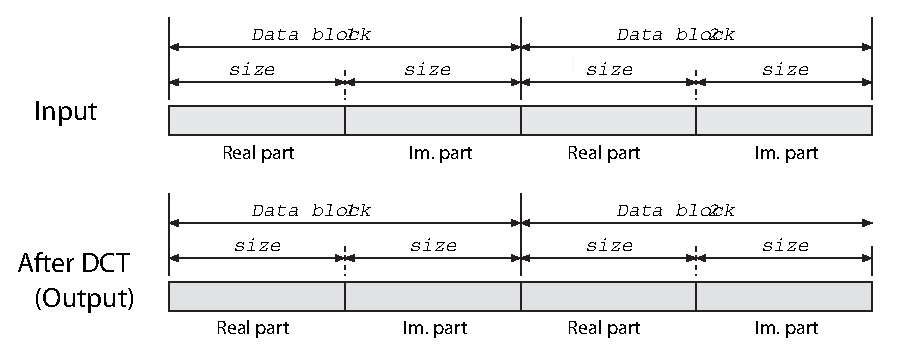
\includegraphics{fig/dct.eps}
\end{center}
The Discrete Cosine Transformation II is
\begin{displaymath}
 X_{k} =  \sqrt{\frac{2}{L}}c_{k}\sum_{l=0}^{L-1}
x_{l}\cos\left\{\frac{\pi}{L} k \left( l + \frac{1}{2} \right) \right\},
\;\;\; l = 0, 1, \cdots, L
\end{displaymath}
 where
 \begin{displaymath}
  c_{k}= \begin{cases}
         \;\;1 & ( 1 \le k \le L - 1 ) \\
         \;\; 1 / \sqrt{2} & (k = 0)
         \end{cases}
 \end{displaymath}
\par
\end{qsection}

\begin{options}
        \argm{l}{L}{DCT size}{256}
        \argm{I}{}{use complex number}{FALSE}
        \argm{d}{}{don't use FFT algorithm}{FALSE}
\end{options}

\begin{qsection}{EXAMPLE}
In this example, the DCT is evaluated from a complex-valued data file
{\em data.f} in float format
(real part: 256 points, imaginary part: 256 points),
and the output is written to {\em data.dct}:
\begin{quote}
  \verb!dct data.f -l 256 -I > data.dct!
\end{quote}
\end{qsection}

\begin{qsection}{SEE ALSO}
\hyperlink{fft}{fft},
\hyperlink{idct}{idct}
\end{qsection}

% ----------------------------------------------------------------- %
%             The Speech Signal Processing Toolkit (SPTK)           %
%             developed by SPTK Working Group                       %
%             http://sp-tk.sourceforge.net/                         %
% ----------------------------------------------------------------- %
%                                                                   %
%  Copyright (c) 1984-2007  Tokyo Institute of Technology           %
%                           Interdisciplinary Graduate School of    %
%                           Science and Engineering                 %
%                                                                   %
%                1996-2015  Nagoya Institute of Technology          %
%                           Department of Computer Science          %
%                                                                   %
% All rights reserved.                                              %
%                                                                   %
% Redistribution and use in source and binary forms, with or        %
% without modification, are permitted provided that the following   %
% conditions are met:                                               %
%                                                                   %
% - Redistributions of source code must retain the above copyright  %
%   notice, this list of conditions and the following disclaimer.   %
% - Redistributions in binary form must reproduce the above         %
%   copyright notice, this list of conditions and the following     %
%   disclaimer in the documentation and/or other materials provided %
%   with the distribution.                                          %
% - Neither the name of the SPTK working group nor the names of its %
%   contributors may be used to endorse or promote products derived %
%   from this software without specific prior written permission.   %
%                                                                   %
% THIS SOFTWARE IS PROVIDED BY THE COPYRIGHT HOLDERS AND            %
% CONTRIBUTORS "AS IS" AND ANY EXPRESS OR IMPLIED WARRANTIES,       %
% INCLUDING, BUT NOT LIMITED TO, THE IMPLIED WARRANTIES OF          %
% MERCHANTABILITY AND FITNESS FOR A PARTICULAR PURPOSE ARE          %
% DISCLAIMED. IN NO EVENT SHALL THE COPYRIGHT OWNER OR CONTRIBUTORS %
% BE LIABLE FOR ANY DIRECT, INDIRECT, INCIDENTAL, SPECIAL,          %
% EXEMPLARY, OR CONSEQUENTIAL DAMAGES (INCLUDING, BUT NOT LIMITED   %
% TO, PROCUREMENT OF SUBSTITUTE GOODS OR SERVICES; LOSS OF USE,     %
% DATA, OR PROFITS; OR BUSINESS INTERRUPTION) HOWEVER CAUSED AND ON %
% ANY THEORY OF LIABILITY, WHETHER IN CONTRACT, STRICT LIABILITY,   %
% OR TORT (INCLUDING NEGLIGENCE OR OTHERWISE) ARISING IN ANY WAY    %
% OUT OF THE USE OF THIS SOFTWARE, EVEN IF ADVISED OF THE           %
% POSSIBILITY OF SUCH DAMAGE.                                       %
% ----------------------------------------------------------------- %
\hypertarget{decimate}{}
\name{decimate}{decimation (data skipping)}{signal processing}

\begin{synopsis}
\item[decimate] [ --p $P$ ] [ --s $S$ ] [ --l $L$ ] [ {\em infile} ]
\end{synopsis}

\begin{qsection}{DESCRIPTION}
{\em decimate} picks up a sequence of input data
from {\em infile} (or standard input)
with interval $P$ and start number $S$,
sending the result to standard output.

If the input data is
\begin{displaymath}
 \bx(0), \bx(1), \bx(2), \dots
\end{displaymath}
then the output data is given by:
\begin{displaymath}
 \bx(S), \bx(S+P), \bx(S+2P), \bx(S+3P),\dots
\end{displaymath}
\par
Input and output data are in float format.
\end{qsection}

\begin{options}
	\argm{l}{L}{length of vector}{1}
	\argm{p}{P}{decimation period}{10}
	\argm{s}{S}{start sample}{0}
\end{options}

\begin{qsection}{EXAMPLE}
This example decimates input data from {\em data.f} file with interval 2,
interpolates 0 with interval 2, and then outputs the results to
the file {\em data.di}:
\begin{quote}
  \verb!decimate -p 2  < data.f | interpolate -p 2 > data.di!
\end{quote}
\end{qsection}

\begin{qsection}{SEE ALSO}
\hyperlink{interpolate}{interpolate}
\end{qsection}

\name{delay}{delay sequence}{signal processing}

\begin{synopsis}
\item [delay] [ --s $S$ ] [ --f ] [ {\em infile} ] 
\end{synopsis}

\begin{qsection}{DESCRIPTION}
 This command includes a delay on the signal in the input file.
 For example, if we want to delay the following data
\[ x(0), x(1), \ldots , x(T) \]
as
\[ \underbrace{0, \ldots , 0}_{S}, x(0), x(1), \ldots , x(T). \]
we only need to set the ``--s'' option to $S$
\[ \underbrace{0, \ldots , 0}_{S}, x(0), x(1), \ldots , x(T-S) \]
\par
The format of input and output is float.
\end{qsection}

\begin{options}
	\argm{s}{S}{start sample}{0}
	\argm{f}{}{keep file length}{False}
\end{options}

\begin{qsection}{EXAMPLE}
If we have the following data in the input {\em data.f} file
\begin{displaymath}
 1.0, 2.0, 3.0, 4.0, 5.0, 6.0
\end{displaymath}
and we use the command below
\begin{quote}
 \verb!delay -s 3 < data.f > data.delay!
\end{quote}
then the output file {\em data.delay} is 
\begin{displaymath}
 0.0, 0.0, 0.0, 1.0, 2.0, 3.0, 4.0, 5.0, 6.0
\end{displaymath}
As another example, if we want to keep the same size of the input file,
we can use the following command,
\begin{quote}
\verb!delay -s 3 -f < data.f > data.delay!
\end{quote}
and the output {\em data.delay} is
\begin{displaymath}
 0.0, 0.0, 0.0, 1.0, 2.0, 3.0
\end{displaymath}
\end{qsection}

%\begin{qsection}{SEE ALSO}
%none
%\end{qsection}

% ----------------------------------------------------------------- %
%             The Speech Signal Processing Toolkit (SPTK)           %
%             developed by SPTK Working Group                       %
%             http://sp-tk.sourceforge.net/                         %
% ----------------------------------------------------------------- %
%                                                                   %
%  Copyright (c) 1984-2007  Tokyo Institute of Technology           %
%                           Interdisciplinary Graduate School of    %
%                           Science and Engineering                 %
%                                                                   %
%                1996-2014  Nagoya Institute of Technology          %
%                           Department of Computer Science          %
%                                                                   %
% All rights reserved.                                              %
%                                                                   %
% Redistribution and use in source and binary forms, with or        %
% without modification, are permitted provided that the following   %
% conditions are met:                                               %
%                                                                   %
% - Redistributions of source code must retain the above copyright  %
%   notice, this list of conditions and the following disclaimer.   %
% - Redistributions in binary form must reproduce the above         %
%   copyright notice, this list of conditions and the following     %
%   disclaimer in the documentation and/or other materials provided %
%   with the distribution.                                          %
% - Neither the name of the SPTK working group nor the names of its %
%   contributors may be used to endorse or promote products derived %
%   from this software without specific prior written permission.   %
%                                                                   %
% THIS SOFTWARE IS PROVIDED BY THE COPYRIGHT HOLDERS AND            %
% CONTRIBUTORS "AS IS" AND ANY EXPRESS OR IMPLIED WARRANTIES,       %
% INCLUDING, BUT NOT LIMITED TO, THE IMPLIED WARRANTIES OF          %
% MERCHANTABILITY AND FITNESS FOR A PARTICULAR PURPOSE ARE          %
% DISCLAIMED. IN NO EVENT SHALL THE COPYRIGHT OWNER OR CONTRIBUTORS %
% BE LIABLE FOR ANY DIRECT, INDIRECT, INCIDENTAL, SPECIAL,          %
% EXEMPLARY, OR CONSEQUENTIAL DAMAGES (INCLUDING, BUT NOT LIMITED   %
% TO, PROCUREMENT OF SUBSTITUTE GOODS OR SERVICES; LOSS OF USE,     %
% DATA, OR PROFITS; OR BUSINESS INTERRUPTION) HOWEVER CAUSED AND ON %
% ANY THEORY OF LIABILITY, WHETHER IN CONTRACT, STRICT LIABILITY,   %
% OR TORT (INCLUDING NEGLIGENCE OR OTHERWISE) ARISING IN ANY WAY    %
% OUT OF THE USE OF THIS SOFTWARE, EVEN IF ADVISED OF THE           %
% POSSIBILITY OF SUCH DAMAGE.                                       %
% ----------------------------------------------------------------- %
\hypertarget{delta}{}
\name{delta}{delta calculation}{data processing}

\begin{synopsis}
	\item [delta] [ --m $M$ ] [ --l $L$ ] [ --t $T$ ] 
		[ --d ($fn$ $|$ $d_0$ [$d_1$ $\dots$]) ]
		[ --r $N_R$ $W_1$ [$W_2$] ]
 \item [\ ~~~~~~~]
 [ --R $N_R$ ${W_F}_{1}$ ${W_B}_{1}$ [${W_F}_{2}$ ${W_B}_{2}$]]
 [ --M $magic$ ] [ --n $N$ ] [ --e $e$ ][ {\em infile} ]
\end{synopsis}

\begin{qsection}{DESCRIPTION}
	{\em delta} calculates dynamic features from {\em infile} (or standard
	input), sending the result (static and dynamic features) to
        the standard output. Input and output are of the form:
    \begin{align}
	\mathrm{input}  & \dots, x_t(0), \dots, x_t(M), \dots \notag \\
	\mathrm{output} & \dots, x_t(0), \dots, x_t(M), \Delta^{(1)} x_t(0), \dots, \Delta^{(1)} x_t(M), \dots,
	\Delta^{(n)} x_t(0), \dots, \Delta^{(n)} x_t(M), \dots \notag
 \end{align}
Also, input and output data are in float format.
The dynamic feature vector $\Delta^{(n)}\bx_t$ can be
obtained from the static feature vector as follows.
 \begin{displaymath}
	\Delta^{(n)}\bx_t 
	= \sum_{\tau=-L^{(n)}}^{L^{(n)}} w^{(n)}(\tau)\bx_{t+\tau}
 \end{displaymath}
where $n$ is the order of the dynamic feature vector. For
example, when we evaluate the $\Delta^2$ parameter, $n=2$.
\end{qsection}

\begin{options}
	\argm{m}{M}{order of vector}{25}
	\argm{l}{L}{length of vector }{$M+1$}
	\argm{d}{(fn~|~d_0~[d_1~\dots])}{$fn$ is 
                the file name of the parameters $w^{(n)}(\tau)$
               	used when evaluating the dynamic feature vector.
                It is assumed that the number of coefficients
                to the left and to the right are the same. In case
                this is not true, then zeros are added to the
                shortest side.
                For example, if the coefficients are given by:
	 \begin{displaymath}
		w(-1), w(0), w(1), w(2), w(3)
	 \end{displaymath}
		then zeros must be added to the left as follows.
	 \begin{displaymath}
		0, 0, w(-1), w(0), w(1), w(2), w(3)
	 \end{displaymath}
		Instead of entering the filename $fn$,
                the coefficients(which compose the file $fn$)
                can be directly inputted from the command line.
                When the order of the dynamic feature vector is higher
                than one, then the sets of coefficients can be inputted
                one after the other as shown in the example below.
		This option cannot be used with the --r nor --R options.}{N/A}
	\argm{r}{N_R~W_1~[W_2]}{
		This option is used when $N_R$-th order dynamic parameters
                are used and the weighting coefficients $w^{(n)}(\tau)$
                are evaluated by regression.
                $N_R$ can be made equal to 1 or 2.
		The variables $W_1$ and $W_2$ represent the
                widths of the first and second order regression
                coefficients, respectively.
		The first order regression coefficients for
                $\Delta\bx_t$ at frame $t$ are evaluated as follows.
	 \begin{displaymath}
		\Delta\bx_t
		= \frac{\sum_{\tau=-W_1}^{W_1}\tau \bc_{t+\tau}}%
			{\sum_{\tau=-W_1}^{W_1}\tau^2}
	 \end{displaymath}
		For the second order regression coefficients,
		$a_2 = \sum_{\tau=-W_2}^{W_2} \tau^4$,
		$a_1 = \sum_{\tau=-W_2}^{W_2} \tau^2$,
		$a_0 = \sum_{\tau=-W_2}^{W_2} 1$
                and 
	 \begin{displaymath}
		\Delta^2\bx_t
		= \frac{2\sum_{\tau=-W_2}^{W_2}
				(a_0\tau^2 - a_1) \bx_{t+\tau}}
			{a_2a_0-a_1^2}
	 \end{displaymath}
 This option cannot be used with the --d nor --R options.}{N/A}
 \argm{R}{N_R~{W_F}_1~{W_B}_1[{W_F}_2~{W_B}_2]}{
Similarly to the --r option, by using this option, we can obtain
$N_{R}$-th order dynamic feature parameters  and the weighting
coefficients will be evaluated by regression. $N_{R}$ can be made equal
 to 1 or 2. The variables $W_{Fi}$ and $W_{Bi}$ represent the width of the
 $i$-th order regression
 coefficients in the forward and backward direction, respectively.
 Combining this option with the --M option, the regression coefficients can be evaluated skipping the magic
 number from the input.
 This option cannot be used with the --d nor --r options.
 }{N/A}
 \argm{M}{magic}{
 The magic number $magic$ can be skipped from the input during the calculation of
 the dynamic features. This option is valid
 only when the --R option is also specified.
 }{N/A}
 \argm{n}{N}{$N$ is the order of regression polynomial.
 Note that $N$ must be less than or equal to $\mathop{\rm max}\limits_{i=1,2}
 \left(W_{Fi} + W_{Bi}\right)$.}{N/A}
 \argm{e}{e}{
 small value added to diagonal component for calculating inverse matrix
 }{0.0}
\end{options}

\begin{qsection}{EXAMPLE}
In the example below, the first and second order dynamic features are calculated from 15-dimensional
coefficient vectors from {\em data.static} using windows whose width
are 1. The resultant
static and dynamic features are sent to {\em data.delta}:
 \begin{quote}
	\verb!delta -m 15 -r 2 1 1 data.static > data.delta!
 \end{quote}
	or
 \begin{quote}
	\verb!echo "-0.5 0 0.5" | x2x +af > delta! \\
	\verb!echo "1.0 -2.0 1.0" | x2x +af > accel! \\
	\verb!delta -m 15 -d delta -d accel data.static > data.delta!
 \end{quote}
Another example is presented bellow, where the first and second order
dynamic features are calculated from the scalar sequence in {\em
  data.f0}, sending windows with 2 units width and skipping the magic
number -1.0E15.
 \begin{quote}
	\verb!delta -l 1 -R 2 2 2 2 2 -M -1.0E15 data.f0 > data.delta!
 \end{quote}
\end{qsection}

\begin{qsection}{SEE ALSO}
\hyperlink{mlpg}{mlpg}
\end{qsection}

\name{df2}{two dimension digital filter}{digital filter}

\begin{synopsis}
 \item[df2] [ --f $f_0$ ] [ --p $f_1 \; b_1$ ] [ --z $f_2 \; b_2$ ] 
	    [ {\em infile} ]
 \end{synopsis}

 \begin{qsection}{DESCRIPTION}
 This command reads the input data file and passes it through a 2nd
  order digital filter. The central frequency and frequency band can
  be assigned through the options.
  The filter tranfer function is
 \[
   H(z)=\frac{1-2\exp(-\pi b_2/f_0)\cos(2\pi f_2/f_0)z^{-1} +
	\exp(-2\pi b_2/f_0)z^{-2}}
   {1-2\exp(-\pi b_1/f_0)\cos(2\pi f_1/f_0)z^{-1}+\exp(-2\pi b_1/f_0)z^{-2}}
 \]
 If this command is used in cascade, an arbitary filter can be
 designed using the options --p and --z.
 Input and output data are in float format.
 \end{qsection}

\begin{options}
	\argm{f}{f_0}{sampling frequency $f_0$[Hz]$B!%(B}{10000}
	\argm{p}{f_1 \; b_1}{center frequency $f_1$[Hz]
                and band width $b_1$[Hz] of pole}
		{N/A}
	\argm{z}{f_2 \; b_2}{center frequency $f_2$[Hz]
                and band width $b_2$[Hz] of zero}
		{N/A}
\end{options} 

\begin{qsection}{EXAMPLE}
The command below gives impulse response of a filter with
a pole at 2000Hz and a frequency band of 200Hz:
\begin{quote}
 \verb!impulse | df2 -p 2000 200 !
\end{quote}
\hspace{3cm}
\epsfxsize=4cm
\epsffile{fig/df2.eps} 
\end{qsection}

% ----------------------------------------------------------------- %
%             The Speech Signal Processing Toolkit (SPTK)           %
%             developed by SPTK Working Group                       %
%             http://sp-tk.sourceforge.net/                         %
% ----------------------------------------------------------------- %
%                                                                   %
%  Copyright (c) 1984-2007  Tokyo Institute of Technology           %
%                           Interdisciplinary Graduate School of    %
%                           Science and Engineering                 %
%                                                                   %
%                1996-2009  Nagoya Institute of Technology          %
%                           Department of Computer Science          %
%                                                                   %
% All rights reserved.                                              %
%                                                                   %
% Redistribution and use in source and binary forms, with or        %
% without modification, are permitted provided that the following   %
% conditions are met:                                               %
%                                                                   %
% - Redistributions of source code must retain the above copyright  %
%   notice, this list of conditions and the following disclaimer.   %
% - Redistributions in binary form must reproduce the above         %
%   copyright notice, this list of conditions and the following     %
%   disclaimer in the documentation and/or other materials provided %
%   with the distribution.                                          %
% - Neither the name of the SPTK working group nor the names of its %
%   contributors may be used to endorse or promote products derived %
%   from this software without specific prior written permission.   %
%                                                                   %
% THIS SOFTWARE IS PROVIDED BY THE COPYRIGHT HOLDERS AND            %
% CONTRIBUTORS "AS IS" AND ANY EXPRESS OR IMPLIED WARRANTIES,       %
% INCLUDING, BUT NOT LIMITED TO, THE IMPLIED WARRANTIES OF          %
% MERCHANTABILITY AND FITNESS FOR A PARTICULAR PURPOSE ARE          %
% DISCLAIMED. IN NO EVENT SHALL THE COPYRIGHT OWNER OR CONTRIBUTORS %
% BE LIABLE FOR ANY DIRECT, INDIRECT, INCIDENTAL, SPECIAL,          %
% EXEMPLARY, OR CONSEQUENTIAL DAMAGES (INCLUDING, BUT NOT LIMITED   %
% TO, PROCUREMENT OF SUBSTITUTE GOODS OR SERVICES; LOSS OF USE,     %
% DATA, OR PROFITS; OR BUSINESS INTERRUPTION) HOWEVER CAUSED AND ON %
% ANY THEORY OF LIABILITY, WHETHER IN CONTRACT, STRICT LIABILITY,   %
% OR TORT (INCLUDING NEGLIGENCE OR OTHERWISE) ARISING IN ANY WAY    %
% OUT OF THE USE OF THIS SOFTWARE, EVEN IF ADVISED OF THE           %
% POSSIBILITY OF SUCH DAMAGE.                                       %
% ----------------------------------------------------------------- %
\hypertarget{dfs}{}
\name{dfs}{digital filter in standard form}{digital filter}

\begin{synopsis}
\item[dfs] [ --a $K$ $a(1)$ $\dots$ $a(M)$ ] 
	   [ --b $b(0)$ $b(1)$ $\dots$ $b(N)$ ] 
	   [ --p {\em pfile} ] [ --z {\em zfile} ]
\item[\ ~~~] [ {\em infile} ]
\end{synopsis}

\begin{qsection}{DESCRIPTION}
{\em dfs} filters data from {\em infile} (or standard output) 
with a digital filter in standard form, 
sending the result to standard output.
  The filter transfer function is
\begin{displaymath}
  H(z) 
  = 
  K\frac{\displaystyle{\sum_{n=0}^{N}{b(n)z^{-n}}}}{1+\displaystyle{\sum_{m=1}^{M}{a(m)z^{-m}}}}
\end{displaymath}
\par
The format of input and output data is float.
\end{qsection}

\begin{options}
	\argm{a}{K \; a(1) \dots a(M)}{denominator coefficients,
                       where $K$ is the gain of the transfer function.}{N/A}
	\argm{b}{b(0) \; b(1) \dots b(N)}{numerator coefficients}
		{N/A}
	\argm{p}{pfile}{denominator coefficients file in float format
                as follows\\
		\hspace*{2ex}$K, a(1), \ldots, a(M)$\\[-1ex]}{NULL}
	\argm{z}{zfile}{numerator coefficients file in float format
                as follows\\
		\hspace*{2ex}$b(0), b(1), \ldots, b(N)$\\[-1ex]}{NULL}
	\desc{If {\bf --a}, {\bf --p} options are not assigned,
              the denominator and $K$ are made equal to 1.
              If {\bf --b}, {\bf --z} options are not assigned,
              the numerator is made equal to 1.}
\end{options}

\begin{qsection}{EXAMPLE}
If we want to see the impulse response of the following transfer
 function
\begin{displaymath}
  H(z)=\frac{1+2z^{-1}+z^{-2}}{1+0.9z^{-1}}
\end{displaymath}
the command below can be used
\begin{quote}
 \verb!impulse | dfs -a 1 0.9 -b 1 2 1 | dmp +f!
\end{quote}
\par
If we want to see the frequency response plot of the digital filter
whose coefficients are defined in float form by the files
{\em data.p, data.z}, then we can use the following:
\begin{quote}
 \verb!impulse | dfs -p data.p -z data.z | spec | fdrw | xgr!
\end{quote}
The files {\em data.p} and {\em data.z} can be constructed
using the command {\em x2x}.
\end{qsection}
 
% ----------------------------------------------------------------
%       Speech Signal Processing Toolkit (SPTK): version 3.0
%                      SPTK Working Group
% 
%                Department of Computer Science
%                Nagoya Institute of Technology
%                             and
%   Interdisciplinary Graduate School of Science and Engineering
%                Tokyo Institute of Technology
%                   Copyright (c) 1984-2000
%                     All Rights Reserved.
% 
% Permission is hereby granted, free of charge, to use and
% distribute this software and its documentation without
% restriction, including without limitation the rights to use,
% copy, modify, merge, publish, distribute, sublicense, and/or
% sell copies of this work, and to permit persons to whom this
% work is furnished to do so, subject to the following conditions:
% 
%   1. The code must retain the above copyright notice, this list
%      of conditions and the following disclaimer.
% 
%   2. Any modifications must be clearly marked as such.
%                                                                        
% NAGOYA INSTITUTE OF TECHNOLOGY, TOKYO INSITITUTE OF TECHNOLOGY,
% SPTK WORKING GROUP, AND THE CONTRIBUTORS TO THIS WORK DISCLAIM
% ALL WARRANTIES WITH REGARD TO THIS SOFTWARE, INCLUDING ALL
% IMPLIED WARRANTIES OF MERCHANTABILITY AND FITNESS, IN NO EVENT
% SHALL NAGOYA INSTITUTE OF TECHNOLOGY, TOKYO INSITITUTE OF
% TECHNOLOGY, SPTK WORKING GROUP, NOR THE CONTRIBUTORS BE LIABLE
% FOR ANY SPECIAL, INDIRECT OR CONSEQUENTIAL DAMAGES OR ANY
% DAMAGES WHATSOEVER RESULTING FROM LOSS OF USE, DATA OR PROFITS,
% WHETHER IN AN ACTION OF CONTRACT, NEGLIGENCE OR OTHER TORTIOUS
% ACTION, ARISING OUT OF OR IN CONNECTION WITH THE USE OR
% PERFORMANCE OF THIS SOFTWARE.
% ----------------------------------------------------------------
%
\name{dmp}{binary file dump}{data operation}

\begin{synopsis}
\item[dmp] [ --n $N$ ] [ --l $L$ ] [ +{\em type} ] [ $\%${\em form} ] [ {\em infile} ]
\end{synopsis}

\begin{qsection}{DESCRIPTION}
{\em dmp} converts data from {\em infile} (or standard input) 
to human readable form, 
one sample per line with line numbers, 
sending the result to standard output.
\end{qsection}

\begin{options}
	\argm{n}{N}{block order (0,...,n)}{EOD}
	\argm{l}{L}{block length  (1,...,l)}{EOD}
	\argp{t}{input data format\\
		\begin{tabular}{llcll} \\[-1ex]
			c & char (1byte) & \quad &
			s & short (2bytes) \\
			i & int (4bytes) & \quad &
			l & long (4bytes) \\
			f & float (4bytes) & \quad &
			d & double (8bytes)
		\end{tabular}\\\hspace*{\fill}}{f}
        \argh{form}{}{print format(printf style)}{N/A}

\end{options}

\begin{qsection}{EXAMPLE}
In this example, data is read from the input file
{\em data.f} in float format, and the enumerated data is sent
to the screen:
\begin{quote}
 \verb!dmp +f data.f!
\end{quote}
For example, if the {\em data.f} file has the following values
in float format
\begin{displaymath}
  1, 2, 3, 4, 5, 6, 7
\end{displaymath}
then the following output will be displayed on the screen:
\begin{quote}
  \verb!0       1! \\
  \verb!1       2! \\
  \verb!2       3! \\
  \verb!3       4! \\
  \verb!4       5! \\
  \verb!5       6! \\
  \verb!6       7!
\end{quote}
\par
In case we want to assign a block length:
\begin{quote}
 \verb!dmp -n 2 +f data.f!
\end{quote}
Then the output would be
\begin{quote}
  \verb!0       1! \\
  \verb!1       2! \\
  \verb!2       3! \\
  \verb!0       4! \\
  \verb!1       5! \\
  \verb!2       6! \\
  \verb!0       7!
\end{quote}
\par
If we want to print on the screen the unit impulse response of a digital
filter:
\begin{quote}
  \verb!impulse | dfs -a 1 0.9 | dmp!
\end{quote}
\par
If we want to print a sine wave then we can use the \%e option of
{\em printf} as follows:
\begin{quote}
  \verb!sin -p 30 | dmp %e!
\end{quote}
\par
If we want to represent the sine wave with three decimal points:
\begin{quote}
  \verb!sin -p 30 | dmp %.3e!
\end{quote}
\end{qsection}

\begin{qsection}{SEE ALSO}
x2x, fd
\end{qsection}

% ----------------------------------------------------------------- %
%             The Speech Signal Processing Toolkit (SPTK)           %
%             developed by SPTK Working Group                       %
%             http://sp-tk.sourceforge.net/                         %
% ----------------------------------------------------------------- %
%                                                                   %
%  Copyright (c) 1984-2007  Tokyo Institute of Technology           %
%                           Interdisciplinary Graduate School of    %
%                           Science and Engineering                 %
%                                                                   %
%                1996-2012  Nagoya Institute of Technology          %
%                           Department of Computer Science          %
%                                                                   %
% All rights reserved.                                              %
%                                                                   %
% Redistribution and use in source and binary forms, with or        %
% without modification, are permitted provided that the following   %
% conditions are met:                                               %
%                                                                   %
% - Redistributions of source code must retain the above copyright  %
%   notice, this list of conditions and the following disclaimer.   %
% - Redistributions in binary form must reproduce the above         %
%   copyright notice, this list of conditions and the following     %
%   disclaimer in the documentation and/or other materials provided %
%   with the distribution.                                          %
% - Neither the name of the SPTK working group nor the names of its %
%   contributors may be used to endorse or promote products derived %
%   from this software without specific prior written permission.   %
%                                                                   %
% THIS SOFTWARE IS PROVIDED BY THE COPYRIGHT HOLDERS AND            %
% CONTRIBUTORS "AS IS" AND ANY EXPRESS OR IMPLIED WARRANTIES,       %
% INCLUDING, BUT NOT LIMITED TO, THE IMPLIED WARRANTIES OF          %
% MERCHANTABILITY AND FITNESS FOR A PARTICULAR PURPOSE ARE          %
% DISCLAIMED. IN NO EVENT SHALL THE COPYRIGHT OWNER OR CONTRIBUTORS %
% BE LIABLE FOR ANY DIRECT, INDIRECT, INCIDENTAL, SPECIAL,          %
% EXEMPLARY, OR CONSEQUENTIAL DAMAGES (INCLUDING, BUT NOT LIMITED   %
% TO, PROCUREMENT OF SUBSTITUTE GOODS OR SERVICES; LOSS OF USE,     %
% DATA, OR PROFITS; OR BUSINESS INTERRUPTION) HOWEVER CAUSED AND ON %
% ANY THEORY OF LIABILITY, WHETHER IN CONTRACT, STRICT LIABILITY,   %
% OR TORT (INCLUDING NEGLIGENCE OR OTHERWISE) ARISING IN ANY WAY    %
% OUT OF THE USE OF THIS SOFTWARE, EVEN IF ADVISED OF THE           %
% POSSIBILITY OF SUCH DAMAGE.                                       %
% ----------------------------------------------------------------- %
\hypertarget{dtw}{}
\name{dtw}{dynamic time warping}{dynamic time warping}
\begin{synopsis}
\item[dtw] [ --m $M$ ]  [ --l $L$ ]  [ --t $T$ ]  [ --r $R$ ]
           [ --n $N$ ]  [ --p $P$ ]
 \item [\ ~~~~~~~] [ --s $Scorefile$ ]  [ --v $Vitfile$ ]
 {\em reffile} [ {\em infile} ]
\end{synopsis}

\begin{qsection}{DESCRIPTION}
 {\em dtw} carries out dynamic time warping between
 the test data vectors from {\em infile} (or standard input)
 and the reference data vectors from {\em reffile},
 and sends the result to standard output.
 The result is the concatenated sequence
 of the test and the reference data vectors
 along with the Viterbi path.
 If --s option is specified,
 the score calculated by dynamic time warping,
 that is, the distance between the test data and the reference data
 is output and sent to {\em Scorefile}.
 If --v option is specified,
 the concatenated frame number sequence
 along the Viterbi path
 is output and sent to {\em Vitfile}.

 For example, suppose that the test and the reference data vectors are
 \begin{align}
  \mathrm{test} :\;\; & \bx(0), \bx(1), \dots, \bx(T_x - 1), \bx(T_x), \notag \\
  \mathrm{reference}  :\;\; & \by(0), \by(1), \dots, \by(T_y - 1), \by(T_y), \notag
 \end{align}
 where $T_x$ and $T_y$ are the length of the test and reference data vectors,
 respectively,p
 and the following Viterbi sequences
 \begin{align}
  \mathrm{test} :\;\; & \bx(\phi_x(0)), \bx(\phi_x(1)), \dots, \bx(\phi_x(T_x - 1)),
  \bx(\phi_{x}(T_x)), \notag \\
  \mathrm{reference}  :\;\; & \by(\phi_y(0)), \by(\phi_y(1)), \dots,
  \by(\phi_y(T_y - 1)), \by(\phi_y(T_y)), \notag
 \end{align}
 are obtained, where $\phi_x(\cdot)$ and $\phi_x(\cdot)$ are the function which
 maps the frame number of test/reference data
 into the corresponding Viterbi frame number, respectively.
 In addition, the relation $\phi_x(T_x)=\phi_y(T_y)$ holds.
 Then, the following sequence
 \begin{align}
  \bx(\phi_x(0)), \by(\phi_y(0)),
  \bx(\phi_x(1)), \by(\phi_y(1)),
  \dots, \bx(\phi_{x}(T_x)), \by(\phi_y(T_y)) \notag
 \end{align}
 are sent to the standard output.
 If --v option is specified, the following sequence
 \begin{align}
  \phi_x(0), \phi_y(0),
  \phi_x(1), \phi_y(1),
  \dots, \phi_{x}(T_x), \phi_y(T_y) \notag
 \end{align}
 are sent to the {\em Vitfile}.

 Both input and output files are in float format. However,
 the {\em Vitfile} which contains the Viterbi frame number
 sequence is in int format.
\end{qsection}
\begin{options}
 \argm{m}{M}{order of vector}{0}
 \argm{l}{L}{dimention of vector}{M+1}
 \argm{t}{T}{number of test vectors}{N/A}
 \argm{r}{R}{number of reference vectors}{N/A}
 \argm{n}{N}{type of norm used for calculation of local cost\\
 \begin{tabular}{ll} \\[-1ex]
  $N=1$ & ~~~$L_{1}$-norm\\
  $N=2$ & ~~~$L_{2}$-norm\\
 \end{tabular}\\\hspace*{\fill}}{2}
 \argm{p}{P}{local path constraint\\
 candidates of constraint are shown in figure \ref{fig:dtw_cand}.}{5}
 \argm{s}{Scorefile}{output score of the dynamic time warping
 to ${Scorefile}$. }{FALSE}
 \argm{v}{Vitfile}{output frame number sequence along the Viterbi
 path to ${Vitfile}$.}{FALSE}
\end{options}

\begin{qsection}{EXAMPLE}
 In the example below, a dynamic time warping between the scalar
 sequence from {\em data.test} and
 the sequence from {\em data.ref} is carried out and
 the concatenated sequence are written to {\em data.out}.
\begin{quote}
 \verb!dtw -l 1 data.ref < data.test > data.out!
\end{quote}
\end{qsection}

\begin{figure}[htbp]
 \begin{center}
  \begin{tabular}{cccc} \\[-1ex]
   &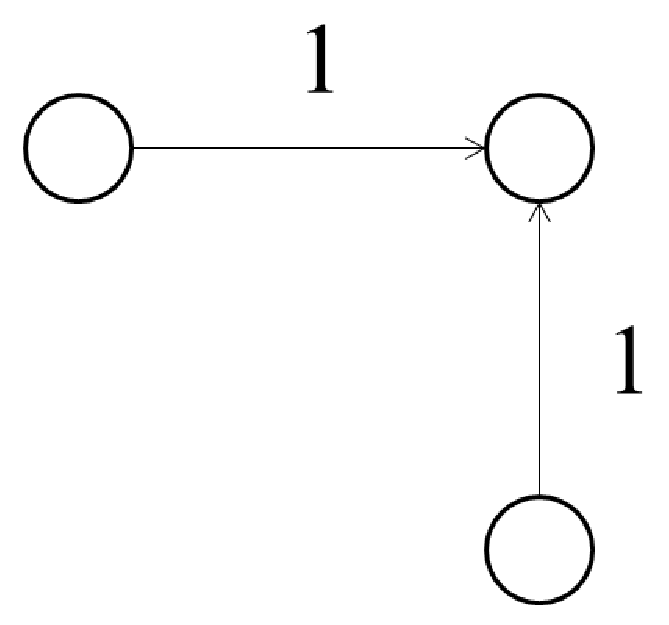
\includegraphics[height=2cm]{fig/path1.eps}
   &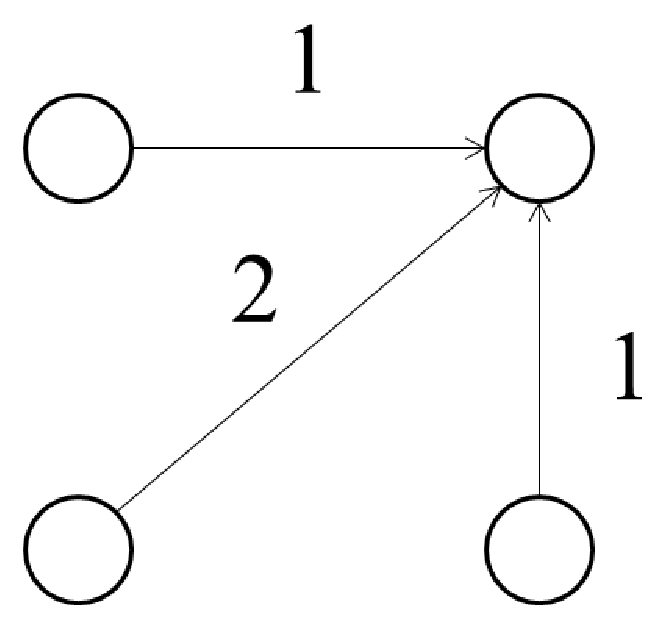
\includegraphics[height=2cm]{fig/path2.eps}
   &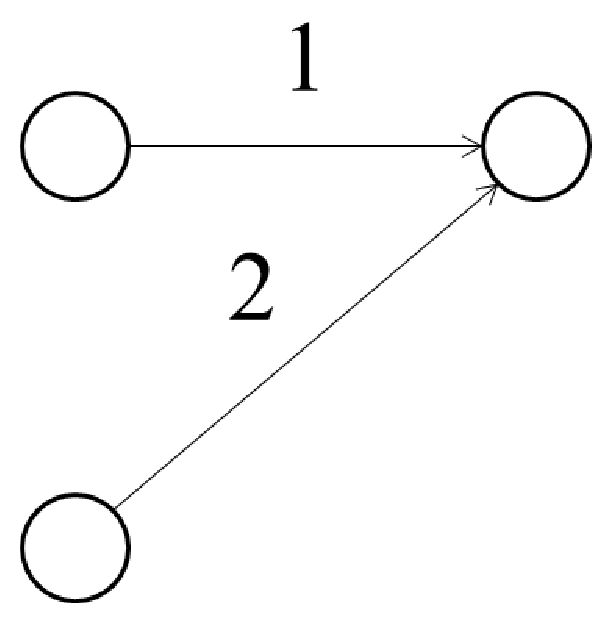
\includegraphics[height=2cm]{fig/path3.eps}\\
   &$P=1$&$P=2$&$P=3$\\
   &&&\\
   &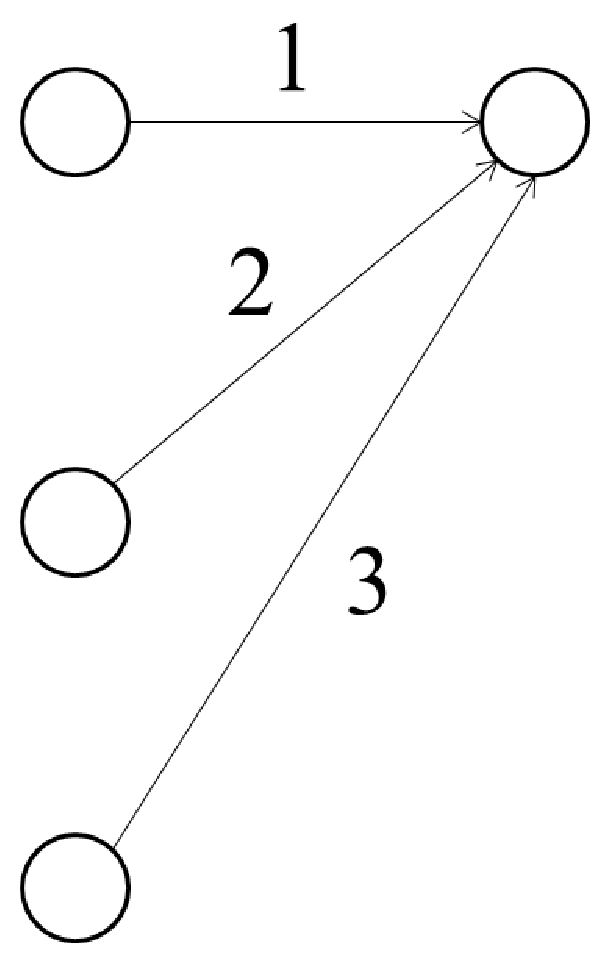
\includegraphics[height=3cm]{fig/path4.eps}
       &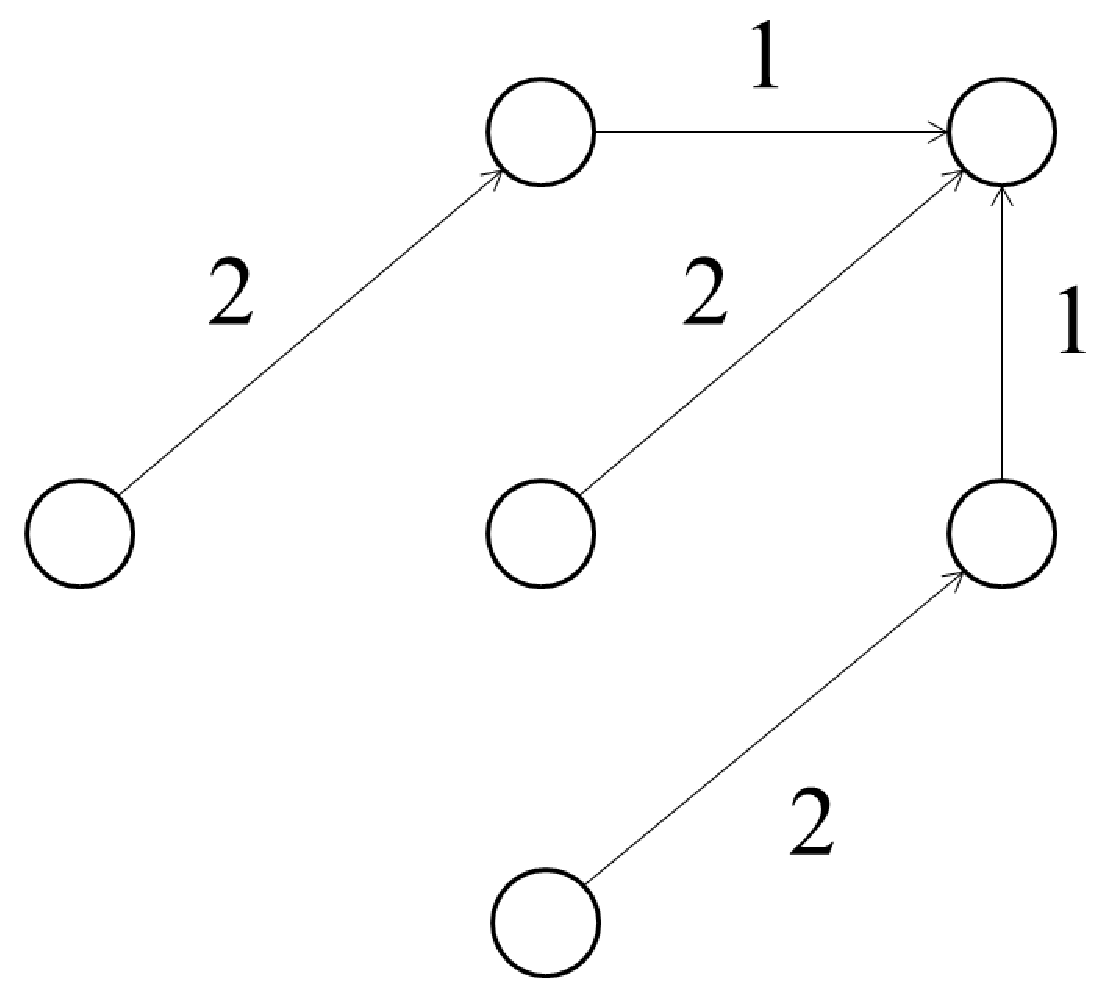
\includegraphics[height=3cm]{fig/path5.eps}
   &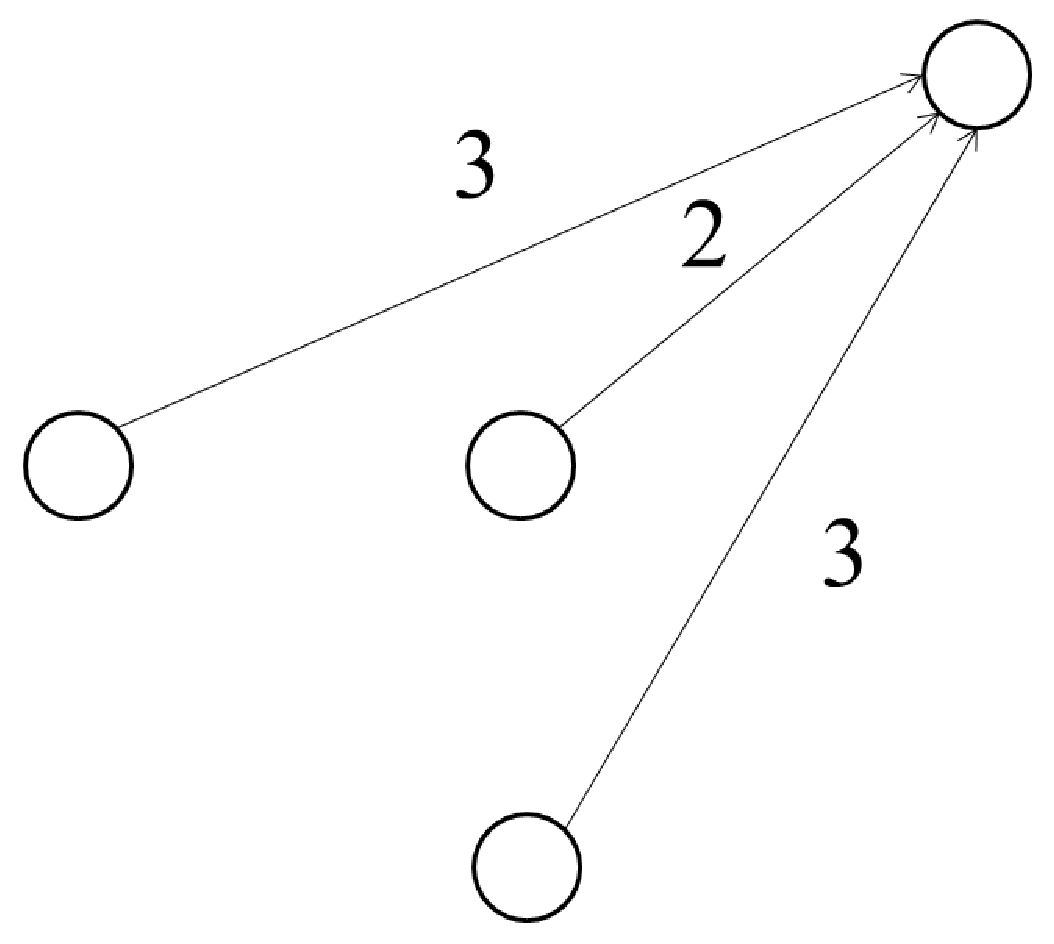
\includegraphics[height=3cm]{fig/path6.eps}\\
   &$P=4$&$P=5$&$P=6$\\
   &&&\\
   &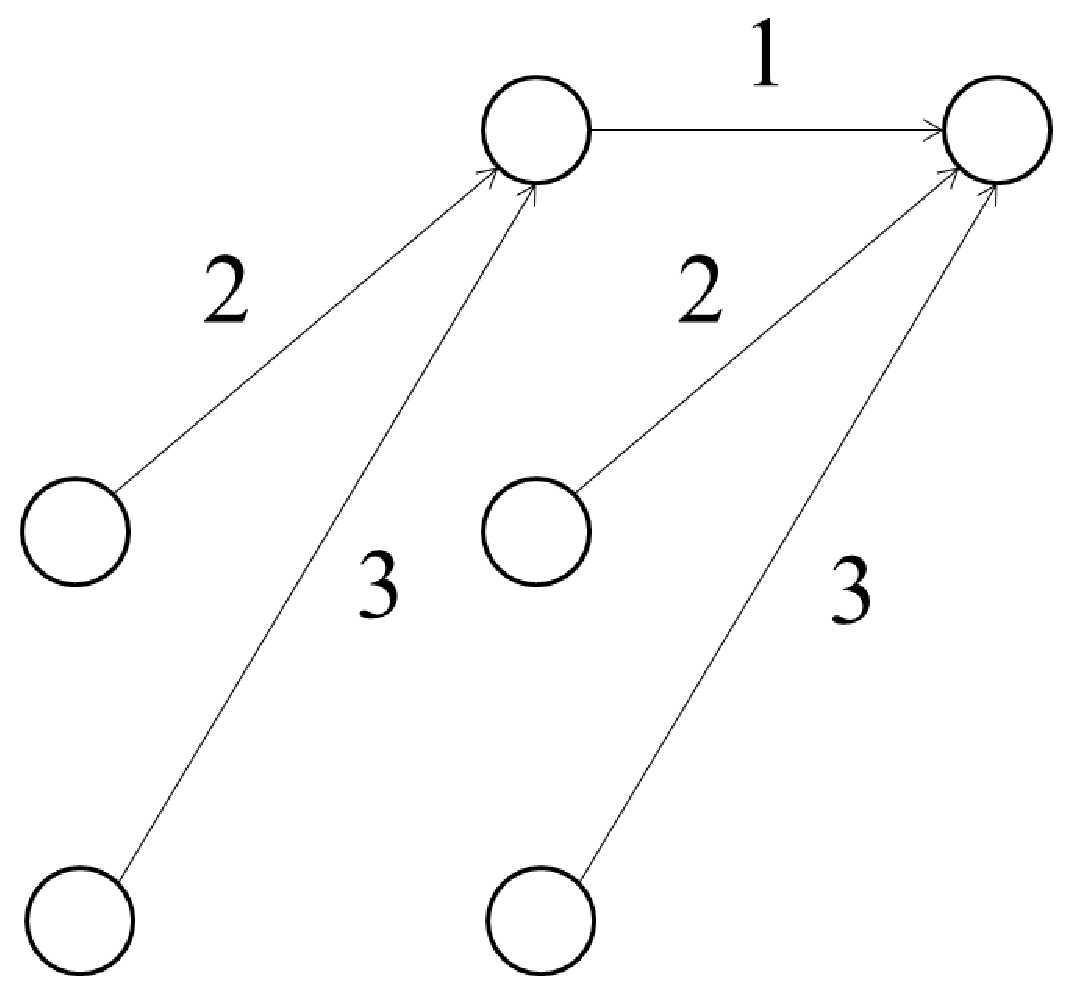
\includegraphics[height=3cm]{fig/path7.eps}
       &&\\
   &$P=7$&&\\
  \end{tabular}
 \end{center}
 \caption{candidates of local path constraint}
 \label{fig:dtw_cand}
\end{figure}

% \begin{qsection}{SEE ALSO}
% \hyperlink{vc}{vc}
% \end{qsection}


\name{ds}{$B%5%s%W%j%s%0%l!<%HJQ49!J%@%&%s%5%s%W%j%s%0!K(B}%
{$B%5%s%W%j%s%0%l!<%HJQ49(B}

\begin{synopsis}
\item[ds] [ --e $E$ ] [ --s $S$ ] [ {\em infile} ]
\end{synopsis}

\begin{qsection}{DESCRIPTION}
$B%@%&%s%5%s%W%j%s%0$r9T$J$$$^$9!%(B
\par
$B%G!<%?7A<0$OF~NO!$=PNO$H$b(Bfloat$B7A<0$G$9!%(B
$B%U%#%k%?78?t$O<!$N$b$N$,MQ$$$i$l$^$9!%(B

\begin{tabular}{ll} \\[-1zh]
	$S=21$ & lpfcoef.2to1 \\
	$S=43$ & lpfcoef.4to3 \\
	$S=52,s=54$ & lpfcoef.5to2up \\
	& lpfcoef.5to2dn \\
\end{tabular}

$B$J$*!$%U%!%$%k%?78?t$N%U%!%$%k$O(BASCII$B7A<0$H$J$C$F$$$^$9!%(B
\end{qsection}

\begin{options}
	\argm{s}{S}{$BJQ49%?%$%W!%(B \\
		\begin{tabular}{ll} \\[-1zh]
			$S=21$ & $BHfN((B $2 : 1$ $B$G%@%&%s%5%s%W%j%s%0(B \\
			$S=43$ & $BHfN((B $4 : 3$ $B$G%@%&%s%5%s%W%j%s%0(B \\
			$S=52$ & $BHfN((B $5 : 2$ $B$G%@%&%s%5%s%W%j%s%0(B \\
			$S=54$ & $BHfN((B $5 : 4$ $B$G%@%&%s%5%s%W%j%s%0(B
		\end{tabular}\\\hspace*{\fill}}{21}
\end{options}

\begin{qsection}{EXAMPLE}
float$B7A<0$NI8K\2=<~GH?t(B16kHz$B$N2;@<%G!<%?(B {\em data.16} $B$rI8K\2=<~GH?t(B8kHz$B$K(B
$B%@%&%s%5%s%W%j%s%0$7!$(B {\em data.8} $B$K=PNO$9$k(B:
\begin{quote}
\verb! ds data.16 > data.8 !
\end{quote}
\end{qsection}

%\begin{qsection}{SEE ALSO}
%
%\end{qsection}

% ----------------------------------------------------------------- %
%             The Speech Signal Processing Toolkit (SPTK)           %
%             developed by SPTK Working Group                       %
%             http://sp-tk.sourceforge.net/                         %
% ----------------------------------------------------------------- %
%                                                                   %
%  Copyright (c) 1984-2007  Tokyo Institute of Technology           %
%                           Interdisciplinary Graduate School of    %
%                           Science and Engineering                 %
%                                                                   %
%                1996-2010  Nagoya Institute of Technology          %
%                           Department of Computer Science          %
%                                                                   %
% All rights reserved.                                              %
%                                                                   %
% Redistribution and use in source and binary forms, with or        %
% without modification, are permitted provided that the following   %
% conditions are met:                                               %
%                                                                   %
% - Redistributions of source code must retain the above copyright  %
%   notice, this list of conditions and the following disclaimer.   %
% - Redistributions in binary form must reproduce the above         %
%   copyright notice, this list of conditions and the following     %
%   disclaimer in the documentation and/or other materials provided %
%   with the distribution.                                          %
% - Neither the name of the SPTK working group nor the names of its %
%   contributors may be used to endorse or promote products derived %
%   from this software without specific prior written permission.   %
%                                                                   %
% THIS SOFTWARE IS PROVIDED BY THE COPYRIGHT HOLDERS AND            %
% CONTRIBUTORS "AS IS" AND ANY EXPRESS OR IMPLIED WARRANTIES,       %
% INCLUDING, BUT NOT LIMITED TO, THE IMPLIED WARRANTIES OF          %
% MERCHANTABILITY AND FITNESS FOR A PARTICULAR PURPOSE ARE          %
% DISCLAIMED. IN NO EVENT SHALL THE COPYRIGHT OWNER OR CONTRIBUTORS %
% BE LIABLE FOR ANY DIRECT, INDIRECT, INCIDENTAL, SPECIAL,          %
% EXEMPLARY, OR CONSEQUENTIAL DAMAGES (INCLUDING, BUT NOT LIMITED   %
% TO, PROCUREMENT OF SUBSTITUTE GOODS OR SERVICES; LOSS OF USE,     %
% DATA, OR PROFITS; OR BUSINESS INTERRUPTION) HOWEVER CAUSED AND ON %
% ANY THEORY OF LIABILITY, WHETHER IN CONTRACT, STRICT LIABILITY,   %
% OR TORT (INCLUDING NEGLIGENCE OR OTHERWISE) ARISING IN ANY WAY    %
% OUT OF THE USE OF THIS SOFTWARE, EVEN IF ADVISED OF THE           %
% POSSIBILITY OF SUCH DAMAGE.                                       %
% ----------------------------------------------------------------- %
\hypertarget{echo2}{}
\name{echo2}{echo arguments to the standard error}{others}

\begin{synopsis}
\item[echo2] [ --n ] [ argument ]
\end{synopsis}

\begin{qsection}{DESCRIPTION}

{\em echo2} sends its command line arguments to standard error.

\end{qsection}

\begin{options}
	\argm{n}{}{no output newline}{FALSE}
\end{options}

\begin{qsection}{EXAMPLE}
This example prints ''error!'' in the standard error output:
\begin{quote}
  \begin{verbatim}
  echo2 -n "error!"
  \end{verbatim}
\end{quote}
\end{qsection}

% ----------------------------------------------------------------- %
%             The Speech Signal Processing Toolkit (SPTK)           %
%             developed by SPTK Working Group                       %
%             http://sp-tk.sourceforge.net/                         %
% ----------------------------------------------------------------- %
%                                                                   %
%  Copyright (c) 1984-2007  Tokyo Institute of Technology           %
%                           Interdisciplinary Graduate School of    %
%                           Science and Engineering                 %
%                                                                   %
%                1996-2010  Nagoya Institute of Technology          %
%                           Department of Computer Science          %
%                                                                   %
% All rights reserved.                                              %
%                                                                   %
% Redistribution and use in source and binary forms, with or        %
% without modification, are permitted provided that the following   %
% conditions are met:                                               %
%                                                                   %
% - Redistributions of source code must retain the above copyright  %
%   notice, this list of conditions and the following disclaimer.   %
% - Redistributions in binary form must reproduce the above         %
%   copyright notice, this list of conditions and the following     %
%   disclaimer in the documentation and/or other materials provided %
%   with the distribution.                                          %
% - Neither the name of the SPTK working group nor the names of its %
%   contributors may be used to endorse or promote products derived %
%   from this software without specific prior written permission.   %
%                                                                   %
% THIS SOFTWARE IS PROVIDED BY THE COPYRIGHT HOLDERS AND            %
% CONTRIBUTORS "AS IS" AND ANY EXPRESS OR IMPLIED WARRANTIES,       %
% INCLUDING, BUT NOT LIMITED TO, THE IMPLIED WARRANTIES OF          %
% MERCHANTABILITY AND FITNESS FOR A PARTICULAR PURPOSE ARE          %
% DISCLAIMED. IN NO EVENT SHALL THE COPYRIGHT OWNER OR CONTRIBUTORS %
% BE LIABLE FOR ANY DIRECT, INDIRECT, INCIDENTAL, SPECIAL,          %
% EXEMPLARY, OR CONSEQUENTIAL DAMAGES (INCLUDING, BUT NOT LIMITED   %
% TO, PROCUREMENT OF SUBSTITUTE GOODS OR SERVICES; LOSS OF USE,     %
% DATA, OR PROFITS; OR BUSINESS INTERRUPTION) HOWEVER CAUSED AND ON %
% ANY THEORY OF LIABILITY, WHETHER IN CONTRACT, STRICT LIABILITY,   %
% OR TORT (INCLUDING NEGLIGENCE OR OTHERWISE) ARISING IN ANY WAY    %
% OUT OF THE USE OF THIS SOFTWARE, EVEN IF ADVISED OF THE           %
% POSSIBILITY OF SUCH DAMAGE.                                       %
% ----------------------------------------------------------------- %
\hypertarget{excite}{}
\name{excite}{generate excitation}{signal generation,speech analysis and synthesis}

\begin{synopsis}
\item [excite] [ --p $P$ ] [ --i $I$ ] [ --n ] [ --s $S$ ] [ {\em infile} ]
\end{synopsis}

\begin{qsection}{DESCRIPTION}
{\em excite} generates an excitation sequence 
from pitch period information from {\em infile} (or standard input), 
sending the result to standard output. 
When the pitch period is nonzero (i.e. voiced), 
the excitation sequence consists of a pulse train at that pitch. 
When the pitch period is zero (i.e. unvoiced),
the excitation sequence consists of Gaussian or M-sequence noise.

Input and output data are in float format.
\end{qsection}

\begin{options}
	\argm{p}{P}{frame period}{100}
	\argm{i}{I}{interpolation period}{1}
	\argm{n}{}{gauss/M-sequence for unvoiced\\
                   default is M-sequence}{FALSE}
	\argm{s}{S}{seed for nrand for Gaussian noise}{1}
\end{options}

\begin{qsection}{EXAMPLE}
In the example below, the excitation is generated from the
{\em data.p} file and passed through a LPC synthesis filter
whose coefficients are in the {\em data.lpc} file.
The speech signal is output to the {\em data.syn} file.
\begin{quote}
 \verb!excite < data.p | poledf data.lpc > data.syn!
\end{quote} 
In case we use Gaussian noise to generate are an unvoiced sound:
\begin{quote}
 \verb!excite -n < data.p | poledf data.lpc > data.syn!
\end{quote}
\end{qsection}

\begin{qsection}{SEE ALSO}
\hyperlink{poledf}{poledf}
\end{qsection}

% ----------------------------------------------------------------
%       Speech Signal Processing Toolkit (SPTK): version 3.0
%                      SPTK Working Group
% 
%                Department of Computer Science
%                Nagoya Institute of Technology
%                             and
%   Interdisciplinary Graduate School of Science and Engineering
%                Tokyo Institute of Technology
%                   Copyright (c) 1984-2000
%                     All Rights Reserved.
% 
% Permission is hereby granted, free of charge, to use and
% distribute this software and its documentation without
% restriction, including without limitation the rights to use,
% copy, modify, merge, publish, distribute, sublicense, and/or
% sell copies of this work, and to permit persons to whom this
% work is furnished to do so, subject to the following conditions:
% 
%   1. The code must retain the above copyright notice, this list
%      of conditions and the following disclaimer.
% 
%   2. Any modifications must be clearly marked as such.
%                                                                        
% NAGOYA INSTITUTE OF TECHNOLOGY, TOKYO INSITITUTE OF TECHNOLOGY,
% SPTK WORKING GROUP, AND THE CONTRIBUTORS TO THIS WORK DISCLAIM
% ALL WARRANTIES WITH REGARD TO THIS SOFTWARE, INCLUDING ALL
% IMPLIED WARRANTIES OF MERCHANTABILITY AND FITNESS, IN NO EVENT
% SHALL NAGOYA INSTITUTE OF TECHNOLOGY, TOKYO INSITITUTE OF
% TECHNOLOGY, SPTK WORKING GROUP, NOR THE CONTRIBUTORS BE LIABLE
% FOR ANY SPECIAL, INDIRECT OR CONSEQUENTIAL DAMAGES OR ANY
% DAMAGES WHATSOEVER RESULTING FROM LOSS OF USE, DATA OR PROFITS,
% WHETHER IN AN ACTION OF CONTRACT, NEGLIGENCE OR OTHER TORTIOUS
% ACTION, ARISING OUT OF OR IN CONNECTION WITH THE USE OR
% PERFORMANCE OF THIS SOFTWARE.
% ----------------------------------------------------------------
%
\hypertarget{extract}{}
\name{extract}{extract vector}%
{vector quantization}

\begin{synopsis}
\item [extract] [ --l $L$ ] [ --i $I$ ]  {\em indexfile}  [ {\em infile} ] 
\end{synopsis}

\begin{qsection}{DESCRIPTION}
{\em extract} extracts selected vectors 
from {\em infile} (or standard input), 
sending the result to standard output. 
{\em indexfile} contains a previously-computed sequence of 
codebook indices corresponding to the input vectors.  
Only those input vectors whose codebook index (from {\em indexfile}) 
matches the index given by the ``--i'' option 
are sent through to standard output.
\end{qsection}

\begin{options}
	\argm{l}{L}{order of vector}{10}
	\argm{i}{I}{codebook index}{0}
\end{options}

\begin{qsection}{EXAMPLE}
In the example below, a 10 order vector file {\em data.v}
in float format is quantized using a previously obtained
codebook {\em data.idx} and writes to the output file {\em data.ex}
the vectors which were quantized to the index 0 codeword.
\begin{quote}
\verb!extract -i 0 data.idx data.v > data.ex!
\end{quote}
\end{qsection}

\begin{qsection}{SEE ALSO}
\hyperlink{ivq}{ivq},
\hyperlink{vq}{vq}
\end{qsection}

% ----------------------------------------------------------------
%       Speech Signal Processing Toolkit (SPTK): version 3.0
%                      SPTK Working Group
% 
%                Department of Computer Science
%                Nagoya Institute of Technology
%                             and
%   Interdisciplinary Graduate School of Science and Engineering
%                Tokyo Institute of Technology
%                   Copyright (c) 1984-2000
%                     All Rights Reserved.
% 
% Permission is hereby granted, free of charge, to use and
% distribute this software and its documentation without
% restriction, including without limitation the rights to use,
% copy, modify, merge, publish, distribute, sublicense, and/or
% sell copies of this work, and to permit persons to whom this
% work is furnished to do so, subject to the following conditions:
% 
%   1. The code must retain the above copyright notice, this list
%      of conditions and the following disclaimer.
% 
%   2. Any modifications must be clearly marked as such.
%                                                                        
% NAGOYA INSTITUTE OF TECHNOLOGY, TOKYO INSITITUTE OF TECHNOLOGY,
% SPTK WORKING GROUP, AND THE CONTRIBUTORS TO THIS WORK DISCLAIM
% ALL WARRANTIES WITH REGARD TO THIS SOFTWARE, INCLUDING ALL
% IMPLIED WARRANTIES OF MERCHANTABILITY AND FITNESS, IN NO EVENT
% SHALL NAGOYA INSTITUTE OF TECHNOLOGY, TOKYO INSITITUTE OF
% TECHNOLOGY, SPTK WORKING GROUP, NOR THE CONTRIBUTORS BE LIABLE
% FOR ANY SPECIAL, INDIRECT OR CONSEQUENTIAL DAMAGES OR ANY
% DAMAGES WHATSOEVER RESULTING FROM LOSS OF USE, DATA OR PROFITS,
% WHETHER IN AN ACTION OF CONTRACT, NEGLIGENCE OR OTHER TORTIOUS
% ACTION, ARISING OUT OF OR IN CONNECTION WITH THE USE OR
% PERFORMANCE OF THIS SOFTWARE.
% ----------------------------------------------------------------
%
\hypertarget{fd}{}
\name{fd}{file dump}{data operation}

\begin{synopsis}
 \item [fd] [ --a $A$ ] [ --n $N$ ] [ --m $M$ ] [ --{\em ent} ] 
	    [ +{\em type} ] [ $\%${\em form} ] [ {\em infile} ]
\end{synopsis}

\begin{qsection}{DESCRIPTION}
{\em fd} converts data from {\em infile} (or standard input) 
to human-readable multi-column format, 
sending the result to standard output.
\end{qsection}

\begin{options}
	\argm{a}{A}{address}{0}
	\argm{n}{N}{initial value for numbering}{0}
	\argm{m}{M}{modulo for numbering}{EOF}
	\argm{{\em ent}}{}{number of data in each line}{0}
	\argp{t}{data type\\
		\begin{tabular}{llcll} \\[-1ex]
			c & char (1byte) & \quad &
			s & short (2bytes) \\
			i & int (4bytes) & \quad &
			l & long (4bytes) \\
			f & float (4bytes) & \quad &
			d & double (8bytes) 
		\end{tabular}\\\hspace*{\fill}}{c}
        \argh{form}{}{print format(printf style)}{N/A}
\end{options}

\begin{qsection}{EXAMPLE}
 This example displays the speech data in ``sample.wav'' with
 the corresponding addresses:
\begin{quote}
 \verb!fd -a 0 sample.wav!
\end{quote}
 Results:\\
\verb!000000  52 49 46 46 9a 15 00 00 57 41 56 45 66 6d 74 20 |RIFF....WAVEfmt |!\\
\verb!000010  10 00 00 00 01 00 01 00 40 1f 00 00 40 1f 00 00 |........@...@...|!\\
\verb!000020  01 00 08 00 64 61 74 61 76 15 00 00 8a 8a 8f 99 |....datav.......|!

\begin{center}
 $\vdots$\\
\end{center}
\end{qsection}

\begin{qsection}{SEE ALSO}
\hyperlink{dmp}{dmp}
\end{qsection}

\name{fdrw}{draw a graph}{plotting graphs}

\begin{synopsis}
\item[fdrw] [ --F $F$ ] [ --R $R$ ] [ --W $W$ ] [ --H $H$ ] [ --o $xo \; yo$ ] 
            [ --g $G$ ] [ --m $M$ ]   
\item[\ ~~~~~] [ --l $L$ ] [ --p $P$ ] [ --n $N$ ] [ --t $T$ ] 
	       [ --y $ymin \; ymax$ ] [ --z $Z$ ] [ --b ]  
\item[\ ~~~~~] [ {\em infile} ]
\end{synopsis}

\begin{qsection}{DESCRIPTION}
This command connects through a straight line the input data in float
format.
\par
The output includes the sequence of commands so that it can be plotted
(FP5301 protocol)
\end{qsection}

\begin{options}
	\argm{F}{F}{factor}{1}
	\argm{R}{R}{rotation angle}{0}
	\argm{W}{W}{width of figure($\times 100$mm)}{1}
	\argm{H}{H}{height of figure($\times 100$mm)}{1}
	\argm{o}{xo \; yo}{origin in mm}{20 25}
	\argm{g}{G}{draw grid($0 \sim 2$)
                    Please refer to ``fig'' command.}{1}
	\argm{m}{M}{line type($1 \sim 5$)\\
	\hspace*{2mm}1:~solid~~2:~dotted~~3:~dot and dash~~4:~broken~~5:~dash}{0}
	\argm{l}{L}{line pitch}{0}
	\argm{p}{P}{pen number($1 \sim 10$)��}{1}
	\argm{n}{N}{number of sample}{0}
	\argm{t}{T}{rotation of coordinate axis. when $T=-1$, the
                    reference point is on the top-left. when $T=1$
                    the reference point is on the botton-right.}{0}
	\argm{y}{ymin \; ymax}{scaling factor for $y$ axis}{-1 1}
	\argm{z}{Z}{This option is used when data is written
                    recursively in the $y$ axis. the distance between
                    two graphs in the $y$ axis are given by $Z$.}{0}
	\argm{b}{}{bar graph mode}{FALSE}
	\desc[1zh]{The $x$ axis scaling is automaticaly done so that
                every point in the input file is plotted in equal interval
                for the assigned width.
                When {\bf --n} option is omitted and number of
                input sample is below 5000, then the block size is made
                equal to number of samples.
                When the number of samples is above 5000,
                then the block size is made equal to 5000.}
	\desc{When the {\bf --y} option is omitted,
		the input data minimum value is made equal to $ymin$
                and the maximum value is made equal to $ymax$.}
\end{options}

\begin{qsection}{EXAMPLE}
In the example below, the impulse response of digital filter is
drawed on the X window environment:
\begin{quote}
  \verb!impulse | dfs -a 1 0.8 0.5 | fdrw -h 0.3 | xgr!
\end{quote}
Tha graph width is 10cm and its height is 3cm.
\par
The next example draws on the X window environment the magnitude of
frequency response of digital filter:
\begin{quote}
  \verb!impulse | dfs -a 1 0.8 0.5 | spec | fdrw -y -60 40 | xgr!
\end{quote}
The $y$ axis goes from $-60$dB to $40$dB.
\par
The running spectrum can be draw on the X window environment by:
\begin{quote}
 \verb!fig -g 0 -w 0.4 << EOF ! \\
 \verb!����x 0 5 !\\
 \verb!����xscale 0 1 2 3 4 5 !\\
 \verb!����xname "FREQUENCY (kHz)"!\\
 \verb!EOF!\\
 \verb!spec < data |\ !\\
 \verb!fdrw -w 0.4 -h 0.2 -g 0 -n 129 -y -30 30 -z 3 |\ !\\
 \verb!xgr !
\end{quote}
The command {\em psgr} prints the output in laser printer in the
same way that it is printed on the screen.
Since the {\em fdrw} command includes a sequence of commands
for plotter machine(FP5301 protocol) in the output file,
its output can be directly sent to a printer.
\end{qsection}

\begin{qsection}{SEE ALSO}
 fig, xgr, psgr
\end{qsection}

\name{fft}{$BJ#AG?tNs$N9bB.%U!<%j%(JQ49(B}{none}

\begin{synopsis}
\item[fft] [ --l $L$ ] [ --m $M$] [ --\{ A $|$ R $|$ I $|$ P \} ] 
	   [ {\em infile} ] 
\end{synopsis}

\begin{qsection}{DESCRIPTION}
$BJ#AG?tNs$r(B{\em infile} $B$+$iFI$_9~$_!$(BFFT $B%"%k%4%j%:%`$K$h$j(BDFT $B$r<B9T$7$^$9!%(B
{\em infile} $B$N;XDj$,$J$$$H$-$K$O!$I8=`F~NO$+$i%G!<%?$,FI$_9~$^$l$^$9!%(B
$B%G!<%?7A<0$OF~=PNO$H$b(Bfloat $B7A$G!$F~=PNO%G!<%?$N=g=x$O<!$NDL$j$G$9!%(B
\[
 \begin{array}{lll}
\mbox{$BF~NO7ONs(B} & \overbrace{\framebox[4.5cm]{$B<B!!It(B}}^{M+1} &
	   \overbrace{\framebox[4.5cm]{$B5u!!It(B}}^{M+1} \\
		& \makebox[4.5cm]{0\hfill $M$} &
		\makebox[4.5cm]{0\hfill $M$}
\end{array}
\]
\[
\begin{array}{lll}
\mbox{$B=PNO7ONs(B} & \overbrace{\framebox[4.5cm]{$B<B!!It(B}}^{L} &
	   \overbrace{\framebox[4.5cm]{$B5u!!It(B}}^{L} \\
		& \makebox[4.5cm]{0\hfill $L-1$} &
		\makebox[4.5cm]{0\hfill $L-1$}
\end{array}
\]
\end{qsection}

\begin{options}
	\argm{l}{L}{$B%U!<%j%(JQ49$N%5%$%:!%(B2 $B$N$Y$->h$G;XDj!%(B}{256}
	\argm{m}{M}{$BJ#AG?tNs$N<!?t!%(B}{L-1}
	\argm{A}{}{$B?6I}%9%Z%/%H%k$r=PNO!%(B}{FALSE}
	\argm{R}{}{$B<BIt$N$_$r=PNO!%(B}{FALSE}
	\argm{I}{}{$B5uIt$N$_$r=PNO!%(B}{FALSE}
	\argm{P}{}{$B%Q%o!<%9%Z%/%H%k$r=PNO!%(B}{FALSE}
\end{options}

\begin{qsection}{EXAMPLE}
float$B7A<0$N%U%!%$%k(B {\em data.f} $B$K$"$kJ#AG?tNs!J<BIt(B256$BE@!$5uIt(B256$BE@!K$N(B DFT $B$N?6I}$r5a$a!$(B{\em data.dft} $B$K=PNO$9$k(B:
\begin{quote}
  \verb!fft data.f -l 256 -A > data.dft!
\end{quote}
\end{qsection}

%\begin{qsection}{BUGS}
% FFT $B$N%5%$%:$O(B1024 $B0J2<!%(B
%\end{qsection}

\begin{qsection}{SEE ALSO}
  fftr, spec, phase
\end{qsection}

% ----------------------------------------------------------------- %
%             The Speech Signal Processing Toolkit (SPTK)           %
%             developed by SPTK Working Group                       %
%             http://sp-tk.sourceforge.net/                         %
% ----------------------------------------------------------------- %
%                                                                   %
%  Copyright (c) 1984-2007  Tokyo Institute of Technology           %
%                           Interdisciplinary Graduate School of    %
%                           Science and Engineering                 %
%                                                                   %
%                1996-2011  Nagoya Institute of Technology          %
%                           Department of Computer Science          %
%                                                                   %
% All rights reserved.                                              %
%                                                                   %
% Redistribution and use in source and binary forms, with or        %
% without modification, are permitted provided that the following   %
% conditions are met:                                               %
%                                                                   %
% - Redistributions of source code must retain the above copyright  %
%   notice, this list of conditions and the following disclaimer.   %
% - Redistributions in binary form must reproduce the above         %
%   copyright notice, this list of conditions and the following     %
%   disclaimer in the documentation and/or other materials provided %
%   with the distribution.                                          %
% - Neither the name of the SPTK working group nor the names of its %
%   contributors may be used to endorse or promote products derived %
%   from this software without specific prior written permission.   %
%                                                                   %
% THIS SOFTWARE IS PROVIDED BY THE COPYRIGHT HOLDERS AND            %
% CONTRIBUTORS "AS IS" AND ANY EXPRESS OR IMPLIED WARRANTIES,       %
% INCLUDING, BUT NOT LIMITED TO, THE IMPLIED WARRANTIES OF          %
% MERCHANTABILITY AND FITNESS FOR A PARTICULAR PURPOSE ARE          %
% DISCLAIMED. IN NO EVENT SHALL THE COPYRIGHT OWNER OR CONTRIBUTORS %
% BE LIABLE FOR ANY DIRECT, INDIRECT, INCIDENTAL, SPECIAL,          %
% EXEMPLARY, OR CONSEQUENTIAL DAMAGES (INCLUDING, BUT NOT LIMITED   %
% TO, PROCUREMENT OF SUBSTITUTE GOODS OR SERVICES; LOSS OF USE,     %
% DATA, OR PROFITS; OR BUSINESS INTERRUPTION) HOWEVER CAUSED AND ON %
% ANY THEORY OF LIABILITY, WHETHER IN CONTRACT, STRICT LIABILITY,   %
% OR TORT (INCLUDING NEGLIGENCE OR OTHERWISE) ARISING IN ANY WAY    %
% OUT OF THE USE OF THIS SOFTWARE, EVEN IF ADVISED OF THE           %
% POSSIBILITY OF SUCH DAMAGE.                                       %
% ----------------------------------------------------------------- %
\hypertarget{fft2}{}
\name{fft2}{2-dimensional FFT for complex sequence}{signal processing}

\begin{synopsis}
\item[fft2] [ --l $L$ ] [ --m $M_1 \; M_2$ ] [ --t ] [ --c ] [ --q ] 
            [ --\{ A $|$ R $|$ I $|$ P \} ]  
\item[\ ~~~~] [ {\em infile} ]  
\end{synopsis}

\begin{qsection}{DESCRIPTION}
{\em fft2} uses the 2-dimensional Fast Fourier Transform (FFT) algorithm 
to calculate the 2-dimensional Discrete Fourier Transform (DFT) 
of complex-valued input data from {\em infile} (or standard input), 
sending the result to standard output. 
The input and output data is in float format, arranged as follows.
\begin{center}
\leavevmode
\includegraphics{fig/fft2.eps}
\end{center}
\end{qsection}

\begin{options}
	\argm{l}{L}{FFT size  power of 2}{64}
	\argm{m}{M_1 \; M_2}{order of sequence ($M_1\times M_2$).
			If file size $k$ is smaller than $64^2\times 2$
			and $\sqrt{k\div 2}$ is integer value, $M_1=M_2=\sqrt{k\div 2}$. 
			Otherwise output error message to standard error output 
			and then terminate.}{$64 , M_1$}
	\argm{t}{}{Output results in transposed form.
		\begin{center}
		\leavevmode
		\includegraphics{fig/fft2-trans.eps}
		\end{center}~}{FALSE}
	\argm{c}{}{When results are transposed, 1 boundary data is copied from the
	opposite side, and then output $(L+1)\times (L+1)$ data.
		\begin{center}	
		\leavevmode
		\includegraphics{fig/fft2-comp.eps}
		\end{center}~}{FALSE}
	\argm{q}{}{Output first $1/4$ data of FFT results only.
		   As in the above c option, boundary data is compensated and 
		   $(\frac{L}{2}+1)\times(\frac{L}{2}+1)$ data are output.
		\begin{center}
		\leavevmode
		\includegraphics{fig/fft2-quad.eps}
		\end{center}~}{FALSE} %\hspace*{\fill}
	\argm{A}{}{amplitude}{FALSE}
	\argm{R}{}{real part}{FALSE}
	\argm{I}{}{imaginary part}{FALSE}
	\argm{P}{}{output power spectrum}{FALSE}
\end{options}

\begin{qsection}{EXAMPLE}
This example reads a sequence of 2-dimensional complex numbers in float format
from {\em data.f} file, evaluates its 2-dimensional DFT and outputs it to {\em
data.dft} file:
\begin{quote}
  \verb!fft2 -A data.f > data.dft!
\end{quote}
\end{qsection}

\begin{qsection}{SEE ALSO}
\hyperlink{fft}{fft},
\hyperlink{fftr2}{fftr2},
\hyperlink{ifft}{ifft}
\end{qsection}

% ----------------------------------------------------------------- %
%             The Speech Signal Processing Toolkit (SPTK)           %
%             developed by SPTK Working Group                       %
%             http://sp-tk.sourceforge.net/                         %
% ----------------------------------------------------------------- %
%                                                                   %
%  Copyright (c) 1984-2007  Tokyo Institute of Technology           %
%                           Interdisciplinary Graduate School of    %
%                           Science and Engineering                 %
%                                                                   %
%                1996-2011  Nagoya Institute of Technology          %
%                           Department of Computer Science          %
%                                                                   %
% All rights reserved.                                              %
%                                                                   %
% Redistribution and use in source and binary forms, with or        %
% without modification, are permitted provided that the following   %
% conditions are met:                                               %
%                                                                   %
% - Redistributions of source code must retain the above copyright  %
%   notice, this list of conditions and the following disclaimer.   %
% - Redistributions in binary form must reproduce the above         %
%   copyright notice, this list of conditions and the following     %
%   disclaimer in the documentation and/or other materials provided %
%   with the distribution.                                          %
% - Neither the name of the SPTK working group nor the names of its %
%   contributors may be used to endorse or promote products derived %
%   from this software without specific prior written permission.   %
%                                                                   %
% THIS SOFTWARE IS PROVIDED BY THE COPYRIGHT HOLDERS AND            %
% CONTRIBUTORS "AS IS" AND ANY EXPRESS OR IMPLIED WARRANTIES,       %
% INCLUDING, BUT NOT LIMITED TO, THE IMPLIED WARRANTIES OF          %
% MERCHANTABILITY AND FITNESS FOR A PARTICULAR PURPOSE ARE          %
% DISCLAIMED. IN NO EVENT SHALL THE COPYRIGHT OWNER OR CONTRIBUTORS %
% BE LIABLE FOR ANY DIRECT, INDIRECT, INCIDENTAL, SPECIAL,          %
% EXEMPLARY, OR CONSEQUENTIAL DAMAGES (INCLUDING, BUT NOT LIMITED   %
% TO, PROCUREMENT OF SUBSTITUTE GOODS OR SERVICES; LOSS OF USE,     %
% DATA, OR PROFITS; OR BUSINESS INTERRUPTION) HOWEVER CAUSED AND ON %
% ANY THEORY OF LIABILITY, WHETHER IN CONTRACT, STRICT LIABILITY,   %
% OR TORT (INCLUDING NEGLIGENCE OR OTHERWISE) ARISING IN ANY WAY    %
% OUT OF THE USE OF THIS SOFTWARE, EVEN IF ADVISED OF THE           %
% POSSIBILITY OF SUCH DAMAGE.                                       %
% ----------------------------------------------------------------- %
\hypertarget{fftcep}{}
\name{fftcep}{FFT cepstral analysis}{signal processing}

\begin{synopsis}
\item[fftcep] [ --m $M$ ] [ --l $L$ ] [ --j $J$ ] [ --k $K$ ] 
	    [ --e $E$ ] [ {\em infile} ] 
\end{synopsis}

\begin{qsection}{DESCRIPTION}
{\em fftcep} uses FFT cepstral analysis to calculate the cepstrum 
from windowed framed input data in {\em infile} (or standard input), 
sending the result to standard output.
The windowed input time domain sequence of length $L$ is of the form:
\begin{displaymath}
  x(0),x(1),\dots,x(L-1)
\end{displaymath}
\par
Input and output data are in float format.
\par
Also, the improved cepstral analysis method \cite{ref:icep-IECE} may be used if the
number of iterations $J$ and the acceleration factor $K$ are given.
\end{qsection}

\begin{options}
	\argm{m}{M}{order of cepstrum}{25}
	\argm{l}{L}{frame length}{256}
	\argm{j}{J}{number of iteration}{0}
	\argm{k}{K}{acceleration factor}{0.0}
	\argm{e}{E}{epsilon}{0.0}
\end{options}

\begin{qsection}{EXAMPLE}
In the example below, speech data in float format is read from
{\em data.f} and the cepstral coefficients are output to {\em data.cep}:
\begin{quote}
  \verb!frame +f < data.f | window | fftcep > data.cep !
\end{quote}
\end{qsection}

\begin{qsection}{SEE ALSO}
\hyperlink{uels}{uels}
\end{qsection}

% ----------------------------------------------------------------- %
%             The Speech Signal Processing Toolkit (SPTK)           %
%             developed by SPTK Working Group                       %
%             http://sp-tk.sourceforge.net/                         %
% ----------------------------------------------------------------- %
%                                                                   %
%  Copyright (c) 1984-2007  Tokyo Institute of Technology           %
%                           Interdisciplinary Graduate School of    %
%                           Science and Engineering                 %
%                                                                   %
%                1996-2016  Nagoya Institute of Technology          %
%                           Department of Computer Science          %
%                                                                   %
% All rights reserved.                                              %
%                                                                   %
% Redistribution and use in source and binary forms, with or        %
% without modification, are permitted provided that the following   %
% conditions are met:                                               %
%                                                                   %
% - Redistributions of source code must retain the above copyright  %
%   notice, this list of conditions and the following disclaimer.   %
% - Redistributions in binary form must reproduce the above         %
%   copyright notice, this list of conditions and the following     %
%   disclaimer in the documentation and/or other materials provided %
%   with the distribution.                                          %
% - Neither the name of the SPTK working group nor the names of its %
%   contributors may be used to endorse or promote products derived %
%   from this software without specific prior written permission.   %
%                                                                   %
% THIS SOFTWARE IS PROVIDED BY THE COPYRIGHT HOLDERS AND            %
% CONTRIBUTORS "AS IS" AND ANY EXPRESS OR IMPLIED WARRANTIES,       %
% INCLUDING, BUT NOT LIMITED TO, THE IMPLIED WARRANTIES OF          %
% MERCHANTABILITY AND FITNESS FOR A PARTICULAR PURPOSE ARE          %
% DISCLAIMED. IN NO EVENT SHALL THE COPYRIGHT OWNER OR CONTRIBUTORS %
% BE LIABLE FOR ANY DIRECT, INDIRECT, INCIDENTAL, SPECIAL,          %
% EXEMPLARY, OR CONSEQUENTIAL DAMAGES (INCLUDING, BUT NOT LIMITED   %
% TO, PROCUREMENT OF SUBSTITUTE GOODS OR SERVICES; LOSS OF USE,     %
% DATA, OR PROFITS; OR BUSINESS INTERRUPTION) HOWEVER CAUSED AND ON %
% ANY THEORY OF LIABILITY, WHETHER IN CONTRACT, STRICT LIABILITY,   %
% OR TORT (INCLUDING NEGLIGENCE OR OTHERWISE) ARISING IN ANY WAY    %
% OUT OF THE USE OF THIS SOFTWARE, EVEN IF ADVISED OF THE           %
% POSSIBILITY OF SUCH DAMAGE.                                       %
% ----------------------------------------------------------------- %
\hypertarget{fftr}{}
\name{fftr}{FFT for real sequence}{signal processing}

\begin{synopsis}
 \item[fftr] [ --l $L$ ] [ --m $M$] [ --\{ A $|$ R $|$ I $|$ P \} ] [ --H ]
             [ {\em infile} ] 
\end{synopsis}

\begin{qsection}{DESCRIPTION}
{\em fftr} uses the Fast Fourier Transform (FFT) algorithm 
to calculate the Discrete Fourier Transform (DFT) 
of real-valued input data in {\em infile} (or standard input), 
and sends the result to standard output. 
To specify the FFT size, --l option can be used.
Also, --m option can be used to pad the input data with zeros.
When $M + 1 \leq L$,  the input data is padded
with $L - M - 1$ zeros. When $M + 1 > L$, {\em fftr} terminates
with error messages.
The input and output data is in float format, 
arranged as below.
\begin{displaymath}
\begin{array}{lll}
\mbox{Input sequence} & 
\overbrace{\framebox[4.5cm]{$x_0, x_1, \ldots, x_{M}, 0,
                                        \ldots,0$}}^{L}  & \\
                & \makebox[4.5cm]{0\hfill $L-1$} &
\end{array}
\end{displaymath}
\begin{displaymath}
\begin{array}{lll}
\mbox{Output sequence} & \overbrace{\framebox[4.5cm]{real part}}^{L} &
           \overbrace{\framebox[4.5cm]{imaginary part}}^{L} \\
                & \makebox[4.5cm]{0\hfill $L-1$} &
                \makebox[4.5cm]{0\hfill $L-1$}
\end{array}
\end{displaymath}
\end{qsection}

\begin{options}
        \argm{l}{L}{FFT size power of 2}{256}
        \argm{m}{M}{order of sequence}{L-1}
        \argm{A}{}{output magnitude}{FALSE}
        \argm{R}{}{output only real part}{FALSE}
        \argm{I}{}{output only imaginary part}{FALSE}
        \argm{P}{}{output power spectrum}{FALSE}
        \argm{H}{}{output half size}{FALSE}
\end{options}

\begin{qsection}{EXAMPLE}
In the example below, a sine wave is passed through a Blackman window,
its DFT is evaluated and the magnitude is plotted:
\begin{quote}
  \verb!sin -p 30 | window | fftr -A | fdrw | xgr!
\end{quote}

\end{qsection}

\begin{qsection}{SEE ALSO}
\hyperlink{fft}{fft},
\hyperlink{fft2}{fft2},
\hyperlink{fftr2}{fftr2},
\hyperlink{ifft}{ifft}
\hyperlink{ifftr}{ifftr}
\hyperlink{ifft2}{ifft2}
\hyperlink{spec}{spec},
\hyperlink{phase}{phase}
\end{qsection}

% ----------------------------------------------------------------- %
%             The Speech Signal Processing Toolkit (SPTK)           %
%             developed by SPTK Working Group                       %
%             http://sp-tk.sourceforge.net/                         %
% ----------------------------------------------------------------- %
%                                                                   %
%  Copyright (c) 1984-2007  Tokyo Institute of Technology           %
%                           Interdisciplinary Graduate School of    %
%                           Science and Engineering                 %
%                                                                   %
%                1996-2016  Nagoya Institute of Technology          %
%                           Department of Computer Science          %
%                                                                   %
% All rights reserved.                                              %
%                                                                   %
% Redistribution and use in source and binary forms, with or        %
% without modification, are permitted provided that the following   %
% conditions are met:                                               %
%                                                                   %
% - Redistributions of source code must retain the above copyright  %
%   notice, this list of conditions and the following disclaimer.   %
% - Redistributions in binary form must reproduce the above         %
%   copyright notice, this list of conditions and the following     %
%   disclaimer in the documentation and/or other materials provided %
%   with the distribution.                                          %
% - Neither the name of the SPTK working group nor the names of its %
%   contributors may be used to endorse or promote products derived %
%   from this software without specific prior written permission.   %
%                                                                   %
% THIS SOFTWARE IS PROVIDED BY THE COPYRIGHT HOLDERS AND            %
% CONTRIBUTORS "AS IS" AND ANY EXPRESS OR IMPLIED WARRANTIES,       %
% INCLUDING, BUT NOT LIMITED TO, THE IMPLIED WARRANTIES OF          %
% MERCHANTABILITY AND FITNESS FOR A PARTICULAR PURPOSE ARE          %
% DISCLAIMED. IN NO EVENT SHALL THE COPYRIGHT OWNER OR CONTRIBUTORS %
% BE LIABLE FOR ANY DIRECT, INDIRECT, INCIDENTAL, SPECIAL,          %
% EXEMPLARY, OR CONSEQUENTIAL DAMAGES (INCLUDING, BUT NOT LIMITED   %
% TO, PROCUREMENT OF SUBSTITUTE GOODS OR SERVICES; LOSS OF USE,     %
% DATA, OR PROFITS; OR BUSINESS INTERRUPTION) HOWEVER CAUSED AND ON %
% ANY THEORY OF LIABILITY, WHETHER IN CONTRACT, STRICT LIABILITY,   %
% OR TORT (INCLUDING NEGLIGENCE OR OTHERWISE) ARISING IN ANY WAY    %
% OUT OF THE USE OF THIS SOFTWARE, EVEN IF ADVISED OF THE           %
% POSSIBILITY OF SUCH DAMAGE.                                       %
% ----------------------------------------------------------------- %
\hypertarget{fftr2}{}
\name{fftr2}{2-dimensional FFT for real sequence}{signal processing}

\begin{synopsis}
\item[fftr2] [ --l $L$ ] [ --m $M_1 \; M_2$ ] [ --t ] [ --c ] [ --q ] 
	     [ --\{ A $|$ R $|$ I $|$ P \} ] [ {\em infile} ] 
\end{synopsis}

\begin{qsection}{DESCRIPTION}
{\em fftr2} uses the 2-dimensional Fast Fourier Transform (FFT) algorithm 
to calculate the 2-dimensional Discrete Fourier Transform (DFT) 
of real-valued input data in {\em infile} (or standard input), 
and sends the result to standard output. 
The input and output data is in float format, arranged as follows.
\begin{center}
 \leavevmode
 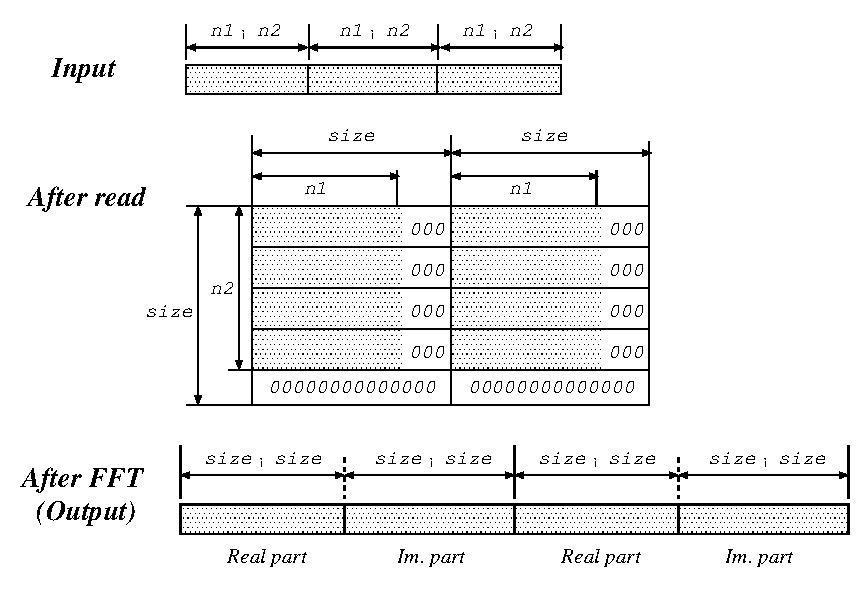
\includegraphics{fig/fftr2.eps}
\end{center}
\end{qsection}

\begin{options}
	\argm{l}{L}{FFT size  power of 2}{64}
	\argm{m}{M_1 \; M_2}{order of sequence ($M_1\times M_2$).
			If the file size $k$ is smaller than $64^2$
			and $\sqrt{k}$ is an integer value, then $M_1=M_2=\sqrt{k}$.
			Otherwise, output error message is sent to standard error output
			and then the command terminates.}{$64 , M_1$}
	\argm{t}{}{Output results in transposed form (see also \hyperlink{fft2}{fft2}).}{FALSE}
	\argm{c}{}{When results are transposed, 1 boundary data is copied from the
	opposite side, and then data whose size is $(L+1)\times (L+1)$ is output. (see also \hyperlink{fft2}{fft2}).}{FALSE}
	\argm{q}{}{Output first $1/4$ data of FFT results only.
		   As in --c option, boundary data is compensated and 
		   data whose size is $(\frac{L}{2}+1)\times(\frac{L}{2}+1)$ is output
		   (see also \hyperlink{fft2}{fft2}).}{FALSE}
	\argm{A}{}{output amplitude}{FALSE}
	\argm{R}{}{output only real part}{FALSE}
	\argm{I}{}{output only imaginary part}{FALSE}
	\argm{P}{}{output power spectrum}{FALSE}
\end{options}

\begin{qsection}{EXAMPLE}
This example reads a sequence of 2-dimensional real numbers in float format
from {\em data.f} file, evaluates its 2-dimensional DFT and outputs results to {\em 
data.dft} file:
\begin{quote}
  \verb!fftr2 -A data.f > data.dft!
\end{quote}
\end{qsection}

\begin{qsection}{SEE ALSO}
\hyperlink{fft}{fft},
\hyperlink{fft2}{fft2},
\hyperlink{fftr}{fftr},
\hyperlink{ifftr}{ifft}
\hyperlink{ifft2}{ifft2}
\hyperlink{ifftr}{ifftr}
\end{qsection}
 
% ----------------------------------------------------------------- %
%             The Speech Signal Processing Toolkit (SPTK)           %
%             developed by SPTK Working Group                       %
%             http://sp-tk.sourceforge.net/                         %
% ----------------------------------------------------------------- %
%                                                                   %
%  Copyright (c) 1984-2007  Tokyo Institute of Technology           %
%                           Interdisciplinary Graduate School of    %
%                           Science and Engineering                 %
%                                                                   %
%                1996-2009  Nagoya Institute of Technology          %
%                           Department of Computer Science          %
%                                                                   %
% All rights reserved.                                              %
%                                                                   %
% Redistribution and use in source and binary forms, with or        %
% without modification, are permitted provided that the following   %
% conditions are met:                                               %
%                                                                   %
% - Redistributions of source code must retain the above copyright  %
%   notice, this list of conditions and the following disclaimer.   %
% - Redistributions in binary form must reproduce the above         %
%   copyright notice, this list of conditions and the following     %
%   disclaimer in the documentation and/or other materials provided %
%   with the distribution.                                          %
% - Neither the name of the SPTK working group nor the names of its %
%   contributors may be used to endorse or promote products derived %
%   from this software without specific prior written permission.   %
%                                                                   %
% THIS SOFTWARE IS PROVIDED BY THE COPYRIGHT HOLDERS AND            %
% CONTRIBUTORS "AS IS" AND ANY EXPRESS OR IMPLIED WARRANTIES,       %
% INCLUDING, BUT NOT LIMITED TO, THE IMPLIED WARRANTIES OF          %
% MERCHANTABILITY AND FITNESS FOR A PARTICULAR PURPOSE ARE          %
% DISCLAIMED. IN NO EVENT SHALL THE COPYRIGHT OWNER OR CONTRIBUTORS %
% BE LIABLE FOR ANY DIRECT, INDIRECT, INCIDENTAL, SPECIAL,          %
% EXEMPLARY, OR CONSEQUENTIAL DAMAGES (INCLUDING, BUT NOT LIMITED   %
% TO, PROCUREMENT OF SUBSTITUTE GOODS OR SERVICES; LOSS OF USE,     %
% DATA, OR PROFITS; OR BUSINESS INTERRUPTION) HOWEVER CAUSED AND ON %
% ANY THEORY OF LIABILITY, WHETHER IN CONTRACT, STRICT LIABILITY,   %
% OR TORT (INCLUDING NEGLIGENCE OR OTHERWISE) ARISING IN ANY WAY    %
% OUT OF THE USE OF THIS SOFTWARE, EVEN IF ADVISED OF THE           %
% POSSIBILITY OF SUCH DAMAGE.                                       %
% ----------------------------------------------------------------- %
\hypertarget{fig}{}
\name{fig}{plot a graph}{plotting graphs}

\begin{synopsis}
 \item[fig] [ --F $F$ ] [ --R $R$ ] [ --W $W$ ] [ --H $H$] [ --o $xo$ $yo$ ]
            [ --g $G$ ]  [ --p $P$ ] [ --j $J$ ]
 \item[\ ~~~] [ --s $S$ ] [ --f $file$ ] [ --t ] [ {\em infile} ]
\end{synopsis}

\begin{qsection}{DESCRIPTION}
{\em fig} draws a graph using information 
from {\em infile} (or standard input), 
sending the result in FP5301 plot format to standard output. 
This command is similar to the Unix command ``graph'' 
but includes some labeling functions. 
The output can be printed directly on a printer 
that supports the FP5301 protocol, 
displayed on an X11 display with the \hyperlink{xgr}{xgr} command, 
or converted to PostScript with the \hyperlink{psgr}{psgr} command.
\end{qsection}

\begin{options}
        \argm{F}{F}{factor}{1}
        \argm{R}{R}{rotation angle}{0}
        \argm{W}{W}{width of figure ($\times 100$mm)}{1}
        \argm{H}{H}{height of figure ($\times 100$mm)}{1}
        \argm{o}{xo \; yo}{origin in mm}{20 20}
        \argm{g}{G}{draw grid ($0 \sim 2$)\\
                        \begin{tabular}{cccc}
                        &\includegraphics[width=2cm]{fig/g0.eps}
                        &\includegraphics[width=2cm]{fig/g1.eps}
                        &\includegraphics[width=2cm]{fig/g2.eps}\\
                        $G$&0&1&2        
                        \end{tabular}\\\hspace*{\fill}}{2}
        \argm{p}{P}{pen number ($1 \sim 10$)}{1}
        \argm{j}{J}{join number ($0 \sim 2$)}{0}
        \argm{s}{S}{font size ($1 \sim 4$)}{1}
        \argm{f}{file}{The file assigned after this option is read
                       before {\em infile}, that is, this option gives
                       preference.}{NULL}
        \argm{t}{}{transpose $x$ and $y$ axes}{FALSE}
\end{options}

\begin{qsection}{EXAMPLE}
Data in {\em data.fig} file is plotted in an X terminal in the
example below:
\vspace{-3mm}
\begin{quote}
 \verb!fig data.fig |xgr!
\end{quote}
\vspace{-3mm}
In this example, data in {\em data.fig} file is written in postscript,
and seen with ghostview:
\vspace{-3mm}
\begin{quote}
 \verb!fig data.fig | psgr | ghostview -!
\end{quote}
\vspace{-3mm}
\end{qsection}

\vspace{-1cm}
\begin{qsection}{USAGE}
~\vspace{-1cm}
\end{qsection}

\begin{qsection}{\ ~~~COMMAND}
The input data file can contain commands and data.
Commands can be used for labeling, scaling, etc.
Data is written in the ($x ~y$) coordinate pair form.
Command values can be overwritten by entering new command values.
\end{qsection}

\vspace{-1cm}
\begin{qsection}{\ ~~~COMMAND LINES}
\begin{minipage}[t]{5.5cm}
x [mel $\alpha$]~ $xmin$ ~$xmax$ [$xa$]\\
y [mel $\alpha$]~ $ymin$ ~$ymax$ [$ya$]\\
\end{minipage}
\begin{minipage}[t]{9cm}
Assigns $x$ and $y$ scalings.
Marks can be assigned in $x$ and $y$ axes through $xa$ and $ya$.
If no assigned of $xa$ and $ya$ is done,
then $xa = xmin$ and $ya = ymin$.
If the optional ``mel $\alpha$'', where $\alpha$ must be
a number (for example, mel 0.35), is used,
then labeling is undertaken as a frequency transformation of
a minimum phase first order all-pass filter.
\end{minipage} \\

\begin{minipage}[t]{5.5cm}
xscale ~$x_1$ $x_2$ $x_3$ $\dots$\\
yscale ~$y_1$ $y_2$ $y_3$ $\dots$
\end{minipage}
\begin{minipage}[t]{9cm}
Assigns the points $x_1, x_2,x_3,\dots$
and $y_1,y_2,y_3,\dots$ in $x$ and $y$ axes.
These points can be assigned with numbers or marks,
Also, when a mixture of not-a-number $+$ number (for example, '2,*3.14)
is needed, the following function should be used:

\begin{tabular}{cl}
s & draws marks with half size.\\
$\backslash$& only writes number.\\
@ & does not write anything \\
  & but assigns positions of marks.\\
none of the above & only marks are written.
\end{tabular}\\

Whenever the character is inside quotes,
it appears in the position assigned
by the string that precedes it.
Please refer to the commands \hyperlink{xyname}{x/yname} for information on
special characters.\\
(Example)\\
x ~0 ~5\\
xscale 0~1.0 ~s1.5 ~'2 ~$\backslash$2.5 ~'3.14 ~''$\backslash$pi'' ~@4 ~''x'' ~5\\

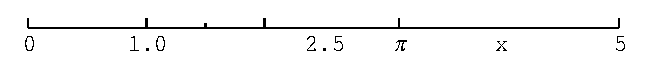
\includegraphics[width=9cm]{fig/scale.eps}
\end{minipage}\\

\hypertarget{xyname}{}
\begin{minipage}[t]{5.5cm}
xname ~''$text$''\\
yname ~''$text$''\\
\end{minipage}
\begin{minipage}[t]{9cm}
Labels $x$ and $y$ axes.
$text$ should be inside quote.
Inside $text$, \TeX commands can be used.
Also, characters such as those that can be obtained
with \TeX can be written with this command.
\end{minipage}\\

\begin{minipage}[t]{5.5cm}
 print ~x ~y ~''$text$'' [$th$]\\
 printc ~x ~y ~''$text$'' [$th$]
\end{minipage}
\begin{minipage}[t]{9cm}
This command writes $text$ in the assigned position (x ~y).
The option $th$ assigned the rotation degree.

\begin{tabular}{cc}
\includegraphics{fig/fig-print1.eps}&  
\includegraphics{fig/fig-print2.eps}\\
print&printc
\end{tabular}p
\end{minipage}\\

\begin{minipage}[t]{5.5cm}
title ~x ~y ~''$text$'' [$th$]\\
titlec ~x ~y ~''$text$'' [$th$]
\end{minipage}
\begin{minipage}[t]{9cm}
This command is same as print(c).
However, the basic unit is expressed in absolute value mm.
The reference point is on the bottom-left.
\end{minipage}\\

\begin{minipage}[t]{5.5cm}
csize ~h [w]
\end{minipage}
\begin{minipage}[t]{9cm}
This command assigns in mm the character width and height,
to be used in the following commands:\\
x/yscale, x/yname, print/c, title/c\\
When the value of $w$ is omitted, $w$ is made equal to $h$.
The default values for the option --{\bf s} follows:
\begin{tabular}{ccc}

--{\bf s} &w &h  \\ \hline
1 &2.5 &2.2\\
2&5&2.6\\
3&2.5&4.4\\
4&5&4.4
\end{tabular}\\

\end{minipage}\\

\begin{minipage}[t]{5.5cm}
 pen ~$penno$
\end{minipage}
\begin{minipage}[t]{9cm}
This command chooses the variable $penno$.
$1 \leq  penno \leq 10$
Please refer to \hyperlink{pen-color}{appendix}.
\end{minipage}\\

\begin{minipage}[t]{5.5cm}
 join ~$joinno$
\end{minipage}
\begin{minipage}[t]{9cm}
This command chooses the variable $joinno$.
$0 \leq joinno \leq 2$
Please refer to the \hyperlink{join-type}{appendix}.
\end{minipage}\\

\begin{minipage}[t]{5.5cm}
line ~$ltype$ [$lpt$]
\end{minipage}
\begin{minipage}[t]{9cm}
This command assigns the type $ltype$ of the line which will connect
data as well as the $lpt$ pace. $lpt$ is on mm unit.
When $ltype$=0: no line is used to connect coordinate points.
1:~solid~~2:~dotted~~3:~dot and dash~~4:~broken~~5:~dash
Please refer to the \hyperlink{pen-line}{appendix}.\\
        
\end{minipage}\\

\begin{minipage}[t]{5.5cm}
xgrid ~$x_1$ ~$x_2$ ~$\dots$\\
ygrid ~$y_1$ ~$y_2$ ~$\dots$
\end{minipage}
\begin{minipage}[t]{9cm}
This command makes grids in the positions $x_1$ $x_2$ $\dots$,
$y_1$ $y_2$ $\dots$.\\
(Example)\\
\begin{minipage}[t]{4.3cm}
 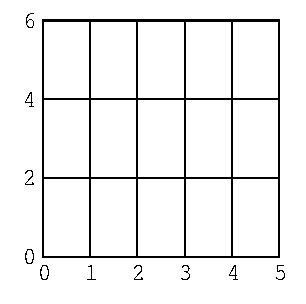
\includegraphics[width=4cm]{fig/grid.eps}
\end{minipage}
\begin{minipage}[b]{4.5cm}
\baselineskip 5pt
x 0 5\\
y 0 6\\
xscale 0 1 2 3 4 5\\
yscale 0 2 4 6

\vspace{3mm}
xgrid 1 2 3 4\\
ygrid 2 4
\vspace*{1cm}
\end{minipage}
\end{minipage}\\


\begin{minipage}[t]{5.5cm}
mark ~$label$ [$th$]
\end{minipage}
\begin{minipage}[t]{9cm}
This command draws a mark in the assigned coordinate position.
The option $th$ assigns angle(degree) that the string will be draw.
If $label$ is assigned $\backslash 0$, the mark is released.
The way to write marks and special characters can be seen
at the $label$ section of data explanation.
\end{minipage}\\

\begin{minipage}[t]{5.5cm}
hight ~$h$ [$w$]\\
italic ~$th$
\end{minipage}
\begin{minipage}[t]{9cm}
This command defines the size of the label through its
height $h$(mm) and width $w$(mm) whenever it is assigned
and allows for writing a label in italic.
\end{minipage}\\

\begin{minipage}[t]{5.5cm}
circle ~x ~y ~$r_1$ ~$r_2$ ~$\dots$\\
xcircle ~x ~y ~$r_1$ ~$r_2$ ~$\dots$\\
ycircle ~x ~y ~$r_1$ ~$r_2$ ~$\dots$

\end{minipage}
\begin{minipage}[t]{9cm}
This command writes a circle with radius $r_1$ ~$r_2$ ~$\dots$
with center on the coordinate ($x$,~$y$).
Also, the unit for the radius $r_x$ in the circle command is mm,
for the xcircle command is the scale of the $x$ axis and
for the ycircle command is the scale of the $y$ axis,
as can be seen in the figure below.\\
(Example)\\
\begin{minipage}[t]{4.3cm}
 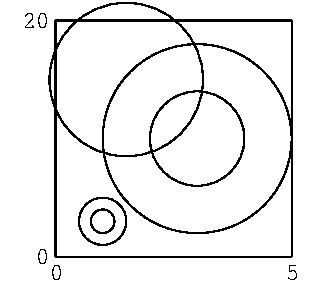
\includegraphics[width=4cm]{fig/circle.eps}
\end{minipage}
\begin{minipage}[b]{4.5cm}
\baselineskip 5pt
x 0 5\\
y 0 20\\
xscale 0 5\\
yscale 0 20

\vspace*{3mm}
xcircle 3 10 1 2\\
ycircle 1 3 1 2\\
circle  1.5 15 13\\
\vspace*{7mm}
\end{minipage}
\end{minipage}\\

\begin{minipage}[t]{5.5cm}
box ~$x_0$ $y_0$ $x_1$ ~$y_1$ [~$x_2$ $y_2$ $\dots$ ]\\
paint ~$type$
\end{minipage}
\begin{minipage}[t]{9cm}
This command draws a rectangle with paint $type$
connecting ($x_0$ $y_0$) and ($x_1$ $y_1$) through a solid line.
The line which connects ($x_0$ $y_0$) and ($x_1$ $y_1$) forms
a diagonal of the rectangle.
Also, if $x_2$ $y_2$ $\dots$ are assigned, a polygon is draw connecting
($x_0$ $y_0$),($x_1$ $y_1$),($x_2$ $y_2$),$\dots$.
In this case, Please do not use paint $type$ different from 1.
The default of paint is 1.\\

(Example)\\
\begin{minipage}[t]{4.3cm}
 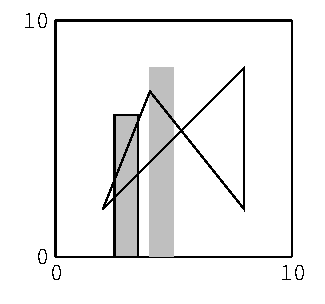
\includegraphics[width=4cm]{fig/box.eps}
\end{minipage}
\begin{minipage}[b]{4.5cm}
\baselineskip 5pt
x 0 10\\
y 0 10\\
xscale 0 10\\
yscale 0 10

\vspace*{3mm}
paint 18\\
box 2.5 0 3.5 6\\
paint -18 \\
box 4 0 5 8\\
paint 1\\
box  2 2 8 8 8 2 4 7
\end{minipage}
\end{minipage}\\

\begin{minipage}[t]{5.5cm}
clip ~$x_0$ $y_0$ $x_1$ ~$y_1$ 
\end{minipage}
\begin{minipage}[t]{9cm}
This command allows for drawing only inside the box defined by
($x_0$ $y_0$), ($x_1$ $y_1$).
When the coordinates ($x_0$ $y_0$), ($x_1$ $y_1$) are omitted,
then the clip command is released.\\

(Example)\\
\begin{minipage}[t]{4.3cm}
 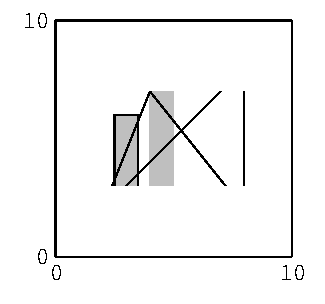
\includegraphics[width=4cm]{fig/clip.eps}
\end{minipage}
\begin{minipage}[b]{4.5cm}
\baselineskip 5pt
x 0 10\\
y 0 10\\
xscale 0 10\\
yscale 0 10

\vspace*{3mm}
clip 2 3 9 7\\
paint 18\\
box 2.5 0 3.5 6\\
paint -18 \\
box 4 0 5 8\\
paint 1\\
box  2 2 8 8 8 2 4 7
\end{minipage}
\end{minipage}\\

\begin{minipage}[t]{5.5cm}
\# any comment
\end{minipage}
\begin{minipage}[t]{9cm}
This is used for comment lines.
Whatever is written after this symbol
is ignored by the fig command.
\end{minipage}\\
\end{qsection}

\begin{qsection}{\ ~~~DATA LINES}
\begin{minipage}[t]{5.5cm}
 x ~y [$label$~ [$th$]]
\end{minipage}
\begin{minipage}[t]{9cm}
The coordinates (x ~y) are scaled by the values assigned in the
command lines.
If a string is written on $label$, then it will be written
in the (x ~y) position.
No empty character (e.g., space character) should be left in $label$.
When $label$ is assigned in mark command,
$label$ replacement will take place only for this coordinate.
The option $th$ assigns the angle.\\
If $\backslash n$, where $0 \leq n \leq 15$, is assigned to $label$,
the corresponding mark is draw (refer to the \hyperlink{lmark}{appendix} for the types of
marks).
When a minus sign is written before mark number,
then the connecting line between marks passes through the center of
each mark.\\
If a minus sign is not included, then connecting lines do not pass
through the center of each mark.
When $n=16(\backslash 16)$, a small circle is written with
diameter defined by the hight command.
Also, special character and ASCII character can be written through
code number when $n>32$.
\end{minipage}\\

\begin{minipage}[t]{5.5cm}
 eod\\
EOD
\end{minipage}
\begin{minipage}[t]{9cm}
This is the end of data sign.
Coordinates before and after the eod sign are not connected.
\end{minipage}
\end{qsection}
\newpage
\begin{qsection}{APPENDIX}
\hypertarget{lmark}{}
{\large \hspace{-1.5ex}$\bullet$
The following type of marks can be defined through $label$:}

\begin{center}
\leavevmode
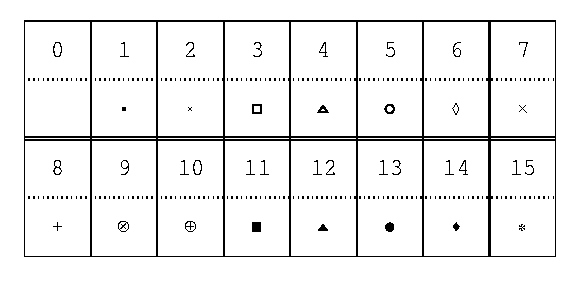
\includegraphics[width=12cm]{fig/mark.eps} \\
\end{center}

\hypertarget{pen-line}{}
{\large \hspace{-1.5ex}$\bullet$
The following types of pen and line can be defined:}\\
\hspace{3mm}[When output is obtained through the command \hyperlink{psgr}{psgr}]

\leavevmode
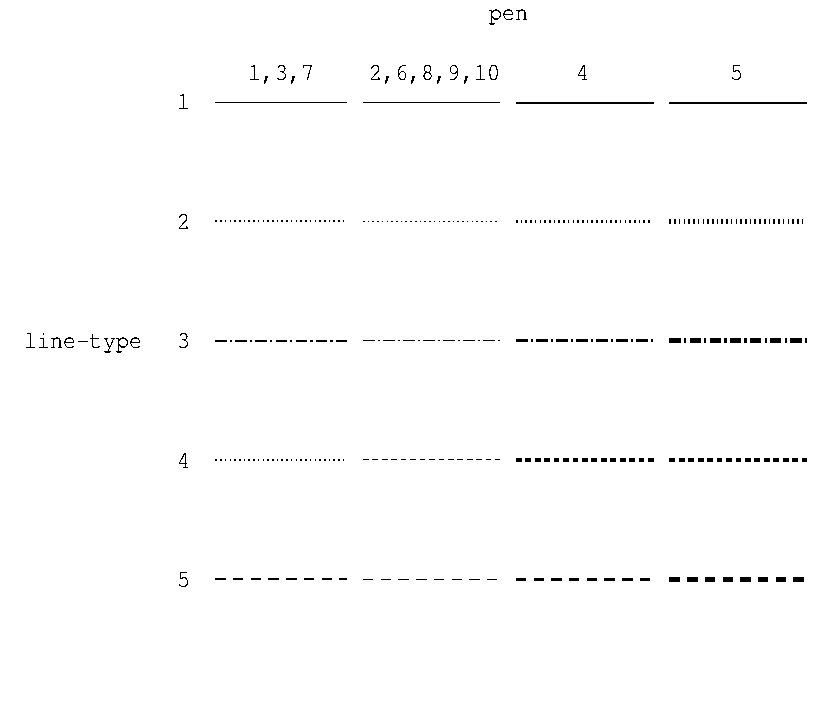
\includegraphics{fig/pen-line.eps} \\

(Attention)~~ The types of output generate through the pen command
depends on the printer (Please try printing this page).
\newpage
[When output is obtained through the command \hyperlink{xgr}{xgr}]\\
\hypertarget{pen-color}{}
The following colors can be used.\\

\begin{center}
\begin{tabular}{|c|c|c|c|c|c|c|c|c|c|c|}
 \hline
 pen type& 1& 2& 3& 4& 5& 6& 7& 8& 9&10  \\ \hline
 color   & black& blue& red& green& pink& orange& emerald& gray&brown & 
 dark blue \\ \hline
\end{tabular}\\
\end{center}

\vspace{5mm}
\hypertarget{join-type}{}
{\large \hspace{-1.5ex}$\bullet$ 
The following types of joins can be defined:}\\
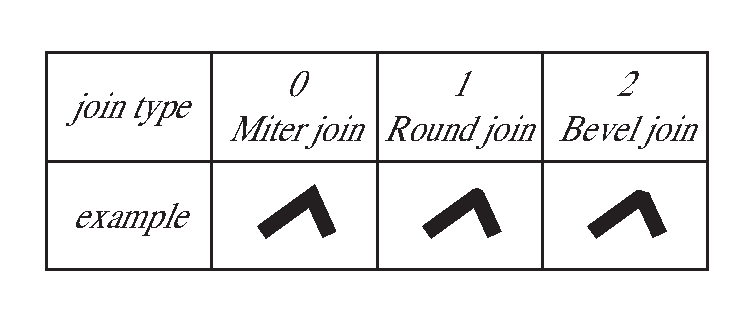
\includegraphics[width=9cm]{fig/join-type.eps}\\

\vspace{5mm}
{\large \hspace{-1.5ex}$\bullet$ paint type:}\\
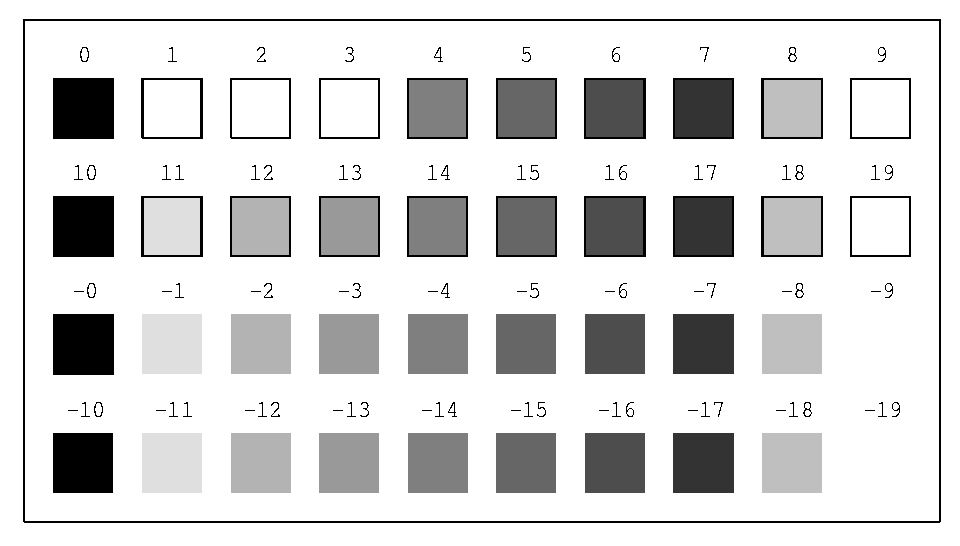
\includegraphics{fig/paint.eps}\\
(Attention)~~~From $1 \sim 3$ only a frame is draw,
and for $-9$ and $-19$ the center is white and no frame is draw.

\end{qsection}

% ----------------------------------------------------------------- %
%             The Speech Signal Processing Toolkit (SPTK)           %
%             developed by SPTK Working Group                       %
%             http://sp-tk.sourceforge.net/                         %
% ----------------------------------------------------------------- %
%                                                                   %
%  Copyright (c) 1984-2007  Tokyo Institute of Technology           %
%                           Interdisciplinary Graduate School of    %
%                           Science and Engineering                 %
%                                                                   %
%                1996-2015  Nagoya Institute of Technology          %
%                           Department of Computer Science          %
%                                                                   %
% All rights reserved.                                              %
%                                                                   %
% Redistribution and use in source and binary forms, with or        %
% without modification, are permitted provided that the following   %
% conditions are met:                                               %
%                                                                   %
% - Redistributions of source code must retain the above copyright  %
%   notice, this list of conditions and the following disclaimer.   %
% - Redistributions in binary form must reproduce the above         %
%   copyright notice, this list of conditions and the following     %
%   disclaimer in the documentation and/or other materials provided %
%   with the distribution.                                          %
% - Neither the name of the SPTK working group nor the names of its %
%   contributors may be used to endorse or promote products derived %
%   from this software without specific prior written permission.   %
%                                                                   %
% THIS SOFTWARE IS PROVIDED BY THE COPYRIGHT HOLDERS AND            %
% CONTRIBUTORS "AS IS" AND ANY EXPRESS OR IMPLIED WARRANTIES,       %
% INCLUDING, BUT NOT LIMITED TO, THE IMPLIED WARRANTIES OF          %
% MERCHANTABILITY AND FITNESS FOR A PARTICULAR PURPOSE ARE          %
% DISCLAIMED. IN NO EVENT SHALL THE COPYRIGHT OWNER OR CONTRIBUTORS %
% BE LIABLE FOR ANY DIRECT, INDIRECT, INCIDENTAL, SPECIAL,          %
% EXEMPLARY, OR CONSEQUENTIAL DAMAGES (INCLUDING, BUT NOT LIMITED   %
% TO, PROCUREMENT OF SUBSTITUTE GOODS OR SERVICES; LOSS OF USE,     %
% DATA, OR PROFITS; OR BUSINESS INTERRUPTION) HOWEVER CAUSED AND ON %
% ANY THEORY OF LIABILITY, WHETHER IN CONTRACT, STRICT LIABILITY,   %
% OR TORT (INCLUDING NEGLIGENCE OR OTHERWISE) ARISING IN ANY WAY    %
% OUT OF THE USE OF THIS SOFTWARE, EVEN IF ADVISED OF THE           %
% POSSIBILITY OF SUCH DAMAGE.                                       %
% ----------------------------------------------------------------- %
\hypertarget{frame}{}
\name{frame}{extract frame from data sequence}{signal processing,speech analysis and synthesis}

\begin{synopsis}
 \item [frame] [ --l $L$ ] [ --n ] [ --p $P$ ] [ {\em infile} ]
\end{synopsis}

\begin{qsection}{DESCRIPTION}
{\em frame} converts a sequence of input data 
from {\em infile} (or standard input) 
to a series of possibly-overlapping frames with period $P$ and length $L$, 
and sends the result to standard output.
If the input data is $x(0),x(1),\ldots,x(T)$, then the output data
 will be given by :
\begin{center}
\begin{tabular}{ccccccccccc}
$0$&$,$&$0$&$,$&$\ldots$&$,$&$x(0)$&$,$&$\ldots$&$,$&$x(L/2)$\\
$x(P-L/2)$&$,$&$x(P-L/2+1)$&$,$&$\ldots$&$,$&$x(P)$&$,$&$\ldots$&$,$&$x(P+L/2)$\\
$x(2P-L/2)$&$,$&$x(2P-L/2+1)$&$,$&$\ldots$&$,$&$x(2P)$&$,$&$\ldots$&$,$&$x(2P+L/2)$\\
&&&&&&$\vdots$&&&&
\end{tabular}
\end{center}

\end{qsection}

\begin{options}
	\argm{l}{L}{frame length}{256}
	\argm{p}{P}{frame period}{100}
	\argm{n}{}{This option is used when, instead of having x(0) as the
                   center point in the first frame, one want to make x(0)
                   as the first point of the first frame}{FALSE}
\end{options}


\begin{qsection}{EXAMPLE}
In the example below, data is read from {\em data.f} file.  The frame length and
frame period are of 400 and 80, respectively, and Blackman window is used. Moreover,
linear prediction analysis is applied. The output is written in {\em data.lpc} file:
\begin{quote}
 \verb!frame -l 400 -p 80 < data.f | window -l 400 | \!\\
 \verb!lpc > data.lpc!
\end{quote}
\end{qsection}

\begin{qsection}{SEE ALSO}
\hyperlink{bcp}{bcp},
\hyperlink{x2x}{x2x},
\hyperlink{bcut}{bcut},
\hyperlink{window}{window}
\end{qsection}

% ----------------------------------------------------------------- %
%             The Speech Signal Processing Toolkit (SPTK)           %
%             developed by SPTK Working Group                       %
%             http://sp-tk.sourceforge.net/                         %
% ----------------------------------------------------------------- %
%                                                                   %
%  Copyright (c) 1984-2007  Tokyo Institute of Technology           %
%                           Interdisciplinary Graduate School of    %
%                           Science and Engineering                 %
%                                                                   %
%                1996-2013  Nagoya Institute of Technology          %
%                           Department of Computer Science          %
%                                                                   %
% All rights reserved.                                              %
%                                                                   %
% Redistribution and use in source and binary forms, with or        %
% without modification, are permitted provided that the following   %
% conditions are met:                                               %
%                                                                   %
% - Redistributions of source code must retain the above copyright  %
%   notice, this list of conditions and the following disclaimer.   %
% - Redistributions in binary form must reproduce the above         %
%   copyright notice, this list of conditions and the following     %
%   disclaimer in the documentation and/or other materials provided %
%   with the distribution.                                          %
% - Neither the name of the SPTK working group nor the names of its %
%   contributors may be used to endorse or promote products derived %
%   from this software without specific prior written permission.   %
%                                                                   %
% THIS SOFTWARE IS PROVIDED BY THE COPYRIGHT HOLDERS AND            %
% CONTRIBUTORS "AS IS" AND ANY EXPRESS OR IMPLIED WARRANTIES,       %
% INCLUDING, BUT NOT LIMITED TO, THE IMPLIED WARRANTIES OF          %
% MERCHANTABILITY AND FITNESS FOR A PARTICULAR PURPOSE ARE          %
% DISCLAIMED. IN NO EVENT SHALL THE COPYRIGHT OWNER OR CONTRIBUTORS %
% BE LIABLE FOR ANY DIRECT, INDIRECT, INCIDENTAL, SPECIAL,          %
% EXEMPLARY, OR CONSEQUENTIAL DAMAGES (INCLUDING, BUT NOT LIMITED   %
% TO, PROCUREMENT OF SUBSTITUTE GOODS OR SERVICES; LOSS OF USE,     %
% DATA, OR PROFITS; OR BUSINESS INTERRUPTION) HOWEVER CAUSED AND ON %
% ANY THEORY OF LIABILITY, WHETHER IN CONTRACT, STRICT LIABILITY,   %
% OR TORT (INCLUDING NEGLIGENCE OR OTHERWISE) ARISING IN ANY WAY    %
% OUT OF THE USE OF THIS SOFTWARE, EVEN IF ADVISED OF THE           %
% POSSIBILITY OF SUCH DAMAGE.                                       %
% ----------------------------------------------------------------- %
\hypertarget{freqt}{}
\name{freqt}{frequency transformation}%
{signal processing,speech parameter transformation}

\begin{synopsis}
\item [freqt] [ --m $M_1$ ] [ --M $M_2$ ] [ --a $A_1$ ] [ --A $A_2$ ]
	      [ {\em infile} ]
\end{synopsis}

\begin{qsection}{DESCRIPTION}
{\em freqt} converts a $M_1$-th order minimum phase sequence 
from {\em infile} (or standard input) 
into a frequency-transformed $M_2$-th order sequence,
sending the result to standard output.

Given the input sequence
\begin{displaymath}
c_{\alpha_1}(0), c_{\alpha_1}(1), \dots, c_{\alpha_1}(M_1)
\end{displaymath}
the frequency transform is given by:
\begin{displaymath}
   \alpha = (\alpha_1 - \alpha_2) / (1 - \alpha_1 \alpha_2)
\end{displaymath}
\begin{align} 
c_{\alpha_2}^{(i)}(m) &=  
	\begin{cases}
          \;\; c_{\alpha_1}(-i)
	    +\alpha\,c_{\alpha_2}^{(i-1)}(0) &  m=0 \\
          \;\; (1-\alpha^2)\,c_{\alpha_2}^{(i-1)}(0)
            +\alpha\,c_{\alpha_2}^{(i-1)}(1) &  m=1 \\
          \;\; c_{\alpha_2}^{(i-1)}(m-1) 
	    +\alpha\, \left(c_{\alpha_2}^{(i-1)}(m)
	    -c_{\alpha_2}^{(i)}(m-1)\right) &   m=2,\dots,M_2
         \end{cases} \notag \\
& \qquad\qquad\qquad\qquad\qquad\qquad i = -M_1,\dots,-1,0 
\end{align}
And the $M_2$-th order frequency transformed output sequence is of the form:
\begin{displaymath}
c_{\alpha_2}^{(0)}(0), c_{\alpha_2}^{(0)}(1), \dots, c_{\alpha_2}^{(0)}(M_2)
\end{displaymath}
\par
Input and output data are in float format.
\end{qsection}

\begin{options}
	\argm{m}{M_1}{order of minimum phase sequence}{25}
	\argm{M}{M_2}{order of warped sequence}{25}
	\argm{a}{A_1}{all-pass constant of input sequence$\alpha_1$}{0}
	\argm{A}{A_2}{all-pass constant of output sequence$\alpha_2$}{0.35}
\end{options}

\begin{qsection}{EXAMPLE}
In the following example, the linear prediction coefficients in
float format are read from {\em data.lpc} file, 
transformed in 30-th order LPC mel-cepstral coefficients,
and written in {\em data.lpcmc} file:
\begin{quote}
 \verb!lpc2c < data.lpc | freqt -m 30 > data.lpcmc!
\end{quote} 
\end{qsection}

\begin{qsection}{SEE ALSO}
\hyperlink{mgc2mgc}{mgc2mgc}
\end{qsection}

\name{gc2gc}{generalized cepstral transformation}{speech parameter convertion}

\begin{synopsis}
\item [gc2gc] [ --m $M_1$ ] [ --g $G_1$ ] [ --n ] [ --u ] 
\item [\ ~~~~~~]  [ --M $M_2$ ] [ --G $G_2$ ] [ --N ] [ --U ] [ {\em infile} ]
\end{synopsis}

\begin{qsection}{DESCRIPTION}
This command transforms a sequence of generalized cepstral coefficients
with power parameter $\gamma_1$ into generalized cepstral coefficients
with power parameter $\gamma_2$ through a regressive equation,
and writes the results to the standard output.
\par
Input and output data are in float format.
\par
The regressive equation for the generalized cepstral coefficients 
follows.
\begin{eqnarray*}
  c_{\gamma_2}(m) &=& c_{\gamma_1}(m) + \sum_{k=1}^{m-1}\frac{k}{m}
		      (\gamma_2 c_{\gamma_1}(k)c_{\gamma_2}(m-k) \nonumber\\
     		  & & \hspace{25mm} -\gamma_1 c_{\gamma_2}(k)
			c_{\gamma_1}(m-k)), ~~~m>0
\end{eqnarray*}
For the above equation, in case $\gamma_1=-1, \gamma_2=0$,
then LPC cepstral coefficients are obtained from the LPC coefficients,
in case $\gamma_1=0, \gamma_2=1$, minimum phase inpulse response is
obtained from cepstral coefficients.

If the coefficients $c_\gamma(m)$ have not been normalized,
then the input and output have following form.
\begin{displaymath}
1+\gamma c_\gamma(0), \gamma c_\gamma(1), \ldots, \gamma c_\gamma(M)
\end{displaymath}
The following applies to the case the coefficients are normalized,
\begin{displaymath}
K_\alpha,\gamma c_\gamma'(1),\ldots, \gamma c_\gamma'(M)
\end{displaymath}

\end{qsection}

\begin{options}
       -m m  :   [25]
       -g g  :   [0]
       -n    :     [FALSE]
       -u    :     [FALSE]
       -M M  :  [25]
       -G G  :  [1]
       -N    :    [FALSE]
       -U    :    [FALSE]
	\argm{m}{M_1}{order of generalized cepstrum (input)}{25}
	\argm{g}{G_1}{gamma of generalized cepstrum (input)
  	 	      If $G_1 > 1.0$ then $\gamma_1=-1 / G_1$.}{0}
	\argm{n}{}{regard input as normalized cepstrum}{FALSE}
	\argm{u}{}{regard input as multiplied by $\gamma_1$}{FALSE}
	\argm{M}{M_2}{order of generalized cepstrum (output)}{25}
	\argm{G}{G_2}{gamma of generalized cepstrum (output)
		      If $G_2 > 1.0$ then $\gamma_2=-1 / G_2$.}{1}
	\argm{N}{}{regard output as normalized cepstrum}{FALSE}
	\argm{U}{}{regard output as multiplied by $\gamma_1$}{FALSE}
\end{options}

\begin{qsection}{EXAMPLE}
In the following example, generalized cepstral coefficients
with $M=10$ and $\gamma_1=-0.5$ are read in float format from
{\em data.gcep} file, transformed into 30 order cepstral coefficients,
and written to {\em data.cep}:
\begin{quote}
 \verb!gc2gc -m 10 -g 2 -M 30 -G 0 < data.gcep > data.cep!
\end{quote} 
\end{qsection}

\begin{qsection}{SEE ALSO}
gcep, mgcep, freqt, mgc2mgc, lpc2c
\end{qsection}

\name[ref:gcep-IEICE,ref:gcep-IEEEASSP,ref:gcep-ICASSP90]{gcep}%
{$B0lHL2=%1%W%9%H%i%`J,@O(B}{$B2;@<J,@O(B}

\begin{synopsis}
\item [gcep] [ --m $M$ ] [ --g $G$ ] [ --l $L$ ] [ --n ]
	     [ --i $I$ ] [ --j $J$ ] [ --d $D$ ] [ --e $E$ ]
\item [\ ~~~~~~~] [ {\em infile} ]
\end{synopsis}

\begin{qsection}{DESCRIPTION}
$B0lHL2=%1%W%9%H%i%`J,@O$r9T$$!$(B
$B@55,2=0lHL2=%1%W%9%H%i%`(B $c_\gamma'(m)$ $B$rI8=`=PNO$K=PNO$7$^$9!%(B
$BF~NO$OAk3]$1$5$l$?D9$5(B $L$ $B$N;~7ONs(B
\begin{displaymath}
  x(0),x(1),\ldots,x(L-1)
\end{displaymath}
$B$G$9!%(B
\par
$B%G!<%?7A<0$OF~NO!$=PNO$H$b(Bfloat $B7A<0$G$9!%(B
\par
$B0lHL2=%1%W%9%H%i%`J,@O$G$O!"2;@<%9%Z%/%H%k$r(B $M$ $B<!$N0lHL2=%1%W%9%H%i%`(B 
$c_\gamma(m)$ $B$^$?$O@55,2=0lHL2=%1%W%9%H%i%`(B $c_\gamma'(m)$ $B$K$h$j(B
\begin{eqnarray*}
H(z) &=& s_\gamma^{-1}\left(
	\sum_{m=0}^{M} c_\gamma(m)z^{-m} \right) \\
     &=& K \cdot s_\gamma^{-1}\left(
	\sum_{m=1}^{M} c_\gamma'(m)z^{-m} \right) \\
     &=& \left\{ \begin{array}{ll} \displaystyle
	K\cdot \left( 1+\gamma\sum_{m=1}^{M} c_\gamma'(m)z^{-m}
		\right)^{1/\gamma}, & -1 \leq \gamma < 0 \\
	\displaystyle K\cdot \exp \sum_{m=1}^{M} c_\gamma'(m)z^{-m}, 
		& \gamma=0
	\end{array} \right.
\end{eqnarray*}
$B$H%b%G%k2=$7!$BP?t%9%Z%/%H%k$NITJP?dDjK!(B 
$B$K$*$1$kI>2A4X?t$rE,MQ$7$^$9!%(B
$BI>2A4X?t$N:G>.2=$O!"(B $\gamma=-1$ $B$N$H$-$K$O@~7AM=B,K!$G$N(B
$B@~7AJ}Dx<0$r2r$/$3$H$HEy2A$K$J$j$^$9$,!$(B
$\gamma=-1$ $B0J30$G$OHs@~7AJ}Dx<0$r2r$/$3$H$K$J$j$^$9$N$G!$(B
$B$3$3$G$O(BNewton--Raphson$BK!$rMxMQ$7$F2r$r5a$a$F$$$^$9!%(B
\end{qsection}

\begin{options}
	\argm{m}{M}{$BJ,@O<!?t!%(B}{25}
	\argm{g}{G}{$B0lHL2=%1%W%9%H%i%`$N$Y$-%Q%i%a!<%?(B $\gamma$$B!%(B\\
			 $B$?$@$7!$(B$G>1.0$ $B$N$H$-$O(B $\gamma=-1/G$$B!%(B}{0}
	\argm{l}{L}{$BF~NO%G!<%?$N%U%l!<%`D9!%(B}{256}
	\argm{n}{}{$B@55,2=$7$?%1%W%9%H%i%`$r=PNO!%(B}{FALSE}
	\desc[1zh]{$BDL>o!$0J2<$N%*%W%7%g%s$N;XDj$OI,MW$"$j$^$;$s!%(B}
	\argm{i}{I}{$BJ,@O$N:G>.H?I|2s?t!%(B}{2}
	\argm{j}{J}{$BJ,@O$N:GBgH?I|2s?t!%(B}{30}
	\argm{d}{D}{Newton-Raphson $BK!$N=*N;>r7o!%%G%U%)%k%H$O(B $D=0.001$ $B$G!$(B
		    $B$3$N$H$-$O(B $\varepsilon^{(i)}$ $B$N7+$jJV$7$K$h$kJQ2=N($,(B
		    $0.001$ $B$D$^$j(B $0.1\%$ $B0JFb$K$J$C$?$H$-$K=*N;!%(B}{0.001}
	\argm{e}{E}{$B%T%j%*%I%0%i%`$KB-$79~$`>.$5$JCM!%(B}{0}
\end{options}

\begin{qsection}{EXAMPLE}
float $B7A<0$N%U%!%$%k(B {\em data.f} $B$r<!?t(B15$B<!$G0lHL2=%1%W%9%H%i%`J,@O$7!$(B
$B0lHL2=%1%W%9%H%i%`$r(B {\em data.gcep} $B$K=PNO$9$k(B:
\begin{quote}
 \verb!frame < data.f | window | gcep -m 15 > data.gcep!
\end{quote} 
\end{qsection}

\begin{qsection}{SEE ALSO}
icep, uels, mcep, mgcep, glsadf
\end{qsection}

% ----------------------------------------------------------------
%       Speech Signal Processing Toolkit (SPTK): version 3.0
%                      SPTK Working Group
% 
%                Department of Computer Science
%                Nagoya Institute of Technology
%                             and
%   Interdisciplinary Graduate School of Science and Engineering
%                Tokyo Institute of Technology
%                   Copyright (c) 1984-2000
%                     All Rights Reserved.
% 
% Permission is hereby granted, free of charge, to use and
% distribute this software and its documentation without
% restriction, including without limitation the rights to use,
% copy, modify, merge, publish, distribute, sublicense, and/or
% sell copies of this work, and to permit persons to whom this
% work is furnished to do so, subject to the following conditions:
% 
%   1. The code must retain the above copyright notice, this list
%      of conditions and the following disclaimer.
% 
%   2. Any modifications must be clearly marked as such.
%                                                                        
% NAGOYA INSTITUTE OF TECHNOLOGY, TOKYO INSITITUTE OF TECHNOLOGY,
% SPTK WORKING GROUP, AND THE CONTRIBUTORS TO THIS WORK DISCLAIM
% ALL WARRANTIES WITH REGARD TO THIS SOFTWARE, INCLUDING ALL
% IMPLIED WARRANTIES OF MERCHANTABILITY AND FITNESS, IN NO EVENT
% SHALL NAGOYA INSTITUTE OF TECHNOLOGY, TOKYO INSITITUTE OF
% TECHNOLOGY, SPTK WORKING GROUP, NOR THE CONTRIBUTORS BE LIABLE
% FOR ANY SPECIAL, INDIRECT OR CONSEQUENTIAL DAMAGES OR ANY
% DAMAGES WHATSOEVER RESULTING FROM LOSS OF USE, DATA OR PROFITS,
% WHETHER IN AN ACTION OF CONTRACT, NEGLIGENCE OR OTHER TORTIOUS
% ACTION, ARISING OUT OF OR IN CONNECTION WITH THE USE OR
% PERFORMANCE OF THIS SOFTWARE.
% ----------------------------------------------------------------
%
\hypertarget{glogsp}{}
\name{glogsp}{draw a log spectrum graph}{plotting graphs}

\begin{synopsis}
\item[glogsp] [ --O $O$ ] [ --x $X$ ] [ --y $ymin \; ymax$ ] [ --ys $YS$ ] 
              [ --p $P$ ] [ --ln $LN$ ] 
\item[\ ~~~~~~~] [ --s $S$ ] [ --l $L$ ] [ --c $comment$ ] [ {\em infile} ]
\end{synopsis}

\begin{qsection}{DESCRIPTION}
{\em glogsp} converts float-format log spectral data 
from {\em infile} (or standard input)
to FP5301 plot format, 
sending the result to standard output. 
The output can viewed with ``xgr''.

{\em glogsp} is implemented as a shell script 
that uses the ``fig'' and ``fdrw'' commands.
\end{qsection}

\begin{options}
	\argm{O}{O}{origin of graph\\
		      \begin{minipage}{4.5cm}
		       \begin{tabular}{ccc}
			1 & ( 40,205) & [mm] \\
			2 & (125,205) & [mm] \\
			3 & ( 40,120) & [mm] \\
			4 & (125,120) & [mm] \\
			5 & ( 40, 35) & [mm] \\
			6 & (125, 35) & [mm]
		       \end{tabular}\\\hspace*{\fill}
		      \end{minipage}
		      \begin{minipage}{4.5cm}
		       \leavevmode
		       \includegraphics{fig/glogsp-on.eps}
		      \end{minipage}\\\hspace*{\fill}}{1}
	\argm{x}{X}{ $x$ scale\\
		       \begin{tabular}{cl}
			1 & normalized frequency($0 \sim 0.5$) \\
			2 & normalized frequency($0 \sim \pi$) \\
			4 & frequency($0 \sim 4$kHz) \\
			5 & frequency($0 \sim 5$kHz) \\
			8 & frequency($0 \sim 8$kHz) \\
			10 & frequency($0 \sim 10$kHz) 
		       \end{tabular}\\\hspace*{\fill}}{1}
	\argm{y}{ymin \; ymax}{ $y$ scale[dB]}{0 100}
	\argm{ys}{YS}{ Y-axis scaling factor}{20}
	\argm{p}{P}{pen number($1 \sim 10$)}{1}
	\argm{ln}{LN}{kind of line style($0 \sim 5$) please refer to ``fig''
                      command section}{1}
	\argm{s}{S}{start frame number}{0}
	\argm{l}{L}{frame length}{256}
	\argm{c}{\rm comment}{comment for the graph}{N/A}
	\desc[1ex]{Usually, the options below do not need to be assigned.}
	\argm{W}{W}{width of the graph($\time 100$mm)}{0.6}
	\argm{H}{H}{height of the graph($\time 100$mm)}{0.6}
	\argm{v}{}{over write mode}{FALSE}
	\argm{o}{xo \; yo}{origin of the graph.
                      if -o option exists, -O is not effective}{40 205}
	\argm{g}{G}{type of frame of the graph($0 \sim 2$).
                    please refer to ``fig'' command section.}{2}
	\argm{f}{file}{additional data file for fig}{NULL}
	\argm{help}{}{print help in detail}{}
\end{options}

\begin{qsection}{EXAMPLE}
In the example below, speech data sampled at 10kHz is read
in short format from {\em data.s} file,
the magnitude of its log spectrum is evaluated and plotted on the screen:
\begin{quote}
 \verb!x2x +sf data.s | bcut -s 4000 -e 4255 | window -n 2| spec |\! \\
 \verb!glogsp -x 5 | xgr!
\end{quote}
\begin{center}
 \leavevmode
 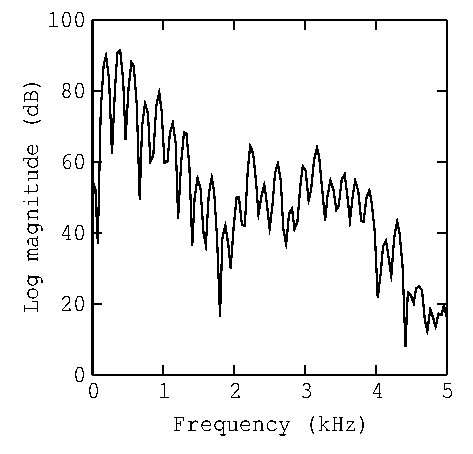
\includegraphics{fig/glogsp-sample.eps}
\end{center}
\end{qsection}

\begin{qsection}{SEE ALSO}
\hyperlink{fig}{fig},
\hyperlink{fdrw}{fdrw},
\hyperlink{xgr}{xgr},
\hyperlink{psgr}{psgr},
\hyperlink{grlogsp}{grlogsp},
\hyperlink{gwave}{gwave}
\end{qsection}


% ----------------------------------------------------------------- %
%             The Speech Signal Processing Toolkit (SPTK)           %
%             developed by SPTK Working Group                       %
%             http://sp-tk.sourceforge.net/                         %
% ----------------------------------------------------------------- %
%                                                                   %
%  Copyright (c) 1984-2007  Tokyo Institute of Technology           %
%                           Interdisciplinary Graduate School of    %
%                           Science and Engineering                 %
%                                                                   %
%                1996-2011  Nagoya Institute of Technology          %
%                           Department of Computer Science          %
%                                                                   %
% All rights reserved.                                              %
%                                                                   %
% Redistribution and use in source and binary forms, with or        %
% without modification, are permitted provided that the following   %
% conditions are met:                                               %
%                                                                   %
% - Redistributions of source code must retain the above copyright  %
%   notice, this list of conditions and the following disclaimer.   %
% - Redistributions in binary form must reproduce the above         %
%   copyright notice, this list of conditions and the following     %
%   disclaimer in the documentation and/or other materials provided %
%   with the distribution.                                          %
% - Neither the name of the SPTK working group nor the names of its %
%   contributors may be used to endorse or promote products derived %
%   from this software without specific prior written permission.   %
%                                                                   %
% THIS SOFTWARE IS PROVIDED BY THE COPYRIGHT HOLDERS AND            %
% CONTRIBUTORS "AS IS" AND ANY EXPRESS OR IMPLIED WARRANTIES,       %
% INCLUDING, BUT NOT LIMITED TO, THE IMPLIED WARRANTIES OF          %
% MERCHANTABILITY AND FITNESS FOR A PARTICULAR PURPOSE ARE          %
% DISCLAIMED. IN NO EVENT SHALL THE COPYRIGHT OWNER OR CONTRIBUTORS %
% BE LIABLE FOR ANY DIRECT, INDIRECT, INCIDENTAL, SPECIAL,          %
% EXEMPLARY, OR CONSEQUENTIAL DAMAGES (INCLUDING, BUT NOT LIMITED   %
% TO, PROCUREMENT OF SUBSTITUTE GOODS OR SERVICES; LOSS OF USE,     %
% DATA, OR PROFITS; OR BUSINESS INTERRUPTION) HOWEVER CAUSED AND ON %
% ANY THEORY OF LIABILITY, WHETHER IN CONTRACT, STRICT LIABILITY,   %
% OR TORT (INCLUDING NEGLIGENCE OR OTHERWISE) ARISING IN ANY WAY    %
% OUT OF THE USE OF THIS SOFTWARE, EVEN IF ADVISED OF THE           %
% POSSIBILITY OF SUCH DAMAGE.                                       %
% ----------------------------------------------------------------- %
\hypertarget{glsadf}{}
\name[ref:GLSA-IEICEtaikai90s]{glsadf}{GLSA digital filter for speech synthesis}%
{filters for speech synthesis}

\begin{synopsis}
\item [glsadf] [ --m $M$ ] [ --c $C$ ] [ --p $P$ ] [ --i $I$ ] [ --v ] [ --t ] [ --n ] [ --k ] [ --P $Pa$ ]
 {\em gcfile} 
\item [\ ~~~~~~~~~] [ {\em infile} ]
\end{synopsis}

\begin{qsection}{DESCRIPTION}
{\em glsadf} derives a Generalized Log Spectral Approximation digital filter 
from normalized generalized cepstral coefficients in {\em gcfile} 
and uses it to filter an excitation sequence 
from {\em infile} (or standard input) to synthesize speech data, 
sending the result to standard output.
The cepstral coefficients can be be represented as
$K,c_\gamma'(1),\dots,c_\gamma'(M)$. 

Input and output data are in float format.

The transfer function $H(z)$ are synthesis filter based on an $M$ order
normalized generalized cepstral coefficients $c_\gamma'(m)$ is 
\begin{align}
H(z) &= K \cdot D(z) \notag \\
     &= \begin{cases} \;\;\displaystyle
          K \cdot \left( 1+\gamma\sum_{m=1}^{M} c_\gamma'(m) z^{-m}
                \right)^{1/\gamma}, & 0<\gamma\leq -1 \\ 
                \;\;\displaystyle K \cdot \exp \sum_{m=1}^{M} c_\gamma'(m) z^{-m}, & \gamma=0
        \end{cases}\notag
\end{align}
In this case, we are considering only values for the power parameter
$\gamma=-1/C$, where $C$ is a natural number.
The filter $D(z)$ can be realized through a $C$ level cascade as shown
in figure\ref{fig:glsadflt_GLSA}, where
\begin{displaymath}
\frac{1}{C(z)} = \frac{1}
                {\displaystyle 1+\gamma\sum_{m=1}^{M} c_\gamma'(m) z^{-m}}
\end{displaymath}

\setcounter{figure}{0}
\begin{figure}[h]
\setlength{\unitlength}{0.3mm}
\begin{center}
\begin{picture}(300,80)(10,0)
  \thicklines
  \put(40,10){\framebox(50,40){\Large $\frac{1}{C(z)}$}}
  \put(110,10){\framebox(50,40){\Large $\frac{1}{C(z)}$}}
  \put(240,10){\framebox(50,40){\Large $\frac{1}{C(z)}$}}

  \put(10,30){\vector(1,0){30}}
  \put(90,30){\line(1,0){20}}
  \put(160,30){\line(1,0){20}}
  \put(220,30){\line(1,0){20}}
  \put(290,30){\vector(1,0){30}}

  \put(200,30){\makebox(0,0){$\cdot\cdot\cdot$}}
  \put(10,40){\makebox(0,0){Input}}
  \put(320,40){\makebox(0,0){Output}}
  \put(60,65){\makebox(0,0){\bf level 1}}
  \put(140,65){\makebox(0,0){\bf level 2}}
  \put(270,65){\makebox(0,0){\bf level $C$}}

\end{picture}
\caption{Structure of filter $D(z)$}
\label{fig:glsadflt_GLSA}
\end{center}
\end{figure}
\end{qsection}

\newpage
\begin{options}
        \argm{m}{M}{order of generalized cepstrum}{25}
        \argm{c}{C}{power parameter $\gamma=-1/C$ for generalized cepstrum\\
                         if $C==0$ then the LMA filter is used}{1}
        \argm{p}{P}{frame period}{100}
        \argm{i}{I}{interpolation period}{1}
        \argm{n}{}{regard input as normalized generalized cepstrum}{FALSE}
        \argm{v}{}{inverse filter}{FALSE}
        \argm{t}{}{transpose filter}{FALSE}
        \argm{k}{}{filtering without gain}{FALSE}
        \desc[1ex]{The option below only works if $C==0$.}
        \argm{P}{Pa}{order of the Pad\'e approximation\\
                     $Pa$ should be $4$ or $5$}{4}
\end{options}

\begin{qsection}{EXAMPLE}
In this example, excitation is generated through the pitch data
in the file {\em data.pitch} in float format, passed through a
GLSA filter based on the generalized cepstral coefficients file
{\em data.gcep}, and the synthesized speech is output to
{\em data.syn}:
\begin{quote}
 \verb!excite < data.pitch | glsadf data.gcep > data.syn!
\end{quote} 
\end{qsection}

\begin{qsection}{SEE ALSO}
\hyperlink{ltcdf}{ltcdf},
\hyperlink{lmadf}{lmadf},
\hyperlink{lspdf}{lspdf},
\hyperlink{mlsadf}{mlsadf},
\hyperlink{mglsadf}{mglsadf}
\end{qsection}

% ----------------------------------------------------------------- %
%             The Speech Signal Processing Toolkit (SPTK)           %
%             developed by SPTK Working Group                       %
%             http://sp-tk.sourceforge.net/                         %
% ----------------------------------------------------------------- %
%                                                                   %
%  Copyright (c) 1984-2007  Tokyo Institute of Technology           %
%                           Interdisciplinary Graduate School of    %
%                           Science and Engineering                 %
%                                                                   %
%                1996-2015  Nagoya Institute of Technology          %
%                           Department of Computer Science          %
%                                                                   %
% All rights reserved.                                              %
%                                                                   %
% Redistribution and use in source and binary forms, with or        %
% without modification, are permitted provided that the following   %
% conditions are met:                                               %
%                                                                   %
% - Redistributions of source code must retain the above copyright  %
%   notice, this list of conditions and the following disclaimer.   %
% - Redistributions in binary form must reproduce the above         %
%   copyright notice, this list of conditions and the following     %
%   disclaimer in the documentation and/or other materials provided %
%   with the distribution.                                          %
% - Neither the name of the SPTK working group nor the names of its %
%   contributors may be used to endorse or promote products derived %
%   from this software without specific prior written permission.   %
%                                                                   %
% THIS SOFTWARE IS PROVIDED BY THE COPYRIGHT HOLDERS AND            %
% CONTRIBUTORS "AS IS" AND ANY EXPRESS OR IMPLIED WARRANTIES,       %
% INCLUDING, BUT NOT LIMITED TO, THE IMPLIED WARRANTIES OF          %
% MERCHANTABILITY AND FITNESS FOR A PARTICULAR PURPOSE ARE          %
% DISCLAIMED. IN NO EVENT SHALL THE COPYRIGHT OWNER OR CONTRIBUTORS %
% BE LIABLE FOR ANY DIRECT, INDIRECT, INCIDENTAL, SPECIAL,          %
% EXEMPLARY, OR CONSEQUENTIAL DAMAGES (INCLUDING, BUT NOT LIMITED   %
% TO, PROCUREMENT OF SUBSTITUTE GOODS OR SERVICES; LOSS OF USE,     %
% DATA, OR PROFITS; OR BUSINESS INTERRUPTION) HOWEVER CAUSED AND ON %
% ANY THEORY OF LIABILITY, WHETHER IN CONTRACT, STRICT LIABILITY,   %
% OR TORT (INCLUDING NEGLIGENCE OR OTHERWISE) ARISING IN ANY WAY    %
% OUT OF THE USE OF THIS SOFTWARE, EVEN IF ADVISED OF THE           %
% POSSIBILITY OF SUCH DAMAGE.                                       %
% ----------------------------------------------------------------- %
\hypertarget{gmm}{}
\name[ref:GMMMAP-IEEE]{gmm}{GMM parameter estimation}{model training}

\begin{synopsis}
\item [gmm] [ --l $L$ ] [ --m $M$ ] [ --t $T$ ] [ --s $S$ ] [ --a $A$ ] [ --b $B$ ]
        [ --e $E$ ] [ --v $V$ ] [ --w $W$ ] [ --f ]
\item [\ ~~~~]  [ --M $W_{MAP}$ ][ --F $gmmfile$ ] [ --B $B1,B2,...$ ] [ --c1 ] [ --c2 ] [ {\em infile} ]
\end{synopsis}

\newfont{\bggg}{cmr10 scaled\magstep3}
\newcommand{\bigzerol}{\smash{\hbox{\bggg 0}}}
\newcommand{\bigzerou}{\smash{\lower1.3ex\hbox{\bggg 0}}}
\newcommand{\argmax}{\mathop{\rm argmax}\limits}

\begin{qsection}{DESCRIPTION}
{\em gmm} uses the expectation maximization (EM) algorithm to estimate
Gaussian mixture model (GMM) parameters with diagonal covariance
matrices, from a sequence of vectors in the {\em infile} (or standard
input), sending the result to standard output.

The input sequence $\bX$ consists of $T$ float vectors $\bx$, each of
size $L$:
\begin{align}
 &\bX=\left[\bx(0), \bx(1), \dots, \bx(T-1)\right]\notag,\\
 &\bx(t)=\left[x_t(0), x_t(1), \ldots, x_t(L-1)\right].\notag
\end{align}
The result is GMM parameters $\lambda$ consisting of $M$ mixture weights
$\bw$ and $M$ Gaussians with mean vector $\bmu$ and variance vector
$\bv$, each of length $L$:
\begin{align}
 \lambda =
 \left[\bw,\right.&\left.\bmu(0),\bv(0), \bmu(1), \bv(1),
 \ldots, \bmu(M-1), \bv(M-1)\right],\notag\\[2mm]
 \bw &=\left[ w(0), w(1), \ldots, w(M-1) \right],\notag\\
 \bmu(m) &=\left[\mu_m(0), \mu_m(1), \ldots, \mu_m(L-1)\right],\notag\\
 \bv(m) &=\left[\sigma_m^2(0), \sigma_m^2(1), \ldots,
 \sigma_m^2(L-1)\right],\notag
\end{align}
where
\begin{displaymath}
 \sum_{m=0}^{M-1}w(m)=1.
\end{displaymath}

The GMM parameter set $\lambda$ is initialized by an LBG algorithm and
the following EM steps are used iteratively to obtain the new parameter set
$\hat{\lambda}$:
\begin{align}
   \hat{w}(m) & = \frac{1}{T}
   \sum_{t=0}^{T-1}p(m\mid\bx(t),\lambda),\notag\\
  \hat{\bmu}(m) & 
 = \frac{\sum_{t=0}^{T-1}p(m\mid\bx(t),\lambda)\bx(t)}
 {\sum_{t=0}^{T-1}p(m\mid\bx(t),\lambda)}, \notag\\[2mm]
  \hat{\sigma}_m^2(l)&
  =\frac{\sum_{t=0}^{T-1}p(m\mid\bx(t),\lambda)x_t^2(l)}
  {\sum_{t=0}^{T-1}p(m\mid\bx(t),\lambda)}
 - \hat{\mu}_m^2(l),\notag
\end{align}
where $p(m\mid\bx(t),\lambda)$ is the posterior probability of being in
the $m$-th component at time $t$ and is given by:
\begin{displaymath}
 p(m\mid\bx(t),\lambda)
 = \frac{w(m){\cal N}(\bx(t)\mid \bmu(m),\bv(m))}
 {\sum_{k=0}^{M-1}w(k){\cal N}(\bx(t)\mid \bmu(k),\bv(k))},
\end{displaymath}
 where
\begin{align}
 {\cal N}(\bx(t)\mid\bmu(m),\bv(m))%
 &=\frac{1}{(2\pi)^{L/2}\,|\Sigma(m)|^{1/2}}%
 \exp{\left\{-\frac{1}{2}%
 (\bx(t)-\bmu(m))'\,\Sigma(m)^{-1}\,%
 (\bx(t)-\bmu(m))\right\}}\notag\\
 &=\frac{1}{(2\pi)^{L/2}\prod_{l=0}^{L-1}\sigma_m(l)}%
 \exp{\left\{-\frac{1}{2}%
 \sum_{l=0}^{L-1}
 \frac{\left(x_t(l)-\mu_m(l)\right)^2}%
 {\sigma_m^2(l)}\right\}},\notag
\end{align}
and $\Sigma(m)$ is a diagonal matrix with diagonal elements
 $\bv(m)$:
\begin{displaymath}
 \Sigma(m)=\left[
 \begin{array}{cccc}
  \sigma_m^2(0) & & &\bigzerou\\
  & \sigma_m^2(1) & &\\
  & & \ddots &\\
  \bigzerol & & & \sigma_m^2(L-1)\\
 \end{array}\right].\notag
\end{displaymath}

Also, the Average log-likelihood for training data $X$
\begin{displaymath}
  \log p(\bX | \lambda)
 =\frac{1}{T}\sum_{t=0}^{T-1}
 \log\sum_{m=0}^{M-1}w(m){\cal N}(\bx(t)\mid\bmu(m),\bv(m))
\end{displaymath}
is increased by iterating the above steps. The average log-probability $\log
p(\bX|\lambda)$ at each iterative step is printed on the standard error output.
The EM steps are iterated at least $A$ times and stopped at the $B$-th
iteration or when there is a small absolute change in $\log p(\bX|\lambda)~(\leq
E)$.

If the -M option is specified, {\em gmm} estimates parameters using Maximum a Posteriori (MAP) method. The parameters $\lambda_{MAP}$ are defined as the mode of the posterior probability density function of $\lambda$ denoted as $p(\lambda|\bX)$, i.e.
\begin{align}
 \lambda_{MAP} &= \argmax_{\lambda} p(\lambda | \bX) \notag \\
               &= \argmax_{\lambda} p(\bX | \lambda) p(\lambda). \notag
\end{align}
The joint prior density $p(\lambda)$ is the product of Dirichlet and normal-Wishart densities as follows:
\begin{displaymath}
 p(\lambda) = g(w(0),\cdots,w(M-1))\prod^{M-1}_{m=0} g(\bmu(m),\bnu(m))
\end{displaymath}
where 
\begin{align}
 &g(w(0),\cdots,w(M-1)|\beta(0),\cdots,\beta(M-1)) \propto \prod^{M-1}_{m=0} w(m)^{\beta(m)-1} \, , \notag \\
 &g(\bmu(m),\bnu(m)|\tau(m),\bmu'(m),\alpha(m),\bu(m)) \propto \mid \bSigma(m) \mid^{-\frac{\alpha(m)-L}{2}} \notag \\
 &\cdot \exp \left\{ -\frac{\tau(m)}{2}(\bmu(m)-\bmu'(m))^\top \bSigma(m)^{-1} (\bmu(m)-\bmu'(m)) \right\} \exp \left\{ -\frac{1}{2}\mathrm{Tr}\left( \bu(m) \bSigma(m)^{-1} \right) \right\}. \notag
\end{align}
Then the updated parameters are derived from:
\begin{align}
 \hat{w}(m)&=\frac{(\beta(m)-1)+\sum^{T-1}_{t=0}c_{mt}}{\sum^{M-1}_{m=0}(\beta(m)-1) + \sum^{M-1}_{m=0}\sum^{T-1}_{t=0}c_{mt}} \, ,\notag \\
 \hat{\bmu}(m)&=\frac{\tau(m)\bmu'(m)+\sum^{T-1}_{t=0}c_{mt}\bx(t)}{\tau(m)+\sum^{T-1}_{t=0}c_{mt}} \, ,\notag \\
 \hat{\bSigma}(m)&=\frac{\bu(m)+\sum^{T-1}_{t=0}c_{mt}(\bx(t)-\hat{\bmu}(m))(\bx(t)-\hat{\bmu}(m))^\top + \tau(m)(\bmu'(m)-\hat{\bmu}(m))(\bmu'(m)-\hat{\bmu}(m))^\top}{(\alpha(m)-L) + \sum^{T-1}_{t=0}c_{mt}} \, . \notag
\end{align}
where
\begin{align}
 c_{mt} &= p(m|\bx(t),\lambda) \, , \notag \\
 \beta(m)-1 &= \tau(m) = W_{MAP} w'(m) \, , \notag \\ 
 \alpha(m) &= \tau(m) + L \notag \, , \\
 \bu(m) &= \tau(m) \bSigma'(m) \, . \notag
\end{align}
The parameters 
 \begin{displaymath}
  \lambda'=(w'(0),\cdots,w'(M-1), \bmu'(0),\cdots,\bmu'(M-1), \bnu'(0),\cdots,\bnu'(M-1))
 \end{displaymath}
are obtained from the pre-estimated universal background model (UBM).
\end{qsection}

\begin{options}
 \argm{l}{L}{length of vector}{26}
 \argm{m}{M}{number of Gaussian components}{16}
 \argm{t}{T}{number of training vectors}{N/A}
 \argm{s}{S}{seed of random variable for LBG algorithm}{1}
 \argm{a}{A}{minimum number of EM iterations}{0}
 \argm{b}{B}{maximum number of EM iterations (A$\leq$ B)}{20}
 \argm{e}{E}{end condition for EM iteration}{0.00001}
 \argm{v}{V}{flooring value for variances}{0.001}
 \argm{w}{W}{flooring value for weights (1/M)*W}{0.001}
 \argm{f}{}{full covariance}{FALSE}
 \argm{M}{W_{MAP}}{using maximum a posteriori(MAP) estimation,\\
                             where $W_{MAP}$ is the parameter for\\
                             Dirichlet and normal-Wishart densities.}{0.0}
 \argm{F}{fn}{GMM initial parameter file\\
                             If -M option is specified,\\
                             fn is regarded as the parameter for UBM.}{N/A}
 \desc[1ex]{(level 2)}
 \argm{B}{B1~B2~$\ldots$~Bn}{block size in covariance matrix,\\
                             where $(B1+B2+\ldots+Bn)=L$}{N/A}
 \argm{c1}{}{inter-block correlation}{N/A}
 \argm{c2}{}{full covariance in each block}{N/A}
\end{options}

\begin{qsection}{EXAMPLE}
In the following example, a GMM with 8 Gaussian components is generated
from training vectors {\em data.f} in float format, and GMM parameters
are written to {\em gmm.f}.
\begin{quote}
\verb! gmm -m 8 data.f > gmm.f!
\end{quote}
If one wants to model GMMs with full covariances,
 one can use the -f option.
\begin{quote}
\verb! gmm -m 8 -f data.f > gmm.f! 
\end{quote}
The -F option can be used to specify GMM
initial parameter file {\em gmm.init}.
\begin{quote}
\verb! gmm -m 8 -f data.f -F gmm.init > gmm.f! 
\end{quote}

If the -M option is specified as follows, the MAP estimates of the GMM parameters {\em map.gmm} are obtained using universal background model {\em ubm.gmm}.
\begin{quote}
 \verb! gmm -l 15 -m 8 -M 1.0 -F ubm.gmm data.f > map.gmm !
\end{quote}

In the followings, 15-dimentional training vectors {\em data.f} can be modeled
by a GMM with 8 Gaussian components.  If one wants to divide the covariance
matrix into several blocks, the -B option can be used to specify size of each
blocks in covariance matrix.  For example, when dividing 15-dimentional vector
into 3 sub-parts, where each part has 5 dimention, the structure of the
covariance matrix can be represented by $3 \times 3$ sub-blocks:
 \begin{quote}
  \verb! gmm -l 15 -m 8 data.f -B 5 5 5 > gmm.f!
 \end{quote}
 Note that without -c1 and -c2 option, a diagonal covariance can be obtained
 as shown in figure \ref{fig:gmm_c1} (a).
 An example of the corresponding structure of
 the covariance matrix is shown in figure \ref{fig:gmm_c1} (a).

 If one wants to turn on inter-block correlation,
 The -c1 option can be used and corresponding command line is below.
 \begin{quote}
  \verb! gmm -l 15 -m 8 data.f -B 5 5 5 -c1 > gmm.f!
 \end{quote}
 The corresponding example is shown in figure \ref{fig:gmm_c1} (b).

 If one wants to turn on block-wise full covariance,
 The -c2 option can be used and the corresponding command line is below.
 \begin{quote}
  \verb! gmm -l 15 -m 8 data.f -B 5 5 5 -c2 > gmm.f!
 \end{quote}
 The corresponding example is shown in figure \ref{fig:gmm_c1} (c).

 By specifying both -c1 and -c2 option, a full covariance matrix
 can be obtained as shown in figure \ref{fig:gmm_c1} (d).
 This case is equivalent to the case that only -f option is specified.
 \begin{figure}[h]
 \begin{center}
  \begin{tabular}{cc}
   \begin{minipage}[b]{0.45\hsize}
     \begin{center}
      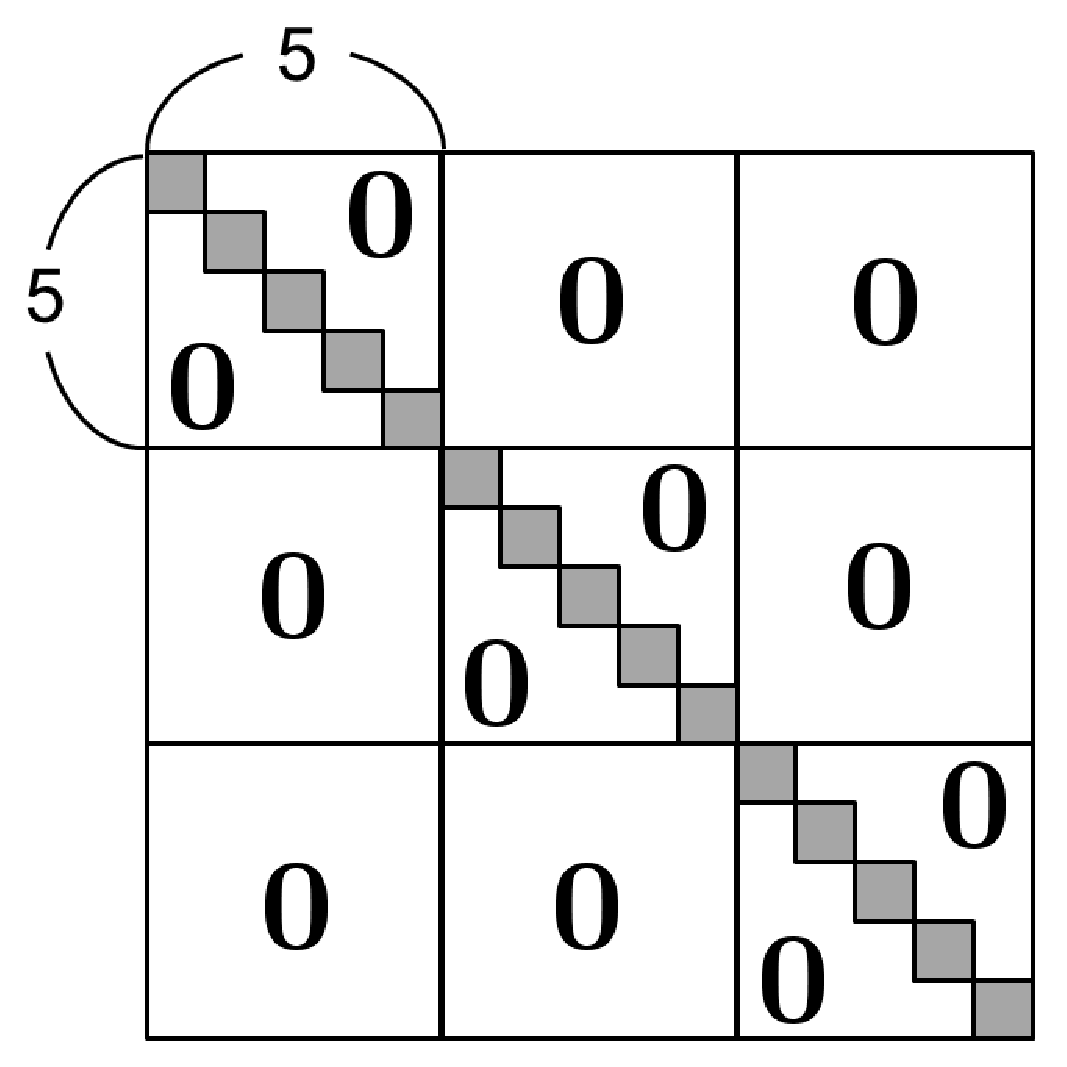
\includegraphics[width=0.8\hsize]{fig/GMM_1.eps}
      \\ (a) diagonal \\(without -c1 and -c2 option)
     \end{center}
    \vspace{3mm}
    \begin{center}
     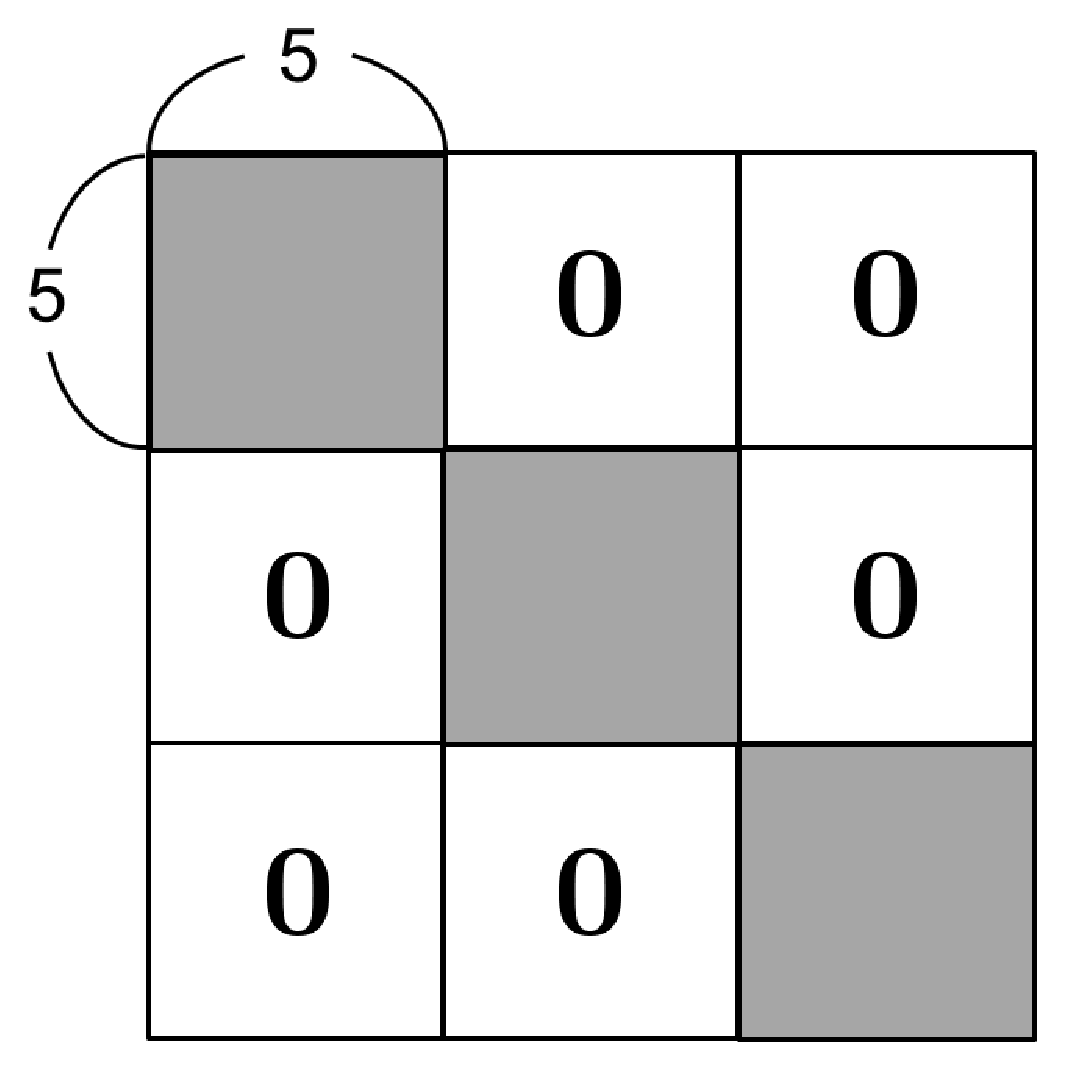
\includegraphics[width=0.8\hsize]{fig/GMM_3.eps}
    \\ (c) block-wise full covariance \\(with -c2 option)
    \end{center}
   \end{minipage}
   \begin{minipage}[b]{0.45\hsize}
    \begin{center}
     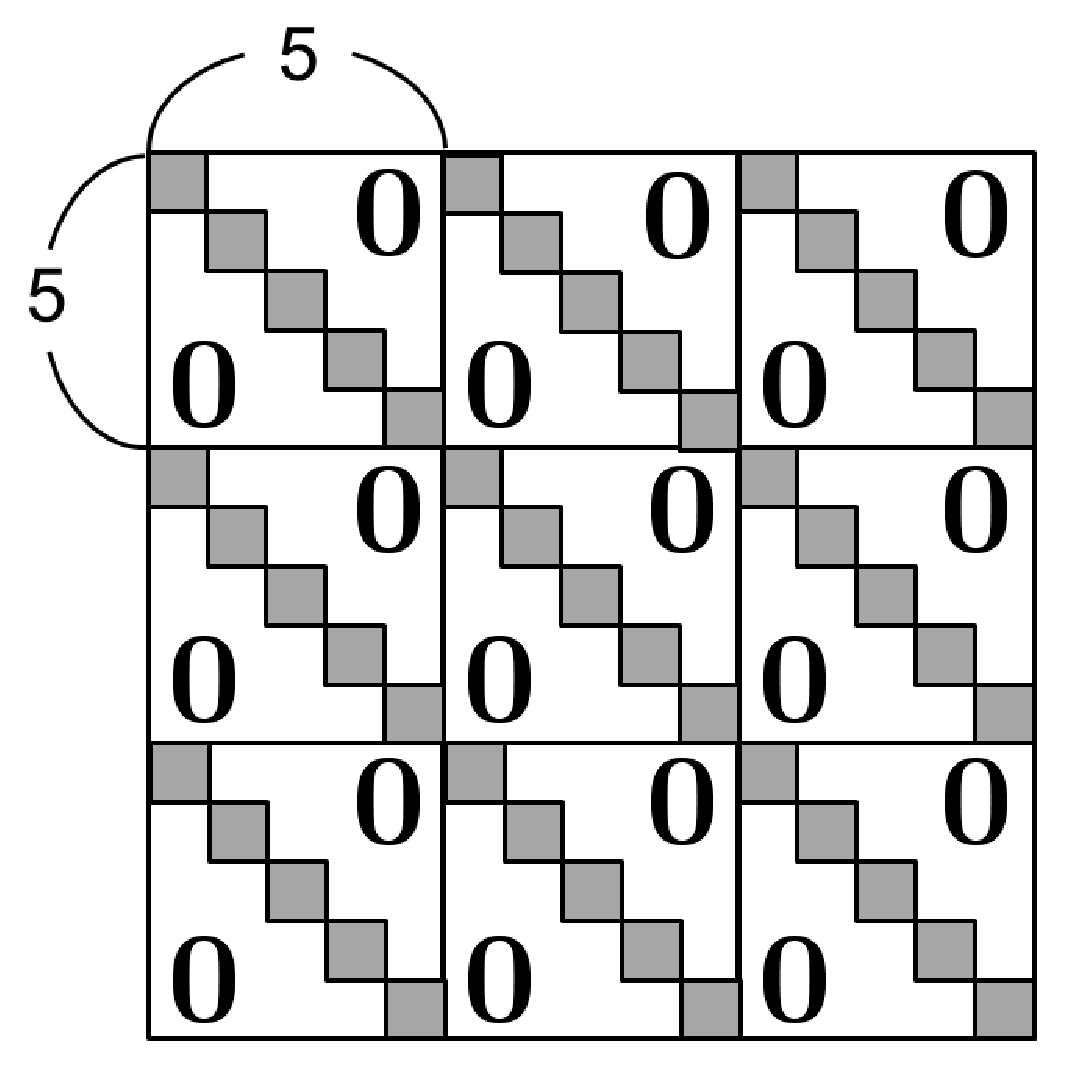
\includegraphics[width=0.8\hsize]{fig/GMM_2.eps}
     \\ (b) inter-block correlation \\(with -c1 option)
    \end{center}
    \vspace{3mm}
    \begin{center}
     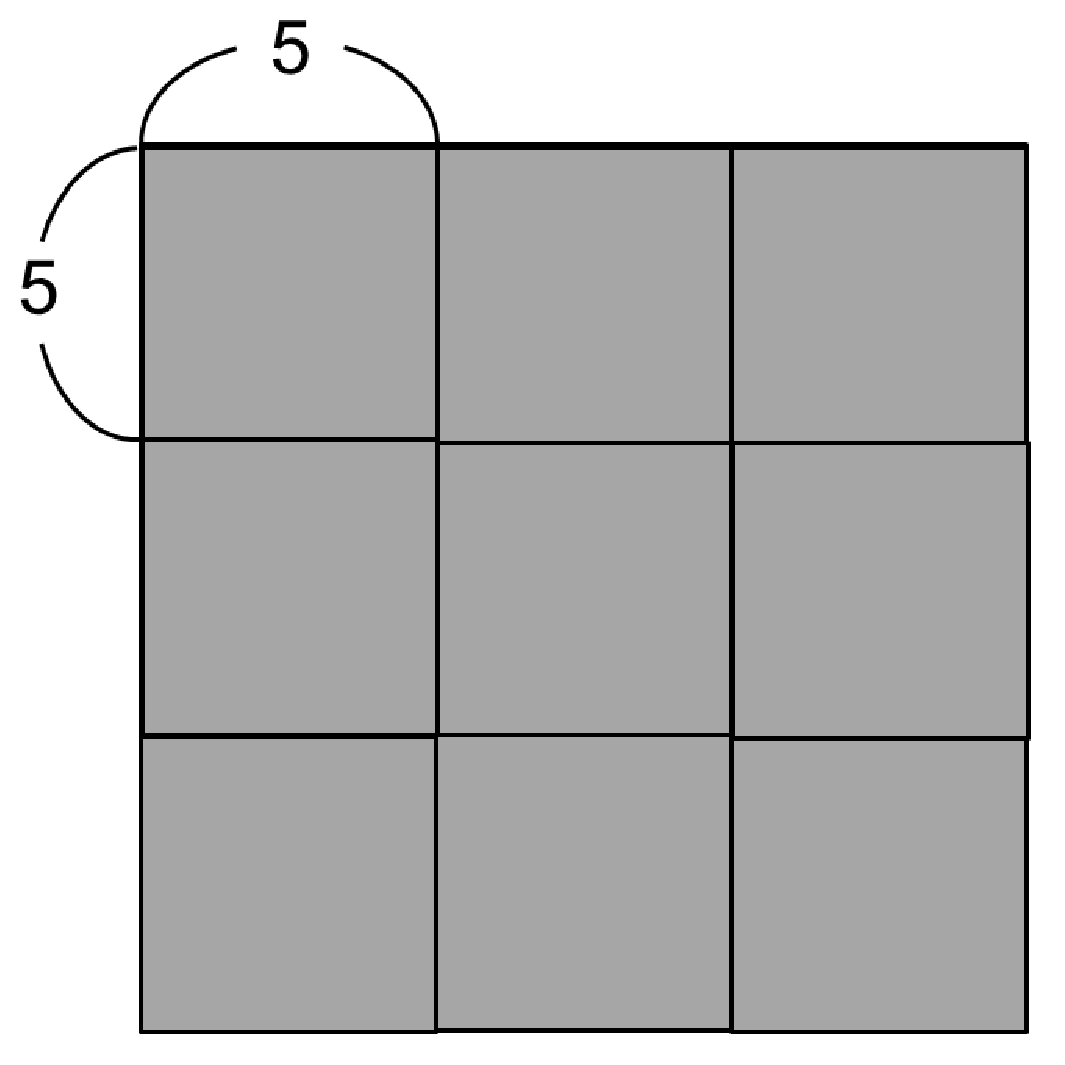
\includegraphics[width=0.8\hsize]{fig/GMM_4.eps}
     \\ (d) full covariance \\(with both -c1 and -c2 option)
    \end{center}
   \end{minipage}
  \end{tabular}
 \end{center}
 \caption{Examples of the structure of covariance matrix}
 \label{fig:gmm_c1}
 \end{figure}
\end{qsection}

\newpage

\begin{qsection}{NOTICE}
\begin{itemize}
\item The -e option specifies a threshold for the change of average
 log-likelihood for training data at each iteration.
\item The -F option specifies a GMM initial parameter file in which
weight, mean, and variance parameters must be aligned in the same
order as output.
\item The -B option specifies the size of each blocks in covariance matrix.
\item The -c1 and -c2 option must be used with -B option. Without -c1 and
-c2 option, a diagonal covariance can be obtained.
\end{itemize}
\end{qsection}

\begin{qsection}{SEE ALSO}
\hyperlink{gmmp}{gmmp},
\hyperlink{lbg}{lbg}
\end{qsection}

% ----------------------------------------------------------------- %
%             The Speech Signal Processing Toolkit (SPTK)           %
%             developed by SPTK Working Group                       %
%             http://sp-tk.sourceforge.net/                         %
% ----------------------------------------------------------------- %
%                                                                   %
%  Copyright (c) 1984-2007  Tokyo Institute of Technology           %
%                           Interdisciplinary Graduate School of    %
%                           Science and Engineering                 %
%                                                                   %
%                1996-2015  Nagoya Institute of Technology          %
%                           Department of Computer Science          %
%                                                                   %
% All rights reserved.                                              %
%                                                                   %
% Redistribution and use in source and binary forms, with or        %
% without modification, are permitted provided that the following   %
% conditions are met:                                               %
%                                                                   %
% - Redistributions of source code must retain the above copyright  %
%   notice, this list of conditions and the following disclaimer.   %
% - Redistributions in binary form must reproduce the above         %
%   copyright notice, this list of conditions and the following     %
%   disclaimer in the documentation and/or other materials provided %
%   with the distribution.                                          %
% - Neither the name of the SPTK working group nor the names of its %
%   contributors may be used to endorse or promote products derived %
%   from this software without specific prior written permission.   %
%                                                                   %
% THIS SOFTWARE IS PROVIDED BY THE COPYRIGHT HOLDERS AND            %
% CONTRIBUTORS "AS IS" AND ANY EXPRESS OR IMPLIED WARRANTIES,       %
% INCLUDING, BUT NOT LIMITED TO, THE IMPLIED WARRANTIES OF          %
% MERCHANTABILITY AND FITNESS FOR A PARTICULAR PURPOSE ARE          %
% DISCLAIMED. IN NO EVENT SHALL THE COPYRIGHT OWNER OR CONTRIBUTORS %
% BE LIABLE FOR ANY DIRECT, INDIRECT, INCIDENTAL, SPECIAL,          %
% EXEMPLARY, OR CONSEQUENTIAL DAMAGES (INCLUDING, BUT NOT LIMITED   %
% TO, PROCUREMENT OF SUBSTITUTE GOODS OR SERVICES; LOSS OF USE,     %
% DATA, OR PROFITS; OR BUSINESS INTERRUPTION) HOWEVER CAUSED AND ON %
% ANY THEORY OF LIABILITY, WHETHER IN CONTRACT, STRICT LIABILITY,   %
% OR TORT (INCLUDING NEGLIGENCE OR OTHERWISE) ARISING IN ANY WAY    %
% OUT OF THE USE OF THIS SOFTWARE, EVEN IF ADVISED OF THE           %
% POSSIBILITY OF SUCH DAMAGE.                                       %
% ----------------------------------------------------------------- %
\hypertarget{gmmp}{}
\name{gmmp}{calculation of GMM log-probability}{probability calculation}

\begin{synopsis}
\item [gmmp] [ --l $L$ ] [ --m $M$ ] [ --a ] [ --f ] [ --B $B1,B2,...$
] [ --c1 ] [ --c2 ] [ --D ] {\em gmmfile} [ {\em infile} ]
\end{synopsis}

\begin{qsection}{DESCRIPTION}
{\em gmmp} calculates GMM log-probabilities of input vectors from {\em
infile} (or standard input). 
The {\em gmmfile} has the same file format as the one generated by the {\em gmm} command,
i.e., {\em gmmfile} consists of $M$ mixture weights
$\bw$ and $M$ Gaussians with mean vector $\bmu$ and diagonal variance vector
$\bv$, each of length $L$:
\begin{align}
 \lambda =
 \left[\bw,\right.&\left.\bmu(0),\bv(0), \bmu(1), \bv(1),
 \ldots, \bmu(M-1), \bv(M-1)\right],\notag\\[2mm]
 \bw &=\left[ w(0), w(1), \ldots, w(M-1) \right],\notag\\
 \bmu(m) &=\left[\mu_m(0), \mu_m(1), \ldots, \mu_m(L-1)\right],\notag\\
 \bv(m) &=\left[\sigma_m^2(0), \sigma_m^2(1), \ldots,
 \sigma_m^2(L-1)\right].\notag
\end{align}


The input sequence consists of $T$ float vectors $\bx$, each of
size $L$:
\begin{displaymath}
 \bx(0), \bx(1), \dots, \bx(T-1).
\end{displaymath}
The result is a sequence of log-probabilities of input vectors:
\begin{displaymath}
 \log b(\bx(0)), \log b(\bx(1)), \ldots, \log b(\bx(T-1)),
\end{displaymath}
or an average log-probability (if -a option is used):
\begin{displaymath}
 \log P(\bX) = \frac{1}{T}\sum_{t=0}^{T-1}\log b(\bx(t)),
\end{displaymath}
where
\begin{align}
 &b(\bx(t)) =\sum_{m=0}^{M-1}
 w(m){\cal N}(\bx(t) \; ; \; \bmu(m),\bv(m)),\notag\\
 &{\cal N}(\bx(t) \; ; \; \bmu(m),\bv(m))%
  =\frac{1}{(2\pi)^{L/2}\prod_{l=0}^{L-1}\sigma_m(l)}%
  \exp{\left\{-\frac{1}{2}%
    \sum_{l=0}^{L-1}
    \frac{\left(x_t(l)-\mu_m(l)\right)^2}%
    {\sigma_m^2(l)}\right\}}.\notag
\end{align}

\end{qsection}

\begin{options}
 \argm{l}{L}{length of vector}{26}
 \argm{m}{M}{number of Gaussian components}{16}
 \argm{f}{}{full covariance}{FALSE}
 \argm{a}{}{print average log-probability}{FALSE}
 \desc[1ex]{(level 2)}
 \argm{B}{B1~B2~$\ldots$~Bn}{block size in covariance matrix,\\
                             where $(B1+B2+\ldots+Bn)=L$}{FALSE}
 \argm{c1}{}{inter-block correlation}{FALSE}
 \argm{c2}{}{full covariance in each block}{FALSE}
 \argm{D}{}{print log-probability of each block}{FALSE}
\end{options}

\begin{qsection}{EXAMPLE}
In the following example, frame log-probabilities of input data {\em
data.f} for GMM with 8 Gaussians {\em gmm.f} are written to {\em
probs.f}.

\begin{quote}
\verb! gmmp -m 8 gmm.f data.f > probs.f!
\end{quote}
\end{qsection}

\begin{qsection}{SEE ALSO}
\hyperlink{gmm}{gmm}
\end{qsection}

% ----------------------------------------------------------------
%       Speech Signal Processing Toolkit (SPTK): version 3.0
%                      SPTK Working Group
% 
%                Department of Computer Science
%                Nagoya Institute of Technology
%                             and
%   Interdisciplinary Graduate School of Science and Engineering
%                Tokyo Institute of Technology
%                   Copyright (c) 1984-2000
%                     All Rights Reserved.
% 
% Permission is hereby granted, free of charge, to use and
% distribute this software and its documentation without
% restriction, including without limitation the rights to use,
% copy, modify, merge, publish, distribute, sublicense, and/or
% sell copies of this work, and to permit persons to whom this
% work is furnished to do so, subject to the following conditions:
% 
%   1. The code must retain the above copyright notice, this list
%      of conditions and the following disclaimer.
% 
%   2. Any modifications must be clearly marked as such.
%                                                                        
% NAGOYA INSTITUTE OF TECHNOLOGY, TOKYO INSITITUTE OF TECHNOLOGY,
% SPTK WORKING GROUP, AND THE CONTRIBUTORS TO THIS WORK DISCLAIM
% ALL WARRANTIES WITH REGARD TO THIS SOFTWARE, INCLUDING ALL
% IMPLIED WARRANTIES OF MERCHANTABILITY AND FITNESS, IN NO EVENT
% SHALL NAGOYA INSTITUTE OF TECHNOLOGY, TOKYO INSITITUTE OF
% TECHNOLOGY, SPTK WORKING GROUP, NOR THE CONTRIBUTORS BE LIABLE
% FOR ANY SPECIAL, INDIRECT OR CONSEQUENTIAL DAMAGES OR ANY
% DAMAGES WHATSOEVER RESULTING FROM LOSS OF USE, DATA OR PROFITS,
% WHETHER IN AN ACTION OF CONTRACT, NEGLIGENCE OR OTHER TORTIOUS
% ACTION, ARISING OUT OF OR IN CONNECTION WITH THE USE OR
% PERFORMANCE OF THIS SOFTWARE.
% ----------------------------------------------------------------
%
\name{gnorm}{gain normalization}{speech parameter transformation}

\begin{synopsis}
\item [gnorm] [ --m $M$ ] [ --g $G$ ] [ {\em infile} ]
\end{synopsis}

\begin{qsection}{DESCRIPTION}
{\em gnorm} normalizes generalized cepstrum coefficients $c_\gamma(m)$ 
from {\em infile} (or standard input), 
sending the normalized generalized cepstrum coefficients to standard output.

Input and output data are in float format.

The normalized generalized cepstrum coefficients $c_\gamma'(m)$
can be written as
\begin{displaymath}
c_\gamma'(m) = \frac{c_\gamma(m)}{1+\gamma c_\gamma(0)}, ~~~m>0
\end{displaymath}
Also, the gain $K = c_\gamma'(0)$ is
\begin{displaymath}
K = \left\{
	\begin{array}{ll} \displaystyle
	  \left(\frac{1}{1+\gamma c_\gamma(0)}\right)^{1/\gamma},
		& 0<|\gamma|\leq 1 \\ \displaystyle
	  \exp c_\gamma(0),  & \gamma=0
	\end{array} \right.
\end{displaymath}
\end{qsection}

\begin{options}
	\argm{m}{M}{order of generalized cepstrum}{25}
	\argm{g}{G}{power parameter $\gamma$ of generalized cepstrum,\\
		    if $G>1.0$ then $\gamma=-1/G$}{0}
\end{options}

\begin{qsection}{EXAMPLE}
In this example, generalized cepstrum coefficients in float format
are read from file {\em data.gcep} )$(M=15, \gamma=-0.5)$,
normalized and outputed to {\em data.ngcep}:
\begin{quote}
 \verb!gnorm -m 15 -g 2 < data.gcep > data.ngcep!
\end{quote} 
\end{qsection}

\begin{qsection}{SEE ALSO}
 ignorm, gcep, mgcep, gc2gc, mgc2mgc, freqt
\end{qsection}

% ----------------------------------------------------------------
%       Speech Signal Processing Toolkit (SPTK): version 3.0
%                      SPTK Working Group
% 
%                Department of Computer Science
%                Nagoya Institute of Technology
%                             and
%   Interdisciplinary Graduate School of Science and Engineering
%                Tokyo Institute of Technology
%                   Copyright (c) 1984-2000
%                     All Rights Reserved.
% 
% Permission is hereby granted, free of charge, to use and
% distribute this software and its documentation without
% restriction, including without limitation the rights to use,
% copy, modify, merge, publish, distribute, sublicense, and/or
% sell copies of this work, and to permit persons to whom this
% work is furnished to do so, subject to the following conditions:
% 
%   1. The code must retain the above copyright notice, this list
%      of conditions and the following disclaimer.
% 
%   2. Any modifications must be clearly marked as such.
%                                                                        
% NAGOYA INSTITUTE OF TECHNOLOGY, TOKYO INSITITUTE OF TECHNOLOGY,
% SPTK WORKING GROUP, AND THE CONTRIBUTORS TO THIS WORK DISCLAIM
% ALL WARRANTIES WITH REGARD TO THIS SOFTWARE, INCLUDING ALL
% IMPLIED WARRANTIES OF MERCHANTABILITY AND FITNESS, IN NO EVENT
% SHALL NAGOYA INSTITUTE OF TECHNOLOGY, TOKYO INSITITUTE OF
% TECHNOLOGY, SPTK WORKING GROUP, NOR THE CONTRIBUTORS BE LIABLE
% FOR ANY SPECIAL, INDIRECT OR CONSEQUENTIAL DAMAGES OR ANY
% DAMAGES WHATSOEVER RESULTING FROM LOSS OF USE, DATA OR PROFITS,
% WHETHER IN AN ACTION OF CONTRACT, NEGLIGENCE OR OTHER TORTIOUS
% ACTION, ARISING OUT OF OR IN CONNECTION WITH THE USE OR
% PERFORMANCE OF THIS SOFTWARE.
% ----------------------------------------------------------------
%
\name{grlogsp}{$B%i%s%K%s%0BP?t%9%Z%/%H%k$N%W%m%C%H(B}{$B%0%i%UI=<((B}

\begin{synopsis}
\item[grlogsp] [ --t ] [ --O $O$ ] [ --x $X$ ] [ --y $ymin$ ] [ --yy $YY$ ]
	       [ --yo $YO$ ] [ --p $P$ ] 
\item[\ ~~~~~~~~] [ --ln $LN$ ] [ --s $S$ ] [ --e $E$ ] [ --n $N$ ] [ --l $L$ ] 
\item[\ ~~~~~~~~] [ --c $comment1$ ] [ --c2 $comment2$ ] [ --c3 $comment3$ ]
		  [ {\em infile} ]
\end{synopsis}

\begin{qsection}{DESCRIPTION}
{\em grlogsp}$B$O!"(Bfloat$B7?$N%G!<%?$rI8=`F~NO$+$iFI$_9~$s$G!$$=$N%i%s%K%s%0(B
$B%9%Z%/%H%k$r%0%i%UI=<($9$k%W%m%C%?$N%3%^%s%INs$r@8@.$7$^$9!%(B
$B=>$C$F!$(B{\em xgr}$B%3%^%s%IEy$HJ;MQ$7$F;H$$$^$9!%(B
$B<BBN$O%7%'%k%9%/%j%W%H$G!$FbIt$G$O(B{\em fig}$B$H(B{\em fdrw}$B$rMQ$$$F$$$^$9!%(B
\end{qsection}

\begin{options}
	\argm{t}{}{x$B<4$H(By$B<4$rF~$l49$($k(B}{FALSE}
	\argm{O}{O}{$B%0%i%U$N3+;OE@!%(B\\
		      \begin{minipage}{4cm}
		      \begin{tabular}{ccc}
			1 & ( 25,$YO$) & [mm] \\
			2 & ( 60,$YO$) & [mm] \\
			3 & ( 95,$YO$) & [mm] \\
			4 & (130,$YO$) & [mm] \\
			5 & (165,$YO$) & [mm]
		      \end{tabular}\\\hspace*{\fill}
		      \end{minipage}
		      \begin{minipage}{4cm}
			    \epsffile{fig/grlogsp-on.eps}
		      \end{minipage}\\\hspace*{\fill}\\
		    -t $B%*%W%7%g%s$,;XDj$5$l$F$$$k>l9g$O!"(B
		    $(YO + 100 , X)$ [mm]$B$N0LCV$K%0%i%U$r=q$-$^$9!%(B}{1}
	\argm{x}{X}{ $x$ $B<4$N%9%1!<%k!%(B\\
		       \begin{tabular}{cl}
			1 & $B@55,2=$5$l$?<~GH?t(B($0 \sim 0.5$) \\
			2 & $B@55,2=$5$l$?<~GH?t(B($0 \sim \pi$) \\
			4 & $B<~GH?t(B($0 \sim 4$kHz) \\
			5 & $B<~GH?t(B($0 \sim 5$kHz) \\
			8 & $B<~GH?t(B($0 \sim 8$kHz) \\
			10 & $B<~GH?t(B($0 \sim 10$kHz) \\
		       \end{tabular}\\\hspace*{\fill}}{1}
	\argm{y}{ymin}{ $y$ $B<4$N%9%1!<%j%s%0$N:G>.CM!%(B}{-100}
	\argm{yy}{YY}{ $y$ $B<4$N%9%1!<%j%s%0(B[dB/10mm]$B$NHO0O!%(B}{100}
	\argm{yo}{YO}{ $y$ $B<4$N%*%U%;%C%H!%(B}{30}
	\argm{p}{p}{$B;HMQ$9$k%Z%sHV9f(B($1 \sim 10$)$B!%(B}{2}
	\argm{ln}{LN}{$BIA2h$9$k:]$N@~$N<oN`(B($0 \sim 5$)$B!%!c(Bfig$B;2>H!d!%(B}{1}
	\argm{s}{S}{$BF~NO$9$k%G!<%?$N2?%U%l!<%`L\$+$i%0%i%U$K=q$/$+$r;XDj!%(B}{0}
	\argm{e}{E}{$BF~NO$9$k%G!<%?$N2?%U%l!<%`L\$^$G%0%i%U$K=q$/$+$r;XDj!%(B}{EOF}
	\argm{n}{N}{$B%i%s%K%s%0%W%m%C%H$9$k%G!<%?$N%U%l!<%`?t!%(B}{EOF}
	\argm{l}{L}{$B%U%l!<%`D9!%(B $B<B:]$K$O(B $\frac{L}{2}$ $B8D$N%G!<%?$r(B
		      $B%0%i%U$K=q$/!%(B}{256}
	\argm{c, c2, c3}{\mbox{\em comment} 1 \sim 3}{$B%0%i%U$N%3%a%s%H!%(B}{N/A}
	\desc[1zh]{$BDL>o(B,$B0J2<$N%*%W%7%g%s$N;XDj$NI,MW$O$"$j$^$;$s!%(B}
	\argm{W}{W}{$B%0%i%U$NI}(B($\times 100$mm)$B!%(B}{0.25}
	\argm{H}{H}{$B%0%i%U$N9b$5(B($\times 100$mm)$B!%(B}{1.5}
	\argm{z}{Z}{$B%i%s%K%s%0%9%Z%/%H%k$rIA2h$9$k:]!"3F%U%l!<%`$r(B $y$ $B<4J}8~(B
		    $B$K$:$i$95wN%(B(mm)$B!%(B}{1}
	\argm{o}{xo \; yo}{$B%0%i%U$N3+;OE@$r(Bmm $BC10L$G;XDj!%(B --o $B%*%W%7%g%s$,(B
			   $B;XDj$5$l$k$H(B --O $B%*%W%7%g%s$OL58z!%(B}{95 30}
	\argm{g}{G}{$B%0%i%U$NOH$N7A<0(B($0 \sim 2$)$B!%!c(Bfig$B;2>H!d!%(B}{2}
	\argm{cy}{cy}{1$BHVL\$N%3%a%s%H$N0LCV!%(B}{-8}
	\argm{cy2}{cy2}{2$BHVL\$N%3%a%s%H$N0LCV!%(B}{-14}
	\argm{cy3}{cy3}{3$BHVL\$N%3%a%s%H$N0LCV!%(B}{-20}
	\argm{cs}{cs}{$B%3%a%s%H$N%5%$%:!%(B}{1}
	\argm{f}{f}{fig$B%3%^%s%IMQ$NDI2C%G!<%?%U%!%$%k!%(B}{NULL}
\end{options}

\begin{qsection}{EXAMPLE}
float$B7A<0$N%U%!%$%k(B {\em data.f} $B$N%G!<%?$NBP?t?6I}%9%Z%/%H%k$r5a$a!$(B
$B%i%s%K%s%0%W%m%C%H$7$?%0%i%U$r(BPostScript$B7A<0$G(Bdata.ps$B$K=q$-9~$`(B:
\begin{quote}
 \verb!frame < data.f | window |\! \\
 \verb!uels -m 15 | c2sp -m 15 |\! \\
 \verb!grlogsp | psgr > data.ps!
 \end{quote}
\end{qsection}

\begin{qsection}{SEE ALSO}
 fig, fdrw, xgr, psgr, glogsp, gwave
\end{qsection}

% ----------------------------------------------------------------- %
%             The Speech Signal Processing Toolkit (SPTK)           %
%             developed by SPTK Working Group                       %
%             http://sp-tk.sourceforge.net/                         %
% ----------------------------------------------------------------- %
%                                                                   %
%  Copyright (c) 1984-2007  Tokyo Institute of Technology           %
%                           Interdisciplinary Graduate School of    %
%                           Science and Engineering                 %
%                                                                   %
%                1996-2014  Nagoya Institute of Technology          %
%                           Department of Computer Science          %
%                                                                   %
% All rights reserved.                                              %
%                                                                   %
% Redistribution and use in source and binary forms, with or        %
% without modification, are permitted provided that the following   %
% conditions are met:                                               %
%                                                                   %
% - Redistributions of source code must retain the above copyright  %
%   notice, this list of conditions and the following disclaimer.   %
% - Redistributions in binary form must reproduce the above         %
%   copyright notice, this list of conditions and the following     %
%   disclaimer in the documentation and/or other materials provided %
%   with the distribution.                                          %
% - Neither the name of the SPTK working group nor the names of its %
%   contributors may be used to endorse or promote products derived %
%   from this software without specific prior written permission.   %
%                                                                   %
% THIS SOFTWARE IS PROVIDED BY THE COPYRIGHT HOLDERS AND            %
% CONTRIBUTORS "AS IS" AND ANY EXPRESS OR IMPLIED WARRANTIES,       %
% INCLUDING, BUT NOT LIMITED TO, THE IMPLIED WARRANTIES OF          %
% MERCHANTABILITY AND FITNESS FOR A PARTICULAR PURPOSE ARE          %
% DISCLAIMED. IN NO EVENT SHALL THE COPYRIGHT OWNER OR CONTRIBUTORS %
% BE LIABLE FOR ANY DIRECT, INDIRECT, INCIDENTAL, SPECIAL,          %
% EXEMPLARY, OR CONSEQUENTIAL DAMAGES (INCLUDING, BUT NOT LIMITED   %
% TO, PROCUREMENT OF SUBSTITUTE GOODS OR SERVICES; LOSS OF USE,     %
% DATA, OR PROFITS; OR BUSINESS INTERRUPTION) HOWEVER CAUSED AND ON %
% ANY THEORY OF LIABILITY, WHETHER IN CONTRACT, STRICT LIABILITY,   %
% OR TORT (INCLUDING NEGLIGENCE OR OTHERWISE) ARISING IN ANY WAY    %
% OUT OF THE USE OF THIS SOFTWARE, EVEN IF ADVISED OF THE           %
% POSSIBILITY OF SUCH DAMAGE.                                       %
% ----------------------------------------------------------------- %
\hypertarget{grpdelay}{}
\name{grpdelay}{group delay of digital filter}{signal processing}
\begin{synopsis}
 \item[grpdelay] [ --l $L$ ] [ --m $M$ ] [ --a ] [ {\em infile} ] 
\end{synopsis}

\begin{qsection}{DESCRIPTION}
{\em grpdelay} computes the group delay of a sequence of filter coefficients 
from {\em infile} (or standard input), 
sending the result to standard output.
Input and output data are in float format.
\par
If the {\bf --m} option is omitted
and the length of an input data sequence is less than FFT size,
the input file is padded with 0's and the FFT is evaluated
as exemplified below.
When the {\bf --a} option is given,
the gain is obtained from zero order input.
\par
\[
\begin{array}{lll}
\mbox{Input sequence} & 
\overbrace{\framebox[4.5cm]{$x_0, x_1, \ldots, x_{M}, 0,
					\ldots,0$}}^{L}  & \mbox{filter coefficients}\\
		& \makebox[4.5cm]{0\hfill $L-1$} &
\end{array}
\]
\[
\begin{array}{lll}
\mbox{Output sequence} & \overbrace{\framebox[4.5cm]{$\tau(\omega)$}}^{L/2+1} &
	   \mbox{group delay}\\
		& \makebox[4.5cm]{0\hfill $L-1$} &

\end{array}
\]
\end{qsection}

\begin{options}
	\argm{l}{L}{FFT size power of 2}{256}
	\argm{m}{M}{order of filter}{L-1}
	\argm{a}{}{ARMA filter}{FALSE}
\end{options}


\begin{qsection}{EXAMPLE}
This example plots in the screen the group delay of impulse response
of the filter with the following transfer function.
\begin{displaymath}
  H(z)=\frac{1}{1+0.9z^{-1}}
\end{displaymath}
\begin{quote}
\verb! impulse | dfs -a 1 0.9 | grpdelay | fdrw | xgr !
\end{quote}  
\end{qsection}

\begin{qsection}{SEE ALSO}
\hyperlink{delay}{delay},
\hyperlink{phase}{phase}
\end{qsection}

% ----------------------------------------------------------------- %
%             The Speech Signal Processing Toolkit (SPTK)           %
%             developed by SPTK Working Group                       %
%             http://sp-tk.sourceforge.net/                         %
% ----------------------------------------------------------------- %
%                                                                   %
%  Copyright (c) 1984-2007  Tokyo Institute of Technology           %
%                           Interdisciplinary Graduate School of    %
%                           Science and Engineering                 %
%                                                                   %
%                1996-2016  Nagoya Institute of Technology          %
%                           Department of Computer Science          %
%                                                                   %
% All rights reserved.                                              %
%                                                                   %
% Redistribution and use in source and binary forms, with or        %
% without modification, are permitted provided that the following   %
% conditions are met:                                               %
%                                                                   %
% - Redistributions of source code must retain the above copyright  %
%   notice, this list of conditions and the following disclaimer.   %
% - Redistributions in binary form must reproduce the above         %
%   copyright notice, this list of conditions and the following     %
%   disclaimer in the documentation and/or other materials provided %
%   with the distribution.                                          %
% - Neither the name of the SPTK working group nor the names of its %
%   contributors may be used to endorse or promote products derived %
%   from this software without specific prior written permission.   %
%                                                                   %
% THIS SOFTWARE IS PROVIDED BY THE COPYRIGHT HOLDERS AND            %
% CONTRIBUTORS "AS IS" AND ANY EXPRESS OR IMPLIED WARRANTIES,       %
% INCLUDING, BUT NOT LIMITED TO, THE IMPLIED WARRANTIES OF          %
% MERCHANTABILITY AND FITNESS FOR A PARTICULAR PURPOSE ARE          %
% DISCLAIMED. IN NO EVENT SHALL THE COPYRIGHT OWNER OR CONTRIBUTORS %
% BE LIABLE FOR ANY DIRECT, INDIRECT, INCIDENTAL, SPECIAL,          %
% EXEMPLARY, OR CONSEQUENTIAL DAMAGES (INCLUDING, BUT NOT LIMITED   %
% TO, PROCUREMENT OF SUBSTITUTE GOODS OR SERVICES; LOSS OF USE,     %
% DATA, OR PROFITS; OR BUSINESS INTERRUPTION) HOWEVER CAUSED AND ON %
% ANY THEORY OF LIABILITY, WHETHER IN CONTRACT, STRICT LIABILITY,   %
% OR TORT (INCLUDING NEGLIGENCE OR OTHERWISE) ARISING IN ANY WAY    %
% OUT OF THE USE OF THIS SOFTWARE, EVEN IF ADVISED OF THE           %
% POSSIBILITY OF SUCH DAMAGE.                                       %
% ----------------------------------------------------------------- %
\hypertarget{gseries}{}
\name{gseries}{draw a discrete series}{plotting graphs}

\begin{synopsis}
\item[gseries] [ --F $F$] [ --s $S$ ] [ --e $E$ ] [ --n $N$ ] [ --i $I$ ] [ --y $ymax$ ]
               [ --y2 $ymin$ ] [--m $M$ ] 
\item[\ ~~~~~~~~] [ --p $P$ ] [ --magic $magic$ ] [ --MAGIC $MAGIC$ ] [ +{\em type} ]  [ {\em infile} ]

\end{synopsis}

\begin{qsection}{DESCRIPTION}
{\em gseries} converts discrete series data
from {\em infile} (or standard input) to FP5301 plot format, 
sending the result to standard output. 
The output can viewed with \hyperlink{xgr}{xgr}.

{\em gseries} is implemented as a shell script 
that uses the \hyperlink{fig}{fig} command.
\end{qsection}

\begin{options}
        \argm{F}{F}{factor}{1}
        \argm{s}{S}{start point}{0}
        \argm{e}{E}{end point}{EOF}
        \argm{n}{N}{data number of one screen\\
                    if this option is omitted,
                    all of the data is plotted on one screen.}{N/A}
        \argm{i}{I}{number of screen}{5}
        \argm{y}{ymax}{maximum amplitude\\
                       if this option is omitted,
                       ymax is maximum value of the input data.}{N/A}
        \argm{y2}{ymin}{minimum amplitude}{-YMAX}
        \argm{m}{M}{mark type}{1}
        \argm{p}{P}{pen type($1 \sim 10$)}{1}
        \argm{magic}{magic}{remove magic number}{FALSE}
        \argm{MAGIC}{MAGIC}{replace magic number by $MAGIC$ \\
                            if -magic option is not given, return error.\\
                        if -magic or -MAGIC option is given multiple
                        times, also return error.}{FALSE}
        \argp{t}{Input data format\\ 
                \begin{tabular}{llcll} \\[-1ex]
                        c & char (1 byte) & \quad &
                        C & unsigned char (1 byte) \\
                        s & short (2 bytes) & \quad &
                        S & unsigned short (2 bytes) \\
                        i3 & int (3 bytes) & \quad &
                        I3 & unsigned int (3 bytes) \\
                        i & int (4 bytes) & \quad &
                        I & unsigned int (4 bytes) \\
                        l & long (4 bytes) & \quad &
                        L & unsigned long (4 bytes) \\
                        le & long long (8 bytes) & \quad &
                        LE & unsigned long long (8 bytes) \\
                        f & float (4 bytes) & \quad &
                        d & double (8 bytes) \\
                        de & long double (12 bytes) & \quad &
                \end{tabular}}{f}
\end{options}

\begin{qsection}{EXAMPLE}
 In the following example, {\em gseries} reads impulse response
 in float format from {\em data.f} and writes the output
 in encapsulated Postscript format to {\em data.eps}.
 \begin{quote}
 \verb!gseries +f < data.f | psgr > data.eps!
 \end{quote}
The following example replaces the magic number 0 in {\em data.f} by 1.0 and
writes the output to {\em data.eps}.
\begin{quote}
  \verb!gseriese +f -magic 0 -MAGIC 1.0 < data.f | \!\\
  \verb!psgr > data.eps!
\end{quote}
Also, the following example removes the magic number 0 in {\em data.f}.
\begin{quote}
  \verb!gseriese +f -magic 0 < data.f | psgr > data.eps!
\end{quote}
\end{qsection}

\begin{qsection}{NOTICE}
\begin{itemize}
\item If options of amplitude are not used, value of amplitude is
automatically determined.
\item If --n option is not used, entire impluse response is displayed.
\item Can not use --n option and --i option. 
\item If --magic option is not given, return error. 
\item If --magic or --MAGIC option is given mutiple times, return
error.
\end{itemize}
\end{qsection}

\begin{qsection}{SEE ALSO}
\hyperlink{fig}{fig},
\hyperlink{fdrw}{fdrw},
\hyperlink{xgr}{xgr},
\hyperlink{psgr}{psgr},
\hyperlink{glogsp}{glogsp},
\hyperlink{grlogsp}{grlogsp},
\hyperlink{gwave}{gwave}
\end{qsection}

% ----------------------------------------------------------------- %
%             The Speech Signal Processing Toolkit (SPTK)           %
%             developed by SPTK Working Group                       %
%             http://sp-tk.sourceforge.net/                         %
% ----------------------------------------------------------------- %
%                                                                   %
%  Copyright (c) 1984-2007  Tokyo Institute of Technology           %
%                           Interdisciplinary Graduate School of    %
%                           Science and Engineering                 %
%                                                                   %
%                1996-2009  Nagoya Institute of Technology          %
%                           Department of Computer Science          %
%                                                                   %
% All rights reserved.                                              %
%                                                                   %
% Redistribution and use in source and binary forms, with or        %
% without modification, are permitted provided that the following   %
% conditions are met:                                               %
%                                                                   %
% - Redistributions of source code must retain the above copyright  %
%   notice, this list of conditions and the following disclaimer.   %
% - Redistributions in binary form must reproduce the above         %
%   copyright notice, this list of conditions and the following     %
%   disclaimer in the documentation and/or other materials provided %
%   with the distribution.                                          %
% - Neither the name of the SPTK working group nor the names of its %
%   contributors may be used to endorse or promote products derived %
%   from this software without specific prior written permission.   %
%                                                                   %
% THIS SOFTWARE IS PROVIDED BY THE COPYRIGHT HOLDERS AND            %
% CONTRIBUTORS "AS IS" AND ANY EXPRESS OR IMPLIED WARRANTIES,       %
% INCLUDING, BUT NOT LIMITED TO, THE IMPLIED WARRANTIES OF          %
% MERCHANTABILITY AND FITNESS FOR A PARTICULAR PURPOSE ARE          %
% DISCLAIMED. IN NO EVENT SHALL THE COPYRIGHT OWNER OR CONTRIBUTORS %
% BE LIABLE FOR ANY DIRECT, INDIRECT, INCIDENTAL, SPECIAL,          %
% EXEMPLARY, OR CONSEQUENTIAL DAMAGES (INCLUDING, BUT NOT LIMITED   %
% TO, PROCUREMENT OF SUBSTITUTE GOODS OR SERVICES; LOSS OF USE,     %
% DATA, OR PROFITS; OR BUSINESS INTERRUPTION) HOWEVER CAUSED AND ON %
% ANY THEORY OF LIABILITY, WHETHER IN CONTRACT, STRICT LIABILITY,   %
% OR TORT (INCLUDING NEGLIGENCE OR OTHERWISE) ARISING IN ANY WAY    %
% OUT OF THE USE OF THIS SOFTWARE, EVEN IF ADVISED OF THE           %
% POSSIBILITY OF SUCH DAMAGE.                                       %
% ----------------------------------------------------------------- %
\hypertarget{gwave}{}
\name{gwave}{draw a waveform}{plotting graphs}

\begin{synopsis}
\item[gwave] [ --s $S$ ] [ --e $E$ ] [ --n $N$ ] [ --i $I$ ] [ --y $ymax$ ]
               [ --y2 $ymin$ ] [ --p $P$ ] 
\item[\ ~~~~~~~~] [ +{\em type} ]  [ {\em infile} ]

\end{synopsis}

\begin{qsection}{DESCRIPTION}
{\em gwave} converts speech waveform data 
from {\em infile} (or standard input) to FP5301 plot format, 
sending the result to standard output. 
The output can viewed with \hyperlink{xgr}{xgr}.

{\em gwave} is implemented as a shell script 
that uses the \hyperlink{fig}{fig} and \hyperlink{fdrw}{fdrw} commands.
\end{qsection}

\begin{options}
        \argm{s}{S}{start point}{0}
        \argm{e}{E}{end point}{EOF}
        \argm{n}{N}{data number of one screen\\
                    if this option is omitted,
                    all of the data is plotted on one screen.}{N/A}
        \argm{i}{I}{number of screen}{5}
        \argm{y}{ymax}{maximum amplitude\\
                       if this option is omitted,
                       ymax is maximum value of the input data.}{N/A}
        \argm{y2}{ymin}{minimum amplitude}{-YMAX}
        \argm{p}{P}{pen type($1 \sim 10$)}{1}
        \argp{t}{Input data format\\ 
                \begin{tabular}{llcll} \\[-1ex]
                        s & short (2 bytes) & \quad &
                        i & int (4 bytes) \\
                        f & float (4 bytes) & \quad &
                        d & double (8 bytes) \\
                \end{tabular}}{f}
\end{options}

\begin{qsection}{EXAMPLE}
This example reads speech waveform file in float format from
{\em data.f} and writes the output in Postscript format to
{\em data.ps}.
\begin{quote}
 \verb!gwave +f < data.f | psgr > data.ps!
 \end{quote}
\end{qsection}

\begin{qsection}{SEE ALSO}
\hyperlink{fig}{fig},
\hyperlink{fdrw}{fdrw},
\hyperlink{xgr}{xgr},
\hyperlink{psgr}{psgr},
\hyperlink{glogsp}{glogsp},
\hyperlink{grlogsp}{grlogsp}
\end{qsection}

\name{histogram}{histogram}{data processing}

\begin{synopsis}
\item [histogram] [ --l $L$ ] [ --i $I$ ] [ --j $J$ ] [ --s $S$ ] [ --n ] 
                  [ {\em infile} ] 
\end{synopsis}

\begin{qsection}{DESCRIPTION}
This command evaluates the histogram from the assigned file
and sends the results to the standard output.
\par
Input and output data are in float format.
If a graph is wanted, please send the output of ``histogram'' to ``fdrw''.
\par
In case a data value is outside of the assigned interval,
the histogram will evaluate its output but the return value of
the command will be different from $0$.
\end{qsection}

\begin{options}
        \argm{l}{L}{frame size\\
          \begin{tabular}{ll}\\ [-1zh]
            $L>0$ & evaluate the histogram for every frame\\
            $L=0$ & evaluate the histogram for the whole file\\
          \end{tabular}\\\hspace*{\fill}}{0}
        \argm{i}{I}{infimum}{0.0}
        \argm{j}{J}{supremum}{1.0}
        \argm{s}{S}{step size}{0.1}
        \argm{n}{}{normalization}{FALSE}
\end{options}

\begin{qsection}{EXAMPLE}
The example below plots the histogram of the speech waveform file
{\em data.f} in float format.
\begin{quote}
 \verb!histogram -i -16000 -j 16000 -s 100 data.f | fdrw | xgr!
\end{quote} 
\end{qsection}

\begin{qsection}{SEE ALSO}
 average
\end{qsection}

% ----------------------------------------------------------------- %
%             The Speech Signal Processing Toolkit (SPTK)           %
%             developed by SPTK Working Group                       %
%             http://sp-tk.sourceforge.net/                         %
% ----------------------------------------------------------------- %
%                                                                   %
%  Copyright (c) 1984-2007  Tokyo Institute of Technology           %
%                           Interdisciplinary Graduate School of    %
%                           Science and Engineering                 %
%                                                                   %
%                1996-2017  Nagoya Institute of Technology          %
%                           Department of Computer Science          %
%                                                                   %
% All rights reserved.                                              %
%                                                                   %
% Redistribution and use in source and binary forms, with or        %
% without modification, are permitted provided that the following   %
% conditions are met:                                               %
%                                                                   %
% - Redistributions of source code must retain the above copyright  %
%   notice, this list of conditions and the following disclaimer.   %
% - Redistributions in binary form must reproduce the above         %
%   copyright notice, this list of conditions and the following     %
%   disclaimer in the documentation and/or other materials provided %
%   with the distribution.                                          %
% - Neither the name of the SPTK working group nor the names of its %
%   contributors may be used to endorse or promote products derived %
%   from this software without specific prior written permission.   %
%                                                                   %
% THIS SOFTWARE IS PROVIDED BY THE COPYRIGHT HOLDERS AND            %
% CONTRIBUTORS "AS IS" AND ANY EXPRESS OR IMPLIED WARRANTIES,       %
% INCLUDING, BUT NOT LIMITED TO, THE IMPLIED WARRANTIES OF          %
% MERCHANTABILITY AND FITNESS FOR A PARTICULAR PURPOSE ARE          %
% DISCLAIMED. IN NO EVENT SHALL THE COPYRIGHT OWNER OR CONTRIBUTORS %
% BE LIABLE FOR ANY DIRECT, INDIRECT, INCIDENTAL, SPECIAL,          %
% EXEMPLARY, OR CONSEQUENTIAL DAMAGES (INCLUDING, BUT NOT LIMITED   %
% TO, PROCUREMENT OF SUBSTITUTE GOODS OR SERVICES; LOSS OF USE,     %
% DATA, OR PROFITS; OR BUSINESS INTERRUPTION) HOWEVER CAUSED AND ON %
% ANY THEORY OF LIABILITY, WHETHER IN CONTRACT, STRICT LIABILITY,   %
% OR TORT (INCLUDING NEGLIGENCE OR OTHERWISE) ARISING IN ANY WAY    %
% OUT OF THE USE OF THIS SOFTWARE, EVEN IF ADVISED OF THE           %
% POSSIBILITY OF SUCH DAMAGE.                                       %
% ----------------------------------------------------------------- %
\hypertarget{idct}{}
\name{idct}{Inverse DCT-II}{signal processing}

\begin{synopsis}
 \item[idct] [ --l $L$ ] [ --c ] [ --d ] [ {\em infile} ]
\end{synopsis}

\begin{qsection}{DESCRIPTION}
{\em idct} calculates the Inverse Discrete Cosine Transform II (IDCT-II)
of input data in {\em infile} (or standard input),
sending the results to standard output.
The input and output data is in float format, arranged as follows.
\begin{center}
 \leavevmode
 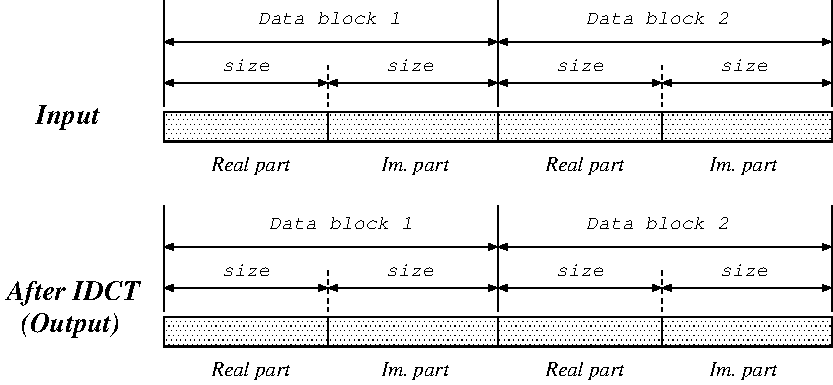
\includegraphics{fig/idct.pdf}
\end{center}
The Inverse Discrete Cosine Transformation II is given by
\begin{displaymath}
 x_{l} = \sqrt{\frac{2}{L}}c_{l}\sum_{k=0}^{L-1}
 X_{k}
 \cos\left\{\frac{\pi}{L} \left( k + \frac{1}{2} \right) l\right\},
\;\;\; l = 0, 1, \cdots, L
\end{displaymath}
where
 \begin{displaymath}
c_{l}= \begin{cases}
         \;\;1 & ( 1 \le l \le L - 1 ) \\
         \;\; 1 / \sqrt{2} & (l = 0)
        \end{cases}
 \end{displaymath}
\par
\end{qsection}

\begin{options}
        \argm{l}{L}{IDCT size}{256}
        \argm{c}{}{use complex number}{FALSE}
        \argm{d}{}{don't use FFT algorithm}{FALSE}
\end{options}

\begin{qsection}{EXAMPLE}
In this example, the IDCT is evaluated from a complex-valued data file
{\em data.f} in float format
(real part: 256 points, imaginary part: 256 points),
and the output is written to {\em data.idct}:
\begin{quote}
  \verb!idct data.f -l 256 -c > data.idct!
\end{quote}
\end{qsection}

\begin{qsection}{SEE ALSO}
 \hyperlink{fft}{fft},
 \hyperlink{dct}{dct}
\end{qsection}

% ----------------------------------------------------------------- %
%             The Speech Signal Processing Toolkit (SPTK)           %
%             developed by SPTK Working Group                       %
%             http://sp-tk.sourceforge.net/                         %
% ----------------------------------------------------------------- %
%                                                                   %
%  Copyright (c) 1984-2007  Tokyo Institute of Technology           %
%                           Interdisciplinary Graduate School of    %
%                           Science and Engineering                 %
%                                                                   %
%                1996-2016  Nagoya Institute of Technology          %
%                           Department of Computer Science          %
%                                                                   %
% All rights reserved.                                              %
%                                                                   %
% Redistribution and use in source and binary forms, with or        %
% without modification, are permitted provided that the following   %
% conditions are met:                                               %
%                                                                   %
% - Redistributions of source code must retain the above copyright  %
%   notice, this list of conditions and the following disclaimer.   %
% - Redistributions in binary form must reproduce the above         %
%   copyright notice, this list of conditions and the following     %
%   disclaimer in the documentation and/or other materials provided %
%   with the distribution.                                          %
% - Neither the name of the SPTK working group nor the names of its %
%   contributors may be used to endorse or promote products derived %
%   from this software without specific prior written permission.   %
%                                                                   %
% THIS SOFTWARE IS PROVIDED BY THE COPYRIGHT HOLDERS AND            %
% CONTRIBUTORS "AS IS" AND ANY EXPRESS OR IMPLIED WARRANTIES,       %
% INCLUDING, BUT NOT LIMITED TO, THE IMPLIED WARRANTIES OF          %
% MERCHANTABILITY AND FITNESS FOR A PARTICULAR PURPOSE ARE          %
% DISCLAIMED. IN NO EVENT SHALL THE COPYRIGHT OWNER OR CONTRIBUTORS %
% BE LIABLE FOR ANY DIRECT, INDIRECT, INCIDENTAL, SPECIAL,          %
% EXEMPLARY, OR CONSEQUENTIAL DAMAGES (INCLUDING, BUT NOT LIMITED   %
% TO, PROCUREMENT OF SUBSTITUTE GOODS OR SERVICES; LOSS OF USE,     %
% DATA, OR PROFITS; OR BUSINESS INTERRUPTION) HOWEVER CAUSED AND ON %
% ANY THEORY OF LIABILITY, WHETHER IN CONTRACT, STRICT LIABILITY,   %
% OR TORT (INCLUDING NEGLIGENCE OR OTHERWISE) ARISING IN ANY WAY    %
% OUT OF THE USE OF THIS SOFTWARE, EVEN IF ADVISED OF THE           %
% POSSIBILITY OF SUCH DAMAGE.                                       %
% ----------------------------------------------------------------- %
\hypertarget{ifft}{}
\name{ifft}{inverse FFT for complex sequence}{signal processing}

\begin{synopsis}
\item[ifft] [ --l $L$ ]  [ --\{ R $|$ I \} ] [ {\em infile} ] 
\end{synopsis}

\begin{qsection}{DESCRIPTION}
{\em ifft} calculates the Inverse Discrete Fourier Transform (IDFT) 
of complex-valued data from {\em infile} (or standard input), 
sending the results to standard output.
The input and output data is in float format, arranged as follows.
\begin{center}
 \leavevmode
 \includegraphics{fig/ifft.eps} 
\end{center}
\end{qsection}

\begin{options}
	\argm{l}{L}{FFT size power of 2}{256}
	\argm{R}{}{output only real part}{FALSE}
	\argm{I}{}{output only imaginary part}{FALSE}
\end{options}

\begin{qsection}{EXAMPLE}
In this example, the inverse DFT is evaluated from a data file
{\em data.f} in float format
(real part: 256 points, imaginary part: 256 points),
and the output is written to {\em data.ifft}:
\begin{quote}
  \verb!ifft data.f -l 256 > data.ifft!
\end{quote}
\end{qsection}

\begin{qsection}{SEE ALSO}
\hyperlink{fft}{fft},
\hyperlink{fft2}{fft2},
\hyperlink{fftr}{fftr},
\hyperlink{fftr2}{fftr2},
\hyperlink{ifftr}{ifftr}
\hyperlink{ifft2}{ifft2}
\end{qsection}

\name{ifft2}{$BJ#AG?tNs$N(B2$B<!859bB.5U%U!<%j%(JQ49(B}{none}

\begin{synopsis}
\item[ifft2] [ --l $L$ ] [ +r ] [ --t ] [ --c ] [ --q ] 
	     [ --\{ R $|$ I \} ] [ {\em infile} ]
\end{synopsis}

\begin{qsection}{DESCRIPTION}
{\em ifft2} $B$O!$J#AG?t7ONs$GM?$($i$l$k%G!<%?Ns$r(B{\em infile}$B$+$iFI$_9~$s$G(B
2$B<!855U%U!<%j%(JQ49$r9T$J$$!$7k2L$rI8=`=PNO$K=PNO$7$^$9!%(B  
{\em infile}$B$,;XDj$5$l$J$$;~$OI8=`F~NO$+$iFI$_9~$_$^$9!%(B
$B%G!<%?$N%U%)!<%^%C%H$O0J2<$NDL$j$G$9!%(B
\begin{center}
\leavevmode
\epsffile{fig/ifft2.eps}
\end{center}
\end{qsection}

\begin{options}
	\argm{l}{L}{$B%U!<%j%(JQ49$N%5%$%:!%(B2$B$N$Y$->h$G;XDj!%(B}{64}
	\argp{{\bf r}}{$BF~NO$r<B?t7?$H$9$k!%(B}{FALSE}
	\argm{t}{}{$B5U(BFFT$B$N7k2L$r(Btranspose$B$7$F=PNO!%!c(Bfft2 $B;2>H!d!%(B}{FALSE}
	\argm{c}{}{transpose$B$9$k:]!$6-3&$N(B1$B%G!<%?$rH?BPB&$+$i;}$C$F$-$F!$(B
		   $(L+1)\times (L+1)$ $B8D$N%G!<%?$r=PNO!%!c(Bfft2 $B;2>H!d!%(B}
		  {FALSE}
	\argm{q}{}{$B5U(BFFT$B$N7k2L$N:G=i$N(B1/4$B$N%G!<%?$N$_$r=PNO!%$3$N:](B c$B%*%W%7%g%s(B
		   $B$HF1MM$K!$6-3&$NJd=~$r9T$J$$!$(B
		   $(\frac{L}{2}+1)\times (\frac{L}{2}+1)$ $B8D$N%G!<%?$r(B
		   $B=PNO!%!c(Bfft2 $B;2>H!d!%(B}{FALSE}
	\argm{R}{}{$B<BIt$N$_$r=PNO!%(B}{FALSE}
	\argm{I}{}{$B5uIt$N$_$r=PNO!%(B}{FALSE}
\end{options}

\begin{qsection}{EXAMPLE}
float$B7A<0$N%U%!%$%k(B {\em data.f} $B$K$"$k(B2$B<!85J#AG?tNs$N(B $B5U(BDFT $B$r5a$a!$(B
{\em data.ifft2} $B$K=PNO$9$k(B:
\begin{quote}
  \verb!ifft2 -A < data.f > data.ifft2!
\end{quote}
\end{qsection}

\begin{qsection}{SEE ALSO}
 fft, fft2, ifft
\end{qsection}

% ----------------------------------------------------------------- %
%             The Speech Signal Processing Toolkit (SPTK)           %
%             developed by SPTK Working Group                       %
%             http://sp-tk.sourceforge.net/                         %
% ----------------------------------------------------------------- %
%                                                                   %
%  Copyright (c) 1984-2007  Tokyo Institute of Technology           %
%                           Interdisciplinary Graduate School of    %
%                           Science and Engineering                 %
%                                                                   %
%                1996-2013  Nagoya Institute of Technology          %
%                           Department of Computer Science          %
%                                                                   %
% All rights reserved.                                              %
%                                                                   %
% Redistribution and use in source and binary forms, with or        %
% without modification, are permitted provided that the following   %
% conditions are met:                                               %
%                                                                   %
% - Redistributions of source code must retain the above copyright  %
%   notice, this list of conditions and the following disclaimer.   %
% - Redistributions in binary form must reproduce the above         %
%   copyright notice, this list of conditions and the following     %
%   disclaimer in the documentation and/or other materials provided %
%   with the distribution.                                          %
% - Neither the name of the SPTK working group nor the names of its %
%   contributors may be used to endorse or promote products derived %
%   from this software without specific prior written permission.   %
%                                                                   %
% THIS SOFTWARE IS PROVIDED BY THE COPYRIGHT HOLDERS AND            %
% CONTRIBUTORS "AS IS" AND ANY EXPRESS OR IMPLIED WARRANTIES,       %
% INCLUDING, BUT NOT LIMITED TO, THE IMPLIED WARRANTIES OF          %
% MERCHANTABILITY AND FITNESS FOR A PARTICULAR PURPOSE ARE          %
% DISCLAIMED. IN NO EVENT SHALL THE COPYRIGHT OWNER OR CONTRIBUTORS %
% BE LIABLE FOR ANY DIRECT, INDIRECT, INCIDENTAL, SPECIAL,          %
% EXEMPLARY, OR CONSEQUENTIAL DAMAGES (INCLUDING, BUT NOT LIMITED   %
% TO, PROCUREMENT OF SUBSTITUTE GOODS OR SERVICES; LOSS OF USE,     %
% DATA, OR PROFITS; OR BUSINESS INTERRUPTION) HOWEVER CAUSED AND ON %
% ANY THEORY OF LIABILITY, WHETHER IN CONTRACT, STRICT LIABILITY,   %
% OR TORT (INCLUDING NEGLIGENCE OR OTHERWISE) ARISING IN ANY WAY    %
% OUT OF THE USE OF THIS SOFTWARE, EVEN IF ADVISED OF THE           %
% POSSIBILITY OF SUCH DAMAGE.                                       %
% ----------------------------------------------------------------- %
\hypertarget{ifftr}{}
\name{ifftr}{inverse FFT for real sequence}{signal processing}

\begin{synopsis}
 \item[ifftr] [ --l $L$ ] [ --m $M$ ] [ {\em infile} ]
\end{synopsis}

\begin{qsection}{DESCRIPTION}
{\em ifftr} calculates the Inverse Discrete Fourier Transform (IDFT)
of real-valued data from {\em infile} (or standard input),
sending the results to standard output.
The input and output data is in float format, arranged as follows.
\begin{displaymath}
\begin{array}{lll}
\mbox{Input sequence} & \overbrace{\framebox[4.5cm]{real part}}^{L} &
           \overbrace{\framebox[4.5cm]{imaginary part}}^{L} \\
                & \makebox[4.5cm]{0\hfill $L-1$} &
                \makebox[4.5cm]{0\hfill $L-1$}
\end{array}
\end{displaymath}
\begin{displaymath}
\begin{array}{lll}
\mbox{Output sequence} & 
\overbrace{\framebox[4.5cm]{$x_0, x_1, \ldots, x_{M}$}}^{L}  & \\
                & \makebox[4.5cm]{0\hfill $L-1$} &
\end{array}
\end{displaymath}
\end{qsection}

\begin{options}
 \argm{l}{L}{FFT size power of 2}{256}
 \argm{m}{M}{order of sequence}{L-1}
\end{options}

\begin{qsection}{EXAMPLE}
In this example, IDFT is evaluated from a data file
{\em data.f} in float format
(real part: 256 points, imaginary part: 256 points),
and the output is written to {\em data.ifftr}:
\begin{quote}
  \verb!ifftr data.f -l 256 > data.ifftr!
\end{quote}
\end{qsection}

\begin{qsection}{SEE ALSO}
\hyperlink{fft}{fft},
\hyperlink{fft2}{fft2},
\hyperlink{fftr}{fftr},
\hyperlink{fftr2}{fftr2},
\hyperlink{ifft}{ifft}
\hyperlink{ifft2}{ifft2}
\end{qsection}

% ----------------------------------------------------------------- %
%             The Speech Signal Processing Toolkit (SPTK)           %
%             developed by SPTK Working Group                       %
%             http://sp-tk.sourceforge.net/                         %
% ----------------------------------------------------------------- %
%                                                                   %
%  Copyright (c) 1984-2007  Tokyo Institute of Technology           %
%                           Interdisciplinary Graduate School of    %
%                           Science and Engineering                 %
%                                                                   %
%                1996-2013  Nagoya Institute of Technology          %
%                           Department of Computer Science          %
%                                                                   %
% All rights reserved.                                              %
%                                                                   %
% Redistribution and use in source and binary forms, with or        %
% without modification, are permitted provided that the following   %
% conditions are met:                                               %
%                                                                   %
% - Redistributions of source code must retain the above copyright  %
%   notice, this list of conditions and the following disclaimer.   %
% - Redistributions in binary form must reproduce the above         %
%   copyright notice, this list of conditions and the following     %
%   disclaimer in the documentation and/or other materials provided %
%   with the distribution.                                          %
% - Neither the name of the SPTK working group nor the names of its %
%   contributors may be used to endorse or promote products derived %
%   from this software without specific prior written permission.   %
%                                                                   %
% THIS SOFTWARE IS PROVIDED BY THE COPYRIGHT HOLDERS AND            %
% CONTRIBUTORS "AS IS" AND ANY EXPRESS OR IMPLIED WARRANTIES,       %
% INCLUDING, BUT NOT LIMITED TO, THE IMPLIED WARRANTIES OF          %
% MERCHANTABILITY AND FITNESS FOR A PARTICULAR PURPOSE ARE          %
% DISCLAIMED. IN NO EVENT SHALL THE COPYRIGHT OWNER OR CONTRIBUTORS %
% BE LIABLE FOR ANY DIRECT, INDIRECT, INCIDENTAL, SPECIAL,          %
% EXEMPLARY, OR CONSEQUENTIAL DAMAGES (INCLUDING, BUT NOT LIMITED   %
% TO, PROCUREMENT OF SUBSTITUTE GOODS OR SERVICES; LOSS OF USE,     %
% DATA, OR PROFITS; OR BUSINESS INTERRUPTION) HOWEVER CAUSED AND ON %
% ANY THEORY OF LIABILITY, WHETHER IN CONTRACT, STRICT LIABILITY,   %
% OR TORT (INCLUDING NEGLIGENCE OR OTHERWISE) ARISING IN ANY WAY    %
% OUT OF THE USE OF THIS SOFTWARE, EVEN IF ADVISED OF THE           %
% POSSIBILITY OF SUCH DAMAGE.                                       %
% ----------------------------------------------------------------- %
\hypertarget{ignorm}{}
\name{ignorm}{inverse gain normalization}{signal processing}
\begin{synopsis}
\item [ignorm] [ --m $M$ ] [ --g $G$ ] [ --c $C$ ] [ {\em infile} ]
\end{synopsis}

\begin{qsection}{DESCRIPTION}
{\em ignorm} reads normalized generalized cepstral coefficients
$c_\gamma(m)$ from {\em infile} (or standard input), 
and outputs the unnormalized coefficients to standard output.

Both input and output files are in float format.

To convert normalized generalized cepstral coefficients
$c_\gamma'(m)$ into not-normalized generalized cepstral coefficients
$c_\gamma(m)$, the following equation can be used.
\begin{displaymath}
c_\gamma(m) = \left( c_\gamma'(0) \right)^{\gamma} c_\gamma'(m), \qquad m>0
\end{displaymath}
Also, the gain $K = c_\gamma(0)$ is
\begin{displaymath}
c_\gamma(0) = \begin{cases} \;\; \displaystyle
          \frac{\Bigl(c_\gamma'(0)\Bigr)^{\gamma} - 1.0}{\gamma},
                & 0<|\gamma|\leq 1 \\ \;\; \displaystyle
          \log c_\gamma'(0),  & \gamma=0
        \end{cases}
\end{displaymath}
\end{qsection}

\begin{options}
        \argm{m}{M}{order of generalized cepstrum}{25}
        \argm{g}{G}{power parameter $\gamma$ of generalized cepstrum\\
                         $\gamma=G$}{0}
        \argm{c}{C}{power parameter $\gamma$ of generalized cepstrum\\
                        $\gamma =-1 / $(int)$ C$\\
                        $C$ must be $C \geq 1$}{}
\end{options}

\begin{qsection}{EXAMPLE}
In this example below,
normalized generalized cepstral coefficients in
float format are read from {\em data.ngcep} $(M=15, \gamma=-0.5)$,
and the not-normalized generalized cepstral coefficients
are output to {\em data.gcep}.
\begin{quote}
 \verb! ignorm -m 15 -c 2 < data.ngcep > data.gcep!
\end{quote} 
\end{qsection}

\begin{qsection}{SEE ALSO}
\hyperlink{gcep}{gcep},
\hyperlink{mgcep}{mgcep},
\hyperlink{gc2gc}{gc2gc},
\hyperlink{mgc2mgc}{mgc2mgc},
\hyperlink{freqt}{freqt}
\end{qsection}

%  ---------------------------------------------------------------  %
%            Speech Signal Processing Toolkit (SPTK)                %
%                      SPTK Working Group                           %
%                                                                   %
%                  Department of Computer Science                   %
%                  Nagoya Institute of Technology                   %
%                               and                                 %
%   Interdisciplinary Graduate School of Science and Engineering    %
%                  Tokyo Institute of Technology                    %
%                                                                   %
%                     Copyright (c) 1984-2007                       %
%                       All Rights Reserved.                        %
%                                                                   %
%  Permission is hereby granted, free of charge, to use and         %
%  distribute this software and its documentation without           %
%  restriction, including without limitation the rights to use,     %
%  copy, modify, merge, publish, distribute, sublicense, and/or     %
%  sell copies of this work, and to permit persons to whom this     %
%  work is furnished to do so, subject to the following conditions: %
%                                                                   %
%    1. The source code must retain the above copyright notice,     %
%       this list of conditions and the following disclaimer.       %
%                                                                   %
%    2. Any modifications to the source code must be clearly        %
%       marked as such.                                             %
%                                                                   %
%    3. Redistributions in binary form must reproduce the above     %
%       copyright notice, this list of conditions and the           %
%       following disclaimer in the documentation and/or other      %
%       materials provided with the distribution.  Otherwise, one   %
%       must contact the SPTK working group.                        %
%                                                                   %
%  NAGOYA INSTITUTE OF TECHNOLOGY, TOKYO INSTITUTE OF TECHNOLOGY,   %
%  SPTK WORKING GROUP, AND THE CONTRIBUTORS TO THIS WORK DISCLAIM   %
%  ALL WARRANTIES WITH REGARD TO THIS SOFTWARE, INCLUDING ALL       %
%  IMPLIED WARRANTIES OF MERCHANTABILITY AND FITNESS, IN NO EVENT   %
%  SHALL NAGOYA INSTITUTE OF TECHNOLOGY, TOKYO INSTITUTE OF         %
%  TECHNOLOGY, SPTK WORKING GROUP, NOR THE CONTRIBUTORS BE LIABLE   %
%  FOR ANY SPECIAL, INDIRECT OR CONSEQUENTIAL DAMAGES OR ANY        %
%  DAMAGES WHATSOEVER RESULTING FROM LOSS OF USE, DATA OR PROFITS,  %
%  WHETHER IN AN ACTION OF CONTRACT, NEGLIGENCE OR OTHER TORTUOUS   %
%  ACTION, ARISING OUT OF OR IN CONNECTION WITH THE USE OR          %
%  PERFORMANCE OF THIS SOFTWARE.                                    %
%                                                                   %
%  ---------------------------------------------------------------  %
%
\hypertarget{impulse}{}
\name{impulse}{generate impulse sequence}{signal processing}

\begin{synopsis}
\item[impulse] [ --l $L$ ] [ --n $N$ ]
\end{synopsis}

\begin{qsection}{DESCRIPTION}
{\em impulse} generates the unit impulse sequence of length $L$, 
sending the output to standard output. 
The output is in float format as follows.
\begin{displaymath}
\underbrace{1, 0, 0, \dots, 0}_{L}
\end{displaymath}

If both --l and --n options are given, the last one is used.
\end{qsection}

\begin{options}
	\argm{l}{L}{length of unit impulse\\
		    if $L < 0$ then endless sequence is generated.}{256}
	\argm{n}{N}{order of unit impulse}{255}
\end{options}

\begin{qsection}{EXAMPLE}
In the example below, an unit impulse sequence is passed through 
a digital filter and the results is presented on the screen.
\begin{quote}
 \verb!impulse | dfs -a 1 0.9 -b 1 2 1 | dmp +f!
\end{quote}
\end{qsection}

\begin{qsection}{SEE ALSO}
\hyperlink{step}{step},
\hyperlink{train}{train},
\hyperlink{ramp}{ramp},
\hyperlink{sin}{sin},
\hyperlink{nrand}{nrand}
\end{qsection}

\name{imsvq}{decoder of multi stage vector quantization}{VQ}

\begin{synopsis}
\item [imsvq] [ --l $L$ ] [ --n $N$ ] [ --s $S \;$ {\em cbfile} ] [ {\em infile} ]
\end{synopsis}

\begin{qsection}{DESCRIPTION}
The {\em imsvq} command reads the codebook indexes from {\em infile}
and sends the resulting multi stage output to the standard output.
The order of multi stage decoder is equal to the number of --s options
used.
\par
Input data is in int format, and output data is in float format.
\end{qsection}

\begin{options}
	\argm{l}{L}{length of vector}{26}
	\argm{n}{N}{order of vector}{L-1}
	\argm{s}{S \; cbfile}{codebook\\
		\begin{tabular}{ll}\\[-1zh]
		$S$ & codebook size\\
		$cbfile$ & codebook file \\
		\end{tabular}\\\hspace*{\fill}}{N/A N/A}
\end{options}

\begin{qsection}{EXAMPLE}
In the example below,
the decoded vector {\em data.ivq} is obtained
from the first stage codebook {\em cbfile1}
and the second stage codebook {\em cbfile2},
both of size 256, as well as from the index file {\em data.vq}.
\begin{quote}
\verb! imsvq -s 256 cbfile1 -s 256 cbfile2 < data.vq > data.ivq!
\end{quote}
\end{qsection}

\begin{qsection}{SEE ALSO}
msvq, ivq, vq
\end{qsection}

%  ---------------------------------------------------------------  %
%            Speech Signal Processing Toolkit (SPTK)                %
%                      SPTK Working Group                           %
%                                                                   %
%                  Department of Computer Science                   %
%                  Nagoya Institute of Technology                   %
%                               and                                 %
%   Interdisciplinary Graduate School of Science and Engineering    %
%                  Tokyo Institute of Technology                    %
%                                                                   %
%                     Copyright (c) 1984-2007                       %
%                       All Rights Reserved.                        %
%                                                                   %
%  Permission is hereby granted, free of charge, to use and         %
%  distribute this software and its documentation without           %
%  restriction, including without limitation the rights to use,     %
%  copy, modify, merge, publish, distribute, sublicense, and/or     %
%  sell copies of this work, and to permit persons to whom this     %
%  work is furnished to do so, subject to the following conditions: %
%                                                                   %
%    1. The source code must retain the above copyright notice,     %
%       this list of conditions and the following disclaimer.       %
%                                                                   %
%    2. Any modifications to the source code must be clearly        %
%       marked as such.                                             %
%                                                                   %
%    3. Redistributions in binary form must reproduce the above     %
%       copyright notice, this list of conditions and the           %
%       following disclaimer in the documentation and/or other      %
%       materials provided with the distribution.  Otherwise, one   %
%       must contact the SPTK working group.                        %
%                                                                   %
%  NAGOYA INSTITUTE OF TECHNOLOGY, TOKYO INSTITUTE OF TECHNOLOGY,   %
%  SPTK WORKING GROUP, AND THE CONTRIBUTORS TO THIS WORK DISCLAIM   %
%  ALL WARRANTIES WITH REGARD TO THIS SOFTWARE, INCLUDING ALL       %
%  IMPLIED WARRANTIES OF MERCHANTABILITY AND FITNESS, IN NO EVENT   %
%  SHALL NAGOYA INSTITUTE OF TECHNOLOGY, TOKYO INSTITUTE OF         %
%  TECHNOLOGY, SPTK WORKING GROUP, NOR THE CONTRIBUTORS BE LIABLE   %
%  FOR ANY SPECIAL, INDIRECT OR CONSEQUENTIAL DAMAGES OR ANY        %
%  DAMAGES WHATSOEVER RESULTING FROM LOSS OF USE, DATA OR PROFITS,  %
%  WHETHER IN AN ACTION OF CONTRACT, NEGLIGENCE OR OTHER TORTUOUS   %
%  ACTION, ARISING OUT OF OR IN CONNECTION WITH THE USE OR          %
%  PERFORMANCE OF THIS SOFTWARE.                                    %
%                                                                   %
%  ---------------------------------------------------------------  %
%
\hypertarget{interpolate}{}
\name{interpolate}{interpolation of data sequence}{signal processing}

\begin{synopsis}
\item[interpolate] [ --p $P$ ] [ --s $S$ ] [ --d ] [ {\em infile} ]
\end{synopsis}

\begin{qsection}{DESCRIPTION}
{\em interpolate} supplements a sequence of input data
from {\em infile} (or standard input)
by 0 or input data with interval $P$ and start number $S$,
sending the result to standard output.

If the input data is
\begin{displaymath}
 x(0), x(1), x(2), \dots
\end{displaymath}
then the output data is
\begin{displaymath}
\underbrace{0, 0, \dots, 0}_{S-1},\underbrace{x(0), 0, 0, \dots, 0}_{P},\underbrace{x(1), 0, 0, \dots, 0}_{P},x(2), \dots
\end{displaymath}
If the --d option is given, the output data is
\begin{displaymath}
\underbrace{0, 0, \dots, 0}_{S-1},\underbrace{x(0), x(0), x(0), \dots, x(0)}_{P},\underbrace{x(1), x(1), x(1), \dots, x(1)}_{P},x(2), \dots
\end{displaymath}
\par
Input and output data are in float format.
\end{qsection}

\begin{options}
        \argm{p}{P}{interpolation period}{10}
        \argm{s}{S}{start sample}{0}
        \argm{d}{}{pad input data rather than 0}{FALSE}
\end{options}

\begin{qsection}{EXAMPLE}
This example decimates input data from {\em data.f} file with interval 2,
interpolates 0 with interval 2, and then outputs it to {\em
data.di} file:
\begin{quote}
  \verb!decimate -p 2  < data.f | interpolate -p 2 > data.di!
\end{quote}
\end{qsection}

\begin{qsection}{SEE ALSO}
\hyperlink{decimate}{decimate}
\end{qsection}

% ----------------------------------------------------------------
%       Speech Signal Processing Toolkit (SPTK): version 3.0
%                      SPTK Working Group
% 
%                Department of Computer Science
%                Nagoya Institute of Technology
%                             and
%   Interdisciplinary Graduate School of Science and Engineering
%                Tokyo Institute of Technology
%                   Copyright (c) 1984-2000
%                     All Rights Reserved.
% 
% Permission is hereby granted, free of charge, to use and
% distribute this software and its documentation without
% restriction, including without limitation the rights to use,
% copy, modify, merge, publish, distribute, sublicense, and/or
% sell copies of this work, and to permit persons to whom this
% work is furnished to do so, subject to the following conditions:
% 
%   1. The code must retain the above copyright notice, this list
%      of conditions and the following disclaimer.
% 
%   2. Any modifications must be clearly marked as such.
%                                                                        
% NAGOYA INSTITUTE OF TECHNOLOGY, TOKYO INSITITUTE OF TECHNOLOGY,
% SPTK WORKING GROUP, AND THE CONTRIBUTORS TO THIS WORK DISCLAIM
% ALL WARRANTIES WITH REGARD TO THIS SOFTWARE, INCLUDING ALL
% IMPLIED WARRANTIES OF MERCHANTABILITY AND FITNESS, IN NO EVENT
% SHALL NAGOYA INSTITUTE OF TECHNOLOGY, TOKYO INSITITUTE OF
% TECHNOLOGY, SPTK WORKING GROUP, NOR THE CONTRIBUTORS BE LIABLE
% FOR ANY SPECIAL, INDIRECT OR CONSEQUENTIAL DAMAGES OR ANY
% DAMAGES WHATSOEVER RESULTING FROM LOSS OF USE, DATA OR PROFITS,
% WHETHER IN AN ACTION OF CONTRACT, NEGLIGENCE OR OTHER TORTIOUS
% ACTION, ARISING OUT OF OR IN CONNECTION WITH THE USE OR
% PERFORMANCE OF THIS SOFTWARE.
% ----------------------------------------------------------------
%
\hypertarget{ivq}{}
\name{ivq}{decoder of vector quantization}{vector quantization}

\begin{synopsis}
\item [ivq] [ --l $L$ ] [ --n $N$ ] {\em cbfile}  [ {\em infile} ] 
\end{synopsis}

\begin{qsection}{DESCRIPTION}
{\em ivq} decodes vector-quantized data from a sequence of codebook indexes
from {\em infile} (or standard input), 
using the codebook {\em cbfile}, 
sending the result to standard output. 
The decoded output vector format is
\begin{displaymath}
  c_i(0),c_i(1),\dots,c_i(L-1). 
\end{displaymath}

Input data is in int format, and output data is in float format.
\end{qsection}

\begin{options}
	\argm{l}{L}{length of vector}{26}
	\argm{n}{N}{order of vector}{L-1}
\end{options}

\begin{qsection}{EXAMPLE}
In the following example,
the decoded 25-th order output file {\em data.ivq} is obtained
through the index file {\em data.vq} and codebook {\em cbfile}.
\begin{quote}
\verb! ivq cbfile data.vq > data.ivq !
\end{quote}
\end{qsection}

\begin{qsection}{SEE ALSO}
\hyperlink{vq}{vq},
\hyperlink{imsvq}{imsvq},
\hyperlink{msvq}{msvq}
\end{qsection}

% ----------------------------------------------------------------- %
%             The Speech Signal Processing Toolkit (SPTK)           %
%             developed by SPTK Working Group                       %
%             http://sp-tk.sourceforge.net/                         %
% ----------------------------------------------------------------- %
%                                                                   %
%  Copyright (c) 1984-2007  Tokyo Institute of Technology           %
%                           Interdisciplinary Graduate School of    %
%                           Science and Engineering                 %
%                                                                   %
%                1996-2012  Nagoya Institute of Technology          %
%                           Department of Computer Science          %
%                                                                   %
% All rights reserved.                                              %
%                                                                   %
% Redistribution and use in source and binary forms, with or        %
% without modification, are permitted provided that the following   %
% conditions are met:                                               %
%                                                                   %
% - Redistributions of source code must retain the above copyright  %
%   notice, this list of conditions and the following disclaimer.   %
% - Redistributions in binary form must reproduce the above         %
%   copyright notice, this list of conditions and the following     %
%   disclaimer in the documentation and/or other materials provided %
%   with the distribution.                                          %
% - Neither the name of the SPTK working group nor the names of its %
%   contributors may be used to endorse or promote products derived %
%   from this software without specific prior written permission.   %
%                                                                   %
% THIS SOFTWARE IS PROVIDED BY THE COPYRIGHT HOLDERS AND            %
% CONTRIBUTORS "AS IS" AND ANY EXPRESS OR IMPLIED WARRANTIES,       %
% INCLUDING, BUT NOT LIMITED TO, THE IMPLIED WARRANTIES OF          %
% MERCHANTABILITY AND FITNESS FOR A PARTICULAR PURPOSE ARE          %
% DISCLAIMED. IN NO EVENT SHALL THE COPYRIGHT OWNER OR CONTRIBUTORS %
% BE LIABLE FOR ANY DIRECT, INDIRECT, INCIDENTAL, SPECIAL,          %
% EXEMPLARY, OR CONSEQUENTIAL DAMAGES (INCLUDING, BUT NOT LIMITED   %
% TO, PROCUREMENT OF SUBSTITUTE GOODS OR SERVICES; LOSS OF USE,     %
% DATA, OR PROFITS; OR BUSINESS INTERRUPTION) HOWEVER CAUSED AND ON %
% ANY THEORY OF LIABILITY, WHETHER IN CONTRACT, STRICT LIABILITY,   %
% OR TORT (INCLUDING NEGLIGENCE OR OTHERWISE) ARISING IN ANY WAY    %
% OUT OF THE USE OF THIS SOFTWARE, EVEN IF ADVISED OF THE           %
% POSSIBILITY OF SUCH DAMAGE.                                       %
% ----------------------------------------------------------------- %
\hypertarget{lbg}{}
\name{lbg}{LBG algorithm for vector quantizer design}{vector quantization}

\begin{synopsis}
\item [lbg] [ --l $L$ ] [ --n $N$ ] [ --t $T$ ] [ --s $S$ ] [ --e $E$ ]
        [ --f $F$ ] [ --i $I$ ] [ --m $M$ ] [ --S $s$ ] 
\item [\ ~~~~~] [ --c $C$ ] [ --d $D$ ] [ --r $R$ ] [ {\em indexfile} ] $<$ {\em infile}
\end{synopsis}

\begin{qsection}{DESCRIPTION}
{\em lbg} uses the LBG algorithm to train a codebook 
from a sequence of vectors from {\em infile} (or standard input), 
sending the result to standard output.

The input sequence consists of $T$ float vectors $\bx$, 
each of size $L$
\begin{displaymath} 
\bx(0), \bx(1), \dots, \bx(T-1). 
\end{displaymath}
The result is a codebook consisting of $E$ float vectors, 
each of length $L$,
\begin{displaymath}
\bC_E =\{ \bc_E(0), \bc_E(1), \dots, \bc_E(E-1) \}, 
\end{displaymath}
generated by the following algorithm.

\begin{description}
\item[\bf step.0~~~]
When an initial codebook $\bC_S$ is not assigned,
the initial codebook is obtained from the whole collection of
training data as follows,
\begin{displaymath}
\bc_1(0) = \frac{1}{T} \sum_{n=0}^{T-1} \bx(n)
\end{displaymath}
and the initial codebook with $S = 1$ is $\bC_1 = \{ \bc_1(0) \}$.

\item[\bf step.1~~~]
From codebook $\bC_{S}$ obtain $\bC_{2S}$.
For this step, the normalized random vector of size $L$ and the splitting factor
$R$ are used as follows,
\begin{displaymath}
\bc_{2S}(n)= \begin{cases}
\;\;\bc_S(n) + R \cdot \bm{\mathrm{rnd}} & ( 0 \le n \le S-1 ) \\
\;\;\bc_S(n-S) - R \cdot \bm{\mathrm{rnd}} & ( S \le n \le 2S-1 )
\end{cases}
\end{displaymath}
and we make $D_0 = \infty$ , $k = 0$.

\item[\bf step.2~~~]
First, make sure that $k \le I$ where $I$ is the maximum iterations
number specified by --i option.
If it is true, proceed to the following steps.
If not, then go to {\bf step.4}.
The present codebook $\bC_{2S}$ is now applied
to the training vectors.
After that, the mean Euclidean distance $D_k$ is evaluated
from every training vector and their corresponding code vector.
If the following condition 
\begin{displaymath}
\left|\frac{D_{k-1}-D_{k}}{D_{k}}\right| < D
\end{displaymath}
is met, then go to {\bf step.4}.
If it is not met, then go to {\bf step.3}.
The steps 0, 1, and 2 are illustrated in figure \ref{fig:lbg_step0},
\ref{fig:lbg_step1}, and \ref{fig:lbg_step2}, respectivelly.

\begin{figure}[tbp]
\begin{minipage}{0.5\hsize}
\begin{center}
\fbox{
  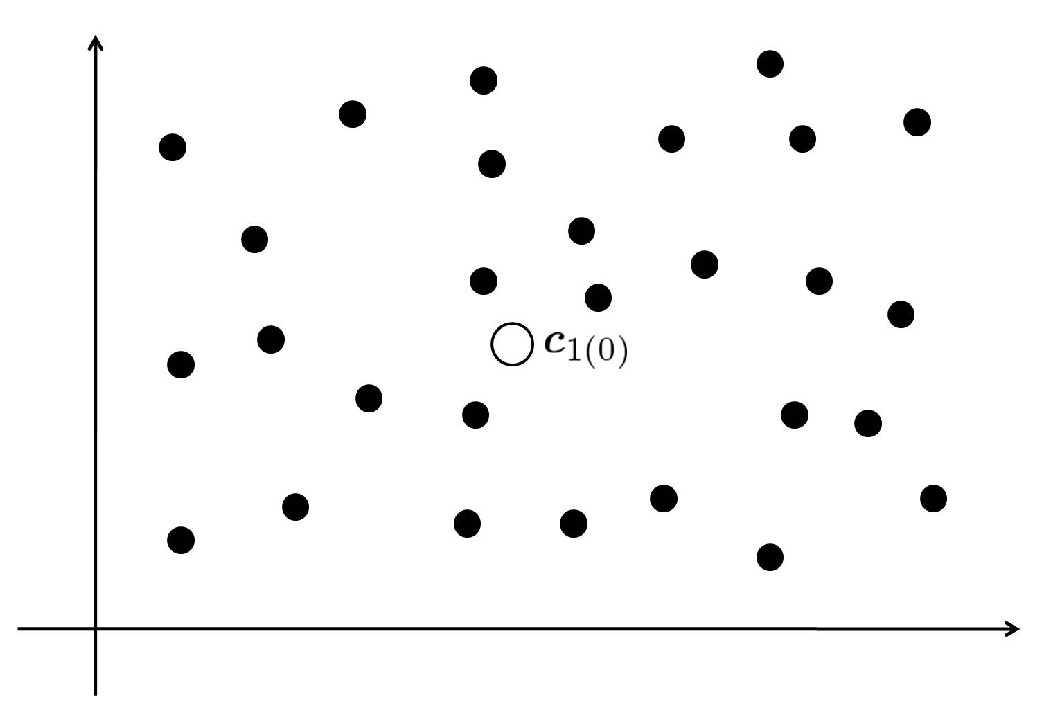
\includegraphics[width=5cm]{./fig/lbg_step0.eps}
}
\end{center}
\caption{{\bf step.0}: initialize codebook}
\label{fig:lbg_step0}
\end{minipage}
\begin{minipage}{0.5\hsize}
\begin{center}
\fbox{
  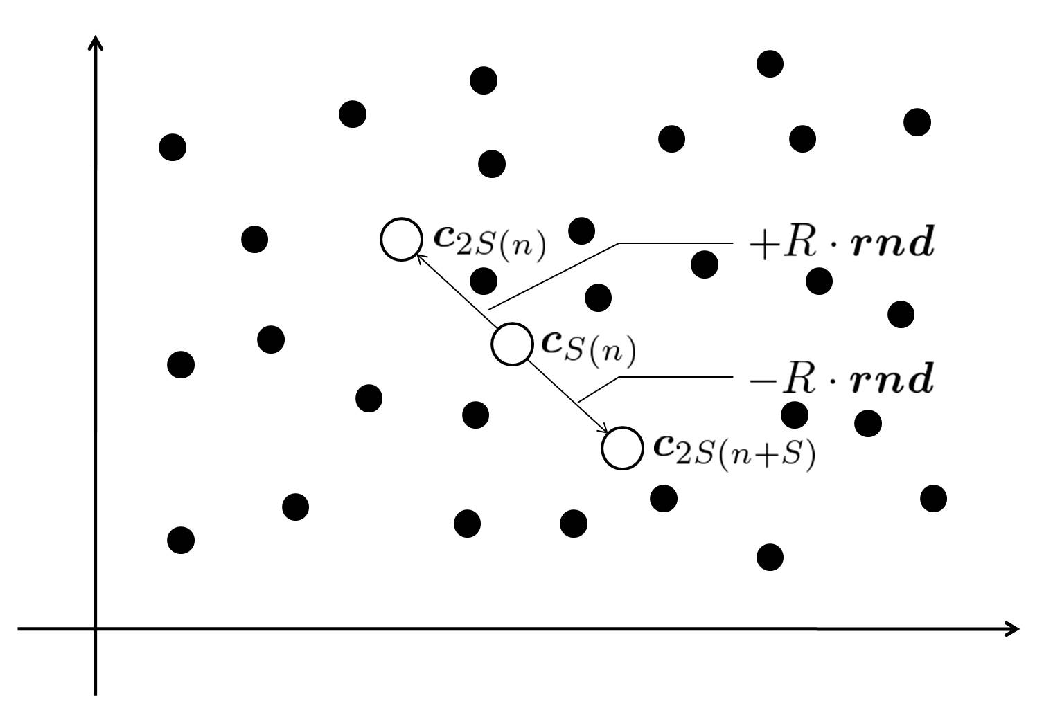
\includegraphics[width=5cm]{./fig/lbg_step1.eps}
}
\end{center}
\caption{{\bf step.1}: split codebook $\bC_{S}$ into $\bC_{2S}$}
\label{fig:lbg_step1}
\end{minipage}
\end{figure}
\begin{displaymath}
\left|\frac{D_{k-1}-D_{k}}{D_{k}}\right| < D
\end{displaymath}
\begin{figure}[tbp]
\begin{minipage}{0.5\hsize}
\begin{center}
\fbox{
  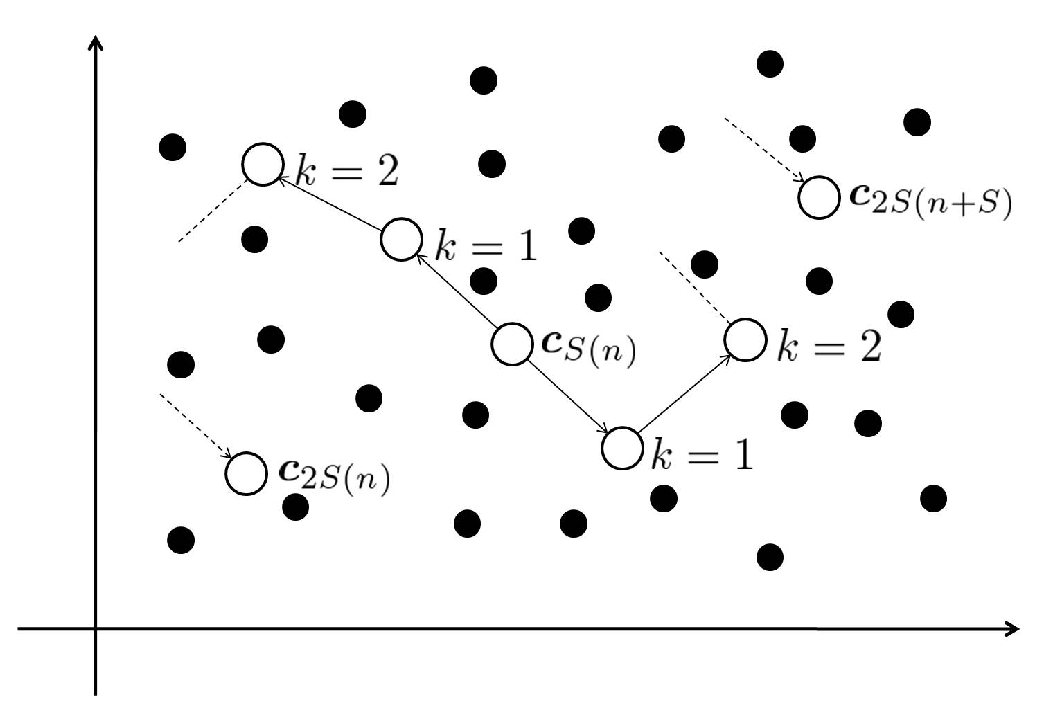
\includegraphics[width=5cm]{./fig/lbg_step2.eps}
}
\end{center}
\caption{{\bf step.2}: update codebook}
\label{fig:lbg_step2}
\end{minipage}
\end{figure}

\item[\bf step.3~~~]
Centroids are evaluated from the results obtained in {\bf step.2}.
Then, the codebook $\bC_{2S}$ is updated.
Also, if a cell has less than $M$ training vectors, then the corresponding
code vector is erased from the codebook,
and a new code vector is generated from either: 1) the code vector $\bc_{2S}(j)$  corresponding to the cell with more training vectors
, as follows.
\begin{displaymath}
\bc_{2S}(i) = \bc_{2S}(j) + R \cdot \bm{\mathrm{rnd}}
\end{displaymath}
Also, $\bc_{2S}(j)$ is modified as follows.
\begin{displaymath}
\bc_{2S}(j) = \bc_{2S}(j) - R \cdot \bm{\mathrm{rnd}}
\end{displaymath}
 2) the vector $\bp$, which internally divides
two centroids proportionally the number of training vectors for the cell.
They are split from the same parent centroid.
The vector $\bp$ is given by: 
\begin{displaymath}
\bp= \frac{n_{j}\bc_{2S}(i) + n_{i}\bc_{2S}(j)}{n_{i}+n_{j}},
\end{displaymath}
where $n_{i}$ and $n_{j}$ represent the number of training vectors for
the cells $\bc_{2S}(i) and \bc_{2S}(j)$, respectivelly.
The update method is as follows.
\begin{displaymath}
\bc_{2S}(i) = \bp + R \cdot \bm{\mathrm{rnd}},
\end{displaymath}
\begin{displaymath}
\bc_{2S}(j) = \bp- R \cdot \bm{\mathrm{rnd}}.
\end{displaymath}
If the number of traning vectors for the cell is less than $M$ when $k =
3$, the dividing vector $\bp$ and the update results are given as follows:

\begin{figure}[ht]
\setlength{\unitlength}{0.9mm}
\begin{center}
\begin{picture}(50,110)(20,0)
  \thicklines
  \put(60,105){\circle{10}}
  \put(49,105){\makebox(0,0){$k = 0$}}
  \put(80,108){\makebox(0,0){Parent centroid}} 
  \put(60,100){\vector(-2,-1){36}}
  \put(60,100){\vector(4,-3){28}}
  \put(24,79){\circle{6}}
  \put(88,76){\circle{6}}
  \put(15,79){\makebox(0,0){$k = 1$}}
  \put(97,76){\makebox(0,0){$k = 1$}}
  \put(24,76){\vector(-1,-2){15}}
  \put(88,73){\vector(3,-4){18}}
  \put(9,43){\circle{6}}
  \put(106,46){\circle{6}}
  \put(0,43){\makebox(0,0){$k = 2$}}
  \put(115,46){\makebox(0,0){$k = 2$}}
  \put(9,40){\vector(0,-1){15}}
  \put(106,43){\vector(-1,-3){5}}
  \put(9,22){\circle{6}}
  \put(101,25){\circle{6}}
  \put(0,22){\makebox(0,0){$k = 3$}}
  \put(110,25){\makebox(0,0){$k = 3$}}
  \put(9,15){\makebox(0,0){$\bc_{2S}(i)$}}
  \put(101,18){\makebox(0,0){$\bc_{2S}(j)$}}  
  \qbezier[90](12,22)(55,23)(98,25)
  \put(70,24){\circle*{20}}
  \thinlines
  \qbezier(12,22)(40,27)(67,24) 
  \qbezier(98,25)(85,27)(73,24)
  \put(70,24){\line(2,-1){24}}
  \put(94,12){\line(1,0){10}}
  \thicklines
  \put(40,27){\makebox(0,0)[b]{$n_i$}}
  \put(85,27){\makebox(0,0)[b]{$n_j$}}  
  \put(106,12){\makebox(0,0)[l]{dividing vector $\bp$}}
  \put(70,24){\vector(0,1){15}}
  \put(70,24){\vector(0,-1){15}}
  \put(70,42){\circle{6}}
  \put(70,6){\circle{6}}
  \put(69,34){\makebox(0,0)[r]{$+ R\cdot \bm{rnd}$}} 
  \put(69,14){\makebox(0,0)[r]{$- R\cdot \bm{rnd}$}}    
\end{picture}
\end{center}
\end{figure}

The type of split can be specified by the --c option.
After that, we assign $k=k+1$ and then go back to {\bf step.2}

\item[\bf step.4~~~]
If $2S = E$ then, end.
If not, then make $S$ = $2S$ and go back to {\bf step.1}.

\end{description}
\end{qsection}

\begin{options}
        \argm{l}{L}{length of vector}{26}
        \argm{n}{N}{order of vector}{L$-$1}
        \argm{t}{T}{number of training vector}{N/A}
        \argm{s}{S}{initial codebook size}{1}
        \argm{e}{E}{final codebook size}{256}
        \argm{f}{F}{initial codebook filename}{NULL}
        \argm{i}{I}{maximum number of iteration for centroid update}{1000} 
        \argm{m}{M}{minimum number of training vectors for each cell}{1}
        \argm{S}{s}{seed for normalized random vector}{1}
        \argm{c}{C}{type of exception procedure for centroid update \\
                    when the number of training vectors for the cell is less than $M$ \\
                    \begin{tabular}{ll} \\[-1ex]
                      $C=1$ & split the centroid with most training vectors\\
                      $C=2$ & split the vector which internally divide\\
                            & two centroids sharing the same parent centroid,\\
                            & in proportion to the number of training vectors for the cell.
                    \end{tabular}\\\hspace*{\fill}
                   }{1}
        \desc[1ex]{Usually, the options below do not need to be assigned.}
        \argm{d}{D}{end condition}{0.0001}
        \argm{r}{R}{splitting factor}{0.0001}
\end{options}

\begin{qsection}{EXAMPLE}
In the following example, a codebook of size 1024 is generated from
the 39-th order training vector {\em data.f} in float format.
It is also specified that the iterations for the centroid update are at most 100
 times, that each centroid contains at least 10 training vectors and that
 random vectors for the centroid update are generated with seed 5.
The output is written to {\em cbfile}.
\begin{quote}
\verb! lbg -n 39 -e 1024 -i 100 -m 10 -S 5 < data.f > cbfile!
\end{quote}
\end{qsection}

\begin{qsection}{SEE ALSO}
\hyperlink{vq}{vq},
\hyperlink{ivq}{ivq},
\hyperlink{msvq}{msvq}
\end{qsection}

% ----------------------------------------------------------------
%       Speech Signal Processing Toolkit (SPTK): version 3.0
%                      SPTK Working Group
% 
%                Department of Computer Science
%                Nagoya Institute of Technology
%                             and
%   Interdisciplinary Graduate School of Science and Engineering
%                Tokyo Institute of Technology
%                   Copyright (c) 1984-2000
%                     All Rights Reserved.
% 
% Permission is hereby granted, free of charge, to use and
% distribute this software and its documentation without
% restriction, including without limitation the rights to use,
% copy, modify, merge, publish, distribute, sublicense, and/or
% sell copies of this work, and to permit persons to whom this
% work is furnished to do so, subject to the following conditions:
% 
%   1. The code must retain the above copyright notice, this list
%      of conditions and the following disclaimer.
% 
%   2. Any modifications must be clearly marked as such.
%                                                                        
% NAGOYA INSTITUTE OF TECHNOLOGY, TOKYO INSITITUTE OF TECHNOLOGY,
% SPTK WORKING GROUP, AND THE CONTRIBUTORS TO THIS WORK DISCLAIM
% ALL WARRANTIES WITH REGARD TO THIS SOFTWARE, INCLUDING ALL
% IMPLIED WARRANTIES OF MERCHANTABILITY AND FITNESS, IN NO EVENT
% SHALL NAGOYA INSTITUTE OF TECHNOLOGY, TOKYO INSITITUTE OF
% TECHNOLOGY, SPTK WORKING GROUP, NOR THE CONTRIBUTORS BE LIABLE
% FOR ANY SPECIAL, INDIRECT OR CONSEQUENTIAL DAMAGES OR ANY
% DAMAGES WHATSOEVER RESULTING FROM LOSS OF USE, DATA OR PROFITS,
% WHETHER IN AN ACTION OF CONTRACT, NEGLIGENCE OR OTHER TORTIOUS
% ACTION, ARISING OUT OF OR IN CONNECTION WITH THE USE OR
% PERFORMANCE OF THIS SOFTWARE.
% ----------------------------------------------------------------
%
\name{levdur}{solve normal equation 
                    using Levinson-Durbin method}{signal processing}


\begin{synopsis}
 \item [levdur] [ --m $M$ ] [ {\em infile} ] 
\end{synopsis}

\begin{qsection}{DESCRIPTION}
This command evaluates the linear prediction coefficients
by solving a set of linear equations obtained from
the autocorrelation matrix.
From the assigned file, $M$ order autocorrelation matrix
\begin{displaymath}
  r(0),r(1),\ldots,r(M)
\end{displaymath}
is read and the linear system is solved by the Levinson-Durbin
algorithm.
\par
Input and output data are in float format.
\par
The linear prediction coefficients are the set of coefficients
$K, a(1), \ldots, a(M)$ of the all-pole digital filter
\begin{displaymath}
H(z) = \frac{K}{\displaystyle{1+\sum_{i=1}^{M}a(k)z^{-i}}}.
\end{displaymath}
The linear prediction coefficients are evaluated by solving
the following set of linear equations, which were obtained
through the autocorrelation method,
\begin{displaymath}
\left( \begin{array}{cccc}
        r(0) & r(1) & \cdots & r(M-1) \\
        r(1) & r(0) &        & \vdots \\
        \vdots &    & \ddots &         \\
        r(M-1) &    & \cdots & r(0)   \\
        \end{array} \right)
\left( \begin{array}{c}
	a(1) \\
	a(2) \\
	\vdots \\
	a(M) \\
	\end{array} \right)
= - \left( \begin{array}{c}
	r(1) \\
	r(2) \\
	\vdots \\
	r(M) \\
	\end{array} \right)
\end{displaymath}
The Durbin iterative and efficient algorithm is used
in the following taking advantage of the Toeplitz characteristic
of the autocorrelation matrix:
\begin{eqnarray}
E^{(0)}    &=& r(0) \\
k(i)       &=& \frac{\displaystyle{-r(i)-\sum_{j=1}^i a^{(i-1)}(j)r(i-j)}}
		{E^{(i-1)}} \label{eqn:lev_dur_k}\\
a^{(i)}(i) &=& k(i) \\
a^{(i)}(j) &=&  a^{(i-1)}(j) + k(i) a^{(i-1)}(i-j), 
		~~~~~1\leq j \leq i-1\\
E^{(i)}    &=& (1-k^2(i)) E^{(i-1)} \label{eqn:lev_dur_E}
\end{eqnarray}
Also, for $i=1,2,\ldots,M$, equations (\ref{eqn:lev_dur_k}) to
 (\ref{eqn:lev_dur_E}) are applied recursively,
and the gain $K$ is calculated as follows.
\begin{displaymath}
K = \sqrt{E^{(M)}}
\end{displaymath}
\end{qsection}

\begin{options}
	\argm{m}{M}{order of correlation}{25}
\end{options}

\begin{qsection}{EXAMPLE}
In this example, input data is read in float format from
{\em data.f} and linear prediction coefficients are written
to {\em data.lpc}:
\begin{quote}
 \verb!frame < data.f | window | acorr -m 25 | levdur > data.lpc!
\end{quote} 
\end{qsection}

\begin{qsection}{SEE ALSO}
 acorr, lpc
\end{qsection}

% ----------------------------------------------------------------- %
%             The Speech Signal Processing Toolkit (SPTK)           %
%             developed by SPTK Working Group                       %
%             http://sp-tk.sourceforge.net/                         %
% ----------------------------------------------------------------- %
%                                                                   %
%  Copyright (c) 1984-2007  Tokyo Institute of Technology           %
%                           Interdisciplinary Graduate School of    %
%                           Science and Engineering                 %
%                                                                   %
%                1996-2017  Nagoya Institute of Technology          %
%                           Department of Computer Science          %
%                                                                   %
% All rights reserved.                                              %
%                                                                   %
% Redistribution and use in source and binary forms, with or        %
% without modification, are permitted provided that the following   %
% conditions are met:                                               %
%                                                                   %
% - Redistributions of source code must retain the above copyright  %
%   notice, this list of conditions and the following disclaimer.   %
% - Redistributions in binary form must reproduce the above         %
%   copyright notice, this list of conditions and the following     %
%   disclaimer in the documentation and/or other materials provided %
%   with the distribution.                                          %
% - Neither the name of the SPTK working group nor the names of its %
%   contributors may be used to endorse or promote products derived %
%   from this software without specific prior written permission.   %
%                                                                   %
% THIS SOFTWARE IS PROVIDED BY THE COPYRIGHT HOLDERS AND            %
% CONTRIBUTORS "AS IS" AND ANY EXPRESS OR IMPLIED WARRANTIES,       %
% INCLUDING, BUT NOT LIMITED TO, THE IMPLIED WARRANTIES OF          %
% MERCHANTABILITY AND FITNESS FOR A PARTICULAR PURPOSE ARE          %
% DISCLAIMED. IN NO EVENT SHALL THE COPYRIGHT OWNER OR CONTRIBUTORS %
% BE LIABLE FOR ANY DIRECT, INDIRECT, INCIDENTAL, SPECIAL,          %
% EXEMPLARY, OR CONSEQUENTIAL DAMAGES (INCLUDING, BUT NOT LIMITED   %
% TO, PROCUREMENT OF SUBSTITUTE GOODS OR SERVICES; LOSS OF USE,     %
% DATA, OR PROFITS; OR BUSINESS INTERRUPTION) HOWEVER CAUSED AND ON %
% ANY THEORY OF LIABILITY, WHETHER IN CONTRACT, STRICT LIABILITY,   %
% OR TORT (INCLUDING NEGLIGENCE OR OTHERWISE) ARISING IN ANY WAY    %
% OUT OF THE USE OF THIS SOFTWARE, EVEN IF ADVISED OF THE           %
% POSSIBILITY OF SUCH DAMAGE.                                       %
% ----------------------------------------------------------------- %
\hypertarget{linear_intpl}{}
\name{linear\_intpl}{linear interpolation of data}{data processing}

\begin{synopsis}
\item[linear\_intpl] [ --l $L$ ] [ --m $M$ ] [ --x $x_{min} \; x_{max}$ ] 
[ --i $x_{min}$ ] [ --j $x_{max}$ ] [ {\em infile} ]
\end{synopsis}

\begin{qsection}{DESCRIPTION}
{\em linear\_intpl} reads a 2-dimensional input data sequence
from {\em infile} (or standard input) in which the $x$-axis values are
linearly interpolated by equally-spaced $L-1$ points, and outputs the
$y$-axis values.

If the input data is
\begin{displaymath}
   \begin{matrix}
	x_0, y_0 \\
	x_1, y_1 \\
	\vdots   \\
	x_K, y_K \\
	\end{matrix}
\end{displaymath}
then the output data will be
\begin{displaymath}
y_0, y_1, \dots, y_{L-1}
\end{displaymath}

\par
Input and output data are in float format.
\par
This command can also interpolate data sequence in wchich the $x$-axis
values are not equally-spaced,
such as digital filter characteristics.

\end{qsection}

\begin{options}
        \argm{l}{L}{output length}{256}
        \argm{m}{M}{number of interpolation points}{L-1}
        \argm{x}{x_{min} \; x_{max}}{minimum and maximum values of $x$-axis in 
        input data}{$0.0 \, 0.5$}
        \argm{i}{x_{min}}{minimum values of $x$-axis in input data}{$0.0$}
        \argm{j}{x_{max}}{maximum values of $x$-axis in input data}{$0.5$}
\end{options}

\begin{qsection}{EXAMPLE}
This example decimates input data from {\em data.f} file with interval 2,
interpolates 0 with interval 2, and then outputs it to {\em
data.di} file:

When input data {\em data.f} contains the following data,
\begin{eqnarray*}
&& 0, 2 \nonumber \\
&& 2, 2 \nonumber \\
&& 3, 0   \\
&& 5, 1 \nonumber \\
\end{eqnarray*}
this example linearly interpolates input data and outputs it to {\em data.intpl}
\begin{quote}
 \verb!linear_intpl -m 10 -x 0 5 < data.f > data.intpl!
\end{quote}
And the result is given by:
\begin{displaymath}
2, 2, 2, 2, 2, 1, 0, 0.25, 0.5, 0.75, 1
\end{displaymath}
\end{qsection}
% 
% \begin{qsection}{SEE ALSO}
%   decimate, interpolate
% \end{qsection}

% ----------------------------------------------------------------- %
%             The Speech Signal Processing Toolkit (SPTK)           %
%             developed by SPTK Working Group                       %
%             http://sp-tk.sourceforge.net/                         %
% ----------------------------------------------------------------- %
%                                                                   %
%  Copyright (c) 1984-2007  Tokyo Institute of Technology           %
%                           Interdisciplinary Graduate School of    %
%                           Science and Engineering                 %
%                                                                   %
%                1996-2010  Nagoya Institute of Technology          %
%                           Department of Computer Science          %
%                                                                   %
% All rights reserved.                                              %
%                                                                   %
% Redistribution and use in source and binary forms, with or        %
% without modification, are permitted provided that the following   %
% conditions are met:                                               %
%                                                                   %
% - Redistributions of source code must retain the above copyright  %
%   notice, this list of conditions and the following disclaimer.   %
% - Redistributions in binary form must reproduce the above         %
%   copyright notice, this list of conditions and the following     %
%   disclaimer in the documentation and/or other materials provided %
%   with the distribution.                                          %
% - Neither the name of the SPTK working group nor the names of its %
%   contributors may be used to endorse or promote products derived %
%   from this software without specific prior written permission.   %
%                                                                   %
% THIS SOFTWARE IS PROVIDED BY THE COPYRIGHT HOLDERS AND            %
% CONTRIBUTORS "AS IS" AND ANY EXPRESS OR IMPLIED WARRANTIES,       %
% INCLUDING, BUT NOT LIMITED TO, THE IMPLIED WARRANTIES OF          %
% MERCHANTABILITY AND FITNESS FOR A PARTICULAR PURPOSE ARE          %
% DISCLAIMED. IN NO EVENT SHALL THE COPYRIGHT OWNER OR CONTRIBUTORS %
% BE LIABLE FOR ANY DIRECT, INDIRECT, INCIDENTAL, SPECIAL,          %
% EXEMPLARY, OR CONSEQUENTIAL DAMAGES (INCLUDING, BUT NOT LIMITED   %
% TO, PROCUREMENT OF SUBSTITUTE GOODS OR SERVICES; LOSS OF USE,     %
% DATA, OR PROFITS; OR BUSINESS INTERRUPTION) HOWEVER CAUSED AND ON %
% ANY THEORY OF LIABILITY, WHETHER IN CONTRACT, STRICT LIABILITY,   %
% OR TORT (INCLUDING NEGLIGENCE OR OTHERWISE) ARISING IN ANY WAY    %
% OUT OF THE USE OF THIS SOFTWARE, EVEN IF ADVISED OF THE           %
% POSSIBILITY OF SUCH DAMAGE.                                       %
% ----------------------------------------------------------------- %
\hypertarget{lmadf}{}
\name[ref:acep-IEEESP,ref:LMA-IECE]{lmadf}%
{LMA digital filter for speech synthesis}{filters for speech synthesis}

\begin{synopsis}
\item [lmadf] [ --m $M$ ] [ --p $P$ ] [ --i $I$ ] [ --P $Pa$ ] [ --v ] [ --t ] [ --k ] 
      {\em cfile} [ {\em infile} ]
\end{synopsis}

\begin{qsection}{DESCRIPTION}
{\em lmadf} derives a Log Magnitude Approximation filter 
from cepstral coefficients $c(0),c(1),\ldots,c(M)$ in {\em cfile} 
and uses it to filter an excitation sequence 
from {\em infile} (or standard input) to synthesize speech data, 
sending the result to standard output.

Input and output data are in float format.

The LMA filter is an extremely precise approximation of the
exponential transfer function obtained from $M$-th order cepstral
coefficients $c(m)$ as follows.
\begin{displaymath}
H(z) = \exp \sum_{m=0}^{M} c(m) z^{-m}
\end{displaymath}
If we remove from the transfer function $H(z)$ the gain
$K=\exp c(0)$, then we obtain the following transfer function
\begin{displaymath}
D(z) = \exp \sum_{m=1}^{M} c(m) z^{-m},
\end{displaymath}
which can be realized using the basic FIR filter
\begin{displaymath}
F(z) = \sum_{m=1}^{M} c(m) z^{-m}
\end{displaymath}
as shown in figure \ref{fig:lmadflt_LMA}(a).
Also, as can be seen from figure \ref{fig:lmadflt_LMA}(b),
the basic filter $F(z)$ can be decomposed as follows
\begin{displaymath}
F(z) = F_1(z) + F_2(z)
\end{displaymath}
where 
\begin{align}
F_1(z) &= c(1) z^{-1} \notag \\
F_2(z) &= \sum_{m=2}^{M} c(m) z^{-m} \notag
\end{align}
By doing this decomposition, the accuracy of the approximation
is improved.
Also, the values of the coefficients $A_{4,l}$ are given
in table \ref{tbl:lmadflt_pade}
\par
\setcounter{figure}{0}
\begin{figure}[ht]
\setlength{\unitlength}{0.9mm}
\begin{center}
\begin{picture}(80,47)(20,0)
  \thicklines
  \multiput(20,30)(20,0){4}{\framebox(14,8){$F(z)$}}
  \multiput(34,34)(20,0){3}{\line(1,0){6}}
  \multiput(37,34)(20,0){3}{\circle*{1.4}}
  \put(94,34){\line(1,0){3}}
  \multiput(37,34)(20,0){4}{\line(0,-1){10}}
  \multiput(34,24)(20,0){4}{\line(1,0){6}}      %down triangle 
  \multiput(34,24)(20,0){4}{\line(2,-3){3}}
  \multiput(40,24)(20,0){4}{\line(-2,-3){3}}
  \put(10,34){\circle{4}}
  \put(10,34){\makebox(0,0){\scriptsize $+$}}
  \put(-6,34){\vector(1,0){14}}
  \put(-6,36){\makebox(0,0)[lb]{\small Input}}
  \put(12,34){\line(1,0){8}}
  \put(16,34){\circle*{1.4}}
  \put(16,34){\line(0,1){10}}
  \put(16,44){\vector(1,0){92}}
  \put(110,44){\circle{4}}
  \put(110,44){\makebox(0,0){\scriptsize $+$}}
  \put(112,44){\vector(1,0){14}}
  \put(112,46){\makebox(0,0)[lb]{\small Output}}
  \put(25,22){\makebox(0,0)[l]{$A_{4,1}$}}
  \put(45,22){\makebox(0,0)[l]{$A_{4,2}$}}
  \put(65,22){\makebox(0,0)[l]{$A_{4,3}$}}
  \put(85,22){\makebox(0,0)[l]{$A_{4,4}$}}

  \put(8.4,26){\makebox(0,0)[l]{\tiny $-$}}
  \put(16.4,26){\makebox(0,0)[l]{\tiny $-$}}

  \put(37,19.5){\line(0,-1){7.5}}
  \put(57,19.5){\line(0,-1){10.5}}
  \put(77,19.5){\line(0,-1){13.5}}
  \put(97,19.5){\line(0,-1){16.5}}

  \multiput(37,12)(20,-3){4}{\circle*{1.4}}
  \multiput(4,12)(4,-3){4}{\line(1,0){100}}

  \put(4,26){\line(0,-1){14}}
  \put(8,26){\line(0,-1){17}}
  \put(12,26){\line(0,-1){20}}
  \put(16,26){\line(0,-1){23}}

  \put(4,26){\vector(3,4){4.8}}
  \put(8,26){\vector(1,4){1.5}}
  \put(12,26){\vector(-1,4){1.5}}
  \put(16,26){\vector(-3,4){4.8}}

  \put(104,36){\line(0,-1){24}}
  \put(108,36){\line(0,-1){27}}
  \put(112,36){\line(0,-1){30}}
  \put(116,36){\line(0,-1){33}}

  \put(104,36){\vector(3,4){4.8}}
  \put(108,36){\vector(1,4){1.5}}
  \put(112,36){\vector(-1,4){1.5}}
  \put(116,36){\vector(-3,4){4.8}}
\end{picture}
\end{center}
\begin{center}
(a)
\end{center}

\vspace{2mm}
\setlength{\unitlength}{0.9mm}
\begin{center}
\begin{picture}(80,20)(10,0)
  \thicklines
  \put(15,0){\framebox(32,16){$R_L(F_1(z))$}}
  \put(57,0){\framebox(32,16){$R_L(F_2(z))$}}
  \put(0,8){\vector(1,0){15}}
  \put(47,8){\vector(1,0){10}}
  \put(89,8){\vector(1,0){15}}
  \put(2,10){\makebox(0,0)[lb]{$x(n)$}}
  \put(93,10){\makebox(0,0)[lb]{$y(n)$}}
  \put(0,17){\makebox(0,0)[lb]{Input}}
  \put(91,17){\makebox(0,0)[lb]{Output}}
\end{picture}
\end{center}
\begin{center}
(b)
\end{center}
\caption{\protect\parbox[t]{8cm}{
	(a)~~$R_L(F(z))\simeq D(z)$~~~$L=4$ \protect\\
	(b)~~2 level cascade realization\protect\\
        \hspace*{5mm} $R_L(F_1(z))\cdot R_L(F_2(z))\simeq D(z)$
}}
\label{fig:lmadflt_LMA}
\end{figure}

\setcounter{table}{0}
\begin{table}
        \caption{The values for the coefficients $A_{L,l}$}
        \label{tbl:lmadflt_coef}
        \setlength{\arrayrulewidth}{0.5pt}
        \renewcommand{\arraystretch}{1.2}
        \begin{center}
        \begin{tabular}{|c|c|c|} \hline
        $l$     & $A_{4,l}$			& $A_{5,l}$ \\ \hline
        1       & $4.999273\times 10^{-1}$	& $4.999391\times 10^{-1}$\\
        2       & $1.067005\times 10^{-1}$      & $1.107098\times 10^{-1}$\\
        3       & $1.170221\times 10^{-2}$      & $1.369984\times 10^{-2}$\\
        4       & $5.656279\times 10^{-4}$      & $9.564853\times 10^{-4}$\\
        5       &                               & $3.041721\times 10^{-5}$\\
      \hline
        \end{tabular}
        \end{center}
\label{tbl:lmadflt_pade}
\end{table}
\end{qsection}

\begin{options}
	\argm{m}{M}{order of cepstrum}{25}
	\argm{p}{P}{frame period}{100}
	\argm{i}{I}{interpolation period}{1}
	\argm{P}{Pa}{order of the Pad\'e approximation\\
                     $Pa$ should be $4$ or $5$}{4}
	\argm{k}{}{filtering without gain}{FALSE}
	\argm{v}{}{inverse filter}{FALSE}
	\argm{v}{}{transpose filter}{FALSE}
\end{options}

\begin{qsection}{EXAMPLE}
In this example, the excitation is generated from
the pitch data read in float format from {\em data.pitch},
passed through an LMA filter obtained from cepstrum file
{\em data.cep}, and the synthesized speech is written to
{\em data.syn}.
\begin{quote}
 \verb!excite < data.pitch | lmadf data.cep > data.syn!
\end{quote} 
\end{qsection}

\begin{qsection}{SEE ALSO}
\hyperlink{uels}{uels},
\hyperlink{acep}{acep},
\hyperlink{poledf}{poledf},
\hyperlink{ltcdf}{ltcdf},
\hyperlink{glsadf}{glsadf},
\hyperlink{mlsadf}{mlsadf},
\hyperlink{mglsadf}{mglsadf}
\end{qsection}

% ----------------------------------------------------------------- %
%             The Speech Signal Processing Toolkit (SPTK)           %
%             developed by SPTK Working Group                       %
%             http://sp-tk.sourceforge.net/                         %
% ----------------------------------------------------------------- %
%                                                                   %
%  Copyright (c) 1984-2007  Tokyo Institute of Technology           %
%                           Interdisciplinary Graduate School of    %
%                           Science and Engineering                 %
%                                                                   %
%                1996-2017  Nagoya Institute of Technology          %
%                           Department of Computer Science          %
%                                                                   %
% All rights reserved.                                              %
%                                                                   %
% Redistribution and use in source and binary forms, with or        %
% without modification, are permitted provided that the following   %
% conditions are met:                                               %
%                                                                   %
% - Redistributions of source code must retain the above copyright  %
%   notice, this list of conditions and the following disclaimer.   %
% - Redistributions in binary form must reproduce the above         %
%   copyright notice, this list of conditions and the following     %
%   disclaimer in the documentation and/or other materials provided %
%   with the distribution.                                          %
% - Neither the name of the SPTK working group nor the names of its %
%   contributors may be used to endorse or promote products derived %
%   from this software without specific prior written permission.   %
%                                                                   %
% THIS SOFTWARE IS PROVIDED BY THE COPYRIGHT HOLDERS AND            %
% CONTRIBUTORS "AS IS" AND ANY EXPRESS OR IMPLIED WARRANTIES,       %
% INCLUDING, BUT NOT LIMITED TO, THE IMPLIED WARRANTIES OF          %
% MERCHANTABILITY AND FITNESS FOR A PARTICULAR PURPOSE ARE          %
% DISCLAIMED. IN NO EVENT SHALL THE COPYRIGHT OWNER OR CONTRIBUTORS %
% BE LIABLE FOR ANY DIRECT, INDIRECT, INCIDENTAL, SPECIAL,          %
% EXEMPLARY, OR CONSEQUENTIAL DAMAGES (INCLUDING, BUT NOT LIMITED   %
% TO, PROCUREMENT OF SUBSTITUTE GOODS OR SERVICES; LOSS OF USE,     %
% DATA, OR PROFITS; OR BUSINESS INTERRUPTION) HOWEVER CAUSED AND ON %
% ANY THEORY OF LIABILITY, WHETHER IN CONTRACT, STRICT LIABILITY,   %
% OR TORT (INCLUDING NEGLIGENCE OR OTHERWISE) ARISING IN ANY WAY    %
% OUT OF THE USE OF THIS SOFTWARE, EVEN IF ADVISED OF THE           %
% POSSIBILITY OF SUCH DAMAGE.                                       %
% ----------------------------------------------------------------- %
\hypertarget{lpc}{}
\name{lpc}{LPC analysis using Levinson-Durbin method}{signal processing}

\begin{synopsis}
\item [lpc] [ --l $L$ ] [ --m $M$ ] [ --f $F$ ] [ {\em infile} ] 
\end{synopsis}

\begin{qsection}{DESCRIPTION}
{\em lpc} calculates linear prediction coefficients (LPC) 
from $L$-length framed windowed data from {\em infile} (or standard input), 
sending the result to standard output.

For each $L$-length input vector
\begin{displaymath}
  x(0),x(1),\ldots,x(L-1), 
\end{displaymath}
the autocorrelation function is calculated (see \hyperlink{acorr}{acorr}),
then the gain $K$ and the linear prediction coefficients
\begin{displaymath}
  K, a(1), \ldots, a(M)
\end{displaymath}
are calculated using the Levinson-Durbin algorithm (see \hyperlink{levdur}{levdur}). 

Input and output data are in float format.
\end{qsection}

\begin{options}
        \argm{l}{L}{frame length}{256}
        \argm{m}{M}{order of LPC}{25}
        \argm{f}{F}{mimimum value of the determinant of the normal matrix}{0.000001}
\end{options}

\begin{qsection}{EXAMPLE}
In this example, the 20-th order linear prediction analysis is applied
to input read from {\em data.f} in float format,
and the linear prediction coefficients are written to
{\em data.lpc}:
\begin{quote}
 \verb!frame < data.f | window | lpc -m 20 > data.lpc!
\end{quote} 
\end{qsection}

\begin{qsection}{SEE ALSO}
\hyperlink{acorr}{acorr},
\hyperlink{levdur}{levdur},
\hyperlink{lpc2par}{lpc2par},
\hyperlink{par2lpc}{par2lpc},
\hyperlink{lpc2c}{lpc2c},
\hyperlink{lpc2lsp}{lpc2lsp},
\hyperlink{lsp2lpc}{lsp2lpc}
\hyperlink{ltcdf}{ltcdf},
\hyperlink{lspdf}{lspdf}
\end{qsection}

% ----------------------------------------------------------------
%       Speech Signal Processing Toolkit (SPTK): version 3.0
%                      SPTK Working Group
% 
%                Department of Computer Science
%                Nagoya Institute of Technology
%                             and
%   Interdisciplinary Graduate School of Science and Engineering
%                Tokyo Institute of Technology
%                   Copyright (c) 1984-2000
%                     All Rights Reserved.
% 
% Permission is hereby granted, free of charge, to use and
% distribute this software and its documentation without
% restriction, including without limitation the rights to use,
% copy, modify, merge, publish, distribute, sublicense, and/or
% sell copies of this work, and to permit persons to whom this
% work is furnished to do so, subject to the following conditions:
% 
%   1. The code must retain the above copyright notice, this list
%      of conditions and the following disclaimer.
% 
%   2. Any modifications must be clearly marked as such.
%                                                                        
% NAGOYA INSTITUTE OF TECHNOLOGY, TOKYO INSITITUTE OF TECHNOLOGY,
% SPTK WORKING GROUP, AND THE CONTRIBUTORS TO THIS WORK DISCLAIM
% ALL WARRANTIES WITH REGARD TO THIS SOFTWARE, INCLUDING ALL
% IMPLIED WARRANTIES OF MERCHANTABILITY AND FITNESS, IN NO EVENT
% SHALL NAGOYA INSTITUTE OF TECHNOLOGY, TOKYO INSITITUTE OF
% TECHNOLOGY, SPTK WORKING GROUP, NOR THE CONTRIBUTORS BE LIABLE
% FOR ANY SPECIAL, INDIRECT OR CONSEQUENTIAL DAMAGES OR ANY
% DAMAGES WHATSOEVER RESULTING FROM LOSS OF USE, DATA OR PROFITS,
% WHETHER IN AN ACTION OF CONTRACT, NEGLIGENCE OR OTHER TORTIOUS
% ACTION, ARISING OUT OF OR IN CONNECTION WITH THE USE OR
% PERFORMANCE OF THIS SOFTWARE.
% ----------------------------------------------------------------
%
\hypertarget{lpc2c}{}
\name{lpc2c}{transform LPC to cepstrum}{speech parameter transformation}

\begin{synopsis}
 \item[lpc2c] [ --m $M_1$ ] [ --M $M_2$ ] [ {\em infile} ]
\end{synopsis}
\begin{qsection}{DESCRIPTION}
{\em lpc2c} calculates LPC cepstrum coefficients 
from linear prediction (LPC) coefficients 
from {\em infile} (or standard input), 
sending the result to standard output.
That is, when the input sequence is 
\begin{displaymath} 
   \sigma, a(1), a(2), \dots, a(p) 
\end{displaymath}
where
\begin{displaymath}
   H(z)=\frac{\sigma}{A(z)}=\frac{\sigma}{\displaystyle 1+\sum_{k=1}^P a(k) z^{-k}}
\end{displaymath}
then the LPC cepstrum coefficients are evaluated as follows.
\begin{displaymath}
   c(n) = \begin{cases}
 \;\; \ln(h),&n=0\\
 \;\; \displaystyle -a(n)=-\sum^{n-1}_{k=1}\frac{k}{n}c(k) a(n-k),&1\leq n\leq P\\ 
 \;\; \displaystyle -\sum_{k=n-P}^{n-1}\frac{k}{n}c(k) a(n-k),& n>P
\end{cases}
\end{displaymath}
And the sequence of cepstrum coefficients
\begin{displaymath}
   c(0), c(1), \dots, c(M)
\end{displaymath}
is outputed.
Input and output data are in float format.
\end{qsection}

\begin{options}
	\argm{m}{M_1}{order of LPC}{25}
	\argm{M}{M_2}{order of cepstrum}{25}
\end{options}

\begin{qsection}{EXAMPLE}
In the example below, a 10 order LPC analysis is undertaken after
passing the speech data {\em data.f} in float format through a window,
15 order LPC cepstrum coefficients are calculated,
and the result is written in {\em data.cep}.
\begin{quote}
 \verb!frame < data.f | window | lpc -m 10 |\!\\
 \verb!lpc2c -m 10 -M 15 > data.cep!
\end{quote}
\end{qsection}

\begin{qsection}{SEE ALSO}
\hyperlink{lpc}{lpc},
\hyperlink{gc2gc}{gc2gc},
\hyperlink{mgc2mgc}{mgc2mgc},
\hyperlink{freqt}{freqt}
\end{qsection}

% ----------------------------------------------------------------
%       Speech Signal Processing Toolkit (SPTK): version 3.0
%                      SPTK Working Group
% 
%                Department of Computer Science
%                Nagoya Institute of Technology
%                             and
%   Interdisciplinary Graduate School of Science and Engineering
%                Tokyo Institute of Technology
%                   Copyright (c) 1984-2000
%                     All Rights Reserved.
% 
% Permission is hereby granted, free of charge, to use and
% distribute this software and its documentation without
% restriction, including without limitation the rights to use,
% copy, modify, merge, publish, distribute, sublicense, and/or
% sell copies of this work, and to permit persons to whom this
% work is furnished to do so, subject to the following conditions:
% 
%   1. The code must retain the above copyright notice, this list
%      of conditions and the following disclaimer.
% 
%   2. Any modifications must be clearly marked as such.
%                                                                        
% NAGOYA INSTITUTE OF TECHNOLOGY, TOKYO INSITITUTE OF TECHNOLOGY,
% SPTK WORKING GROUP, AND THE CONTRIBUTORS TO THIS WORK DISCLAIM
% ALL WARRANTIES WITH REGARD TO THIS SOFTWARE, INCLUDING ALL
% IMPLIED WARRANTIES OF MERCHANTABILITY AND FITNESS, IN NO EVENT
% SHALL NAGOYA INSTITUTE OF TECHNOLOGY, TOKYO INSITITUTE OF
% TECHNOLOGY, SPTK WORKING GROUP, NOR THE CONTRIBUTORS BE LIABLE
% FOR ANY SPECIAL, INDIRECT OR CONSEQUENTIAL DAMAGES OR ANY
% DAMAGES WHATSOEVER RESULTING FROM LOSS OF USE, DATA OR PROFITS,
% WHETHER IN AN ACTION OF CONTRACT, NEGLIGENCE OR OTHER TORTIOUS
% ACTION, ARISING OUT OF OR IN CONNECTION WITH THE USE OR
% PERFORMANCE OF THIS SOFTWARE.
% ----------------------------------------------------------------
%
\hypertarget{lpc2lsp}{}
\name{lpc2lsp}{transform LPC to LSP}{speech parameter transformation}

\begin{synopsis}
\item [lpc2lsp] [ --m $M$ ] [ --s $S$ ] [ --k ] [ --l ] [ --o $O$ ] [ --n $N$ ]
		[ --p $P$ ] [ --q $Q$ ] [ --d $D$ ] 
\item [\ ~~~~~~~~] [ {\em infile} ] 
\end{synopsis}

\begin{qsection}{DESCRIPTION}
{\em lpc2lsp} calculates line spectral pair (LSP) coefficients 
from $M$-order linear prediction (LPC) coefficients 
from {\em infile} (or standard input),
sending the result to standard output.

The gain $K$ is included in the LPC input vectors
\begin{displaymath}
  K, a(1), \dots, a(M)
\end{displaymath}
but $K$ is not used in the calculation of the LSP coefficients.

The $M$-order polynomial linear prediction equation $A(z)$ is
\begin{displaymath}
  A_M(z) = 1 + \sum_{m=1}^M a(m) z^{-m}
\end{displaymath}
The PARCOR coefficients satisfy the following equations.
\begin{align}
  A_m(z) &= A_{m-1}(z) - k(m) B_{m-1}(z) \notag \\
  B_m(z) &= z^{-1} (B_{m-1}(z) - k(m) A_{m-1}(z)) \notag
\end{align}
Also, the initial conditions are set as follows,
\begin{displaymath}
  A_0(z) = 1, \qquad B_0(z) = z^{-1}
\end{displaymath}
When we are given the linear prediction polynomial equation
of $M$ order $A_M(z)$, and when the evaluation of $A_{M+1}(z)$
is obtained with the value of $k(M+1)$ equal to $1$ or $-1$, 
$P(z)$ and $Q(z)$ are defined as follow.
\begin{align}
  P(z) &= A_M(z) - B_M(z) \notag \\
  Q(z) &= A_M(z) + B_M(z) \notag
\end{align}
Making $k(M+1)$ equal to $\pm 1$ is means that,
with respect PARCOR coefficients,
the boundary condition for the glottis of the fixed vocal tract model
satisfies a perfect reflection characteristic.
Also, $A_M(z)$ can be expressed as
\begin{displaymath}
  A_M(z) = ( P(z) + Q(z) ) / 2.
\end{displaymath}
When we express $A_M(z)$ in this way,
$A_M(z)$ is stable.
That is for the roots of $A_M(z)=0$ to be all inside
the unit circle a necessary and sufficient condition is given
in the following.
\begin{itemize}
\item All of the roots of $P(z)=0$ and $Q(z)=0$ are on the unit circle
      line.
\item the roots of $P(z)=0$ and $Q(z)=0$ should be above the unit
      circle line and intercalate.
\end{itemize}
In other words, if  the roots of $P(z)=0$ and $Q(z)=0$ satisfy the
above condition, then $A_M(z)$ is stable.
\par
If we assume that $M$ is a even number, then
$P(z)$ and $Q(z)$ can be factorized as follows.
\begin{align}
  P(z) &= ( 1 - z^{-1} ) \prod_{i=2,4,\dots,M}
          ( 1 - 2 z^{-1} \cos \omega_i + z^{-2} ) \notag \\
  Q(z) &= ( 1 + z^{-1} ) \prod_{i=1,3,\dots,M-1}
          ( 1 - 2 z^{-1} \cos \omega_i + z^{-2} ) \notag
\end{align}
Also, the values of $\omega_i$ satisfy the following ordering condition.
\begin{displaymath}
  0 < \omega_1 < \omega_2 < \dots < \omega_{M-1} < \omega_M < \pi
\end{displaymath}
In the case, $M$ is odd number solution can be found in a similar way.
The coefficients $\omega_i$ obtained through factorization are called
LSP coefficients.
\end{qsection}

\begin{options}
	\argm{m}{M}{order of LPC}{25}
	\argm{s}{S}{sampling frequency (kHz)}{10}
	\argm{k}{}{output gain}{TRUE}
	\argm{l}{}{output log gain instead of linear gain}{FALSE}
	\argm{o}{O}{output format \\
		\begin{tabular}{ll} \\[-1ex]
			$0$ & normalized frequency $(0 \dots \pi)$ \\
			$1$ & normalized frequency $(0 \dots 0.5)$ \\
			$2$ & frequency (kHz) \\
			$3$ & frequency (Hz)  \\
		\end{tabular}\\\hspace*{\fill}}{0}
	\desc[0.6ex]{Usually, the options below do not need to be assigned.}
	\argm{n}{N}{split number of unit circle}{128}
	\argm{p}{P}{maximum number of interpolation for $P(z)$}{4}
	\argm{q}{Q}{maximum number of interpolation for $Q(z)$}{15}
	\argm{d}{D}{end condition of interpolation}{1e-06}
\end{options}

\begin{qsection}{EXAMPLE}
In the following example, speech data is read in float format from
{\em data.f}, 10 order LPC coefficients are calculated,
and the LSP coefficients are evaluated and written to {\em data.lsp}:
\begin{quote}
\verb!frame < data.f | window | lpc -m 10 |\!\\
\verb!lpc2lsp -m 10 > data.lsp!
\end{quote}
\end{qsection}

\begin{qsection}{SEE ALSO}
\hyperlink{lpc}{lpc},
\hyperlink{lsp2lpc}{lsp2lpc},
\hyperlink{lspdf}{lspdf}
\end{qsection}

%  ---------------------------------------------------------------  %
%            Speech Signal Processing Toolkit (SPTK)                %
%                      SPTK Working Group                           %
%                                                                   %
%                  Department of Computer Science                   %
%                  Nagoya Institute of Technology                   %
%                               and                                 %
%   Interdisciplinary Graduate School of Science and Engineering    %
%                  Tokyo Institute of Technology                    %
%                                                                   %
%                     Copyright (c) 1984-2007                       %
%                       All Rights Reserved.                        %
%                                                                   %
%  Permission is hereby granted, free of charge, to use and         %
%  distribute this software and its documentation without           %
%  restriction, including without limitation the rights to use,     %
%  copy, modify, merge, publish, distribute, sublicense, and/or     %
%  sell copies of this work, and to permit persons to whom this     %
%  work is furnished to do so, subject to the following conditions: %
%                                                                   %
%    1. The source code must retain the above copyright notice,     %
%       this list of conditions and the following disclaimer.       %
%                                                                   %
%    2. Any modifications to the source code must be clearly        %
%       marked as such.                                             %
%                                                                   %
%    3. Redistributions in binary form must reproduce the above     %
%       copyright notice, this list of conditions and the           %
%       following disclaimer in the documentation and/or other      %
%       materials provided with the distribution.  Otherwise, one   %
%       must contact the SPTK working group.                        %
%                                                                   %
%  NAGOYA INSTITUTE OF TECHNOLOGY, TOKYO INSTITUTE OF TECHNOLOGY,   %
%  SPTK WORKING GROUP, AND THE CONTRIBUTORS TO THIS WORK DISCLAIM   %
%  ALL WARRANTIES WITH REGARD TO THIS SOFTWARE, INCLUDING ALL       %
%  IMPLIED WARRANTIES OF MERCHANTABILITY AND FITNESS, IN NO EVENT   %
%  SHALL NAGOYA INSTITUTE OF TECHNOLOGY, TOKYO INSTITUTE OF         %
%  TECHNOLOGY, SPTK WORKING GROUP, NOR THE CONTRIBUTORS BE LIABLE   %
%  FOR ANY SPECIAL, INDIRECT OR CONSEQUENTIAL DAMAGES OR ANY        %
%  DAMAGES WHATSOEVER RESULTING FROM LOSS OF USE, DATA OR PROFITS,  %
%  WHETHER IN AN ACTION OF CONTRACT, NEGLIGENCE OR OTHER TORTUOUS   %
%  ACTION, ARISING OUT OF OR IN CONNECTION WITH THE USE OR          %
%  PERFORMANCE OF THIS SOFTWARE.                                    %
%                                                                   %
%  ---------------------------------------------------------------  %
%
\hypertarget{lpc2par}{}
\name{lpc2par}{transform LPC to PARCOR}{speech parameter transformation}

\begin{synopsis}
\item [lpc2par] [ --m $M$ ] [ --g $G$ ] [ --s ] [ {\em infile} ] 
\end{synopsis}

\begin{qsection}{DESCRIPTION}
{\em lpc2par} calculates PARCOR coefficients 
from $M$-th order linear prediction (LPC) coefficients 
from {\em infile} (or standard input), 
sending the result to standard output.

The LPC input format is
\begin{displaymath}
  K, a(1),\dots, a(M), 
\end{displaymath}
and the PARCOR output format is
\begin{displaymath}
  K, k(1),\dots, k(M).
\end{displaymath}
If the --s option is assigned, the stability of the filter is analyzed.
If the filter is stable, then 0 is returned.
If the filter is not stable, then 1 is returned to the standard output.
\par
Input and output data are in float format.
\par
The transformation from LPC coefficients to PARCOR coefficients
is undertaken as follows:
\begin{align} 
k(m) &= a^{(m)}(m) \notag \\
a^{(m-1)}(i) &= \frac{a^{(m)}(i)+a^{(m)}(m)a^{(m)}(m-i)}{1-k^2(m)}, \notag
\end{align}
where $1 \leq i \leq m-1$, $m=p, p-1, \dots, 1$.
The initial condition is
\begin{displaymath}  
a^{(M)}(m) = a(m), \qquad 1 \leq m \leq M.
\end{displaymath}
If we use the --g option, then the input contains normalized generalized
cepstral coefficients with power parameter $\gamma$
and the output contains the corresponding PARCOR coefficients.
In other words, the input is 
\begin{displaymath}
K,c_\gamma'(1),\dots,c_\gamma'(M)
\end{displaymath}
and the initial condition is
\begin{displaymath}
a^{(M)}(m) = \gamma c_\gamma'(M), \qquad 1 \leq m \leq M.
\end{displaymath}

Also with respect to the stability analysis,
the PARCOR coefficients are checked through the following equation.
\begin{displaymath}
-1 < k(m) < 1
\end{displaymath}
If this condition satisfy then the filter is stable.

\end{qsection}

\begin{options}
	\argm{m}{M}{order of LPC}{25}
	\argm{g}{G}{gamma of generalized cepstrum\\
			If $G>1.0$ then $\gamma=-1/G$.}{1}
	\argm{s}{}{check stable or unstable}{FALSE}
\end{options}

\begin{qsection}{EXAMPLE}
In the example below, a linear prediction analysis is
done in the input file {\em data.f} in float format,
the LPC coefficients are then transformed into PARCOR coefficients,
and the output is written to {\em data.rc}:
\begin{quote}
 \verb!frame +f < data.f | window | lpc | lpc2par > data.rc!
\end{quote} 
\end{qsection}

\begin{qsection}{SEE ALSO}
\hyperlink{acorr}{acorr},
\hyperlink{levdur}{levdur},
\hyperlink{lpc}{lpc},
\hyperlink{par2lpc}{par2lpc},
\hyperlink{ltcdf}{ltcdf}
\end{qsection}

\name{lsp2lpc}{transform LSP to LPC}{speech parameter transformation}

\begin{synopsis}
\item [lsp2lpc] [ --m $M$ ] [ --s $S$ ] [ --k ] [ --i $I$ ] [ {\em infile} ] 
\end{synopsis}

\begin{qsection}{DESCRIPTION}
The {\em lsp2lpc} command transforms LSP coefficients into
LPC coefficients.
If the gain is not assigned,
then its value is made equal to 1 as follows
\begin{displaymath}
	K = 1,a(1),\ldots,a(M).
 \end{displaymath}
\end{qsection}

\begin{options}
	\argm{m}{M}{order of LPC}{25}
	\argm{s}{S}{sampling frequency(kHz)}{10}
	\argm{k}{}{input & output gain}{TRUE}
	\argm{i}{I}{input format\\
		\begin{tabular}{ll} \\[-1zh]
			$0$ & normalized frequency $(0 \ldots \pi)$ \\
			$1$ & normalized frequency $(0 \ldots 0.5)$ \\
			$2$ & frequency (kHz) \\
			$3$ & frequency (Hz)  \\
		\end{tabular}\\\hspace*{\fill}}{0}
\end{options}

\begin{qsection}{EXAMPLE}
In the example below, 10 order LSP coefficients in float format
are read from file {\em data.lsp}, the linear prediction coefficients
are evalutated, and written to {\em data.lpc}:
\begin{quote}
\verb! lsp2lpc -m 10 < data.lsp > data.lpc!
\end{quote}
\end{qsection}

\begin{qsection}{SEE ALSO}
lpc, lpc2lsp
\end{qsection}

% ----------------------------------------------------------------- %
%             The Speech Signal Processing Toolkit (SPTK)           %
%             developed by SPTK Working Group                       %
%             http://sp-tk.sourceforge.net/                         %
% ----------------------------------------------------------------- %
%                                                                   %
%  Copyright (c) 1984-2007  Tokyo Institute of Technology           %
%                           Interdisciplinary Graduate School of    %
%                           Science and Engineering                 %
%                                                                   %
%                1996-2016  Nagoya Institute of Technology          %
%                           Department of Computer Science          %
%                                                                   %
% All rights reserved.                                              %
%                                                                   %
% Redistribution and use in source and binary forms, with or        %
% without modification, are permitted provided that the following   %
% conditions are met:                                               %
%                                                                   %
% - Redistributions of source code must retain the above copyright  %
%   notice, this list of conditions and the following disclaimer.   %
% - Redistributions in binary form must reproduce the above         %
%   copyright notice, this list of conditions and the following     %
%   disclaimer in the documentation and/or other materials provided %
%   with the distribution.                                          %
% - Neither the name of the SPTK working group nor the names of its %
%   contributors may be used to endorse or promote products derived %
%   from this software without specific prior written permission.   %
%                                                                   %
% THIS SOFTWARE IS PROVIDED BY THE COPYRIGHT HOLDERS AND            %
% CONTRIBUTORS "AS IS" AND ANY EXPRESS OR IMPLIED WARRANTIES,       %
% INCLUDING, BUT NOT LIMITED TO, THE IMPLIED WARRANTIES OF          %
% MERCHANTABILITY AND FITNESS FOR A PARTICULAR PURPOSE ARE          %
% DISCLAIMED. IN NO EVENT SHALL THE COPYRIGHT OWNER OR CONTRIBUTORS %
% BE LIABLE FOR ANY DIRECT, INDIRECT, INCIDENTAL, SPECIAL,          %
% EXEMPLARY, OR CONSEQUENTIAL DAMAGES (INCLUDING, BUT NOT LIMITED   %
% TO, PROCUREMENT OF SUBSTITUTE GOODS OR SERVICES; LOSS OF USE,     %
% DATA, OR PROFITS; OR BUSINESS INTERRUPTION) HOWEVER CAUSED AND ON %
% ANY THEORY OF LIABILITY, WHETHER IN CONTRACT, STRICT LIABILITY,   %
% OR TORT (INCLUDING NEGLIGENCE OR OTHERWISE) ARISING IN ANY WAY    %
% OUT OF THE USE OF THIS SOFTWARE, EVEN IF ADVISED OF THE           %
% POSSIBILITY OF SUCH DAMAGE.                                       %
% ----------------------------------------------------------------- %
\hypertarget{lsp2sp}{}
\name{lsp2sp}{transform LSP to spectrum}
{speech parameter transformation}

\begin{synopsis}
\item[lsp2sp] [ --m $M$ ] [ --s $S$ ] [ --l $L$ ] [ --L ] [ --k ] [ --q $Q$ ] [ --o $O$ ] [ {\em infile} ]
\end{synopsis}

\begin{qsection}{DESCRIPTION}
{\em lsp2sp} calculates the spectrum from the line spectral pairs (LSP)
from {\em infile} (or standard input),
sending the result to standard output.

Input and output data are in float format.

The LSP input format is
 \begin{displaymath}
  [ K ], l(1), \dots, l(M).
 \end{displaymath}
The spectrum can be obtained by
  \begin{displaymath}
   \mid H(\mathrm{e}^{-j\omega}) \mid = \frac{K}{\mid A_p(\mathrm{e}^{-j\omega}) \mid}.
  \end{displaymath}
where $\mid A_p(\mathrm{e}^{-j\omega}) \mid$ is given as follows:

When the order of LSP is even, 
  \begin{displaymath}
   \mid A_p(\mathrm{e}^{-j\omega}) \mid = \sqrt{ 2^M \left\{ \cos^2 \frac{\omega}{2}\prod_{i=1,3,\cdots,M-1}(\cos \omega - \cos l(i))^2 + \sin^2 \frac{\omega}{2}\prod_{i=2,4,\cdots,M}(\cos \omega - \cos l(i))^2 \right\} }.
  \end{displaymath}
When the order of LSP is odd,
 \begin{displaymath}
  \mid A_p(\mathrm{e}^{-j\omega}) \mid = \sqrt{ 2^{M-1} \left\{ \prod_{i=1,3,\cdots,M}(\cos \omega - \cos l(i))^2 + \sin^2 \omega \prod_{i=2,4,\cdots,M-1}(\cos \omega - \cos l(i))^2 \right\} }.
 \end{displaymath}
\end{qsection}

\begin{options}
 \argm{m}{M}{order of LSP}{10}
 \argm{s}{S}{sampling frequency (kHz)}{10.0}
	\argm{l}{L}{frame length}{256}
 \argm{L}{}{regard input log gain as linear one}{FALSE}
	\argm{q}{Q}{input format\\
        \begin{tabular}{ll} \\[-1ex]
            $0$ & normalized frequency $(0 \dots \pi)$ \\
            $1$ & normalized frequency $(0 \dots 0.5)$ \\
            $2$ & frequency (kHz) \\
            $3$ & frequency (Hz)  \\
        \end{tabular}\\\hspace*{\fill}}{0}
	\argm{o}{O}{output format\\
 \begin{tabular}{ll} \\[-1ex]
  $0$ & $20 \times \log |H(z)|$ \\
  $1$ & $\ln |H(z)|$ \\
  $2$ & $|H(z)|$ \\
  $3$ & $|H(z)|^{2}$ \\[1ex]
 \end{tabular}\\\hspace*{\fill}}{0}
\end{options}

\begin{qsection}{EXAMPLE}
The example below takes the 15-th order LSP from the file
 {\em data.cep} in float format, evaluates the spectrum,
 and presents it in the screen:
\begin{quote}
 \verb! lsp2sp -m 15 data.lsp | glogsp | xgr ! 
\end{quote}
\end{qsection}

\begin{qsection}{SEE ALSO}
\hyperlink{lpc2lsp}{lpc2lsp},
\hyperlink{lspcheck}{lspcheck}
\end{qsection}

% ----------------------------------------------------------------- %
%             The Speech Signal Processing Toolkit (SPTK)           %
%             developed by SPTK Working Group                       %
%             http://sp-tk.sourceforge.net/                         %
% ----------------------------------------------------------------- %
%                                                                   %
%  Copyright (c) 1984-2007  Tokyo Institute of Technology           %
%                           Interdisciplinary Graduate School of    %
%                           Science and Engineering                 %
%                                                                   %
%                1996-2011  Nagoya Institute of Technology          %
%                           Department of Computer Science          %
%                                                                   %
% All rights reserved.                                              %
%                                                                   %
% Redistribution and use in source and binary forms, with or        %
% without modification, are permitted provided that the following   %
% conditions are met:                                               %
%                                                                   %
% - Redistributions of source code must retain the above copyright  %
%   notice, this list of conditions and the following disclaimer.   %
% - Redistributions in binary form must reproduce the above         %
%   copyright notice, this list of conditions and the following     %
%   disclaimer in the documentation and/or other materials provided %
%   with the distribution.                                          %
% - Neither the name of the SPTK working group nor the names of its %
%   contributors may be used to endorse or promote products derived %
%   from this software without specific prior written permission.   %
%                                                                   %
% THIS SOFTWARE IS PROVIDED BY THE COPYRIGHT HOLDERS AND            %
% CONTRIBUTORS "AS IS" AND ANY EXPRESS OR IMPLIED WARRANTIES,       %
% INCLUDING, BUT NOT LIMITED TO, THE IMPLIED WARRANTIES OF          %
% MERCHANTABILITY AND FITNESS FOR A PARTICULAR PURPOSE ARE          %
% DISCLAIMED. IN NO EVENT SHALL THE COPYRIGHT OWNER OR CONTRIBUTORS %
% BE LIABLE FOR ANY DIRECT, INDIRECT, INCIDENTAL, SPECIAL,          %
% EXEMPLARY, OR CONSEQUENTIAL DAMAGES (INCLUDING, BUT NOT LIMITED   %
% TO, PROCUREMENT OF SUBSTITUTE GOODS OR SERVICES; LOSS OF USE,     %
% DATA, OR PROFITS; OR BUSINESS INTERRUPTION) HOWEVER CAUSED AND ON %
% ANY THEORY OF LIABILITY, WHETHER IN CONTRACT, STRICT LIABILITY,   %
% OR TORT (INCLUDING NEGLIGENCE OR OTHERWISE) ARISING IN ANY WAY    %
% OUT OF THE USE OF THIS SOFTWARE, EVEN IF ADVISED OF THE           %
% POSSIBILITY OF SUCH DAMAGE.                                       %
% ----------------------------------------------------------------- %
\hypertarget{lspcheck}{}
\name{lspcheck}{check stability and rearrange LSP}{speech parameter transformation}

\begin{synopsis}
\item [lspcheck] [ --m $M$ ] [ --s $S$ ] [ --k ] [ --i $I$ ] [ --o $O$ ]
		[ --r $R$] [ {\em infile} ] 
\end{synopsis}

\begin{qsection}{DESCRIPTION}
{\em lspcheck} tests the stability of the filter 
corresponding to the line spectral pair (LSP) coefficients 
from {\em infile} (or standard input), 
sending the result to standard output.

By default, the output is an ASCII report of the unstable frames.
However, if the --r option is given, 
the output is frames of coefficients 
that have been rearranged so the filter is stable.
\end{qsection}

\begin{options}
	\argm{m}{M}{order of LPC}{25}
	\argm{s}{S}{sampling frequency (kHz)}{10.0}
	\argm{k}{}{input \& output gain}{TRUE}
	\argm{i}{I}{input format}{0}
	\argm{o}{O}{output format \\
		\begin{tabular}{ll} \\[-1ex]
			$0$ & normalized frequency $(0 \ldots \pi)$ \\
			$1$ & normalized frequency $(0 \ldots 0.5)$ \\
			$2$ & frequency (kHz) \\
			$3$ & frequency (Hz)  \\
		\end{tabular}\\\hspace*{\fill}}{$I$}
	\argm{r}{R}{rearrange LSP\\
check the distance between two consecutive LSPs\\
and extend the distance (if it is smaller than $R\times \pi/M$)\\
$s.t.\hspace{0.5cm} 0 < R < 1$}{FALSE}
\end{options}

\begin{qsection}{EXAMPLE}
In the following example, 10-th order LSP coefficients are
read from {\em data.lsp} in float format,
stability is checked, the unstable coefficients are rearranged
so that they become stable, and the distance between two
consecutive LSPs are extended to $\pi /1000$ if
 it is smaller than $\pi /1000$, and the
 rearranged LSP coefficients are written to {\em data.lspr}:
\begin{quote}
\verb!lspcheck -m 10 -r 0.01 < data.lsp > data.lspr!
\end{quote}
\end{qsection}

\begin{qsection}{SEE ALSO}
\hyperlink{lpc}{lpc},
\hyperlink{lpc2lsp}{lpc2lsp},
\hyperlink{lsp2lpc}{lsp2lpc}
\end{qsection}

% ----------------------------------------------------------------- %
%             The Speech Signal Processing Toolkit (SPTK)           %
%             developed by SPTK Working Group                       %
%             http://sp-tk.sourceforge.net/                         %
% ----------------------------------------------------------------- %
%                                                                   %
%  Copyright (c) 1984-2007  Tokyo Institute of Technology           %
%                           Interdisciplinary Graduate School of    %
%                           Science and Engineering                 %
%                                                                   %
%                1996-2011  Nagoya Institute of Technology          %
%                           Department of Computer Science          %
%                                                                   %
% All rights reserved.                                              %
%                                                                   %
% Redistribution and use in source and binary forms, with or        %
% without modification, are permitted provided that the following   %
% conditions are met:                                               %
%                                                                   %
% - Redistributions of source code must retain the above copyright  %
%   notice, this list of conditions and the following disclaimer.   %
% - Redistributions in binary form must reproduce the above         %
%   copyright notice, this list of conditions and the following     %
%   disclaimer in the documentation and/or other materials provided %
%   with the distribution.                                          %
% - Neither the name of the SPTK working group nor the names of its %
%   contributors may be used to endorse or promote products derived %
%   from this software without specific prior written permission.   %
%                                                                   %
% THIS SOFTWARE IS PROVIDED BY THE COPYRIGHT HOLDERS AND            %
% CONTRIBUTORS "AS IS" AND ANY EXPRESS OR IMPLIED WARRANTIES,       %
% INCLUDING, BUT NOT LIMITED TO, THE IMPLIED WARRANTIES OF          %
% MERCHANTABILITY AND FITNESS FOR A PARTICULAR PURPOSE ARE          %
% DISCLAIMED. IN NO EVENT SHALL THE COPYRIGHT OWNER OR CONTRIBUTORS %
% BE LIABLE FOR ANY DIRECT, INDIRECT, INCIDENTAL, SPECIAL,          %
% EXEMPLARY, OR CONSEQUENTIAL DAMAGES (INCLUDING, BUT NOT LIMITED   %
% TO, PROCUREMENT OF SUBSTITUTE GOODS OR SERVICES; LOSS OF USE,     %
% DATA, OR PROFITS; OR BUSINESS INTERRUPTION) HOWEVER CAUSED AND ON %
% ANY THEORY OF LIABILITY, WHETHER IN CONTRACT, STRICT LIABILITY,   %
% OR TORT (INCLUDING NEGLIGENCE OR OTHERWISE) ARISING IN ANY WAY    %
% OUT OF THE USE OF THIS SOFTWARE, EVEN IF ADVISED OF THE           %
% POSSIBILITY OF SUCH DAMAGE.                                       %
% ----------------------------------------------------------------- %
\hypertarget{lspdf}{}
\name{lspdf}{LSP speech synthesis digital filter}{filters for speech synthesis}

\begin{synopsis}
\item [lspdf] [ --m $M$ ] [ --p $P$ ] [ --i $I$ ] [ --s $S$ ] [ --o $O$ ] 
              [ --k ] [ --l ] {\em lspfile} [ {\em infile} ] 
\end{synopsis}

\begin{qsection}{DESCRIPTION}
{\em lspdf} derives an LSP digital filter 
from the line spectral pair (LSP) coefficients in {\em lspfile} 
and uses it to filter an excitation sequence
from {\em infile} (or standard input) and synthesize speech data, 
sending the result to standard output.

Both input and output files are in float format.
\end{qsection}

\begin{options}
	\argm{m}{M}{order of coefficients}{25}
	\argm{p}{P}{frame period}{100}
	\argm{i}{I}{interpolation period}{1}
	\argm{k}{}{filtering without gain}{FALSE}
	\argm{l}{}{regard input as log gain}{FALSE}
\end{options}

\begin{qsection}{EXAMPLE}
In the example below, excitation is generated from the
pitch information given in {\em data.pitch} in float format.
This excitation is passed through the LSP synthesis filter
constructed from the LSP file {\em data.lsp},
and the synthesized speech is written to {\em data.syn}:
\begin{quote}
\verb! excite < data.pitch | lspdf data.lsp > data.syn!
\end{quote}
\end{qsection}

\begin{qsection}{SEE ALSO}
\hyperlink{lsp}{lsp},
\hyperlink{lpc2lsp}{lpc2lsp}
\end{qsection}

% ----------------------------------------------------------------- %
%             The Speech Signal Processing Toolkit (SPTK)           %
%             developed by SPTK Working Group                       %
%             http://sp-tk.sourceforge.net/                         %
% ----------------------------------------------------------------- %
%                                                                   %
%  Copyright (c) 1984-2007  Tokyo Institute of Technology           %
%                           Interdisciplinary Graduate School of    %
%                           Science and Engineering                 %
%                                                                   %
%                1996-2017  Nagoya Institute of Technology          %
%                           Department of Computer Science          %
%                                                                   %
% All rights reserved.                                              %
%                                                                   %
% Redistribution and use in source and binary forms, with or        %
% without modification, are permitted provided that the following   %
% conditions are met:                                               %
%                                                                   %
% - Redistributions of source code must retain the above copyright  %
%   notice, this list of conditions and the following disclaimer.   %
% - Redistributions in binary form must reproduce the above         %
%   copyright notice, this list of conditions and the following     %
%   disclaimer in the documentation and/or other materials provided %
%   with the distribution.                                          %
% - Neither the name of the SPTK working group nor the names of its %
%   contributors may be used to endorse or promote products derived %
%   from this software without specific prior written permission.   %
%                                                                   %
% THIS SOFTWARE IS PROVIDED BY THE COPYRIGHT HOLDERS AND            %
% CONTRIBUTORS "AS IS" AND ANY EXPRESS OR IMPLIED WARRANTIES,       %
% INCLUDING, BUT NOT LIMITED TO, THE IMPLIED WARRANTIES OF          %
% MERCHANTABILITY AND FITNESS FOR A PARTICULAR PURPOSE ARE          %
% DISCLAIMED. IN NO EVENT SHALL THE COPYRIGHT OWNER OR CONTRIBUTORS %
% BE LIABLE FOR ANY DIRECT, INDIRECT, INCIDENTAL, SPECIAL,          %
% EXEMPLARY, OR CONSEQUENTIAL DAMAGES (INCLUDING, BUT NOT LIMITED   %
% TO, PROCUREMENT OF SUBSTITUTE GOODS OR SERVICES; LOSS OF USE,     %
% DATA, OR PROFITS; OR BUSINESS INTERRUPTION) HOWEVER CAUSED AND ON %
% ANY THEORY OF LIABILITY, WHETHER IN CONTRACT, STRICT LIABILITY,   %
% OR TORT (INCLUDING NEGLIGENCE OR OTHERWISE) ARISING IN ANY WAY    %
% OUT OF THE USE OF THIS SOFTWARE, EVEN IF ADVISED OF THE           %
% POSSIBILITY OF SUCH DAMAGE.                                       %
% ----------------------------------------------------------------- %
\hypertarget{ltcdf}{}
\name{ltcdf}{all-pole lattice digital filter for speech synthesis}%
{filters for speech synthesis}

\begin{synopsis}
\item [ltcdf] [ --m $M$ ] [ --p $P$ ] [ --i $I$ ] [ --k ] {\em rcfile} 
	      [ {\em infile} ] 
\end{synopsis}

\begin{qsection}{DESCRIPTION}
{\em ltcdf} derives an all-pole lattice digital filter 
from PARCOR coefficients in {\em rcfile} 
and uses it to filter an excitation sequence
from {\em infile} (or standard input) and synthesize speech data, 
sending the result to standard output.

Both input and output files are in float format.
\end{qsection}

\begin{options}
	\argm{m}{M}{order of coefficients}{25}
	\argm{p}{P}{frame period}{100}
	\argm{i}{I}{interpolation period}{1}
	\argm{k}{}{filtering without gain}{FALSE}
\end{options}

\begin{qsection}{EXAMPLE}
In the example below, excitation is generated from the
pitch information given in {\em data.pitch} in float format.
This excitation is passed through the lattice filter
constructed from the LPC file {\em data.rc},
and the synthesized speech is written to {\em data.syn}:
\begin{quote}
 \verb!excite < data.pitch | ltcdf data.k > data.syn!
\end{quote} 
\end{qsection}

\begin{qsection}{SEE ALSO}
\hyperlink{lpc}{lpc},
\hyperlink{acorr}{acorr},
\hyperlink{levdur}{levdur},
\hyperlink{lpc2par}{lpc2par},
\hyperlink{par2lpc}{par2lpc},
\hyperlink{poledf}{poledf},
\hyperlink{zerodf}{zerodf},
\hyperlink{lspdf}{lspdf}
\end{qsection}

% ----------------------------------------------------------------- %
%             The Speech Signal Processing Toolkit (SPTK)           %
%             developed by SPTK Working Group                       %
%             http://sp-tk.sourceforge.net/                         %
% ----------------------------------------------------------------- %
%                                                                   %
%  Copyright (c) 1984-2007  Tokyo Institute of Technology           %
%                           Interdisciplinary Graduate School of    %
%                           Science and Engineering                 %
%                                                                   %
%                1996-2015  Nagoya Institute of Technology          %
%                           Department of Computer Science          %
%                                                                   %
% All rights reserved.                                              %
%                                                                   %
% Redistribution and use in source and binary forms, with or        %
% without modification, are permitted provided that the following   %
% conditions are met:                                               %
%                                                                   %
% - Redistributions of source code must retain the above copyright  %
%   notice, this list of conditions and the following disclaimer.   %
% - Redistributions in binary form must reproduce the above         %
%   copyright notice, this list of conditions and the following     %
%   disclaimer in the documentation and/or other materials provided %
%   with the distribution.                                          %
% - Neither the name of the SPTK working group nor the names of its %
%   contributors may be used to endorse or promote products derived %
%   from this software without specific prior written permission.   %
%                                                                   %
% THIS SOFTWARE IS PROVIDED BY THE COPYRIGHT HOLDERS AND            %
% CONTRIBUTORS "AS IS" AND ANY EXPRESS OR IMPLIED WARRANTIES,       %
% INCLUDING, BUT NOT LIMITED TO, THE IMPLIED WARRANTIES OF          %
% MERCHANTABILITY AND FITNESS FOR A PARTICULAR PURPOSE ARE          %
% DISCLAIMED. IN NO EVENT SHALL THE COPYRIGHT OWNER OR CONTRIBUTORS %
% BE LIABLE FOR ANY DIRECT, INDIRECT, INCIDENTAL, SPECIAL,          %
% EXEMPLARY, OR CONSEQUENTIAL DAMAGES (INCLUDING, BUT NOT LIMITED   %
% TO, PROCUREMENT OF SUBSTITUTE GOODS OR SERVICES; LOSS OF USE,     %
% DATA, OR PROFITS; OR BUSINESS INTERRUPTION) HOWEVER CAUSED AND ON %
% ANY THEORY OF LIABILITY, WHETHER IN CONTRACT, STRICT LIABILITY,   %
% OR TORT (INCLUDING NEGLIGENCE OR OTHERWISE) ARISING IN ANY WAY    %
% OUT OF THE USE OF THIS SOFTWARE, EVEN IF ADVISED OF THE           %
% POSSIBILITY OF SUCH DAMAGE.                                       %
% ----------------------------------------------------------------- %
\hypertarget{mc2b}{}
\name{mc2b}{transform mel-cepstrum to MLSA digital filter coefficients}%
{speech parameter transformation}

\begin{synopsis}
 \item [mc2b] [ --a $A$ ] [ --m $M$ ] [ {\em infile} ]
\end{synopsis}

\begin{qsection}{DESCRIPTION}
{\em mc2b} calculates MLSA filter coefficients $b(m)$ 
from mel-cepstral coefficients $c_\alpha(m)$ 
from {\em infile} (or standard input), 
sending the result to standard output.

Both input and output files are in float format.

The coefficients are given as follows:
\begin{displaymath}
b(m) = \begin{cases}
	  \;\; c_\alpha(M), & m=M \\
	  \;\; c_\alpha(m) - \alpha b(m+1), & 0 \leq m < M \\
	\end{cases}
\end{displaymath}
These coefficients $b(m)$ can be directly used in the
implementation of a MLSA filter.
{\em mc2b} implements the inverse transformation undertaken
by the command \hyperlink{b2mc}{b2mc}.
\end{qsection}

\begin{options}
	\argm{a}{A}{all-pass constant $\alpha$}{0.35}
	\argm{m}{M}{order of mel-cepstrum}{25}
\end{options}

\begin{qsection}{EXAMPLE}
In the example below, speech data is read in float format from {\em data.f},
a 12-th order mel-cepstral analysis is undertaken,
these mel-cepstral coefficients are transformed into
MLSA filter coefficients, and then the coefficients $b(m)$
are written to {\em data.b}:
\begin{quote}
 \verb!frame < data.f | window | mcep -m 12 |\ !\\
 \verb!mc2b -m 12 > data.b!
\end{quote} 
\end{qsection}

\begin{qsection}{SEE ALSO}
\hyperlink{mlsadf}{mlsadf},
\hyperlink{mglsadf}{mglsadf},
\hyperlink{b2mc}{b2mc},
\hyperlink{mcep}{mcep},
\hyperlink{mgcep}{mgcep},
\hyperlink{amcep}{amcep}
\end{qsection}

% ----------------------------------------------------------------- %
%             The Speech Signal Processing Toolkit (SPTK)           %
%             developed by SPTK Working Group                       %
%             http://sp-tk.sourceforge.net/                         %
% ----------------------------------------------------------------- %
%                                                                   %
%  Copyright (c) 1984-2007  Tokyo Institute of Technology           %
%                           Interdisciplinary Graduate School of    %
%                           Science and Engineering                 %
%                                                                   %
%                1996-2011  Nagoya Institute of Technology          %
%                           Department of Computer Science          %
%                                                                   %
% All rights reserved.                                              %
%                                                                   %
% Redistribution and use in source and binary forms, with or        %
% without modification, are permitted provided that the following   %
% conditions are met:                                               %
%                                                                   %
% - Redistributions of source code must retain the above copyright  %
%   notice, this list of conditions and the following disclaimer.   %
% - Redistributions in binary form must reproduce the above         %
%   copyright notice, this list of conditions and the following     %
%   disclaimer in the documentation and/or other materials provided %
%   with the distribution.                                          %
% - Neither the name of the SPTK working group nor the names of its %
%   contributors may be used to endorse or promote products derived %
%   from this software without specific prior written permission.   %
%                                                                   %
% THIS SOFTWARE IS PROVIDED BY THE COPYRIGHT HOLDERS AND            %
% CONTRIBUTORS "AS IS" AND ANY EXPRESS OR IMPLIED WARRANTIES,       %
% INCLUDING, BUT NOT LIMITED TO, THE IMPLIED WARRANTIES OF          %
% MERCHANTABILITY AND FITNESS FOR A PARTICULAR PURPOSE ARE          %
% DISCLAIMED. IN NO EVENT SHALL THE COPYRIGHT OWNER OR CONTRIBUTORS %
% BE LIABLE FOR ANY DIRECT, INDIRECT, INCIDENTAL, SPECIAL,          %
% EXEMPLARY, OR CONSEQUENTIAL DAMAGES (INCLUDING, BUT NOT LIMITED   %
% TO, PROCUREMENT OF SUBSTITUTE GOODS OR SERVICES; LOSS OF USE,     %
% DATA, OR PROFITS; OR BUSINESS INTERRUPTION) HOWEVER CAUSED AND ON %
% ANY THEORY OF LIABILITY, WHETHER IN CONTRACT, STRICT LIABILITY,   %
% OR TORT (INCLUDING NEGLIGENCE OR OTHERWISE) ARISING IN ANY WAY    %
% OUT OF THE USE OF THIS SOFTWARE, EVEN IF ADVISED OF THE           %
% POSSIBILITY OF SUCH DAMAGE.                                       %
% ----------------------------------------------------------------- %
\hypertarget{mcep}{}
\name[ref:mcep-IEICE,ref:amcep-ICASSP92]{mcep}{mel cepstral analysis}%
{speech analysis}

\begin{synopsis}
\item [mcep] [ --a $A$ ] [ --m $M$ ] [ --l $L$ ] [ --q $Q$ ] [ --i $I$ ] [ --j $J$ ] 
	     [ --d $D$ ] [ --e $E$ ] [ --f $F$ ]
\item [\ ~~~~~~~~] [ {\em infile} ]
\end{synopsis}

\begin{qsection}{DESCRIPTION}
{\em mcep} uses mel-cepstral analysis 
to calculate mel-cepstral coefficients $c_{\alpha}(m)$ 
from $L$-length framed windowed data from {\em infile} (or standard input), 
sending the result to standard output.

Input and output data are in float format.

In the mel-cepstral analysis, the spectrum of the speech signal
is modeled by $M$-th order mel-cepstral coefficients $c_{\alpha}(m)$
as follows.
\begin{displaymath}
H(z) = \exp \sum_{m=0}^M c_{\alpha}(m) \tilde{z}^{-m} 
\end{displaymath}
For this command ``mcep'', it is applied a cost function
based on the unbiased estimation log spectrum method.
The variable $\tilde{z}^{-1}$ can be expressed as the following
first order all-pass function
\begin{displaymath}
\tilde{z}^{-1} = \frac{z^{-1}-\alpha}{1-\alpha z^{-1}}.
\end{displaymath}
The phase characteristic is given by the variable $\alpha$.
For a sampling rate 16 kHz, $\alpha$ is made equal to $0.42$.
For a sampling rate 10 kHz, $\alpha$ is made equal to $0.35$.
For a sampling rate 8 kHz, $\alpha$ is made equal to $0.31$.
By making these choices for $\alpha$,
the mel-scale becomes the good approximation to human
sensitivity to the loudness speech sound.

The Newton-Raphson method is used to minimize the cost function
when evaluating mel-cepstral coefficients.
\end{qsection}

\begin{options}
	\argm{a}{A}{all-pass constant $\alpha$}{0.35}
	\argm{m}{M}{order of mel cepstrum}{25}
	\argm{l}{L}{frame length}{256}
    \argm{q}{Q}{input data style\\
        \begin{tabular}{ll} \\[-1ex]
            $Q=0$ & windowed data sequence \\
            $Q=1$ & $20 \times \log |f(w)|$ \\
            $Q=2$ & $\ln |f(w)|$ \\
            $Q=3$ & $|f(w)|$ \\
            $Q=4$ & $|f(w)|^2$ \\[1ex]
        \end{tabular}\\\hspace*{\fill}}{0}
	\desc[1ex]{Usually, the options below do not need to be assigned.}
	\argm{i}{I}{minimum iteration of Newton-Raphson method}{2}
	\argm{j}{J}{maximum iteration of Newton-Raphson method}{30}
	\argm{d}{D}{end condition of Newton-Raphson}{0.001}
	\argm{e}{E}{small value added to periodgram}{0.0}
	\argm{f}{F}{minimum value of the determinant of the normal matrix}{0.000001}
\end{options}

\begin{qsection}{EXAMPLE}
Speech data is read in float format from {\em data.f} and 
analyzed, and mel-cepstral coefficients are written to {\em data.mcep}:
\begin{quote}
 \verb!frame +f < data.f | window | mcep > data.mcep !
\end{quote}
\begin{quote}
 \verb!frame +f < data.f | window | fftr -A -H | mcep -q 3 > data.mcep !
\end{quote}
\end{qsection}

\begin{qsection}{SEE ALSO}
\hyperlink{uels}{uels},
\hyperlink{gcep}{gcep},
\hyperlink{mgcep}{mgcep},
\hyperlink{mlsadf}{mlsadf}
\end{qsection}

% ----------------------------------------------------------------- %
%             The Speech Signal Processing Toolkit (SPTK)           %
%             developed by SPTK Working Group                       %
%             http://sp-tk.sourceforge.net/                         %
% ----------------------------------------------------------------- %
%                                                                   %
%  Copyright (c) 1984-2007  Tokyo Institute of Technology           %
%                           Interdisciplinary Graduate School of    %
%                           Science and Engineering                 %
%                                                                   %
%                1996-2013  Nagoya Institute of Technology          %
%                           Department of Computer Science          %
%                                                                   %
% All rights reserved.                                              %
%                                                                   %
% Redistribution and use in source and binary forms, with or        %
% without modification, are permitted provided that the following   %
% conditions are met:                                               %
%                                                                   %
% - Redistributions of source code must retain the above copyright  %
%   notice, this list of conditions and the following disclaimer.   %
% - Redistributions in binary form must reproduce the above         %
%   copyright notice, this list of conditions and the following     %
%   disclaimer in the documentation and/or other materials provided %
%   with the distribution.                                          %
% - Neither the name of the SPTK working group nor the names of its %
%   contributors may be used to endorse or promote products derived %
%   from this software without specific prior written permission.   %
%                                                                   %
% THIS SOFTWARE IS PROVIDED BY THE COPYRIGHT HOLDERS AND            %
% CONTRIBUTORS "AS IS" AND ANY EXPRESS OR IMPLIED WARRANTIES,       %
% INCLUDING, BUT NOT LIMITED TO, THE IMPLIED WARRANTIES OF          %
% MERCHANTABILITY AND FITNESS FOR A PARTICULAR PURPOSE ARE          %
% DISCLAIMED. IN NO EVENT SHALL THE COPYRIGHT OWNER OR CONTRIBUTORS %
% BE LIABLE FOR ANY DIRECT, INDIRECT, INCIDENTAL, SPECIAL,          %
% EXEMPLARY, OR CONSEQUENTIAL DAMAGES (INCLUDING, BUT NOT LIMITED   %
% TO, PROCUREMENT OF SUBSTITUTE GOODS OR SERVICES; LOSS OF USE,     %
% DATA, OR PROFITS; OR BUSINESS INTERRUPTION) HOWEVER CAUSED AND ON %
% ANY THEORY OF LIABILITY, WHETHER IN CONTRACT, STRICT LIABILITY,   %
% OR TORT (INCLUDING NEGLIGENCE OR OTHERWISE) ARISING IN ANY WAY    %
% OUT OF THE USE OF THIS SOFTWARE, EVEN IF ADVISED OF THE           %
% POSSIBILITY OF SUCH DAMAGE.                                       %
% ----------------------------------------------------------------- %
\hypertarget{merge}{}
\name{merge}{data merge}{data operation}

\begin{synopsis}
 \item[merge] [ --s $S$ ] [ --l $L_1$ ] [ --n $N_1$ ] [ --L $L_2$ ]
 [ --N $N_2$ ]
 \item[\ ~~~]  [ --o ] [ +{\em type} ] {\em file1} [ {\em infile} ] 
\end{synopsis}

\begin{qsection}{DESCRIPTION}
{\em merge} merges, on a frame-by-frame basis, data from {\em file1} 
into the data from {\em infile} (or standard input), 
sending the result to standard output, as described below.

\hspace{1cm}\includegraphics{fig/merge.eps}
\end{qsection}

\begin{options}
	\argm{s}{S}{insert point}{0}
	\argm{l}{L_1}{frame length of input data}{25}
	\argm{n}{N_1}{order of input data}{$L_1-1$}
	\argm{L}{L_2}{frame length of insert data}{10}
	\argm{N}{N_2}{order of insert data}{$L_2-1$}
	\argm{o}{}{overwrite mode}{FALSE}
	\argp{t}{input data format\\ 
		\begin{tabular}{llcll} \\[-1ex]
         c & char (1 byte) & \quad &
         C & unsigned char (1 byte) \\
         s & short (2 bytes) & \quad &
                     S & unsigned short (2 bytes) \\
         i3 & int (3 bytes) & \quad &
                     I3 & unsigned int (3 bytes) \\
         i & int (4 bytes) & \quad &
                     I & unsigned int (4 bytes) \\
         l & long (4 bytes) & \quad &
                     L & unsigned long (4 bytes) \\
         le & long long (8 bytes) & \quad &
                     LE & unsigned long long (8 bytes) \\
         f & float (4 bytes) & \quad &
                     d & double (8 bytes) \\
		\end{tabular}\\\hspace*{\fill}}{f}
\end{options}


\begin{qsection}{EXAMPLE}
The following example inserts blocks of 2 samples from {\em data.f2}
in short format into {\em data.f1}, also in short format.
The frame length of the file {\em data.f1} is 3, and the blocks
from {\em data.f2} will be inserted from the 3rd sample of
every frame.
The result is written to {\em data.merge}.
\begin{quote}
 \verb!merge -s 2 -l 3 -L 2 +s data.f2 < data.f1 > data.merge!
\end{quote}
For example, if the {\em data.f1} file is given by
\[ 1,1,1,2,2,2,\dots \], 
and the {\em data.f2} file is given by
\[ 2,3,5,6,\dots \]
then the output {\em data.merge} will be 
\[ 1,1,2,3,1,~ 2,2,5,6,2,\dots \] 

The next example overwrites blocks of 2 samples from {\em data.f2}
in long format into {\em data.f1}, also in long format,
the frame length of the file {\em data.f1} is 4, and the blocks
from {\em data.f2} will be inserted from the 2nd sample of
every frame.
The result is {\em data.merge}.
\begin{quote}
 \verb!merge -s 2 -l 4 -L 2 +l -o data.f2 < data.f1 > data.merge!
\end{quote}
For example, if the {\em data.f1} file is given by
\[ 1,1,1,1,2,2,2,2,\dots \], 
and the {\em data.f2} file is given by
\[ 3,4,5,6,\dots \]
then the output {\em data.merge} will be 
\[  1,3,4,1,~ 2,5,6,2,\dots \] 

\end{qsection}

\begin{qsection}{SEE ALSO}
\hyperlink{bcp}{bcp}
\end{qsection}

% ----------------------------------------------------------------- %
%             The Speech Signal Processing Toolkit (SPTK)           %
%             developed by SPTK Working Group                       %
%             http://sp-tk.sourceforge.net/                         %
% ----------------------------------------------------------------- %
%                                                                   %
%  Copyright (c) 1984-2007  Tokyo Institute of Technology           %
%                           Interdisciplinary Graduate School of    %
%                           Science and Engineering                 %
%                                                                   %
%                1996-2012  Nagoya Institute of Technology          %
%                           Department of Computer Science          %
%                                                                   %
% All rights reserved.                                              %
%                                                                   %
% Redistribution and use in source and binary forms, with or        %
% without modification, are permitted provided that the following   %
% conditions are met:                                               %
%                                                                   %
% - Redistributions of source code must retain the above copyright  %
%   notice, this list of conditions and the following disclaimer.   %
% - Redistributions in binary form must reproduce the above         %
%   copyright notice, this list of conditions and the following     %
%   disclaimer in the documentation and/or other materials provided %
%   with the distribution.                                          %
% - Neither the name of the SPTK working group nor the names of its %
%   contributors may be used to endorse or promote products derived %
%   from this software without specific prior written permission.   %
%                                                                   %
% THIS SOFTWARE IS PROVIDED BY THE COPYRIGHT HOLDERS AND            %
% CONTRIBUTORS "AS IS" AND ANY EXPRESS OR IMPLIED WARRANTIES,       %
% INCLUDING, BUT NOT LIMITED TO, THE IMPLIED WARRANTIES OF          %
% MERCHANTABILITY AND FITNESS FOR A PARTICULAR PURPOSE ARE          %
% DISCLAIMED. IN NO EVENT SHALL THE COPYRIGHT OWNER OR CONTRIBUTORS %
% BE LIABLE FOR ANY DIRECT, INDIRECT, INCIDENTAL, SPECIAL,          %
% EXEMPLARY, OR CONSEQUENTIAL DAMAGES (INCLUDING, BUT NOT LIMITED   %
% TO, PROCUREMENT OF SUBSTITUTE GOODS OR SERVICES; LOSS OF USE,     %
% DATA, OR PROFITS; OR BUSINESS INTERRUPTION) HOWEVER CAUSED AND ON %
% ANY THEORY OF LIABILITY, WHETHER IN CONTRACT, STRICT LIABILITY,   %
% OR TORT (INCLUDING NEGLIGENCE OR OTHERWISE) ARISING IN ANY WAY    %
% OUT OF THE USE OF THIS SOFTWARE, EVEN IF ADVISED OF THE           %
% POSSIBILITY OF SUCH DAMAGE.                                       %
% ----------------------------------------------------------------- %
\hypertarget{mfcc}{}
\name{mfcc}{mel-frequency cepstral analysis}{speech analysis}

\begin{synopsis}
\item[mfcc] [ --a $A$ ] [ --e $E$ ] [ --l $L_1$ ] [ --L $L_2$ ]
 [ --s or --f $F$ ] [ --m $M$ ]
\item[\ ~~~][ --n $N$ ] [ --s $S$ ] [ --w $W$] [ --d ] [ -- E ] [ --0 ][ {\em infile} ] 
\end{synopsis}

\begin{qsection}{DESCRIPTION}
{\em mfcc} uses mel-frequency cepstral analysis to calculate 
mel-frequency cepstrum from  $L_1$-length framed data from {\em infile} (or
standard input), sending the result to standard output.Since {\em
  mfcc} can apply a window function to input data in the function, it is
not necessary to use windowed data as input. The input time domain 
sequence of length $L_1$ is of the form:
\begin{displaymath}
  x(0),x(1),\dots,x(L_1-1)
\end{displaymath}
Also, note that the input and output data are in float format, and
that the output data cannot be used for speech synthesis through
the MLSA filter.
\end{qsection}

\begin{options}
	\argm{a}{A}{preemphasise coefficient}{0.97}
	\argm{c}{C}{liftering coefficient}{22}
	\argm{e}{E}{flooring value for calculating $\log(x)$ in filterbank
        analysis \\
        if $x < E$ then return $x = E$}{1.0}
	\argm{l}{L_1}{frame length of input}{256}
	\argm{L}{L_2}{frame length for fft. default value $2^n$
          satisfies $L_1 < 2^n$ }{$2^n$}
	\argm{m}{M}{order of mfcc}{12}
	\argm{n}{N}{order of channel for mel-filter bank}{20}
	\argm{s}{S}{sampling frequency (kHz)}{16.0}
	\argm{w}{W}{type of window\\
			\begin{tabular}{ll}\\ [-1ex]
			 0 & Hamming \\
			 1 & Do not use a window function\\
			\end{tabular}\\\hspace*{\fill}}{0}
	\argm{d}{}{use dft (without using fft) for dct}{FALSE}
	\argm{E}{}{output energy}{FALSE}
	\argm{0}{}{output $0$'th static coefficient}{FALSE}
        \desc{if the -E or -0 option is given, energy $E$ or $0$'th
          static coefficient $C0$ is outputted as follows.
        \begin{displaymath}
          mc(0),mc(1),\dots,mc(m-1),E (C0)
        \end{displaymath}
          Also, if both -E and -0 option are given, the output is as follows.
        \begin{displaymath}
          mc(0),mc(1),\dots,mc(m-1),C0,E 
        \end{displaymath}
}
\end{options}

\begin{qsection}{EXAMPLE}
In the example below, speech data in float format is read from
{\em data.f}. 
Here, we specify the frame length, frame shift and sampling frequency as
40ms, 10ms and 16kHz, respectivelly. The 12 order mel-frequency
cepstral coefficients, together with the energy component, are
outputted to {\em data.mfc}.
\begin{quote}
  \verb!frame -l 640 -p 160  data.f |\                        ! \\
  \verb!mfcc -l 640 -m 12 -s 16 -E > data.mfc                  ! \\
\end{quote}

Also, in case we want to calculate the coefficients the same way as in
HTK, following the conditions:
\begin{quote}
  \verb!SOURCEFORMAT = NOHEAD! \\
  \verb!SOURCEKIND = WAVEFORM ! \\
  \verb!SOURCERATE = 625      # Sampling rate (1 / 16000 * 10^7)!\\
  \verb!TARGETKIND = MFCC_D_A_E ! \\
  \verb!TARGETRATE = 100000   # Frame shift (ns)! \\
  \verb!WINDOWSIZE = 400000   # Frame length (ns)! \\
  \verb!DELTAWINDOW = 1       # Delta widndow size! \\
  \verb!ACCWINDOW = 1         # Accelaration widndow size! \\
  \verb!ENORMALISE = FALSE ! \\
\end{quote}
We have to use the following command in SPTK. Below, because of the difference of the
calcuration method of regression coefficients between SPTK and HTK,
differencial coefficients are specified directly using -d option in
{\em delta} command. 
\begin{quote}
  \verb!frame -l 640 -p 160  data.f |\                        ! \\
  \verb!mfcc -l 640 -m 12 -s 16 -E > data.mfc                  ! \\
  \verb!delta -m 12 -d -0.5 0 0.5 |\ ! \\
  \verb!-d 0.25 0 -0.5 0 0.25 data.mfc > data.mfc.diff! \\
\end{quote}
Here, because of the difference in the calculation method of
regression coefficients between SPTK and HTK, differencial
coefficients are specified directly using the --d option in {\em
  delta} dommand.
The correspondence between the option of SPTK's command option and the
HTK's configuration for extracting mel-frequency cepstrum is shown in Table
\ref{tbl:mfcc_config}. Please, refer to the HTKBook for more
information on extracting mel-frequency cepstrum with HTK.

\setcounter{table}{1}
\begin{table}
        \caption{Configuration for extracting MFCC}
        \label{tbl:mfcc_config}
        \setlength{\arrayrulewidth}{0.5pt}
        \renewcommand{\arraystretch}{1.2}
        \begin{center}
        \begin{tabular}{|c||c|c|} \hline
        Settings                          & SPTK  & HTK \\ \hline\hline
        pre-emphasis coefficient             & -a (at {\em mfcc} command)& PREEMCOEF \\ \hline
        liftering coefficient                & -c (at {\em mfcc} command) & CEPLIFTER \\ \hline
        small value for calculating log()    & -e (at {\em mfcc} command)& N/A \\ \hline
        sampling rate                        & -s (at {\em mfcc} command)& SOURCERATE \\ \hline
        frame shift                          & -p (at {\em frame} command) & TARGETRATE \\ \hline
        frame length of input                & -l (at {\em frame} command) & WINDOWSIZE \\ 
                                             & -l (at {\em mfcc} command)&  \\ \hline
        frame length for fft                 & -L (at {\em mfcc} command)& N/A \\
                                             &    & (automatically calculated) \\ \hline
        order of cepstrum                    & -m (at {\em mfcc} command)& NUMCEPS \\ \hline
        order of channel for mel-filter bank & -n (at {\em mfcc} command)& NUMCHANS \\ \hline
        use hamming window                   & -w (at {\em mfcc} command)& USEHAMMING \\ \hline
        use dft                              & -d (at {\em mfcc} command)& N/A \\ \hline
        output energy                        & -E (at {\em mfcc} command)& TARGETKIND \\ \hline
        output $0$'th static coefficient     & -0 (at {\em mfcc} command)& TARGETKIND \\ \hline 
        delta window size                    & -r (at {\em delta} command)& DELTAWINDOW \\ \hline
        acceleration window size             & -r (at {\em delta} command)& ACCWINDOW \\ \hline
        Normalize log energy                 & N/A & ENORMALISE \\  
        \hline
        \end{tabular}
        \end{center}
\label{tbl:mfcc_config}
\end{table}
\end{qsection}

\begin{qsection}{SEE ALSO}
\hyperlink{frame}{frame},
\hyperlink{gcep}{gcep},
\hyperlink{mcep}{mcep},
\hyperlink{mgcep}{mgcep},
\hyperlink{spec}{spec}
\end{qsection}

% ----------------------------------------------------------------
%       Speech Signal Processing Toolkit (SPTK): version 3.0
%                      SPTK Working Group
% 
%                Department of Computer Science
%                Nagoya Institute of Technology
%                             and
%   Interdisciplinary Graduate School of Science and Engineering
%                Tokyo Institute of Technology
%                   Copyright (c) 1984-2000
%                     All Rights Reserved.
% 
% Permission is hereby granted, free of charge, to use and
% distribute this software and its documentation without
% restriction, including without limitation the rights to use,
% copy, modify, merge, publish, distribute, sublicense, and/or
% sell copies of this work, and to permit persons to whom this
% work is furnished to do so, subject to the following conditions:
% 
%   1. The code must retain the above copyright notice, this list
%      of conditions and the following disclaimer.
% 
%   2. Any modifications must be clearly marked as such.
%                                                                        
% NAGOYA INSTITUTE OF TECHNOLOGY, TOKYO INSITITUTE OF TECHNOLOGY,
% SPTK WORKING GROUP, AND THE CONTRIBUTORS TO THIS WORK DISCLAIM
% ALL WARRANTIES WITH REGARD TO THIS SOFTWARE, INCLUDING ALL
% IMPLIED WARRANTIES OF MERCHANTABILITY AND FITNESS, IN NO EVENT
% SHALL NAGOYA INSTITUTE OF TECHNOLOGY, TOKYO INSITITUTE OF
% TECHNOLOGY, SPTK WORKING GROUP, NOR THE CONTRIBUTORS BE LIABLE
% FOR ANY SPECIAL, INDIRECT OR CONSEQUENTIAL DAMAGES OR ANY
% DAMAGES WHATSOEVER RESULTING FROM LOSS OF USE, DATA OR PROFITS,
% WHETHER IN AN ACTION OF CONTRACT, NEGLIGENCE OR OTHER TORTIOUS
% ACTION, ARISING OUT OF OR IN CONNECTION WITH THE USE OR
% PERFORMANCE OF THIS SOFTWARE.
% ----------------------------------------------------------------
%
\name{mgc2mgc}{frequency and generalized cepstral transformation}%
{speech parameter transformation}

\begin{synopsis}
 \item [mgc2mgc] [ --m $M_1$ ] [ --a $A_1$ ] [ --g $G_1$ ] [ --n ] [ --u ]
 \item [\ ~~~~~~~~~~~] [ --M $M_2$ ] [ --A $A_2$ ] [ --G $G_2$ ] [ --N ] [ --U ] [ {\em infile} ] 
\end{synopsis}

\begin{qsection}{DESCRIPTION}
{\em mgc2mgc} transforms generalized mel-cepstrum coefficients
$c_{\alpha_1,\gamma_1}(0),\dots,c_{\alpha_1,\gamma_1}(M_1)$
from {\em infile} (or standard input) 
into different sets of generalized mel-cepstrum coefficients
$c_{\alpha_2,\gamma_2}(0),\dots,c_{\alpha_2,\gamma_2}(M_2)$
sending the result to standard output.

$\alpha$ characterizes the frequency-warping transform,
while $\gamma$ characterizes the generalized log magnitude transform.

Input and output data are in float format.

Firstly, a frequency transformation ( $\alpha_1 \rightarrow \alpha_2$ )
is undertaken in the input generalized mel-cepstrum
coefficients $c_{\alpha_1,\gamma_1}(m)$,
and $c_{\alpha_2,\gamma_1}(m)$ is calculated as follows.
\begin{align} 
\alpha &= (\alpha_2-\alpha_1)/(1-\alpha_1\alpha_2) \notag \\
c_{\alpha_2,\gamma_1}^{(i)}(m) &= \begin{cases}
          \;\; c_{\alpha_1,\gamma_1}(-i)
	    +\alpha\,c_{\alpha_2,\gamma_1}^{(i-1)}(0), &  m=0 \\
          \;\; (1-\alpha^2)\,c_{\alpha_2,\gamma_1}^{(i-1)}(0)
            +\alpha\,c_{\alpha_2,\gamma_1}^{(i-1)}(1), &  m=1 \\
          \;\; c_{\alpha_2,\gamma_1}^{(i-1)}(m-1) 
	    +\alpha\, \left(c_{\alpha_2,\gamma_1}^{(i-1)}(m)
	    -c_{\alpha_2,\gamma_1}^{(i)}(m-1)\right), &   m=2,\dots,M_2
         \end{cases} \notag \\
&\hspace{70mm} i = -M_1,\dots,-1,0 \notag
\end{align}

Then the gain is normalized and $c_{\alpha_2,\gamma_1}'(m)$ 
is evaluated.
\begin{align}
K_{\alpha_2} &= 
	s_{\gamma_1}^{-1}\left(c_{\alpha_2,\gamma_1}^{(0)}(0)\right), \notag \\ 
c_{\alpha_2,\gamma_1}'(m) &=
          c_{\alpha_2,\gamma_1}^{(0)}(m)/\left(1+\gamma_1\,
	  c_{\alpha_2,\gamma_1}^{(0)}(0)\right), \qquad m = 1,2,\dots, M_2 \notag
\end{align}

Afterwards, $c_{\alpha_2,\gamma_1}'(m)$ is transformed into 
$c_{\alpha_2,\gamma_2}'(m)$ through a generalized log transformation
( $\gamma_1 \rightarrow \gamma_2$ ).
\begin{align}
c_{\alpha_2,\gamma_2}'(m) &=
        c_{\alpha_2,\gamma_1}'(m)+\sum_{k=1}^{m-1} \frac{k}{m}
          \left\{ \gamma_2\,c_{\alpha_2,\gamma_1}(k)\,
	  c_{\alpha_2,\gamma_2}'(m-k) 
 -\gamma_1\,c_{\alpha_2,\gamma_2}(k)\,
          c_{\alpha_2,\gamma_1}'(m-k) \right\},  \notag \\
	  &\hspace{70mm} m = 1, 2, \dots, M_2 \notag
\end{align}

Finally, the gain is inverse normalized and $c_{\alpha_2,\gamma_2}(m)$
is calculated.
\begin{align}
c_{\alpha_2,\gamma_2}(0) &= 
	s_{\gamma_2}\left(K_{\alpha_2}\right), \notag \\
c_{\alpha_2,\gamma_2}(m) &= 
          c_{\alpha_2,\gamma_2}'(m)\,\left(1+\gamma_2\, 
          c_{\alpha_2,\gamma_2}(0)\right), 
          \qquad m = 1,2,\dots, M_2 \notag
\end{align}

In case we represent input and output with $\gamma$,
if the coefficients $c_{\alpha,\gamma}(m)$ are not normalized, then
the following representation is assumed
\begin{displaymath}
1+\gamma c_{\alpha,\gamma}(0), \gamma c_{\alpha,\gamma}(1), \dots, \gamma c_{\alpha,\gamma}(M),
\end{displaymath}
if they are normalized, then
the following representation is assumed
\begin{displaymath}
K_\alpha,\gamma c_{\alpha,\gamma}'(1),\dots, \gamma c_{\alpha,\gamma}'(M).
\end{displaymath}

\end{qsection}

\begin{options}
	\argm{m}{M_1}{order of mel-generalized cepstrum (input)}{25}
	\argm{a}{A_1}{alpha of mel-generalized cepstrum (input)}{0}
	\argm{g}{G_1}{gamma of mel-generalized cepstrum (input)\\
			if $G_1 > 1.0$ then $\gamma_1 = -1 / G_1$.}{0}
	\argm{n}{}{regard input as normalized mel-generalized cepstrum}{FALSE}
	\argm{u}{}{regard input as multiplied by gamma}{FALSE}
	\argm{M}{M_2}{order of mel-generalized cepstrum (output)}{25}
	\argm{A}{A_2}{alpha of mel-generalized cepstrum (output)}{0}
	\argm{G}{G_2}{gamma of mel-generalized cepstrum (output)
			if $G_2 > 1.0$ then $\gamma_2 =-1 / G_2$.}{1}
	\argm{N}{}{regard output as normalized mel-generalized cepstrum}{FALSE}
	\argm{U}{}{regard input as multiplied by gamma}{FALSE}
\end{options}

\begin{qsection}{EXAMPLE}
In the example below, 12 order LPC coefficients are read in
float format from {\em data.lpc}, 30 order mel-cepstrum
coefficients are calculated and written to {\em data.mcep}:
\begin{quote}
 \verb!mgc2mgc -m 12 -a 0 -g -1 -M 30 -A 0.31 -G 0!\\
 \verb!                     < data.lpc > data.mcep!
\end{quote} 
\end{qsection}

\begin{qsection}{SEE ALSO}
 uels, gcep, mcep, mgcep, gc2gc, freqt, lpc2c
\end{qsection}

% ----------------------------------------------------------------- %
%             The Speech Signal Processing Toolkit (SPTK)           %
%             developed by SPTK Working Group                       %
%             http://sp-tk.sourceforge.net/                         %
% ----------------------------------------------------------------- %
%                                                                   %
%  Copyright (c) 1984-2007  Tokyo Institute of Technology           %
%                           Interdisciplinary Graduate School of    %
%                           Science and Engineering                 %
%                                                                   %
%                1996-2014  Nagoya Institute of Technology          %
%                           Department of Computer Science          %
%                                                                   %
% All rights reserved.                                              %
%                                                                   %
% Redistribution and use in source and binary forms, with or        %
% without modification, are permitted provided that the following   %
% conditions are met:                                               %
%                                                                   %
% - Redistributions of source code must retain the above copyright  %
%   notice, this list of conditions and the following disclaimer.   %
% - Redistributions in binary form must reproduce the above         %
%   copyright notice, this list of conditions and the following     %
%   disclaimer in the documentation and/or other materials provided %
%   with the distribution.                                          %
% - Neither the name of the SPTK working group nor the names of its %
%   contributors may be used to endorse or promote products derived %
%   from this software without specific prior written permission.   %
%                                                                   %
% THIS SOFTWARE IS PROVIDED BY THE COPYRIGHT HOLDERS AND            %
% CONTRIBUTORS "AS IS" AND ANY EXPRESS OR IMPLIED WARRANTIES,       %
% INCLUDING, BUT NOT LIMITED TO, THE IMPLIED WARRANTIES OF          %
% MERCHANTABILITY AND FITNESS FOR A PARTICULAR PURPOSE ARE          %
% DISCLAIMED. IN NO EVENT SHALL THE COPYRIGHT OWNER OR CONTRIBUTORS %
% BE LIABLE FOR ANY DIRECT, INDIRECT, INCIDENTAL, SPECIAL,          %
% EXEMPLARY, OR CONSEQUENTIAL DAMAGES (INCLUDING, BUT NOT LIMITED   %
% TO, PROCUREMENT OF SUBSTITUTE GOODS OR SERVICES; LOSS OF USE,     %
% DATA, OR PROFITS; OR BUSINESS INTERRUPTION) HOWEVER CAUSED AND ON %
% ANY THEORY OF LIABILITY, WHETHER IN CONTRACT, STRICT LIABILITY,   %
% OR TORT (INCLUDING NEGLIGENCE OR OTHERWISE) ARISING IN ANY WAY    %
% OUT OF THE USE OF THIS SOFTWARE, EVEN IF ADVISED OF THE           %
% POSSIBILITY OF SUCH DAMAGE.                                       %
% ----------------------------------------------------------------- %
\hypertarget{mgc2mgclsp}{}
\name{mgc2mgclsp}{transform MGC to MGC-LSP}{speech parameter transformation}

\begin{synopsis}
\item [mgc2mgclsp] [ --a $A$] [ --g $G$ ] [ --m $M$ ] [ --o $O$ ]
 [ --s $S$ ] [ --k ] [ --L ] [ {\em infile} ]
\end{synopsis}

\begin{qsection}{DESCRIPTION}
{\em mgc2mgclsp} transforms mel-generalized cepstral coefficients
$c_{\alpha,\gamma}(0), \dots, c_{\alpha,\gamma}(M)$
from {\em infile} (or standard input)
into line spectral pair coefficients (MGC-LSPs) $K, l(1), \dots, l(M)$
sending the result to standard output.

$\alpha$ characterizes the frequency-warping transform,
while $\gamma$ characterizes the generalized log magnitude transform
and $K$ is the gain.

{\em mgc2mgclsp} does not check for stability of the MGC-LSPs.
One should use the command {\em lspcheck} to check the stability of the
MGC-LSPs.

\end{qsection}

\begin{options}
	\argm{a}{A}{alpha of mel-generalized cepstrum}{0.35}
        \argm{g}{G_1}{gamma of mel-generalized cepstrum \\
                        $\gamma = G$}{-1}
        \argm{c}{C_1}{gamma of mel-generalized cepstrum (input)\\
                        $\gamma =-1 / $(int)$ C$\\
                        $C$ must be $C \geq 1$}{}
	\argm{m}{M}{order of mel-generalized cepstrum}{25}
        \argm{o}{O}{output format \\
                \begin{tabular}{ll} \\[-1ex]
                        $0$ & normalized frequency $(0 \dots \pi)$ \\
                        $1$ & normalized frequency $(0 \dots 0.5)$ \\
                        $2$ & frequency (kHz) \\
                        $3$ & frequency (Hz)  \\
                \end{tabular}\\\hspace*{\fill}}{0}
	\argm{s}{S}{sampling frequency (kHz)}{10}
        \argm{k}{}{do not output gain}{FALSE}
        \argm{L}{}{output log gain instead of linear gain}{FALSE}
  	\desc[0.6ex]{Usually, the options below do not need to be assigned.}
	\argm{n}{N}{split number of unit circle}{128}
	\argm{p}{P}{maximum number of interpolation}{4}
	\argm{d}{D}{end condition of interpolation}{1e-06}
\end{options}

\begin{qsection}{EXAMPLE}
In the following example, speech data is read in float format from
{\em data.f}, analyzed with $\alpha = 0.35, \gamma = -1$
and the MGC-LSP coefficients are evaluated and written to {\em data.mgclsp}:
\begin{quote}
\verb!frame < data.f | window | mgcep -a 0.35 -g -1 |\!\\
\verb!mgc2mgclsp -a 0.35 -g -1 > data.mgclsp!
\end{quote}
Also, the stability of the MGC-LSPs can be checked by using the following:
\begin{quote}
\verb!frame < data.f | window | mgcep -a 0.35 -g -1 |\!\\
\verb!mgc2mgclsp -a 0.35 -g -1 | lspcheck -r 0.01 > data.mgclsp !
\end{quote}
\end{qsection}

\begin{qsection}{SEE ALSO}
\hyperlink{lpc}{lpc},
\hyperlink{lsp2lpc}{lsp2lpc},
\hyperlink{lspcheck}{lspcheck},
\hyperlink{mgc2mgc}{mgc2mgc},
\hyperlink{mgcep}{mgcep}
\end{qsection}

% ----------------------------------------------------------------- %
%             The Speech Signal Processing Toolkit (SPTK)           %
%             developed by SPTK Working Group                       %
%             http://sp-tk.sourceforge.net/                         %
% ----------------------------------------------------------------- %
%                                                                   %
%  Copyright (c) 1984-2007  Tokyo Institute of Technology           %
%                           Interdisciplinary Graduate School of    %
%                           Science and Engineering                 %
%                                                                   %
%                1996-2009  Nagoya Institute of Technology          %
%                           Department of Computer Science          %
%                                                                   %
% All rights reserved.                                              %
%                                                                   %
% Redistribution and use in source and binary forms, with or        %
% without modification, are permitted provided that the following   %
% conditions are met:                                               %
%                                                                   %
% - Redistributions of source code must retain the above copyright  %
%   notice, this list of conditions and the following disclaimer.   %
% - Redistributions in binary form must reproduce the above         %
%   copyright notice, this list of conditions and the following     %
%   disclaimer in the documentation and/or other materials provided %
%   with the distribution.                                          %
% - Neither the name of the SPTK working group nor the names of its %
%   contributors may be used to endorse or promote products derived %
%   from this software without specific prior written permission.   %
%                                                                   %
% THIS SOFTWARE IS PROVIDED BY THE COPYRIGHT HOLDERS AND            %
% CONTRIBUTORS "AS IS" AND ANY EXPRESS OR IMPLIED WARRANTIES,       %
% INCLUDING, BUT NOT LIMITED TO, THE IMPLIED WARRANTIES OF          %
% MERCHANTABILITY AND FITNESS FOR A PARTICULAR PURPOSE ARE          %
% DISCLAIMED. IN NO EVENT SHALL THE COPYRIGHT OWNER OR CONTRIBUTORS %
% BE LIABLE FOR ANY DIRECT, INDIRECT, INCIDENTAL, SPECIAL,          %
% EXEMPLARY, OR CONSEQUENTIAL DAMAGES (INCLUDING, BUT NOT LIMITED   %
% TO, PROCUREMENT OF SUBSTITUTE GOODS OR SERVICES; LOSS OF USE,     %
% DATA, OR PROFITS; OR BUSINESS INTERRUPTION) HOWEVER CAUSED AND ON %
% ANY THEORY OF LIABILITY, WHETHER IN CONTRACT, STRICT LIABILITY,   %
% OR TORT (INCLUDING NEGLIGENCE OR OTHERWISE) ARISING IN ANY WAY    %
% OUT OF THE USE OF THIS SOFTWARE, EVEN IF ADVISED OF THE           %
% POSSIBILITY OF SUCH DAMAGE.                                       %
% ----------------------------------------------------------------- %
\hypertarget{mgc2sp}{}
\name{mgc2sp}{transform mel-generalized cepstrum to spectrum}%
{speech parameter transformation}

\begin{synopsis}
\item[mgc2sp] [ --a $A$ ] [ --g $G$ ] [ --c $C$ ] [ --m $M$ ]
               [ --n ] [ --u ] [ --l $L$ ] [ --p ]
\item[\ ~~~~~] [ --o $O$ ] [ {\em infile} ]
\end{synopsis}

\begin{qsection}{DESCRIPTION}
{\em mgc2sp} calculates the log magnitude spectrum 
from mel-generalized cepstral coefficients $c_{\alpha, \gamma}(m)$
from {\em infile} (or standard input),
sending the result to standard output.

Input and output data are in float format.

The mel-generalized cepstral coefficients $c_{\alpha, \gamma}(m)$
are transformed into cepstral coefficients
(refer to \hyperlink{mgc2mgc}{mgc2mgc})
and then the log magnitude spectrum is calculated 
(refer to \hyperlink{spec}{spec}).

When the input data is normalized by the gain,
then it can be represented as follows.
\begin{align}
K_{\alpha} &= 
        s_{\gamma}^{-1}\left(c_{\alpha,\gamma}^{(0)}(0)\right), \notag \\
c_{\alpha,\gamma}'(m) &=
          c_{\alpha,\gamma}^{(0)}(m)/\left(1+\gamma\,
          c_{\alpha,\gamma}^{(0)}(0)\right), \qquad m = 1,2,\dots, M \notag
\end{align}

In case we represent input with $\gamma$,
if the coefficients $c_{\alpha,\gamma}(m)$ are not normalized, then
the following representation is assumed
\begin{displaymath}
1+\gamma c_{\alpha,\gamma}(0), \gamma c_{\alpha,\gamma}(1), \dots, \gamma c_{\alpha,\gamma}(M)
\end{displaymath}
if they are normalized, then
the following representation is assumed
\begin{displaymath}
K_\alpha,\gamma c_{\alpha,\gamma}'(1),\dots, \gamma c_{\alpha,\gamma}'(M)
\end{displaymath}

\end{qsection}

\begin{options}
        \argm{a}{A}{alpha $\alpha$}{0}
        \argm{g}{G}{power parameter $\gamma$ of mel-generalized cepstrum\\
                         $\gamma=G$}{0}
        \argm{c}{C}{power parameter $\gamma$ of mel-generalized cepstrum\\
                        $\gamma =-1 / $(int)$ C$\\
                        $C$ must be $C \geq 1$}{}
        \argm{m}{M}{order of mel-generalized cepstrum}{25}
        \argm{n}{}{regard input as normalized cepstrum}{FALSE}
        \argm{u}{}{regard input as multiplied by $\gamma$}{FALSE}
        \argm{l}{L}{FFT length}{256}
        \argm{p}{}{output phase}{FALSE}
        \argm{o}{O}{output format \\
                    if the --p option is assigned, scale of output spectrum
                    can be assigned.\\
                \begin{tabular}{ll} \\[-1ex]
                        $O=0$ & $20 \times \log |H(z)|$ \\
                        $O=1$ & $\ln |H(z)|$ \\
                        $O=2$ & $|H(z)|$ \\[1ex]
                \end{tabular} \\
                    if the --p option is not assigned, unit of output phase
                    can be assigned.\\
                \begin{tabular}{ll} \\[-1ex]
                        $O=0$ & $\arg |H(z)| \div \pi \quad [\pi \; rad.]$ \\
                        $O=1$ & $\arg |H(z)| \quad [rad.]$ \\
                        $O=2$ & $\arg |H(z)| \times180\div\pi\quad[deg.]$ \\
                \end{tabular}\\\hspace*{\fill}}{0}

\end{options}

\begin{qsection}{EXAMPLE}
In the following example, mel-generalized cepstral coefficients
in float format are read from {\em data.mgcep}
($M=12, \alpha=0.35, \gamma=-0.5$)
and the log magnitude spectrum is evaluated and plotted:
\begin{quote}
 \verb!mgc2sp -m 12 -a 0.35 -c 2 < data.mgcep | glogsp | xgr!
\end{quote} 
\end{qsection}

\begin{qsection}{SEE ALSO}
\hyperlink{c2sp}{c2sp},
\hyperlink{mgc2mgc}{mgc2mgc},
\hyperlink{gc2gc}{gc2gc},
\hyperlink{freqt}{freqt},
\hyperlink{gnorm}{gnorm},
\hyperlink{lpc2c}{lpc2c}
\end{qsection}

\name[ref:mgcep-IEICE,ref:mgcep-ICSLP94]{mgcep}%
{mel-generalized cepstral analysis}{speech analysis}

\begin{synopsis}
\item[mgcep]   [ --a $A$ ] [ --g $G$ ] [ --m $M$ ] [ --l $L$ ] 
	       [ --o $O$ ]
\item[\ ~~~~~~~] [ --i $I$ ] [ --j $J$ ] [ --d $D$ ] [ --p $P$ ] [ -- e $E$ ] 
		 [ {\em infile} ]
\end{synopsis}

\begin{qsection}{DESCRIPTION}

This command undertakes the mel-generalized cepstrum analysis.
The resulting analysis is outputed to the standard output
taking into consideration the option assigned to {\bf --o}.
When input signal has length $L$,
then the time sequence is given by
\begin{displaymath}
  x(0),x(1),\ldots,x(L-1)
\end{displaymath}
\par
Input and output data are in float format.
\par
In the mel-generalized cepstrum analysis, the spectrum of the speech signal
is modeled by $M$ order mel-generalized cepstrum
coefficients $c_{\alpha, \gamma}(m)$
as follows.
\begin{eqnarray*}
H(z) &=& s_\gamma^{-1}\left(
	\sum_{m=0}^M c_{\alpha, \gamma}(m)z^{-m} \right) \\
     &=& \left\{ \begin{array}{ll} \displaystyle
	\left( 1+\gamma\sum_{m=1}^M c_{\alpha, \gamma}(m)\tilde{z}^{-m}
		\right)^{1/\gamma}, & -1 \leq \gamma < 0 \\
	\displaystyle \exp \sum_{m=1}^M c_{\alpha, \gamma}(m)\tilde{z}^{-m}, 
		& \gamma=0
	\end{array} \right.
\end{eqnarray*}
For this command ``mcep'', it is applied a cost function
based on the unbiased estimation log spectrum method.
The variable $\tilde{z}^{-1}$ can be expressed as the following
first order all-pass function
\begin{displaymath}
\tilde{z}^{-1} = \frac{z^{-1}-\alpha}{1-\alpha z^{-1}}
\end{displaymath}
The phase characteristic is given by the variable $\alpha$.
For a sampling rate 10kHz, $\alpha$ is made equal to $0.35$.
For a sampling rate 8kHz, $\alpha$ is made equal to $0.31$.
By making these choices for $\alpha$,
the mel-scale becomes the good approximation to human
sensitivity to the loudness speech sound.
\par
The Newton-Raphson method is used to minimize the cost function
when evaluating mel-cepstrum coefficients.
\par
The mel-generalized cepstrum analysis includes several other
methods to analyze speech, depending on the values of $\alpha$
and $\gamma$(refer to figure \ref{fig:mgcep_overview}).

\setcounter{figure}{0}
\begin{figure}
\begin{center}
  \setlength{\unitlength}{1mm}
  \begin{picture}(140,100)
    \thicklines
    \put(70,47.5){\oval(140,95)[b]}
    \put(45,47.5){\oval(90,95)[tl]}
    \put(95,47.5){\oval(90,95)[tr]}
    \put(70,95){\makebox(0,0){$|\alpha|<1,\hspace{1em}-1\leq\gamma\leq 0$}}
    \put(42.5,47.5){\oval(65,75)[b]}
    \put(35,47.5){\oval(50,75)[tl]}
    \put(50,47.5){\oval(50,75)[tr]}
    \put(42.5,85){\makebox(0,0){$\alpha=0$}}
    \put(75,55){\oval(110,20)[b]}
    \put(90,55){\oval(140,20)[tl]}
    \put(110,55){\oval(40,20)[tr]}
    \put(100,65){\makebox(0,0){$\gamma=-1$}}
    \put(75,30){\oval(110,20)[b]}
    \put(90,30){\oval(140,20)[tl]}
    \put(110,30){\oval(40,20)[tr]}
    \put(100,40){\makebox(0,0){$\gamma=0$}}
    \put(42.5,75){\makebox(0,0){generalized cepstrum analysis}}
    \put(47.5,55){\makebox(0,0){LPC analysis}}
    \put(47.5,30){\makebox(0,0){
      \shortstack{unbiased estimation\\of log spectrum}}}
    \put(107.5,80){\makebox(0,0){
	\underline{mel-generalized cepstrum analysis}}}
    \put(102.5,55){\makebox(0,0){mel-LPC analysis}}
    \put(102.5,30){\makebox(0,0){mel-cepstrum analysis}}
  \end{picture}
\caption{mel-generalized cepstrum analysis and other method relations}
\label{fig:mgcep_overview}
\end{center}
\end{figure}
\end{qsection}

\newpage
\begin{options}
	\argm{a}{A}{alpha $\alpha$}{0.35}
	\argm{g}{G}{power parameter of generalized cepstrum $\gamma$\\
			 if $G>1.0$ then $\gamma=-1/G$.}{0}
	\argm{m}{M}{order of mel-generalized cepstrum}{25}
	\argm{l}{L}{frame length power of 2}{256}
	\argm{o}{O}{output data style\\
                        $O = 0$:\\
			  $c_{\alpha, \gamma}(0), c_{\alpha, \gamma}(1),
			  \ldots, c_{\alpha, \gamma}(M)$\\
			$O = 1$:\\
			  $b_\gamma(0), b_\gamma(1), \ldots, b_\gamma(M)$\\
			$O = 2$:\\
			  $K_\alpha, c_{\alpha, \gamma}'(1), 
			  \ldots, c_{\alpha, \gamma}'(M)$\\
			$O = 3$:\\
			  $K, b_\gamma'(1), \ldots, b_\gamma'(M)$\\
			$O = 4$:\\
			  $K_\alpha, \gamma\,c_{\alpha, \gamma}'(1), \ldots,
			\gamma\,c_{\alpha, \gamma}'(M)$\\
			$O = 5$:\\
			  $K, \gamma\,b_\gamma'(1), \ldots, 
			  \gamma\,b_\gamma'(M)$
			}{0}
	\desc[1zh]{Usually, the options below do not need to be assigned.}
	\argm{i}{I}{minimum iteration of Newton-Raphson method}{2}
	\argm{j}{J}{maximum iteration of Newton-Raphson method}{30}
	\argm{d}{D}{end condition of Newton-Raphson method}{0.001}
	\argm{p}{P}{order of recursions}{$L-1$}
	\argm{e}{E}{small value added to periodgram}{0}	
\end{options}

\begin{qsection}{EXAMPLE}
In the following speech data in float format is read
from {\em data.f} and analyzed with $\gamma=0$, $\alpha=0$
(which correspond to UELS method for log spectrum estimation)
and the resulting cepstrum coefficients are written {\em data.cep}:
\begin{quote}
  \verb!frame < data.f | window | mgcep > data.cep !
\end{quote}
\par
In the same way if we want mel-cepstrum coefficients:
\begin{quote}
 \verb!frame < data.f | window | mgcep -a 0.35 > data.mcep !
\end{quote}
\par
If we want linear prediction coefficients:
\begin{quote}
  \verb!frame < data.f | window | mgcep -g -1 -o 5 > data.lpc !
\end{quote}
In this case the linear prediction coefficients are written
in the following representation.
\begin{displaymath}
  K, a(1), a(2), \ldots, a(M)
\end{displaymath}
\end{qsection}

\begin{qsection}{SEE ALSO}
 uels, gcep, mcep, freqt, gc2gc, mgc2mgc, gnorm, mglsadf
\end{qsection}

% ----------------------------------------------------------------- %
%             The Speech Signal Processing Toolkit (SPTK)           %
%             developed by SPTK Working Group                       %
%             http://sp-tk.sourceforge.net/                         %
% ----------------------------------------------------------------- %
%                                                                   %
%  Copyright (c) 1984-2007  Tokyo Institute of Technology           %
%                           Interdisciplinary Graduate School of    %
%                           Science and Engineering                 %
%                                                                   %
%                1996-2016  Nagoya Institute of Technology          %
%                           Department of Computer Science          %
%                                                                   %
% All rights reserved.                                              %
%                                                                   %
% Redistribution and use in source and binary forms, with or        %
% without modification, are permitted provided that the following   %
% conditions are met:                                               %
%                                                                   %
% - Redistributions of source code must retain the above copyright  %
%   notice, this list of conditions and the following disclaimer.   %
% - Redistributions in binary form must reproduce the above         %
%   copyright notice, this list of conditions and the following     %
%   disclaimer in the documentation and/or other materials provided %
%   with the distribution.                                          %
% - Neither the name of the SPTK working group nor the names of its %
%   contributors may be used to endorse or promote products derived %
%   from this software without specific prior written permission.   %
%                                                                   %
% THIS SOFTWARE IS PROVIDED BY THE COPYRIGHT HOLDERS AND            %
% CONTRIBUTORS "AS IS" AND ANY EXPRESS OR IMPLIED WARRANTIES,       %
% INCLUDING, BUT NOT LIMITED TO, THE IMPLIED WARRANTIES OF          %
% MERCHANTABILITY AND FITNESS FOR A PARTICULAR PURPOSE ARE          %
% DISCLAIMED. IN NO EVENT SHALL THE COPYRIGHT OWNER OR CONTRIBUTORS %
% BE LIABLE FOR ANY DIRECT, INDIRECT, INCIDENTAL, SPECIAL,          %
% EXEMPLARY, OR CONSEQUENTIAL DAMAGES (INCLUDING, BUT NOT LIMITED   %
% TO, PROCUREMENT OF SUBSTITUTE GOODS OR SERVICES; LOSS OF USE,     %
% DATA, OR PROFITS; OR BUSINESS INTERRUPTION) HOWEVER CAUSED AND ON %
% ANY THEORY OF LIABILITY, WHETHER IN CONTRACT, STRICT LIABILITY,   %
% OR TORT (INCLUDING NEGLIGENCE OR OTHERWISE) ARISING IN ANY WAY    %
% OUT OF THE USE OF THIS SOFTWARE, EVEN IF ADVISED OF THE           %
% POSSIBILITY OF SUCH DAMAGE.                                       %
% ----------------------------------------------------------------- %
\hypertarget{mgclsp2sp}{}
\name{mgclsp2sp}{transform MGC-LSP to spectrum}{speech parameter transformation}

\begin{synopsis}
\item [mgclsp2sp] [ --a $A$ ] [ --g $G$ ] [ --c $C$ ] [ --m $M$ ] [ --s $S$] [ --l $L$ ] 
 [ --L ] [ --k ] \newline [ --q $Q$ ] [ --o $O$ ] [ {\em infile} ]
\end{synopsis}

\begin{qsection}{DESCRIPTION}
{\em mgclsp2sp} calculates the spectrum from the line spectral pair coefficients (MGC-LSPs).
The MGC-LSPs is input from {\em infile} (or standard input), and the result sends to standard output.
Input and output data are in float format.

The MGC-LSPs input format is
\begin{displaymath}
 [ \tilde{K} ], l(1), \dots, l(M).
\end{displaymath}
The spectrum can be obtained by
\begin{displaymath}
 \mid H(\mathrm{e}^{-j\omega}) \mid = \frac{\tilde{K}}{\mid A_p(\mathrm{e}^{-j\omega}) \mid}.
\end{displaymath}
When the generalized logarithmic function is defined by
\begin{displaymath}
 s_{\gamma}^{-1}(\hat{\omega}) = \left\{
                    \begin{array}{ll}
                     (1 + \gamma \hat{\omega})^{1/\gamma } & 0<|\gamma|\le 1 \\
                     \exp \hat{\omega} & \gamma = 0
                    \end{array}
                   \right. ,
\end{displaymath}
When the order of MGC-LSP is even, $\mid A_p(\mathrm{e}^{-j\omega}) \mid$ is given as
\begin{displaymath}
 \mid A_p(\mathrm{e}^{-j\tilde{\omega}}) \mid =  \left\{ 2^M \left\{ \cos^2 \frac{\tilde{\omega}}{2}\prod_{i=1,3,\cdots,M-1}(\cos \tilde{\omega} - \cos l(i))^2 + \sin^2 \frac{\tilde{\omega}}{2}\prod_{i=2,4,\cdots,M}(\cos \tilde{\omega} - \cos l(i))^2 \right\} \right\}^{-\frac{1}{2\gamma }}.
\end{displaymath}
When the order of MGC-LSP is odd, $\mid A_p(\mathrm{e}^{-j\omega}) \mid$ is given as
\begin{displaymath}
\mid A_p(\mathrm{e}^{-j\tilde{\omega}}) \mid = \left\{ 2^{M-1} \left\{ \prod_{i=1,3,\cdots,M}(\cos \tilde{\omega} - \cos l(i))^2 + \sin^2 \tilde{\omega} \prod_{i=2,4,\cdots,M-1}(\cos \tilde{\omega} - \cos l(i))^2 \right\} \right\}^{-\frac{1}{2\gamma }} ,
\end{displaymath}
where $\tilde{\omega}$ is obtained by
\begin{displaymath}
 \tilde{\omega} = \omega + 2\tan^{-1}(\alpha \sin \omega / (1 - \alpha \cos \omega))
\end{displaymath}
and $\omega$ is angular frequency.

Also, {\em mgclsp2sp} does not check the stability of the MGC-LSPs.
It is necessary to use the {\em lspcheck} command
for checking the stability of the input MGC-LSPs . 
\end{qsection}

\begin{options}
	\argm{a}{A}{alpha of mel-generalized cepstrum}{0.35}
        \argm{g}{G_1}{gamma of mel-generalized cepstrum \\
                        $\gamma = G$}{$-1$}
        \argm{c}{C_1}{gamma of mel-generalized cepstrum (input)\\
                        $\gamma =-1 / $(int)$ C$\\
                        $C$ must be $C \geq 1$}{}
	\argm{m}{M}{order of mel-generalized cepstrum}{25}
        \argm{s}{S}{sampling frequency}{10.0}
        \argm{l}{L}{frame length}{256}
        \argm{L}{}{regard input log gain as linear gain}{FALSE}
        \argm{k}{}{input gain}{FALSE}
        \argm{q}{Q}{input format\\
                \begin{tabular}{ll} \\[-1ex]
                        $0$ & normalized frequency $(0 \sim \pi)$ \\
                        $1$ & normalized frequency $(0 \sim 0.5)$ \\
                        $2$ & frequency (kHz) \\
                        $3$ & frequency (Hz)  \\
                \end{tabular}\\\hspace*{\fill}}{0}
        \argm{o}{O}{output format\\
                \begin{tabular}{ll} \\[-1ex]
                        $0$ & $(20*log|H(z)|)$ \\
                        $1$ & $(ln|H(z)|)$ \\
                        $2$ & $(|H(z)|)$ \\
                        $3$ & $(|H(z)|^2)$ \\
                \end{tabular}\\\hspace*{\fill}}{0}
\end{options}

\begin{qsection}{EXAMPLE}
 In the following example, MGC-LSPs is read in float format from
 {\em data.mgclsp}, that is  analyzed with $\alpha = 0.35, \gamma = -1$. The
 spectrum are calculated and written
 to {\em data.sp}:
\begin{quote}
\verb!mgclsp2sp -a 0.35 -g -1 data.mgclsp > data.sp!
\end{quote}
\end{qsection}

\begin{qsection}{NOTICE}
\begin{itemize}
Value of $\gamma$ must be $-1 \leq \gamma < 0$.
\end{itemize}
\end{qsection}

\begin{qsection}{SEE ALSO}
\hyperlink{lsp2lpc}{lsp2lpc},
\hyperlink{lspcheck}{lspcheck},
\hyperlink{mgc2mgclsp}{mgc2mgclsp}
\end{qsection}

% ----------------------------------------------------------------- %
%             The Speech Signal Processing Toolkit (SPTK)           %
%             developed by SPTK Working Group                       %
%             http://sp-tk.sourceforge.net/                         %
% ----------------------------------------------------------------- %
%                                                                   %
%  Copyright (c) 1984-2007  Tokyo Institute of Technology           %
%                           Interdisciplinary Graduate School of    %
%                           Science and Engineering                 %
%                                                                   %
%                1996-2013  Nagoya Institute of Technology          %
%                           Department of Computer Science          %
%                                                                   %
% All rights reserved.                                              %
%                                                                   %
% Redistribution and use in source and binary forms, with or        %
% without modification, are permitted provided that the following   %
% conditions are met:                                               %
%                                                                   %
% - Redistributions of source code must retain the above copyright  %
%   notice, this list of conditions and the following disclaimer.   %
% - Redistributions in binary form must reproduce the above         %
%   copyright notice, this list of conditions and the following     %
%   disclaimer in the documentation and/or other materials provided %
%   with the distribution.                                          %
% - Neither the name of the SPTK working group nor the names of its %
%   contributors may be used to endorse or promote products derived %
%   from this software without specific prior written permission.   %
%                                                                   %
% THIS SOFTWARE IS PROVIDED BY THE COPYRIGHT HOLDERS AND            %
% CONTRIBUTORS "AS IS" AND ANY EXPRESS OR IMPLIED WARRANTIES,       %
% INCLUDING, BUT NOT LIMITED TO, THE IMPLIED WARRANTIES OF          %
% MERCHANTABILITY AND FITNESS FOR A PARTICULAR PURPOSE ARE          %
% DISCLAIMED. IN NO EVENT SHALL THE COPYRIGHT OWNER OR CONTRIBUTORS %
% BE LIABLE FOR ANY DIRECT, INDIRECT, INCIDENTAL, SPECIAL,          %
% EXEMPLARY, OR CONSEQUENTIAL DAMAGES (INCLUDING, BUT NOT LIMITED   %
% TO, PROCUREMENT OF SUBSTITUTE GOODS OR SERVICES; LOSS OF USE,     %
% DATA, OR PROFITS; OR BUSINESS INTERRUPTION) HOWEVER CAUSED AND ON %
% ANY THEORY OF LIABILITY, WHETHER IN CONTRACT, STRICT LIABILITY,   %
% OR TORT (INCLUDING NEGLIGENCE OR OTHERWISE) ARISING IN ANY WAY    %
% OUT OF THE USE OF THIS SOFTWARE, EVEN IF ADVISED OF THE           %
% POSSIBILITY OF SUCH DAMAGE.                                       %
% ----------------------------------------------------------------- %
\hypertarget{mgclsp2mgc}{}
\name{mgclsp2mgc}{transform MGC-LSP to MGC}{speech parameter transformation}

\begin{synopsis}
\item [mgclsp2mgc] [ --a $A$ ] [ --g $G$ ] [ --m $M$ ] [ --i $I$ ]
 [ --s $S$ ] [ --l] [ {\em infile} ]
\end{synopsis}

\begin{qsection}{DESCRIPTION}
{\em mgclsp2mgc} transforms
$M$-th order line spectral pair coefficients (MGC-LSPs)
 \begin{displaymath}
  K, l(1), \ldots, l(M)
 \end{displaymath}
 read from {\em infile} (or standard input)
into mel-generalized cepstrum coefficients
 \begin{displaymath}
 c_{\alpha,\gamma}(0), \dots, c_{\alpha,\gamma}(M),a
 \end{displaymath}
sending the result to standard output.

$\alpha$ characterizes the frequency-warping transform,
 while $\gamma$ characterizes the generalized log magnitude transform
and $K$ represents the gain.

Also, {\em mgclsp2mgc} does not check the stability of the MGC-LSPs.
 If it is necessary to use the {\em lspcheck} command
for checking the stability of the input MGC-LSPs and then
 generating the mel-generalized cepstrum coefficients.
\end{qsection}

\begin{options}
	\argm{a}{A}{alpha of mel-generalized cepstrum}{0.35}
        \argm{g}{G_1}{gamma of mel-generalized cepstrum \\
                        $\gamma = G$}{-1}
        \argm{c}{C_1}{gamma of mel-generalized cepstrum (input)\\
                        $\gamma =-1 / $(int)$ C$\\
                        $C$ must be $C \geq 1$}{}
	\argm{m}{M}{order of mel-generalized cepstrum}{25}
        \argm{i}{I}{input format\\
                \begin{tabular}{ll} \\[-1ex]
                        $0$ & normalized frequency $(0 \dots \pi)$ \\
                        $1$ & normalized frequency $(0 \dots 0.5)$ \\
                        $2$ & frequency (kHz) \\
                        $3$ & frequency (Hz)  \\
                \end{tabular}\\\hspace*{\fill}}{0}
	\argm{s}{S}{sampling frequency (kHz)}{10}
        \argm{l}{}{regard input as log gain and output linear gain}{FALSE}
\end{options}

\begin{qsection}{EXAMPLE}
 In the following example, {\em mgclsp2mgc} is read in float format from
 {\em data.mgclsp}, and analyzed with $\alpha = 0.35, \gamma = -1$. The
 mel-generalized cepstrum coefficients are evaluated and written
 to {\em data.mgc}:
\begin{quote}
\verb!mgclsp2mgc -a 0.35 -g -1 data.mgclsp > data.mgc!
\end{quote}
Also, the stability of the MGC-LSPs can be checked by using the following command:
\begin{quote}
\verb!lspcheck -r 0.01 data.mgclsp | \ ! \\
\verb!mgclsp2mgc -a 0.35 -g -1 > data.mgc!
\end{quote}
\end{qsection}

\begin{qsection}{SEE ALSO}
\hyperlink{lpc}{lpc},
\hyperlink{lsp2lpc}{lsp2lpc},
\hyperlink{lspcheck}{lspcheck},
\hyperlink{mgc2mgc}{mgc2mgc},
\hyperlink{mgcep}{mgcep}
\end{qsection}

% ----------------------------------------------------------------
%       Speech Signal Processing Toolkit (SPTK): version 3.0
%                      SPTK Working Group
% 
%                Department of Computer Science
%                Nagoya Institute of Technology
%                             and
%   Interdisciplinary Graduate School of Science and Engineering
%                Tokyo Institute of Technology
%                   Copyright (c) 1984-2000
%                     All Rights Reserved.
% 
% Permission is hereby granted, free of charge, to use and
% distribute this software and its documentation without
% restriction, including without limitation the rights to use,
% copy, modify, merge, publish, distribute, sublicense, and/or
% sell copies of this work, and to permit persons to whom this
% work is furnished to do so, subject to the following conditions:
% 
%   1. The code must retain the above copyright notice, this list
%      of conditions and the following disclaimer.
% 
%   2. Any modifications must be clearly marked as such.
%                                                                        
% NAGOYA INSTITUTE OF TECHNOLOGY, TOKYO INSITITUTE OF TECHNOLOGY,
% SPTK WORKING GROUP, AND THE CONTRIBUTORS TO THIS WORK DISCLAIM
% ALL WARRANTIES WITH REGARD TO THIS SOFTWARE, INCLUDING ALL
% IMPLIED WARRANTIES OF MERCHANTABILITY AND FITNESS, IN NO EVENT
% SHALL NAGOYA INSTITUTE OF TECHNOLOGY, TOKYO INSITITUTE OF
% TECHNOLOGY, SPTK WORKING GROUP, NOR THE CONTRIBUTORS BE LIABLE
% FOR ANY SPECIAL, INDIRECT OR CONSEQUENTIAL DAMAGES OR ANY
% DAMAGES WHATSOEVER RESULTING FROM LOSS OF USE, DATA OR PROFITS,
% WHETHER IN AN ACTION OF CONTRACT, NEGLIGENCE OR OTHER TORTIOUS
% ACTION, ARISING OUT OF OR IN CONNECTION WITH THE USE OR
% PERFORMANCE OF THIS SOFTWARE.
% ----------------------------------------------------------------
%
\name[ref:MGLSA-IECE]{mglsadf}{$B2;@<9g@.$N$?$a$N(BMGLSA$B%U%#%k%?(B}%
{$B2;@<9g@.MQ%U%#%k%?(B}

\begin{synopsis}
\item [mglsadf] [ --m $M$ ] [ --a $A$ ] [ --g $G$ ] [ --p $P$ ]
		[ --i $I$ ]  [ --t ] [ --k ]
\item [\ ~~~~~~~~] {\em mgcfile}  [ {\em infile} ]
\end{synopsis}

\begin{qsection}{DESCRIPTION}
$BF~NO%G!<%?$r(B{\em mgcfile}$B$N(B
$B%a%k0lHL2=%1%W%9%H%i%`78?t(B $c_{\alpha, \gamma}(m)$ $B$r$b$D(B
MGLSA$B%U%#%k%?$K$h$j%U%#%k%?%j%s%0$7!$I8=`=PNO$K=PNO$7$^$9!%(B
\par
$B%G!<%?7A<0$OF~NO!$=PNO$H$b(Bfloat $B7A<0$G$9!%(B
\par
$M$ $B<!$N%a%k0lHL2=%1%W%9%H%i%`(B $c_{\alpha, \gamma}(m)$ $B$K$h$k(B
$B9g@.%U%#%k%?$NEAC#4X?t(B $H(z)$ $B$O(B
\begin{eqnarray*}
H(z) &=& s_\gamma^{-1} \left( 
	   \sum_{m=0}^M c_{\alpha, \gamma}(m) \tilde{z}^{-m} \right) \\
     &=& \left\{ 
	   \begin{array}{ll} \displaystyle
              \left( 1+\gamma\sum_{m=0}^M c_{\alpha, \gamma}(m) \tilde{z}^{-m}
		\right)^{1/\gamma}, & 0<\gamma\leq -1 \\ \displaystyle
	    \exp \sum_{m=0}^M c_{\alpha, \gamma}(m) \tilde{z}^{-m}, & \gamma=0
	  \end{array} \right.
\end{eqnarray*}
$B$?$@$7!$(B
\begin{displaymath}
\tilde{z}^{-1} = \frac{z^{-1}-\alpha}{1-\alpha z^{-1}}
\end{displaymath}
$B$H$J$j$^$9!%$3$3$G!$(B$H(z)$ $B$+$i%2%$%s(B $K$ $B$r$/$/$j=P$9$3$H$K$h$j(B
\begin{eqnarray*}
H(z) &=& s_\gamma^{-1} \left( \sum_{m=0}^M b_\gamma'(m) 
		{\it\Phi}_m(z) \right)\\
     &=& K \cdot D(z) 
\end{eqnarray*}
$B$?$@$7!$(B
\begin{displaymath}
{\it\Phi}_m(z) = \left\{ 
	\begin{array}{ll}
	  1, & m=0 \\ \displaystyle
	  \frac{\displaystyle (1-\alpha^2)z^{-1}}
	    {\displaystyle 1-\alpha z^{-1}}
	    \tilde{z}^{-(m-1)},& m\geq 1
	\end{array} \right.
\end{displaymath}
$B$*$h$S!$(B
\begin{eqnarray*}
K    &=& s_\gamma^{-1}(b_\gamma(0)) \\
D(z) &=& s_\gamma^{-1} \left( \sum_{m=1}^M b_\gamma(m) {\it\Phi}_m(z) \right)
\end{eqnarray*}
$B$HJQ7A$7$^$9!%(B
$B$^$?!$78?t(B $b'_\gamma(m)$ $B$O(B $c_{\alpha, \gamma}(m)$ $B$r@55,2=$7(B(gnorm $B;2>H(B)$B!$(B
$B$5$i$K@~7AJQ49$r$9$k$3$H$K$h$jF@$k$3$H$,$G$-$^$9(B(mc2b, b2mc$B;2>H(B)$B!%(B
$B$3$3$G$O!$$Y$-%Q%i%a!<%?$,(B $\gamma=-1/G$
($G$:$B<+A3?t(B)$B$N$H$-$N$_$r9M$($^$9!%(B
$B$3$N>l9g!$%U%#%k%?(B $D(z)$ $B$O?^(B\ref{fig:mglsadflt_MGLSA}(b)$B$N$h$&$K!$(B
$B?^(B\ref{fig:mglsadflt_MGLSA}(a)$B$K<($9%U%#%k%?(B
\begin{eqnarray*}
\frac{1}{B(\tilde{z})} = \frac{1}{\displaystyle 1+\gamma 
	\sum_{m=1}^M b_\gamma'(m) {\it\Phi}_m(z)}
\end{eqnarray*}
$B$N(B $G$ $BCJ=DB39=@.$G<B8=$9$k$3$H$,$G$-$^$9!%(B
\setcounter{figure}{0}
\begin{figure}[t]
\begin{center}
\begin{picture}(270,170)(0,0)
\setlength{\unitlength}{0.3mm}
\thicklines

%%% input %%%
\put(0,85){\vector(1,0){26}}
\put(30,85){\makebox(0,0){$+$}}
\put(30,85){\circle{8}}
\put(5,95){\makebox(0,0){Input}}

\put(34,85){\line(1,0){11}}
\put(45,77.5){\line(0,1){15}}
\put(45,77.5){\line(2,1){15}}
\put(45,92.5){\line(2,-1){15}}
\put(60,85){\vector(1,0){21}}
\put(85,85){\makebox(0,0){$+$}}
\put(85,85){\circle{8}}
\put(55,100){\makebox(0,0){$1-\alpha^2$}}

%%% output %%%
\put(30,89){\vector(0,1){50}}
\put(30,145){\makebox(0,0){Output}}

%%% z^-1 %%%

\put(89,85){\line(1,0){6}}
\put(95,75){\framebox(25,20){$z^{-1}$}}
\put(130,85){\line(0,1){30}}
\put(130,85){\circle*{4}}
\put(130,115){\line(-1,0){15}}
\put(115,107.5){\line(0,1){15}}
\put(115,107.5){\line(-2,1){15}}
\put(115,122.5){\line(-2,-1){15}}
\put(100,115){\line(-1,0){15}}
\put(85,115){\vector(0,-1){26}}
\put(100,125){\makebox(0,0){$\alpha$}}

\put(120,85){\line(1,0){33}}

%%% z^-2 %%%
\put(153,75){\framebox(25,20){$z^{-1}$}}
\put(178,85){\vector(1,0){18}}
\put(200,85){\makebox(0,0){$+$}}
\put(200,85){\circle{8}}
\put(204,85){\line(1,0){19}}

%%% z^-3 %%%
\put(223,75){\framebox(25,20){$z^{-1}$}}
\put(248,85){\vector(1,0){18}}
\put(270,85){\makebox(0,0){$+$}}
\put(270,85){\circle{8}}
\put(274,85){\line(1,0){19}}
%%% z^-4 %%%
\put(293,75){\framebox(25,20){$z^{-1}$}}
\put(318,85){\vector(1,0){18}}

%%% b(1) %%%
\put(145,85){\circle*{4}}
\put(145,85){\line(0,-1){30}}
\put(137.5,55){\line(1,0){15}}
\put(137.5,55){\line(1,-2){7.5}}
\put(152.5,55){\line(-1,-2){7.5}}
\put(145,40){\vector(0,-1){26}}
\put(145,10){\makebox(0,0){$+$}}
\put(145,10){\circle{8}}
\put(125,40){\makebox(0,0){$b_\gamma'(1)$}}

%%% b(2) %%%
\put(215,85){\circle*{4}}
\put(215,85){\line(0,-1){30}}
\put(207.5,55){\line(1,0){15}}
\put(207.5,55){\line(1,-2){7.5}}
\put(222.5,55){\line(-1,-2){7.5}}
\put(215,40){\vector(0,-1){26}}
\put(215,10){\makebox(0,0){$+$}}
\put(215,10){\circle{8}}
\put(195,40){\makebox(0,0){$b_\gamma'(2)$}}

%%% b(3) %%%
\put(285,85){\circle*{4}}
\put(285,85){\line(0,-1){30}}
\put(277.5,55){\line(1,0){15}}
\put(277.5,55){\line(1,-2){7.5}}
\put(292.5,55){\line(-1,-2){7.5}}
\put(285,40){\vector(0,-1){26}}
\put(285,10){\makebox(0,0){$+$}}
\put(285,10){\circle{8}}
\put(265,40){\makebox(0,0){$b_\gamma'(3)$}}

%%% alpha1 %%%
\put(200,150){\makebox(0,0){$+$}}
\put(200,150){\circle{8}}
\put(200,146){\line(0,-1){21}}
\put(192.5,125){\line(1,0){15}}
\put(192.5,125){\line(1,-2){7.5}}
\put(207.5,125){\line(-1,-2){7.5}}
\put(200,110){\vector(0,-1){21}}
\put(190,110){\makebox(0,0){$\alpha$}}

%%% alpha2 %%%
\put(270,150){\makebox(0,0){$+$}}
\put(270,150){\circle{8}}
\put(270,146){\line(0,-1){21}}
\put(262.5,125){\line(1,0){15}}
\put(262.5,125){\line(1,-2){7.5}}
\put(277.5,125){\line(-1,-2){7.5}}
\put(270,110){\vector(0,-1){21}}
\put(260,110){\makebox(0,0){$\alpha$}}

%%% right-up %%%
\put(145,85){\line(0,1){15}}
\put(145,100){\vector(1,1){50}}
\put(190,155){\makebox(0,0){$-$}}

\put(215,85){\line(0,1){15}}
\put(215,100){\vector(1,1){50}}
\put(260,155){\makebox(0,0){$-$}}

\put(285,85){\line(0,1){15}}
\put(285,100){\vector(1,1){50}}
\put(330,155){\makebox(0,0){$-$}}

%%% left-up %%%
\put(255,85){\circle*{4}}
\put(255,85){\line(0,1){15}}
\put(255,100){\vector(-1,1){50}}

\put(325,85){\circle*{4}}
\put(325,85){\line(0,1){15}}
\put(325,100){\vector(-1,1){50}}

%%% gamma %%%
\put(325,10){\vector(-1,0){36}}
\put(281,10){\vector(-1,0){62}}
\put(211,10){\vector(-1,0){62}}
\put(141,10){\line(-1,0){41}}
\put(100,17.5){\line(0,-1){15}}
\put(100,17.5){\line(-2,-1){15}}
\put(100,2.5){\line(-2,1){15}}
\put(85,10){\line(-1,0){55}}
\put(30,10){\vector(0,1){71}}
\put(85,20){\makebox(0,0){$\gamma$}}
\put(20,75){\makebox(0,0){$-$}}
\end{picture}
\end{center}
\begin{center}
(a)~~$B%U%#%k%?(B $1/B(z)$ $B$N9=@.(B
\end{center}

\vspace{5mm}

\begin{center}
\begin{picture}(270,50)(0,0)
\setlength{\unitlength}{0.3mm}
\thicklines
\put(40,10){\framebox(50,40){\Large $\frac{1}{B(\tilde{z})}$}}
\put(110,10){\framebox(50,40){\Large $\frac{1}{B(\tilde{z})}$}}
\put(240,10){\framebox(50,40){\Large $\frac{1}{B(\tilde{z})}$}}

\thinlines
\put(10,30){\vector(1,0){30}}
\put(90,30){\line(1,0){20}}
\put(160,30){\line(1,0){20}}
\put(220,30){\line(1,0){20}}
\put(290,30){\vector(1,0){30}}

\put(200,30){\makebox(0,0){$B!&!&!&(B}}
\put(10,40){\makebox(0,0){Input}}
\put(320,40){\makebox(0,0){Output}}
\put(60,65){\makebox(0,0){\bf 1st stage}}
\put(140,65){\makebox(0,0){\bf 2nd stage}}
\put(270,65){\makebox(0,0){\bf $G$th stage}}
\end{picture}
\end{center}
\begin{center}
(b)~~$1/B(z)$ $B$N(B $G$ $BCJ=DB3@\B39=@.(B
\end{center}
\label{fig:mglsadflt_MGLSA}
\caption{$B9g@.%U%#%k%?(B $D(z)$}
\end{figure}
\end{qsection}

\newpage
\begin{options}
	\argm{m}{M}{$B%a%k0lHL2=%1%W%9%H%i%`$N<!?t!%(B}{25}
	\argm{a}{A}{$B<~GH?t05=L%Q%i%a!<%?(B $\alpha$$B!%(B}{0.35}
	\argm{g}{G}{$B0lHL2=%1%W%9%H%i%`$N$Y$-%Q%i%a!<%?(B $\gamma=-1/G$$B!%(B}{1}
	\argm{p}{P}{$B78?t$N99?7<~4|!%(B}{100}
	\argm{i}{I}{$B78?t$NJd4V<~4|!%(B}{1}
	\argm{t}{}{$BE>CV7?%U%#%k%?!%(B}{FALSE}
	\argm{k}{}{$B%2%$%s$r=|$$$?%7%9%F%`4X?t$G%U%#%k%?%j%s%0$9$k(B}{FALSE}
\end{options}

\begin{qsection}{EXAMPLE}
float$B7A<0$N%T%C%A%G!<%?(B {\em data.pitch} $B$+$iNe?68;$r:n@.$7!$(B
$B%a%k0lHL2=%1%W%9%H%i%`%U%!%$%k(B {\em data.mgcep} $B$K$h$j(BMGLSA$B%U%#%k%?$r6nF0$7!$(B
$B9g@.2;@<$r(B {\em data.syn} $B$K=PNO$9$k(B:
\begin{quote}
 \verb!excite < data.pitch | mglsadf data.mgcep > data.syn!
\end{quote} 
\end{qsection}

\begin{qsection}{BUGS}
$n$ $B$r<+A3?t$H$7$F!$(B$\gamma = -1/n$ $B$N>l9g$K$7$+BP1~$7$F$$$J$$!%(B
\end{qsection}

\begin{qsection}{SEE ALSO}
 mgcep, poledf, zerodf, ltcdf, lmadf, mlsadf, glsadf
\end{qsection}

\name{minmax}{$B:G>.CM!&:GBgCM$r5a$a$k(B}{$B%G!<%?=hM}(B}

\begin{synopsis}
 \item [minmax] [ --l $L$ ] [ --n $N$ ] [ --b $B$ ] [ --d ] [ {\em infile} ]
\end{synopsis}

\begin{qsection}{DESCRIPTION}
$B%U%!%$%k(B{\em infile}$B!J>JN,;~$OI8=`F~NO!K$+$iFI$_9~$s$@!$%U%l!<%`Kh$N(B
$B:G>.CM$H:GBgCM$rI8=`=PNO$K=PNO$7$^$9!%(B
$B>e0L(B $B$ $B8D$N7k2L$r=PNO$7$^$9!%(B

$B%U%l!<%`$ND9$5(B $L$ $B$,(B1$B$N;~$K$O!$%U%!%$%kCf$N%G!<%?A4BN$N:G>.CM$H:GBgCM$r(B
$B=PNO$7$^$9!%(B

$B%G!<%?7A<0$OF~NO$O(Bfloat$B7A<0$G!$(B
$B=PNO$O!$%G!<%?HV9f$r=PNO$9$k>l9g$O(Bascii$B7A<0!$(B
$BCM$N$_$r=PNO$9$k>l9g$O(Bfloat$B7A<0$H$J$j$^$9!%(B
$B%G!<%?HV9f$r=PNO$9$k>l9g$O!$(B
\begin{displaymath}
value:position_0,position_1,\ldots
\end{displaymath}
$B$N7A<0$G(Bn$B8D$N:G>.CM!$(Bn$B8D$N:GBgCM$r=PNO$7$^$9!%(B
\end{qsection}

\begin{options}
	\argm{l}{L}{$B%Y%/%H%k$ND9$5!%(B}{1}
	\argm{n}{N}{$B%Y%/%H%k$N<!?t!%%Y%/%H%k$ND9$5$O(B $N+1$ $B$K$J$j$^$9!%(B}{L-1}
	\argm{b}{B}{N-Best$B$NCM$r=PNO(B}{1}
	\argm{d}{}{$B:GBg:G>.$N%G!<%?HV9f$N=PNO(B}{FALSE}
\end{options}

\begin{qsection}{EXAMPLE}
float$B7A<0$N%U%!%$%k(B {\em data.f} $B$N%G!<%?$,(B
\[1,1,2,3,4,5,6,7,8,9,9,10\]
$B$N;~!$(B
\begin{quote}
 \verb!minmax data.f -l 5 > data.m!
\end{quote}
$B$H$9$k$H!$%U%!%$%k(B{\em data.m}$BCf$K!$(B
\[1,5,6,10\]
$B$,F@$i$l$^$9!%$^$?!$(B
\begin{quote}
 \verb!minmax -n 2 -d data.f!
\end{quote}
$B$H$9$k$H!$(B
\begin{quote}
 \verb!1:0,1!\\
 \verb!2:2!\\
 \verb!10:11!\\
 \verb!9:9,10!
\end{quote}
$B$,=PNO$5$l$^$9!%(B
\end{qsection}

% ----------------------------------------------------------------
%       Speech Signal Processing Toolkit (SPTK): version 3.0
%                      SPTK Working Group
% 
%                Department of Computer Science
%                Nagoya Institute of Technology
%                             and
%   Interdisciplinary Graduate School of Science and Engineering
%                Tokyo Institute of Technology
%                   Copyright (c) 1984-2000
%                     All Rights Reserved.
% 
% Permission is hereby granted, free of charge, to use and
% distribute this software and its documentation without
% restriction, including without limitation the rights to use,
% copy, modify, merge, publish, distribute, sublicense, and/or
% sell copies of this work, and to permit persons to whom this
% work is furnished to do so, subject to the following conditions:
% 
%   1. The code must retain the above copyright notice, this list
%      of conditions and the following disclaimer.
% 
%   2. Any modifications must be clearly marked as such.
%                                                                        
% NAGOYA INSTITUTE OF TECHNOLOGY, TOKYO INSITITUTE OF TECHNOLOGY,
% SPTK WORKING GROUP, AND THE CONTRIBUTORS TO THIS WORK DISCLAIM
% ALL WARRANTIES WITH REGARD TO THIS SOFTWARE, INCLUDING ALL
% IMPLIED WARRANTIES OF MERCHANTABILITY AND FITNESS, IN NO EVENT
% SHALL NAGOYA INSTITUTE OF TECHNOLOGY, TOKYO INSITITUTE OF
% TECHNOLOGY, SPTK WORKING GROUP, NOR THE CONTRIBUTORS BE LIABLE
% FOR ANY SPECIAL, INDIRECT OR CONSEQUENTIAL DAMAGES OR ANY
% DAMAGES WHATSOEVER RESULTING FROM LOSS OF USE, DATA OR PROFITS,
% WHETHER IN AN ACTION OF CONTRACT, NEGLIGENCE OR OTHER TORTIOUS
% ACTION, ARISING OUT OF OR IN CONNECTION WITH THE USE OR
% PERFORMANCE OF THIS SOFTWARE.
% ----------------------------------------------------------------
%
\name[ref:synHMM-ASJ,ref:synHMM-EUROSPEECH95]{mlpg}%
{$BJ,I[Ns$+$i:GL`%Q%i%a!<%?Ns$r@8@.(B}{$B%Q%i%a!<%?@8@.(B}

\def\bmath#1{\mbox{\boldmath{$#1$}}}
\def\bc{\bmath{c}}
\def\bo{\bmath{o}}
\def\bC{\bmath{C}}
\def\bO{\bmath{O}}
\def\bU{\bmath{U}}
\def\bmu{\bmath{\mu}}

\begin{synopsis}
	\item [mlpg] [ --l $L$ ] [ --m $M$ ] 
		[--d ($fn$ $|$ $d_0$ [$d_1$ $\ldots$]) ]
		[--r $N_R$ $W_1$ [$W_2$] ]
	\item [\ ~~~~] [ --i $I$ ] [ --s $S$ ] [ {\em infile} ] 
\end{synopsis}

\begin{qsection}{DESCRIPTION}
	{\em mlpg}$B$O!$;XDj$5$l$?%U%!%$%k$+$i(B($BBP3Q6&J,;6(B)$B%,%&%9J,I[$NNs!$(B
	$B$D$^$j!$J?6Q%Y%/%H%k$H6&J,;69TNs$NBP3Q@.J,$NNs(B
 \begin{eqnarray}
	&& \ldots, \mu_t(0), \ldots, \mu_t(M),
		\mu^{(1)}_t(0), \ldots, \mu^{(1)}_t(M),
		\ldots, \mu^{(N)}_t(M),
		\nonumber\\
	&& ~~~~~~\sigma^2_t(0), \ldots, \sigma^2_t(M),
		{\sigma^{(1)}}^2_t(0), \ldots, {\sigma^{(1)}}^2_t(M),
		\ldots, {\sigma^{(N)}}^2_t(M),
		\ldots \nonumber
 \end{eqnarray}
	$B$rFI$_9~$_!$(B
	$BM?$($i$l$?J,I[Ns$KBP$7$F(B
	$B:G$bL`EY$N9b$$%Q%i%a!<%?Ns$r5a$a$FI8=`=PNO$K=PNO$7$^$9!%(B

	$B%G!<%?7A<0$OF~NO!$=PNO$H$b(B float $B7A<0$G$9!%(B

	$B%U%l!<%`(B $t$ $B$K$*$1$k2;@<%Q%i%a!<%?%Y%/%H%k(B $\bo_t$ $B$,!$(B
	$B@EE*FCD'%Y%/%H%k(B
 \begin{displaymath}
	\bc_t = [c_t(0), c_t(1), \ldots, c_t(M)]'
 \end{displaymath}
	$B$H$=$NF0E*FCD'%Y%/%H%k(B
	\ $\Delta^{(1)}\bc_t, \ldots, \Delta^{(N)}\bc_t$ $B$+$i$J$k!$(B
	$B$D$^$j(B
 \begin{displaymath}
	\bo_t = [\bc_t', \Delta^{(1)}\bc_t', \ldots, \Delta^{(N)}\bc_t']'
 \end{displaymath}
	$B$H$7$^$9!%(B
	$B$3$3$G!$(B
	$BF0E*FCD'%Y%/%H%k(B $\Delta^{(n)}\bc_t$ $B$O(B
	$B@EE*FCD'%Y%/%H%k$H<!<0$G4X78$E$1$i$l$F$$$^$9!%(B
 \begin{displaymath}
	\Delta^{(n)}\bc_t 
	= \sum_{\tau=-L^{(n)}}^{L^{(n)}} w^{(n)}(\tau)\bc_{t+\tau}
 \end{displaymath}
	$B$3$N>r7o$N2<$G!$(B
	$BM?$($i$l$?J,I[Ns(B
	$\left((\bmu_1, \bU_1), (\bmu_2, \bU_2), \ldots, (\bmu_T, \bU_T)
	\right)$$B!$(B
	$B$?$@$7(B
 \begin{eqnarray}
	\bmu_t 
	& = & [\bmu^{\prime(0)}_t, \bmu^{\prime(1)}_t, 
		\ldots, \bmu^{\prime(N)}_t]'
		\nonumber\\
	\bU_t 
	& = & \mbox{diag}[\bU^{(0)}_t, \bU^{(1)}_t, \ldots, \bU^{(1)}_t]
		\nonumber
 \end{eqnarray}
	$B$KBP$7$F:G$bL`EY$N9b$$%Q%i%a!<%?Ns(B
	\ $(\bo_1, \bo_2, \ldots, \bo_T)$
	\ $B$r5a$a!$(B
	$BF@$i$l$?%Q%i%a!<%?%Y%/%H%k(B $\bo_t$ $B$N$&$A$N(B
	$B@EE*FCD'%Y%/%H%k(B $\bc_t$ $B$NNs(B
	\ $(\bc_1, \bc_2, \ldots, \bc_T)$
	\ $B$r=PNO$7$^$9!%(B
	$B$3$3$G!$(B
	$\bmu^{(0)}, \bU^{(0)}$ $B$O@EE*FCD'%Y%/%H%k$KBP$9$k(B
	$BJ?6Q%Y%/%H%k$H6&J,;69TNs!$(B
	$\bmu^{(n)}, \bU^{(n)}$ $B$O(B $n$ $B<!$NF0E*FCD'%Y%/%H%k$KBP$9$k(B
	$BJ?6Q%Y%/%H%k$H6&J,;69TNs$G$9!%(B
\end{qsection}

\begin{options}
	\argm{l}{L}{$B%Q%i%a!<%?$ND9$5!%(B}{26}
	\argm{m}{M}{$B%Q%i%a!<%?$N<!?t!%%Q%i%a!<%?$ND9$5$O(B$M+1$$B$K$J$j$^$9!%(B}{$L-1$}
	\argm{d}{(fn~|~d_0~[d_1~\ldots])}{$fn$ $B$O(B
		$B%G%k%?%Q%i%a!<%?$r7W;;$9$k:]$N(B
		$B78?t$N%U%!%$%k(B(float $B7A<0(B)$B$N%U%!%$%kL>!%(B
		$B78?t$O:81&$ND9$5$,F1$8$G$"$k$H2>Dj$7$F$$$k$?$a!$(B
		$B:81&$ND9$5$,0[$J$k>l9g$OC;$$J}$K(B 0 $B$r2C$($kI,MW$,$"$k!%(B
		$BNc$($P!$(B
	 \begin{displaymath}
		w(-1), w(0), w(1), w(2), w(3)
	 \end{displaymath}
		$B$H$$$&78?t$rMQ$$$k>l9g$O!$:8B&$K(B 0 $B$r2C$(!$(B
	 \begin{displaymath}
		0, 0, w(-1), w(0), w(1), w(2), w(3)
	 \end{displaymath}
		$B$H$9$k!%(B
		$B%U%!%$%kL>(B $fn$ $B$r;XDj$9$kBe$o$j$K(B
		$B78?t(B($B%U%!%$%k(B $fn$ $B$NFbMF(B)$B$r(B
		$BD>@\%3%^%s%I%i%$%s$K=q$$$F$bNI$$!%(B
		$BJ#?t$N%G%k%?%Q%i%a!<%?$rMQ$$$k>l9g$O7+$jJV$7;XDj$9$k!%(B\\
		--r $B%*%W%7%g%s$H$NJ;MQ$OIT2D!%(B}{N/A}
	\argm{r}{N_R~W_1~[W_2]}{
		$B%G%k%?%Q%i%a!<%?$H$7$F(B $N_R$ $B<!$^$G$N2s5"78?t$r;HMQ$9$k(B
		($N_R = 1$ $B$^$?$O(B $2$)$B!%(B
		$W_1$$B!$(B$W_2$ $B$O0l<!$^$?$OFs<!$N2s5"78?t$r5a$a$k(B
		$B:]$N(B($BJRB&$N(B)$BI}$rI=$9!%(B
		$B;~9o(B $t$ $B$K$*$1$k0l<!2s5"78?t(B $\Delta\bc_t$ $B$O!$(B
	 \begin{displaymath}
		\Delta\bc_t
		= \frac{\sum_{\tau=-W_1}^{W_1}\tau \bc_{t+\tau}}%
			{\sum_{\tau=-W_1}^{W_1}\tau^2}
	 \end{displaymath}
		$BFs<!2s5"78?t(B $\Delta^2\bc_t$ $B$O!$(B
		$a_2 = \sum_{\tau=-W_2}^{W_2} \tau^4$$B!$(B
		$a_1 = \sum_{\tau=-W_2}^{W_2} \tau^2$$B!$(B
		$a_0 = \sum_{\tau=-W_2}^{W_2} 1$ $B$H$7$F(B
	 \begin{displaymath}
		\Delta^2\bc_t
		= \frac{\sum_{\tau=-W_2}^{W_2}
				(a_0\tau^2 - a_1) \bc_{t+\tau}}
			{2(a_2a_0-a_1^2)}
	 \end{displaymath}
		$B$K$h$j7W;;$5$l$k!%(B\\
		--d $B%*%W%7%g%s$H$NJ;MQ$OIT2D!%(B}{N/A}
	\argm{i}{I}{$BF~NO$N%?%$%W$r;XDj!%(B\\
	  \begin{tabular}{l@{\hspace{2\tabcolsep}$($}l@{ }l@{$)$}}
		$I = 0$ & $\bmu,$         & $\bU$ \\
		$I = 1$ & $\bmu,$         & $\bU^{-1}$ \\
		$I = 2$ & $\bmu\bU^{-1},$ & $\bU^{-1}$ \\[1zh]
	  \end{tabular}
		}{0}
	\argm{s}{S}{$B$"$k%U%l!<%`$N%Q%i%a!<%?$,1F6A$r5Z$\$9%U%l!<%`$NHO0O!%(B}{30}
\end{options}

\begin{qsection}{EXAMPLE}
	$B%Q%i%a!<%?$N<!?t$,(B 15$B!$(B
	$BAkI}(B 1 $B$N0l<!$*$h$SFs<!$N2s5"78?t$rMQ$$$k>l9g$K!$(B
	$BJ,I[Ns$+$i%Q%i%a!<%?Ns$r5a$a$k!%(B
 \begin{quote}
	\verb!mlpg -m 15 -r 2 1 1 data.pdf > data.par!
 \end{quote}
	$B$^$?$O!$(B
 \begin{quote}
	\verb!echo "-0.5 0 0.5" | x2x +af > delta! \\
	\verb!echo "0.25 -0.5 0.25" | x2x +af > accel! \\
	\verb!mlpg -m 15 -d delta -d accel data.pdf > data.par!
 \end{quote}
\end{qsection}

%\begin{qsection}{SEE ALSO}
%\end{qsection}

% ----------------------------------------------------------------- %
%             The Speech Signal Processing Toolkit (SPTK)           %
%             developed by SPTK Working Group                       %
%             http://sp-tk.sourceforge.net/                         %
% ----------------------------------------------------------------- %
%                                                                   %
%  Copyright (c) 1984-2007  Tokyo Institute of Technology           %
%                           Interdisciplinary Graduate School of    %
%                           Science and Engineering                 %
%                                                                   %
%                1996-2012  Nagoya Institute of Technology          %
%                           Department of Computer Science          %
%                                                                   %
% All rights reserved.                                              %
%                                                                   %
% Redistribution and use in source and binary forms, with or        %
% without modification, are permitted provided that the following   %
% conditions are met:                                               %
%                                                                   %
% - Redistributions of source code must retain the above copyright  %
%   notice, this list of conditions and the following disclaimer.   %
% - Redistributions in binary form must reproduce the above         %
%   copyright notice, this list of conditions and the following     %
%   disclaimer in the documentation and/or other materials provided %
%   with the distribution.                                          %
% - Neither the name of the SPTK working group nor the names of its %
%   contributors may be used to endorse or promote products derived %
%   from this software without specific prior written permission.   %
%                                                                   %
% THIS SOFTWARE IS PROVIDED BY THE COPYRIGHT HOLDERS AND            %
% CONTRIBUTORS "AS IS" AND ANY EXPRESS OR IMPLIED WARRANTIES,       %
% INCLUDING, BUT NOT LIMITED TO, THE IMPLIED WARRANTIES OF          %
% MERCHANTABILITY AND FITNESS FOR A PARTICULAR PURPOSE ARE          %
% DISCLAIMED. IN NO EVENT SHALL THE COPYRIGHT OWNER OR CONTRIBUTORS %
% BE LIABLE FOR ANY DIRECT, INDIRECT, INCIDENTAL, SPECIAL,          %
% EXEMPLARY, OR CONSEQUENTIAL DAMAGES (INCLUDING, BUT NOT LIMITED   %
% TO, PROCUREMENT OF SUBSTITUTE GOODS OR SERVICES; LOSS OF USE,     %
% DATA, OR PROFITS; OR BUSINESS INTERRUPTION) HOWEVER CAUSED AND ON %
% ANY THEORY OF LIABILITY, WHETHER IN CONTRACT, STRICT LIABILITY,   %
% OR TORT (INCLUDING NEGLIGENCE OR OTHERWISE) ARISING IN ANY WAY    %
% OUT OF THE USE OF THIS SOFTWARE, EVEN IF ADVISED OF THE           %
% POSSIBILITY OF SUCH DAMAGE.                                       %
% ----------------------------------------------------------------- %
\hypertarget{mlsacheck}{}
\name{mlsacheck}%
{check stability of MLSA filter}{filters for speech synthesis}

\begin{synopsis}
\item [mlsacheck] [ --m $M$ ] [ --a $A$ ] [ --r ] [ --R ]
 [--P $Pa$ ] [ {\em infile} ]
\end{synopsis}

\begin{qsection}{DESCRIPTION}
 {\em mlsacheck} tests the stability of
 the Mel Log Spectral Approximation (MLSA) digital filter
 of the mel-cepstrum coefficients in {\em infile} (or standard input),
 sending the result to standard output.

 Both input and output are in float format.

 As described in \hyperlink{mlsadf}{mlsadf},
 the transfer function $H(z)$ is expressed as
\begin{align}
H(z) &= \exp \sum_{m=0}^M b(m) {\it\Phi}_m(z) \notag \\
     &= K \cdot D(z)\notag
\end{align}
where
\begin{displaymath}
{\it\Phi}_m(z) = \begin{cases}
	  \;\;1, & m=0 \\ \;\;\displaystyle
	  \frac{\displaystyle (1-\alpha^2)z^{-1}}
	    {\displaystyle 1-\alpha z^{-1}}
	    \tilde{z}^{-(m-1)},& m\geq 1
	\end{cases}
\end{displaymath}
and
\begin{align}
\tilde{z}^{-1} &= \frac{z^{-1}-\alpha}{1-\alpha z^{-1}}, \notag \\
K    &= \exp b(0) \notag, \\
D(z) &= \exp \sum_{m=1}^M b(m) {\it\Phi}_m(z).  \notag
\end{align}
To construct the exponential transfer function $H(z)$,
 Pad\'e approximation is used to approximate complex exponential function
 $\exp\:w$
 by a following rational function:
  \begin{displaymath}
   \exp\:w \simeq  R_L(w) = \frac{1+\sum_{l=1}^{L}A_{L,l}w^{l}}{1+\sum_{l=1}^{L}A_{L,l}(-w)^{l}}
  \end{displaymath}
 Then $D(z)$ is approximated by
  \begin{displaymath}
   D(z) = \exp(F(z)) \simeq R_{L}(F(z))
  \end{displaymath}
 where
  \begin{displaymath}
   F(z) = \sum_{m=0}^{M}b(m)\tilde{z}^{-m}.
  \end{displaymath}

 The stability of the MLSA synthesis filter
 is related to the accuracy of the approximation.
 When \begin{math} |F(e^{j\omega})| < r = 4.5 \end{math} and
 \begin{math} L = 4 \end{math}
 for \begin{math} R_{L}(w)\end{math},
 the log approximation error does not exceed 0.24 dB.
 The corresponding synthesis filter
 \begin{math} R_{L}(F(z))\simeq \exp(F(z))=D(z)\end{math}
 is stable when \begin{math} |F(e^{j\omega})| < r_{max} = 6.2 \end{math}.
 Also, the log approximation error does not exceed 0.2735 dB
 when \begin{math} L = 5 \end{math} and
 \begin{math}r = 6.0 \end{math}.
 The corresponding synthesis filter is stable
 when \begin{math}r_{max} = 7.65 \end{math}.

 In spite of whether specifying --c option or not,
 {\em mlsacheck} tests the stability and sends an ASCII report of unstable frames and
 their coefficients to standard error.
 With specifying --c option,
 {\em mlsacheck} modifies the filter coefficients
 if unstable frame is found.
 With specifying --r option,
 the stable condition can be selected:
 When '--r 0', {\em mlsacheck} keeps the log approximation
 not exceeding 0.24 dB ($Pa=4$) or 0.2735 dB ($Pa=5$),
 where $Pa$ is the order of Pad\'e approximation.
 When '--r 1', {\em mlsacheck} keeps the MLSA filter stable
 although the accuracy of log approximation is lost.
\end{qsection}

\begin{options}
 \argm{m}{M}{order of mel-cepstrum}{25}
 \argm{a}{A}{all-pass constant $\alpha$}{0.35}
 \argm{l}{L}{FFT length}{256}
 \argm{c}{}{modify MLSA filter coefficients of unstable frames}{N/A}
 \argm{r}{R}{stable condition for MLSA filter\\
            \begin{tabular}{ll} \\[-1ex]
             $R=0$ & keeping log approximation error not exceeding\\
             & 0.24 dB ($Pa = 4$) or 0.2735 dB ($Pa = 5$) \\
             $R=1$ & keeping MLSA filter stable\\
            \end{tabular}\\
            \hspace*{\fill}}{0}
 \argm{P}{Pa}{order of the Pad\'e approximation\\
                     $Pa$ should be $4$ or $5$}{4}
\end{options}

\begin{qsection}{EXAMPLE}
In the following example,
25-th order mel-cepstrum coefficients are
read from {\em data.mcep} in float format,
then the stability of MLSA filter is checked,
 and the results are written to {\em data.mlsachk}.
\begin{quote}
 \verb! mlsacheck -m 25 -c data.mcep > data.mlsachk !
\end{quote}
\end{qsection}

\begin{qsection}{SEE ALSO}
\hyperlink{mcep}{mcep},
\hyperlink{amcep}{amcep},
\hyperlink{poledf}{poledf},
\hyperlink{zerodf}{zerodf},
\hyperlink{ltcdf}{ltcdf},
\hyperlink{lmadf}{lmadf},
\hyperlink{glsadf}{glsadf},
\hyperlink{mglsadf}{mglsadf}
\end{qsection}

%  ---------------------------------------------------------------  %
%            Speech Signal Processing Toolkit (SPTK)                %
%                      SPTK Working Group                           %
%                                                                   %
%                  Department of Computer Science                   %
%                  Nagoya Institute of Technology                   %
%                               and                                 %
%   Interdisciplinary Graduate School of Science and Engineering    %
%                  Tokyo Institute of Technology                    %
%                                                                   %
%                     Copyright (c) 1984-2007                       %
%                       All Rights Reserved.                        %
%                                                                   %
%  Permission is hereby granted, free of charge, to use and         %
%  distribute this software and its documentation without           %
%  restriction, including without limitation the rights to use,     %
%  copy, modify, merge, publish, distribute, sublicense, and/or     %
%  sell copies of this work, and to permit persons to whom this     %
%  work is furnished to do so, subject to the following conditions: %
%                                                                   %
%    1. The source code must retain the above copyright notice,     %
%       this list of conditions and the following disclaimer.       %
%                                                                   %
%    2. Any modifications to the source code must be clearly        %
%       marked as such.                                             %
%                                                                   %
%    3. Redistributions in binary form must reproduce the above     %
%       copyright notice, this list of conditions and the           %
%       following disclaimer in the documentation and/or other      %
%       materials provided with the distribution.  Otherwise, one   %
%       must contact the SPTK working group.                        %
%                                                                   %
%  NAGOYA INSTITUTE OF TECHNOLOGY, TOKYO INSTITUTE OF TECHNOLOGY,   %
%  SPTK WORKING GROUP, AND THE CONTRIBUTORS TO THIS WORK DISCLAIM   %
%  ALL WARRANTIES WITH REGARD TO THIS SOFTWARE, INCLUDING ALL       %
%  IMPLIED WARRANTIES OF MERCHANTABILITY AND FITNESS, IN NO EVENT   %
%  SHALL NAGOYA INSTITUTE OF TECHNOLOGY, TOKYO INSTITUTE OF         %
%  TECHNOLOGY, SPTK WORKING GROUP, NOR THE CONTRIBUTORS BE LIABLE   %
%  FOR ANY SPECIAL, INDIRECT OR CONSEQUENTIAL DAMAGES OR ANY        %
%  DAMAGES WHATSOEVER RESULTING FROM LOSS OF USE, DATA OR PROFITS,  %
%  WHETHER IN AN ACTION OF CONTRACT, NEGLIGENCE OR OTHER TORTUOUS   %
%  ACTION, ARISING OUT OF OR IN CONNECTION WITH THE USE OR          %
%  PERFORMANCE OF THIS SOFTWARE.                                    %
%                                                                   %
%  ---------------------------------------------------------------  %
%
\hypertarget{mlsadf}{}
\name[ref:MLSA-ICASSP,ref:MLSA-IECE,ref:amcep-ICASSP92]{mlsadf}%
{MLSA digital filter for speech synthesis}{filters for speech synthesis}

\begin{synopsis}
\item [mlsadf] [ --m $M$ ] [ --a $A$ ] [ --p $P$ ] [ --i $I$ ] [ --b ] 
               [--P $Pa$ ] [ --k ]
\item [\ ~~~~~~~] {\em mcfile}  [ {\em infile} ]
\end{synopsis}

\begin{qsection}{DESCRIPTION}
{\em mlsadf} derives a Mel Log Spectral Approximation digital filter 
from mel-cepstral coefficients 
$c_\alpha(0),c_\alpha(1),\ldots,c_\alpha(M)$ in {\em mcfile} 
and uses it to filter an excitation sequence 
from {\em infile} (or standard input) to synthesize speech data, 
sending the result to standard output.

Input and output data are in float format.

The exponential transfer function $H(z)$ related to the MLSA synthesis filter
is obtained from the $M$ order mel-cepstral coefficients
$c_\alpha(m)$ as follows.
\begin{displaymath}
H(z) = \exp \sum_{m=0}^M c_\alpha(m) \tilde{z}^{-m}
\end{displaymath}
where
\begin{displaymath}
\tilde{z}^{-1} = \frac{z^{-1}-\alpha}{1-\alpha z^{-1}}.
\end{displaymath}
The highly accurate approximation method of the above transfer function
is explained in the follow.
Firstly, the transfer function $H(z)$ is rewritten as 
\begin{align}
H(z) &= \exp \sum_{m=0}^M b(m) {\it\Phi}_m(z) \notag \\
     &= K \cdot D(z)\notag
\end{align}
where,
\begin{displaymath}
{\it\Phi}_m(z) = \begin{cases}
	  \;\;1, & m=0 \\ \;\;\displaystyle
	  \frac{\displaystyle (1-\alpha^2)z^{-1}}
	    {\displaystyle 1-\alpha z^{-1}}
	    \tilde{z}^{-(m-1)},& m\geq 1
	\end{cases}
\end{displaymath}
and
\begin{align}
K    &= \exp b(0) \notag \\
D(z) &= \exp \sum_{m=1}^M b(m) {\it\Phi}_m(z)  \notag
\end{align}
Also, the coefficients $b(m)$ can be obtained
through a linear transformation of $c_\alpha(m)$
(refer to \hyperlink{mc2b}{mc2b} and \hyperlink{b2mc}{b2mc}).
\setcounter{figure}{0}
\begin{figure}[t]
\begin{center}
\setlength{\unitlength}{1.5mm}
\begin{picture}(60,28)(-3,-12)
  \thicklines
  \put(0,0){\line(0,1){4}}              %right triangle
  \put(0,0){\line(3,2){3}}
  \put(0,4){\line(3,-2){3}}
  \put(2,6){\makebox(0,0){$1-\alpha ^2$}}
  
  \put(13.5,7){\line(0,1){4}}           %left triangle
  \put(13.5,7){\line(-3,2){3}}
  \put(13.5,11){\line(-3,-2){3}}
  \put(12.5,9){\makebox(0,0){\small $\alpha$}}

  \put(31,10){\line(1,0){4}}            %down triangle
  \put(31,10){\line(2,-3){2}}
  \put(35,10){\line(-2,-3){2}}
  \put(33,9){\makebox(0,0){\small $\alpha$}}

  \put(45,10){\line(1,0){4}}            %down triangle
  \put(45,10){\line(2,-3){2}}
  \put(49,10){\line(-2,-3){2}}
  \put(47,9){\makebox(0,0){\small $\alpha$}}

  \put(20,-3){\line(1,0){4}}            %down triangle b(1)
  \put(20,-3){\line(2,-3){2}}
  \put(24,-3){\line(-2,-3){2}}
  \put(20,-5){\makebox(0,0)[r]{$b(1)$}}

  \put(34,-3){\line(1,0){4}}            %down triangle b(2)
  \put(34,-3){\line(2,-3){2}}
  \put(38,-3){\line(-2,-3){2}}
  \put(34,-5){\makebox(0,0)[r]{$b(2)$}}

  \put(48,-3){\line(1,0){4}}            %down triangle b(3)
  \put(48,-3){\line(2,-3){2}}
  \put(52,-3){\line(-2,-3){2}}
  \put(48,-5){\makebox(0,0)[r]{$b(3)$}}

  \put(10,0){\framebox(4,4){$z^{-1}$}}
  \put(24,0){\framebox(4,4){$z^{-1}$}}
  \put(38,0){\framebox(4,4){$z^{-1}$}}
  \put(52,0){\framebox(4,4){$z^{-1}$}}

  \put(-4,-3){\makebox(0,0)[lb]{\small Input}}
  \put(-4,2){\line(1,0){4}}
  \put(3,2){\vector(1,0){2.5}}
  \put(6.5,2){\circle{2}}
  \put(6.5,2){\makebox(0,0){\scriptsize $+$}}
%  \put(5,0.5){\makebox(0,0){\scriptsize $+$}}
%  \put(5,3.5){\makebox(0,0){\scriptsize $+$}}
  \put(7.5,2){\line(1,0){2.5}}
  \put(14,2){\line(1,0){10}}
  \put(17.5,2){\line(0,1){7}}
  \put(17.5,9){\line(-1,0){4}}
  \put(10.5,9){\line(-1,0){4}}
  \put(6.5,9){\vector(0,-1){6}}

  \put(17.5,2){\circle*{0.7}}
  \put(22,2){\circle*{0.7}}

  \put(28,2){\vector(1,0){4}}
  \put(34,2){\line(1,0){4}}
  \put(33,2){\circle{2}}
  \put(33,2){\makebox(0,0){\scriptsize $+$}}
%  \put(31.5,0.5){\makebox(0,0){\scriptsize $+$}}
%  \put(31.5,3.5){\makebox(0,0){\scriptsize $+$}}
  \put(36,2){\circle*{0.5}}

  \put(42,2){\vector(1,0){4}}
  \put(48,2){\line(1,0){4}}
  \put(47,2){\circle{2}}
  \put(47,2){\makebox(0,0){\scriptsize $+$}}
%  \put(45.5,0.5){\makebox(0,0){\scriptsize $+$}}
%  \put(45.5,3.5){\makebox(0,0){\scriptsize $+$}}
  \put(44,2){\circle*{0.7}}
  \put(50,2){\circle*{0.7}}

  \put(22,2){\line(0,1){2}}
  \put(22,4){\vector(1,1){10.2}}
  \put(33,14){\line(0,-1){4}}
  \put(33,7){\vector(0,-1){4}}
  \put(44,2){\line(0,1){2}}
  \put(44,4){\vector(-1,1){10.2}}
  \put(33,15){\circle{2}}
  \put(33,15){\makebox(0,0){\scriptsize $+$}}
  \put(31,15){\makebox(0,0){\scriptsize $-$}}
%  \put(35,15){\makebox(0,0){\scriptsize $+$}}
  
  \put(36,2){\line(0,1){2}}
  \put(36,4){\vector(1,1){10.2}}
  \put(47,14){\line(0,-1){4}}
  \put(47,7){\vector(0,-1){4}}
  \put(58,2){\line(0,1){2}}
  \put(58,4){\vector(-1,1){10.2}}
  \put(47,15){\circle{2}}
  \put(47,15){\makebox(0,0){\scriptsize $+$}}
  \put(45,15){\makebox(0,0){\scriptsize $-$}}
%  \put(49,15){\makebox(0,0){\scriptsize $+$}}
  \put(50,2){\line(0,1){2}}
  \put(50,4){\vector(1,1){10.2}}
  \put(56,2){\vector(1,0){5}}

  \put(58,2){\circle*{0.7}}

  \put(22,2){\line(0,-1){5}}
  \put(36,2){\line(0,-1){5}}
  \put(50,2){\line(0,-1){5}}

  \put(22,-6){\line(0,-1){5}}
  \put(22,-11){\vector(1,0){13}}
  \put(36,-6){\vector(0,-1){4}}
  \put(37,-11){\vector(1,0){12}}
  \put(36,-11){\circle{2}}
  \put(36,-11){\makebox(0,0){\scriptsize $+$}}
  \put(50,-6){\vector(0,-1){4}}

  \put(51,-11){\line(1,0){2.5}}
  \multiput(54,-11)(1,0){4}{\line(1,0){0.5}}
  \put(58,-11){\vector(1,0){3}}

  \put(50,-11){\circle{2}}
  \put(50,-11){\makebox(0,0){\scriptsize $+$}}
  \put(57,-10){\makebox(0,0)[lb]{\small Output}}
\end{picture}
\end{center}
\begin{center}
  (a)~~Basic filter $F(z)$
\end{center}

\setlength{\unitlength}{0.77mm}
\begin{center}
\begin{picture}(120,50)(-4,3)
  \thicklines
  \multiput(20,30)(20,0){4}{\framebox(14,8){$F(z)$}}
  \multiput(34,34)(20,0){3}{\line(1,0){6}}
  \multiput(37,34)(20,0){3}{\circle*{1.4}}
  \put(94,34){\line(1,0){3}}
%  \multiput(37,34)(20,0){4}{\line(0,-1){10}}
%  \multiput(34,24)(20,0){4}{\line(1,0){6}}     %down triangle (old)
%  \multiput(34,24)(20,0){4}{\line(2,-3){3}}
%  \multiput(40,24)(20,0){4}{\line(-2,-3){3}}
  \multiput(37,34)(20,0){4}{\line(0,-1){8}}
  \multiput(33,26)(20,0){4}{\line(1,0){8}}      %down triangle 
  \multiput(33,26)(20,0){4}{\line(2,-3){4}}
  \multiput(41,26)(20,0){4}{\line(-2,-3){4}}
  \put(10,34){\circle{4}}
  \put(10,34){\makebox(0,0){\scriptsize $+$}}
  \put(-6,34){\vector(1,0){14}}
  \put(-6,36){\makebox(0,0)[lb]{\small Input}}
  \put(12,34){\line(1,0){8}}
  \put(16,34){\circle*{1.4}}
  \put(16,34){\line(0,1){10}}
  \put(16,44){\vector(1,0){92}}
  \put(110,44){\circle{4}}
  \put(110,44){\makebox(0,0){\scriptsize $+$}}
  \put(112,44){\vector(1,0){14}}
  \put(112,46){\makebox(0,0)[lb]{\small Output}}
  \put(25,22){\makebox(0,0)[l]{$A_{4,1}$}}
  \put(45,22){\makebox(0,0)[l]{$A_{4,2}$}}
  \put(65,22){\makebox(0,0)[l]{$A_{4,3}$}}
  \put(85,22){\makebox(0,0)[l]{$A_{4,4}$}}

  \put(8.4,26){\makebox(0,0)[l]{\tiny $-$}}
  \put(16.4,26){\makebox(0,0)[l]{\tiny $-$}}

  \put(37,20){\line(0,-1){8}}
  \put(57,20){\line(0,-1){11}}
  \put(77,20){\line(0,-1){14}}
  \put(97,20){\line(0,-1){17}}

  \multiput(37,12)(20,-3){4}{\circle*{1.4}}
  \multiput(4,12)(4,-3){4}{\line(1,0){100}}

  \put(4,26){\line(0,-1){14}}
  \put(8,26){\line(0,-1){17}}
  \put(12,26){\line(0,-1){20}}
  \put(16,26){\line(0,-1){23}}

  \put(4,26){\vector(3,4){4.8}}
  \put(8,26){\vector(1,4){1.5}}
  \put(12,26){\vector(-1,4){1.5}}
  \put(16,26){\vector(-3,4){4.8}}

  \put(104,36){\line(0,-1){24}}
  \put(108,36){\line(0,-1){27}}
  \put(112,36){\line(0,-1){30}}
  \put(116,36){\line(0,-1){33}}

  \put(104,36){\vector(3,4){4.8}}
  \put(108,36){\vector(1,4){1.5}}
  \put(112,36){\vector(-1,4){1.5}}
  \put(116,36){\vector(-3,4){4.8}}
\end{picture}
\end{center}
\begin{center}
  (b)~~$R_L(F(z))\simeq D(z)$~~~$L=4$
\end{center}
\vspace{2mm}

\begin{center}
\setlength{\unitlength}{0.8mm}
\begin{picture}(120,20)(-8,0)
  \thicklines
  \put(15,0){\framebox(32,16){$R_4(F_1(z))$}}
  \put(57,0){\framebox(32,16){$R_4(F_2(z))$}}
  \put(0,8){\vector(1,0){15}}
  \put(47,8){\vector(1,0){10}}
  \put(89,8){\vector(1,0){15}}
  \put(2,10){\makebox(0,0)[lb]{$x(n)$}}
  \put(93,10){\makebox(0,0)[lb]{$e(n)$}}
\end{picture}
\end{center}
\begin{center}
  (c)~~\parbox[t]{6cm}{
        Two-stage cascade structure \\
        $R_4(F_1(z))\cdot R_4(F_2(z))\simeq D(z)$}
\end{center}
\caption{Realization of exponential transfer function $1/D(z)$}
\label{fig:mlsadflt_MLSA}
\end{figure}

\par
The filter $D(z)$ can be realized as shown in
figure \ref{fig:mlsadflt_MLSA}(b), where basic
filter (figure \ref{fig:mlsadflt_MLSA}(a)) is
the following IIR filter.
\begin{displaymath}
F(z) = \sum_{m=1}^M b(m) {\it\Phi}_m(z) \\
\end{displaymath}
If we want to improve the accuracy of the approximation,
we can decompose the basic filter as shown in figure
\ref{fig:mlsadflt_MLSA}(c),
\begin{displaymath}
F(z) = F_1(z) + F_2(z)
\end{displaymath}
where
\begin{align}
F_1(z) &= b(1) z^{-1} \notag \\
F_2(z) &= \sum_{m=2}^M b(m) {\it\Phi}_m(z) \notag
\end{align}
\par
Also, the coefficients $A_{4,l}$ in figure \ref{fig:mlsadflt_MLSA}(b)
have same value as the LMA filter (refer to \hyperlink{lmadf}{lmadf}).
\end{qsection}

\begin{options}
	\argm{m}{M}{order of mel-cepstrum}{25}
	\argm{a}{A}{all-pass constant $\alpha$}{0.35}
	\argm{p}{P}{frame period}{100}
	\argm{i}{I}{interpolation period}{1}
	\argm{b}{}{output filter coefficient $b(m)$
                  (coefficients which are linear
                   transformed from mel-cepstrum)}{FALSE}
	\argm{P}{Pa}{order of the Pad\'e approximation\\
                     $Pa$ should be $4$ or $5$}{4}
	\argm{k}{}{filtering without gain}{FALSE}
\end{options}

\begin{qsection}{EXAMPLE}
In the following example,
the excitation is constructed from pitch data
read in float format from {\em data.pitch},
passed through an MLSA filter 
built from the mel-cepstrum in
{\em data.mcep},
and the synthesized speech is written to {\em data.syn}:
\begin{quote}
 \verb!excite < data.pitch | mlsadf data.mcep > data.syn!
\end{quote} 
\end{qsection}

\begin{qsection}{SEE ALSO}
\hyperlink{mcep}{mcep},
\hyperlink{amcep}{amcep},
\hyperlink{poledf}{poledf},
\hyperlink{zerodf}{zerodf},
\hyperlink{ltcdf}{ltcdf},
\hyperlink{lmadf}{lmadf},
\hyperlink{glsadf}{glsadf},
\hyperlink{mglsadf}{mglsadf}
\end{qsection}

% ----------------------------------------------------------------
%       Speech Signal Processing Toolkit (SPTK): version 3.0
%                      SPTK Working Group
% 
%                Department of Computer Science
%                Nagoya Institute of Technology
%                             and
%   Interdisciplinary Graduate School of Science and Engineering
%                Tokyo Institute of Technology
%                   Copyright (c) 1984-2000
%                     All Rights Reserved.
% 
% Permission is hereby granted, free of charge, to use and
% distribute this software and its documentation without
% restriction, including without limitation the rights to use,
% copy, modify, merge, publish, distribute, sublicense, and/or
% sell copies of this work, and to permit persons to whom this
% work is furnished to do so, subject to the following conditions:
% 
%   1. The code must retain the above copyright notice, this list
%      of conditions and the following disclaimer.
% 
%   2. Any modifications must be clearly marked as such.
%                                                                        
% NAGOYA INSTITUTE OF TECHNOLOGY, TOKYO INSITITUTE OF TECHNOLOGY,
% SPTK WORKING GROUP, AND THE CONTRIBUTORS TO THIS WORK DISCLAIM
% ALL WARRANTIES WITH REGARD TO THIS SOFTWARE, INCLUDING ALL
% IMPLIED WARRANTIES OF MERCHANTABILITY AND FITNESS, IN NO EVENT
% SHALL NAGOYA INSTITUTE OF TECHNOLOGY, TOKYO INSITITUTE OF
% TECHNOLOGY, SPTK WORKING GROUP, NOR THE CONTRIBUTORS BE LIABLE
% FOR ANY SPECIAL, INDIRECT OR CONSEQUENTIAL DAMAGES OR ANY
% DAMAGES WHATSOEVER RESULTING FROM LOSS OF USE, DATA OR PROFITS,
% WHETHER IN AN ACTION OF CONTRACT, NEGLIGENCE OR OTHER TORTIOUS
% ACTION, ARISING OUT OF OR IN CONNECTION WITH THE USE OR
% PERFORMANCE OF THIS SOFTWARE.
% ----------------------------------------------------------------
%
\name{msvq}{multi stage vector quantization}{vector quantization}

\begin{synopsis}
\item [msvq] [ --l $L$ ] [ --n $N$ ][ --s $S \;$ {\em cbfile} ] [ --q ] [ {\em infile} ]
\end{synopsis}

\begin{qsection}{DESCRIPTION}
{\em msvq} encodes the data from {\em infile} (or standard input) 
using multi-stage vector quantization 
with codebooks specified by multiple --s options,
sending the result to standard output.

Input data is in float format and output data is in int format.
\end{qsection}

\begin{options}
	\argm{l}{L}{length of vector}{26}
        \argm{n}{N}{order of vector}{$L-1$}
	\argm{s}{S \; cbfile}{codebook\\
		\begin{tabular}{ll}\\ [-1ex]
		$S$ & codebook size\\
		$cbfile$ & codebook file\\
		\end{tabular}\\\hspace*{\fill}}{N/A N/A}
	\argm{q}{}{output quantized vector}{FALSE}
\end{options}

\begin{qsection}{EXAMPLE}
In the example below, a two level vq is undertaken in input {\em data.f}
file. the codebook sizes of 
{\em cbfile1} and {\em cbfile2} are 256 and the output is written
to {\em data.vq}:
\begin{quote}
\verb! msvq -s 256 cbfile1 -s 256 cbfile2 < data.f > data.vq!
\end{quote} 
\end{qsection}

\begin{qsection}{SEE ALSO}
 imsvq, vq, ivq, lbg
\end{qsection}

% ----------------------------------------------------------------- %
%             The Speech Signal Processing Toolkit (SPTK)           %
%             developed by SPTK Working Group                       %
%             http://sp-tk.sourceforge.net/                         %
% ----------------------------------------------------------------- %
%                                                                   %
%  Copyright (c) 1984-2007  Tokyo Institute of Technology           %
%                           Interdisciplinary Graduate School of    %
%                           Science and Engineering                 %
%                                                                   %
%                1996-2009  Nagoya Institute of Technology          %
%                           Department of Computer Science          %
%                                                                   %
% All rights reserved.                                              %
%                                                                   %
% Redistribution and use in source and binary forms, with or        %
% without modification, are permitted provided that the following   %
% conditions are met:                                               %
%                                                                   %
% - Redistributions of source code must retain the above copyright  %
%   notice, this list of conditions and the following disclaimer.   %
% - Redistributions in binary form must reproduce the above         %
%   copyright notice, this list of conditions and the following     %
%   disclaimer in the documentation and/or other materials provided %
%   with the distribution.                                          %
% - Neither the name of the SPTK working group nor the names of its %
%   contributors may be used to endorse or promote products derived %
%   from this software without specific prior written permission.   %
%                                                                   %
% THIS SOFTWARE IS PROVIDED BY THE COPYRIGHT HOLDERS AND            %
% CONTRIBUTORS "AS IS" AND ANY EXPRESS OR IMPLIED WARRANTIES,       %
% INCLUDING, BUT NOT LIMITED TO, THE IMPLIED WARRANTIES OF          %
% MERCHANTABILITY AND FITNESS FOR A PARTICULAR PURPOSE ARE          %
% DISCLAIMED. IN NO EVENT SHALL THE COPYRIGHT OWNER OR CONTRIBUTORS %
% BE LIABLE FOR ANY DIRECT, INDIRECT, INCIDENTAL, SPECIAL,          %
% EXEMPLARY, OR CONSEQUENTIAL DAMAGES (INCLUDING, BUT NOT LIMITED   %
% TO, PROCUREMENT OF SUBSTITUTE GOODS OR SERVICES; LOSS OF USE,     %
% DATA, OR PROFITS; OR BUSINESS INTERRUPTION) HOWEVER CAUSED AND ON %
% ANY THEORY OF LIABILITY, WHETHER IN CONTRACT, STRICT LIABILITY,   %
% OR TORT (INCLUDING NEGLIGENCE OR OTHERWISE) ARISING IN ANY WAY    %
% OUT OF THE USE OF THIS SOFTWARE, EVEN IF ADVISED OF THE           %
% POSSIBILITY OF SUCH DAMAGE.                                       %
% ----------------------------------------------------------------- %
\hypertarget{nan}{}
\name{nan}{data check}{data processing}

\begin{synopsis}
\item[nan] [ infile ]
\end{synopsis}

\begin{qsection}{DESCRIPTION}

{\em nan} checks whether input data contains NaN (Not a Number) or
Infinity, showing the positions where these values occurred. 

\end{qsection}

\begin{qsection}{EXAMPLE}
This example reads input data {\em data.f} in float format and checks it:
\begin{quote}
  \verb!nan data.f!
\end{quote}
\end{qsection}


% ----------------------------------------------------------------- %
%             The Speech Signal Processing Toolkit (SPTK)           %
%             developed by SPTK Working Group                       %
%             http://sp-tk.sourceforge.net/                         %
% ----------------------------------------------------------------- %
%                                                                   %
%  Copyright (c) 1984-2007  Tokyo Institute of Technology           %
%                           Interdisciplinary Graduate School of    %
%                           Science and Engineering                 %
%                                                                   %
%                1996-2015  Nagoya Institute of Technology          %
%                           Department of Computer Science          %
%                                                                   %
% All rights reserved.                                              %
%                                                                   %
% Redistribution and use in source and binary forms, with or        %
% without modification, are permitted provided that the following   %
% conditions are met:                                               %
%                                                                   %
% - Redistributions of source code must retain the above copyright  %
%   notice, this list of conditions and the following disclaimer.   %
% - Redistributions in binary form must reproduce the above         %
%   copyright notice, this list of conditions and the following     %
%   disclaimer in the documentation and/or other materials provided %
%   with the distribution.                                          %
% - Neither the name of the SPTK working group nor the names of its %
%   contributors may be used to endorse or promote products derived %
%   from this software without specific prior written permission.   %
%                                                                   %
% THIS SOFTWARE IS PROVIDED BY THE COPYRIGHT HOLDERS AND            %
% CONTRIBUTORS "AS IS" AND ANY EXPRESS OR IMPLIED WARRANTIES,       %
% INCLUDING, BUT NOT LIMITED TO, THE IMPLIED WARRANTIES OF          %
% MERCHANTABILITY AND FITNESS FOR A PARTICULAR PURPOSE ARE          %
% DISCLAIMED. IN NO EVENT SHALL THE COPYRIGHT OWNER OR CONTRIBUTORS %
% BE LIABLE FOR ANY DIRECT, INDIRECT, INCIDENTAL, SPECIAL,          %
% EXEMPLARY, OR CONSEQUENTIAL DAMAGES (INCLUDING, BUT NOT LIMITED   %
% TO, PROCUREMENT OF SUBSTITUTE GOODS OR SERVICES; LOSS OF USE,     %
% DATA, OR PROFITS; OR BUSINESS INTERRUPTION) HOWEVER CAUSED AND ON %
% ANY THEORY OF LIABILITY, WHETHER IN CONTRACT, STRICT LIABILITY,   %
% OR TORT (INCLUDING NEGLIGENCE OR OTHERWISE) ARISING IN ANY WAY    %
% OUT OF THE USE OF THIS SOFTWARE, EVEN IF ADVISED OF THE           %
% POSSIBILITY OF SUCH DAMAGE.                                       %
% ----------------------------------------------------------------- %
\hypertarget{ndps2c}{} 
\name[ref:NDPS-SignalProcessing]
{ndps2c}{Negative Derivative of Phase Spectrum (NDPS) to cepstrum}
{speech parameter transformation}

\begin{synopsis}
 \item[ndps2c] [ --l $L$ ] [ --m $M$ ] [ {\em infile} ]
\end{synopsis}

\begin{qsection}{DESCRIPTION}
{\em ndps2c} calculates the minimum phase cepstrum 
from the Negative Derivative of Phase Spectrum (NDPS)
in the {\em infile} (or standard input), 
sending the result to standard output.
For example, if the input sequence is
\begin{displaymath}
   n(0),n(1),n(2),\dots,n(L/2)
\end{displaymath}
then the cepstrum $c(m)$is calculated from
\begin{displaymath}
 n(k) = Re \left[ \sum^{M}_{m=0}mc(m)\mathrm{e}^{-j\frac{2\pi km}{N}} \right]\hspace{10mm} (k=0,\cdots,N-1).
\end{displaymath}

Both input and output files are is float format.

\end{qsection}

\begin{options}
	\argm{m}{M}{order of cepstrum}{25}
	\argm{l}{L}{FFT length}{256}
\end{options}

\begin{qsection}{EXAMPLE}
The output file {\em data.c} contains the cepstrum
in the range $n = 0 \sim 30$ obtained from the NDPS
 file {\em data.ndps}, in float format:
 \begin{quote}
  \verb!ndps2c -l 2048 -m 30 data.ndps > data.cep!
 \end{quote}
\end{qsection}

\begin{qsection}{SEE ALSO}
\hyperlink{mgc2sp}{mgc2sp},
\hyperlink{c2ndps}{c2ndps}
\end{qsection}

% ----------------------------------------------------------------- %
%             The Speech Signal Processing Toolkit (SPTK)           %
%             developed by SPTK Working Group                       %
%             http://sp-tk.sourceforge.net/                         %
% ----------------------------------------------------------------- %
%                                                                   %
%  Copyright (c) 1984-2007  Tokyo Institute of Technology           %
%                           Interdisciplinary Graduate School of    %
%                           Science and Engineering                 %
%                                                                   %
%                1996-2009  Nagoya Institute of Technology          %
%                           Department of Computer Science          %
%                                                                   %
% All rights reserved.                                              %
%                                                                   %
% Redistribution and use in source and binary forms, with or        %
% without modification, are permitted provided that the following   %
% conditions are met:                                               %
%                                                                   %
% - Redistributions of source code must retain the above copyright  %
%   notice, this list of conditions and the following disclaimer.   %
% - Redistributions in binary form must reproduce the above         %
%   copyright notice, this list of conditions and the following     %
%   disclaimer in the documentation and/or other materials provided %
%   with the distribution.                                          %
% - Neither the name of the SPTK working group nor the names of its %
%   contributors may be used to endorse or promote products derived %
%   from this software without specific prior written permission.   %
%                                                                   %
% THIS SOFTWARE IS PROVIDED BY THE COPYRIGHT HOLDERS AND            %
% CONTRIBUTORS "AS IS" AND ANY EXPRESS OR IMPLIED WARRANTIES,       %
% INCLUDING, BUT NOT LIMITED TO, THE IMPLIED WARRANTIES OF          %
% MERCHANTABILITY AND FITNESS FOR A PARTICULAR PURPOSE ARE          %
% DISCLAIMED. IN NO EVENT SHALL THE COPYRIGHT OWNER OR CONTRIBUTORS %
% BE LIABLE FOR ANY DIRECT, INDIRECT, INCIDENTAL, SPECIAL,          %
% EXEMPLARY, OR CONSEQUENTIAL DAMAGES (INCLUDING, BUT NOT LIMITED   %
% TO, PROCUREMENT OF SUBSTITUTE GOODS OR SERVICES; LOSS OF USE,     %
% DATA, OR PROFITS; OR BUSINESS INTERRUPTION) HOWEVER CAUSED AND ON %
% ANY THEORY OF LIABILITY, WHETHER IN CONTRACT, STRICT LIABILITY,   %
% OR TORT (INCLUDING NEGLIGENCE OR OTHERWISE) ARISING IN ANY WAY    %
% OUT OF THE USE OF THIS SOFTWARE, EVEN IF ADVISED OF THE           %
% POSSIBILITY OF SUCH DAMAGE.                                       %
% ----------------------------------------------------------------- %
\hypertarget{norm0}{}
\name{norm0}{normalize coefficients}{signal processing}

\begin{synopsis}
\item[norm0] [ --m $M$ ] [ {\em infile} ]
\end{synopsis}

\begin{qsection}{DESCRIPTION}
{\em norm0} normalizes vectors from {\em infile} (or standard input) 
by dividing vector components by the zero-order component, 
sending the result to standard output.

For the input sequence
\begin{displaymath}
x(0), x(1), \dots, x(M), 
\end{displaymath}
the normalized output sequence is
\begin{displaymath}
1/x(0), x(1)/x(0), \dots, x(M)/x(0). 
\end{displaymath}

Input and output data are in float format.
\end{qsection}

\begin{options}
        \argm{m}{M}{order of input data}{25}
\end{options}

\begin{qsection}{EXAMPLE}
Speech data is read from {\em data.f} in float format,
the 15-th order autocorrelation coefficients are evaluated
and normalized, and the results is written to {\em data.nacorr}:
\begin{quote}
  \verb!frame +f < data.f | window | acorr -m 15 |\ !\\
  \verb!norm0 -m 15 > data.nacorr!
\end{quote}
\end{qsection}

\begin{qsection}{SEE ALSO}
\hyperlink{linear_intpl}{linear\_intpl}
\end{qsection}

% ----------------------------------------------------------------- %
%             The Speech Signal Processing Toolkit (SPTK)           %
%             developed by SPTK Working Group                       %
%             http://sp-tk.sourceforge.net/                         %
% ----------------------------------------------------------------- %
%                                                                   %
%  Copyright (c) 1984-2007  Tokyo Institute of Technology           %
%                           Interdisciplinary Graduate School of    %
%                           Science and Engineering                 %
%                                                                   %
%                1996-2008  Nagoya Institute of Technology          %
%                           Department of Computer Science          %
%                                                                   %
% All rights reserved.                                              %
%                                                                   %
% Redistribution and use in source and binary forms, with or        %
% without modification, are permitted provided that the following   %
% conditions are met:                                               %
%                                                                   %
% - Redistributions of source code must retain the above copyright  %
%   notice, this list of conditions and the following disclaimer.   %
% - Redistributions in binary form must reproduce the above         %
%   copyright notice, this list of conditions and the following     %
%   disclaimer in the documentation and/or other materials provided %
%   with the distribution.                                          %
% - Neither the name of the SPTK working group nor the names of its %
%   contributors may be used to endorse or promote products derived %
%   from this software without specific prior written permission.   %
%                                                                   %
% THIS SOFTWARE IS PROVIDED BY THE COPYRIGHT HOLDERS AND            %
% CONTRIBUTORS "AS IS" AND ANY EXPRESS OR IMPLIED WARRANTIES,       %
% INCLUDING, BUT NOT LIMITED TO, THE IMPLIED WARRANTIES OF          %
% MERCHANTABILITY AND FITNESS FOR A PARTICULAR PURPOSE ARE          %
% DISCLAIMED. IN NO EVENT SHALL THE COPYRIGHT OWNER OR CONTRIBUTORS %
% BE LIABLE FOR ANY DIRECT, INDIRECT, INCIDENTAL, SPECIAL,          %
% EXEMPLARY, OR CONSEQUENTIAL DAMAGES (INCLUDING, BUT NOT LIMITED   %
% TO, PROCUREMENT OF SUBSTITUTE GOODS OR SERVICES; LOSS OF USE,     %
% DATA, OR PROFITS; OR BUSINESS INTERRUPTION) HOWEVER CAUSED AND ON %
% ANY THEORY OF LIABILITY, WHETHER IN CONTRACT, STRICT LIABILITY,   %
% OR TORT (INCLUDING NEGLIGENCE OR OTHERWISE) ARISING IN ANY WAY    %
% OUT OF THE USE OF THIS SOFTWARE, EVEN IF ADVISED OF THE           %
% POSSIBILITY OF SUCH DAMAGE.                                       %
% ----------------------------------------------------------------- %
\hypertarget{nrand}{}
\name{nrand}{generate normal distributed random value}{signal generation}

\begin{synopsis}
\item[nrand] [ --l $L$ ] [ --s $S$ ] [ --m $M$ ] [ --v $V$ ] [ --d $D$ ]
\end{synopsis}

\begin{qsection}{DESCRIPTION}
{\em nrand} generates a sequence of normally-distributed random values,
sending the result to standard output.

Output data is in float format.
\end{qsection}

\begin{options} 
	\argm{l}{L}{output length\\
			In the case $L \le 0$ then random values will be
                        generated indefinitely.}{256}
	\argm{s}{S}{seed for nrand}{1}
	\argm{m}{M}{mean of normal distribution}{0.0}
	\argm{v}{V}{variance of normal distribution}{1.0}
	\argm{d}{D}{standard deviation of normal distribution}{1.0}
\end{options}

\begin{qsection}{EXAMPLE}
Normal distributed random values of length 100 are generated
and written to {\em data.rnd}:
\begin{quote}
\verb!nrand -l 100 -s 3 > data.rnd!
\end{quote}
\end{qsection}

\name{par2lpc}{$BH?<M78?t$+$i(BLPC$B$KJQ49(B}{none}

\begin{synopsis}
\item [par2lpc] [ --m $M$ ] [ {\em infile} ] 
\end{synopsis}

\begin{qsection}{DESCRIPTION}
$BH?<M78?t!J(BPARCOR$B78?t!K$+$i@~7AM=B,78?t$r5a$a$^$9!%(B
$B;XDj$5$l$?%U%!%$%k$+$i(B $M$ $B<!$NH?<M78?t(B
\begin{displaymath}
  K, k(1),\ldots, k(M)
\end{displaymath}
$B$rFI$_9~$_!$@~7AM=B,78?t(B
\begin{displaymath}
  K, a(1),\ldots, a(M)
\end{displaymath}
$B$rI8=`=PNO$K=PNO$7$^$9!%(B
\par
$B%G!<%?7A<0$OF~NO!$=PNO$H$b(Bfloat $B7A<0$G$9!%(B
\par
$BH?<M78?t$+$i@~7AM=B,78?t$r5a$a$kJQ49$O!$(B
$B%@!<%S%s$N2rK!$N0lIt$G$"$k<0(B
\begin{eqnarray*} 
a^{(m)}(m) &=& k(m) \\
a^{(m)}(i) &=& a^{(m-1)}(i) + k(m) a^{(m-1)}(m-i), ~~~~~1\leq i \leq m
\end{eqnarray*}
$B$r;H$C$F!$(B $m=1, 2, \ldots, p$$B$N=g$K7+$jJV$7$^$9!%$3$3$G!"=i4|>r7o$O(B
\begin{displaymath}
a^{(M)}(m) = a(m), ~~~~~1 \leq m \leq M
\end{displaymath}
$B$G$9!%(B
\end{qsection}

\begin{options}
	\argm{m}{M}{LPC$B$N<!?t!%(B}{25}
\end{options}

\begin{qsection}{EXAMPLE}
float$B7A<0$NH?<M78?t%U%!%$%k(B {\em data.rc} $B$r@~7AM=B,78?t$KJQ49$7!"(B 
{\em data.lpc} $B$K=PNO$9$k(B:
\begin{quote}
 \verb!par2lpc < data.rc > data.lpc!
\end{quote} 
\end{qsection}

\begin{qsection}{SEE ALSO}
acorr, levdur, lpc, lpc2par
\end{qsection}

% ----------------------------------------------------------------- %
%             The Speech Signal Processing Toolkit (SPTK)           %
%             developed by SPTK Working Group                       %
%             http://sp-tk.sourceforge.net/                         %
% ----------------------------------------------------------------- %
%                                                                   %
%  Copyright (c) 1984-2007  Tokyo Institute of Technology           %
%                           Interdisciplinary Graduate School of    %
%                           Science and Engineering                 %
%                                                                   %
%                1996-2009  Nagoya Institute of Technology          %
%                           Department of Computer Science          %
%                                                                   %
% All rights reserved.                                              %
%                                                                   %
% Redistribution and use in source and binary forms, with or        %
% without modification, are permitted provided that the following   %
% conditions are met:                                               %
%                                                                   %
% - Redistributions of source code must retain the above copyright  %
%   notice, this list of conditions and the following disclaimer.   %
% - Redistributions in binary form must reproduce the above         %
%   copyright notice, this list of conditions and the following     %
%   disclaimer in the documentation and/or other materials provided %
%   with the distribution.                                          %
% - Neither the name of the SPTK working group nor the names of its %
%   contributors may be used to endorse or promote products derived %
%   from this software without specific prior written permission.   %
%                                                                   %
% THIS SOFTWARE IS PROVIDED BY THE COPYRIGHT HOLDERS AND            %
% CONTRIBUTORS "AS IS" AND ANY EXPRESS OR IMPLIED WARRANTIES,       %
% INCLUDING, BUT NOT LIMITED TO, THE IMPLIED WARRANTIES OF          %
% MERCHANTABILITY AND FITNESS FOR A PARTICULAR PURPOSE ARE          %
% DISCLAIMED. IN NO EVENT SHALL THE COPYRIGHT OWNER OR CONTRIBUTORS %
% BE LIABLE FOR ANY DIRECT, INDIRECT, INCIDENTAL, SPECIAL,          %
% EXEMPLARY, OR CONSEQUENTIAL DAMAGES (INCLUDING, BUT NOT LIMITED   %
% TO, PROCUREMENT OF SUBSTITUTE GOODS OR SERVICES; LOSS OF USE,     %
% DATA, OR PROFITS; OR BUSINESS INTERRUPTION) HOWEVER CAUSED AND ON %
% ANY THEORY OF LIABILITY, WHETHER IN CONTRACT, STRICT LIABILITY,   %
% OR TORT (INCLUDING NEGLIGENCE OR OTHERWISE) ARISING IN ANY WAY    %
% OUT OF THE USE OF THIS SOFTWARE, EVEN IF ADVISED OF THE           %
% POSSIBILITY OF SUCH DAMAGE.                                       %
% ----------------------------------------------------------------- %
\name{pca}{principal component analysis}{data processing}
\def\Vec#1{\mbox{\boldmath $#1$}}

\begin{synopsis}
 \item[pca] [ --l $L$ ] [ --n $N$] [ --i $I$] [ --e $e$]
 [ --v ]  [ --V $fn$ ] [ {\em infile} ] 
\end{synopsis}

\begin{qsection}{DESCRIPTION}
 {\em pca} carries out principal component analysis
 from {\em infile} (or standard input) with jacobi method,
 sending the result to standard output.
 {\em pca} can also calculate contribution ratio with the eigen values.

 In {\em infile},
 the input training data set consists of $L$-dimension vectors:
 \[
 \Vec{x}(0), \Vec{x}(1), \Vec{x}(2), \Vec{x}(3), \cdots \;\;\;
 where\;\;\Vec{x}(i) = (x_{i}(1), x_{i}(2), \cdots, x_{i}(L))
 \]

Input and output data are in float format. 
\end{qsection}

\begin{options}
 \argm{l}{L}{dimentionality of vector}{3}
 \argm{n}{N}{number of output principal components}{2}
 \argm{i}{I}{limit of iteration on jacobi method}{10000}
 \argm{e}{e}{threshold of convergence on jacobi method}{0.000001}
 \argm{v}{}{output eigen vectors and mean vector of the training data}{FALSE}
 \argm{V}{fn}{output eigen values and contribution rate (output filename = fn)}{FALSE}
\end{options}

\begin{qsection}{EXAMPLE}
 In the example below,
 the eigen vectors and the eigen values are
 calculated  from {\em data.f}
 which contains three-dimentional training vectors.
 The mean vectors and eigen vectors are sent to
 {\em pca.dat}, and the eigen values are sent to {\em eigen.dat}.
\begin{quote}
  \verb!pca data.f -n 2 -l 3 -v -V eigen.dat > pca.dat!
\end{quote} 
In the {\em pca.dat}, the mean vector is in the front of
eigen vectors.
In the {\em eigen.dat}, 
the eigen values and their contribution ratio are bound per
the same principal component and ordered according to the
magnitude of the eigen values.
\end{qsection} 
\begin{qsection}{SEE ALSO}
 \hyperlink{pcap}{pcap}
\end{qsection}

% ----------------------------------------------------------------- %
%             The Speech Signal Processing Toolkit (SPTK)           %
%             developed by SPTK Working Group                       %
%             http://sp-tk.sourceforge.net/                         %
% ----------------------------------------------------------------- %
%                                                                   %
%  Copyright (c) 1984-2007  Tokyo Institute of Technology           %
%                           Interdisciplinary Graduate School of    %
%                           Science and Engineering                 %
%                                                                   %
%                1996-2017  Nagoya Institute of Technology          %
%                           Department of Computer Science          %
%                                                                   %
% All rights reserved.                                              %
%                                                                   %
% Redistribution and use in source and binary forms, with or        %
% without modification, are permitted provided that the following   %
% conditions are met:                                               %
%                                                                   %
% - Redistributions of source code must retain the above copyright  %
%   notice, this list of conditions and the following disclaimer.   %
% - Redistributions in binary form must reproduce the above         %
%   copyright notice, this list of conditions and the following     %
%   disclaimer in the documentation and/or other materials provided %
%   with the distribution.                                          %
% - Neither the name of the SPTK working group nor the names of its %
%   contributors may be used to endorse or promote products derived %
%   from this software without specific prior written permission.   %
%                                                                   %
% THIS SOFTWARE IS PROVIDED BY THE COPYRIGHT HOLDERS AND            %
% CONTRIBUTORS "AS IS" AND ANY EXPRESS OR IMPLIED WARRANTIES,       %
% INCLUDING, BUT NOT LIMITED TO, THE IMPLIED WARRANTIES OF          %
% MERCHANTABILITY AND FITNESS FOR A PARTICULAR PURPOSE ARE          %
% DISCLAIMED. IN NO EVENT SHALL THE COPYRIGHT OWNER OR CONTRIBUTORS %
% BE LIABLE FOR ANY DIRECT, INDIRECT, INCIDENTAL, SPECIAL,          %
% EXEMPLARY, OR CONSEQUENTIAL DAMAGES (INCLUDING, BUT NOT LIMITED   %
% TO, PROCUREMENT OF SUBSTITUTE GOODS OR SERVICES; LOSS OF USE,     %
% DATA, OR PROFITS; OR BUSINESS INTERRUPTION) HOWEVER CAUSED AND ON %
% ANY THEORY OF LIABILITY, WHETHER IN CONTRACT, STRICT LIABILITY,   %
% OR TORT (INCLUDING NEGLIGENCE OR OTHERWISE) ARISING IN ANY WAY    %
% OUT OF THE USE OF THIS SOFTWARE, EVEN IF ADVISED OF THE           %
% POSSIBILITY OF SUCH DAMAGE.                                       %
% ----------------------------------------------------------------- %
\hypertarget{pcas}{}
\name{pcas}{calculate principal component scores}{data processing}
\def\Vec#1{\mbox{\boldmath $#1$}}

\begin{synopsis}
 \item[pcas] [ --l $L$ ] [ --n $N$] {\em pcafile} [ {\em infile} ] 
\end{synopsis}

\begin{qsection}{DESCRIPTION}
 {\em pcas} calculates principal component scores
 from the data in {\em infile} (or standard input) ,
 and sends the result to standard output.

 The input data set must be composed of an $L$-dimension,
 mean vector $\Vec{m}$ and eigenvectors $\Vec{e}(i)$ as in:
\[
 \Vec{m}, \Vec{e}(0), \Vec{e}(1), \Vec{e}(2), \cdots
 \]
 \[
 where\;\;\Vec{m} = (m(1), m(2), \cdots, m(L))\;\;and\;\;
 \Vec{e}(i) = (e_{i}(1), e_{i}(2), \cdots, e_{i}(L))
\]

Input and output data are in float format. 
\end{qsection}

\begin{options}
 \argm{l}{L}{dimensionality of vector}{3}
 \argm{n}{N}{output number of principal components}{2}
\end{options}


\begin{qsection}{EXAMPLE}
 In the example below,
 the principal component scores are calculated
 from {\em test.dat} and sent to {\em score.dat}. Here, {\em pca.dat}
 is a file that contains the mean and eigenvectors.
\begin{quote}
  \verb!pcas pca.dat -l 3 -n 2 < test.dat > score.dat!
\end{quote} 
In {\em pca.dat}, the mean vector must be written before the eigenvectors.
\end{qsection} 
\begin{qsection}{SEE ALSO}
 \hyperlink{pca}{pca}
\end{qsection}

%  ---------------------------------------------------------------  %
%            Speech Signal Processing Toolkit (SPTK)                %
%                      SPTK Working Group                           %
%                                                                   %
%                  Department of Computer Science                   %
%                  Nagoya Institute of Technology                   %
%                               and                                 %
%   Interdisciplinary Graduate School of Science and Engineering    %
%                  Tokyo Institute of Technology                    %
%                                                                   %
%                     Copyright (c) 1984-2007                       %
%                       All Rights Reserved.                        %
%                                                                   %
%  Permission is hereby granted, free of charge, to use and         %
%  distribute this software and its documentation without           %
%  restriction, including without limitation the rights to use,     %
%  copy, modify, merge, publish, distribute, sublicense, and/or     %
%  sell copies of this work, and to permit persons to whom this     %
%  work is furnished to do so, subject to the following conditions: %
%                                                                   %
%    1. The source code must retain the above copyright notice,     %
%       this list of conditions and the following disclaimer.       %
%                                                                   %
%    2. Any modifications to the source code must be clearly        %
%       marked as such.                                             %
%                                                                   %
%    3. Redistributions in binary form must reproduce the above     %
%       copyright notice, this list of conditions and the           %
%       following disclaimer in the documentation and/or other      %
%       materials provided with the distribution.  Otherwise, one   %
%       must contact the SPTK working group.                        %
%                                                                   %
%  NAGOYA INSTITUTE OF TECHNOLOGY, TOKYO INSTITUTE OF TECHNOLOGY,   %
%  SPTK WORKING GROUP, AND THE CONTRIBUTORS TO THIS WORK DISCLAIM   %
%  ALL WARRANTIES WITH REGARD TO THIS SOFTWARE, INCLUDING ALL       %
%  IMPLIED WARRANTIES OF MERCHANTABILITY AND FITNESS, IN NO EVENT   %
%  SHALL NAGOYA INSTITUTE OF TECHNOLOGY, TOKYO INSTITUTE OF         %
%  TECHNOLOGY, SPTK WORKING GROUP, NOR THE CONTRIBUTORS BE LIABLE   %
%  FOR ANY SPECIAL, INDIRECT OR CONSEQUENTIAL DAMAGES OR ANY        %
%  DAMAGES WHATSOEVER RESULTING FROM LOSS OF USE, DATA OR PROFITS,  %
%  WHETHER IN AN ACTION OF CONTRACT, NEGLIGENCE OR OTHER TORTUOUS   %
%  ACTION, ARISING OUT OF OR IN CONNECTION WITH THE USE OR          %
%  PERFORMANCE OF THIS SOFTWARE.                                    %
%                                                                   %
%  ---------------------------------------------------------------  %
%
\hypertarget{phase}{}
\name{phase}{transform real sequence to phase}{signal processing}

\begin{synopsis}
\item[phase] [ --l $L$ ] [ --p {\em pfile} ] [ --z {\em zfile} ]
             [ --m $M$ ] [ --n $N$ ] [ {\em infile} ]
\end{synopsis}

\begin{qsection}{DESCRIPTION}
{\em phase} calculates the phase of the spectrum of a real sequence 
from {\em infile} (or standard input), 
sending the result to standard output.
Assume that the input sequence is
\begin{displaymath}
  x(0), x(1), \dots, x(L-1)
\end{displaymath}
and the FFT is
\begin{align}
  X_k &= X(e^{j\omega}) \left|
	\begin{array}{c}
	\\
        \omega=\frac{2\pi k}{L}
	\end{array}
    \right. \notag \\
         &= \sum_{m=0}^{L-1}x(m)e^{-j\omega m} \left|
	\begin{array}{c}
	\\
        \omega=\frac{2\pi\, k}{L}
	\end{array}
    \right.,\qquad k=0,1,\dots,L-1 \notag
\end{align}
Then the output is given by
\begin{displaymath}
  Y_k=\arg X_k, \qquad k=0,1,\dots,L/2
\end{displaymath}
In this case the phase is written in continuous form.
The output data angular frequency varies from $0\sim \pi$.
Input and output data are in float format.
\par
If the {\bf --p, --z} options are assigned
then the phase of the corresponding filter related to
the assigned coefficients is calculated
\footnote{
In this case the phase is not evaluated from the filter
impulse response, the phase is evaluated from
the difference between the numerator and denominator phases}.
\end{qsection}

\begin{options}
	\argm{l}{L}{frame length power of 2}{256}
	\argm{p}{pfile}{numerator coefficients file\\
			The {\em pfile} should follow this structure in
                        float format:\\
			\hspace*{2ex}$K, a(1), \dots, a(M)$\\[-1ex]}{NULL}
	\argm{z}{zfile}{denominator coefficients file\\
			The {\em zfile} should follow this structure in
                        float format:\\
			\hspace*{2ex}$b(0), b(1), \dots, b(N)$\\
			The contents of {\em pfile} and {\em zfile}
                        should be in a similar form to that used in
                        command {\em dfs}.
			When only the {\bf --p} option is assigned
                        then the denominator is made equal to 1.
                        When only the {\bf --z} option is assigned
                        then the numerator and the gain $K$ are made
                        equal to 1.
                        If neither {\bf --p} nor {\bf --z} are
                        assigned, data is read from the standard input.}{NULL}
	\argm{m}{M}{order of denominator polynomial\\
			In the case where the number of input data
                        values is less then $M+1$, then $M$ is made
                        equal to the number of input data values $-1$.
                        If the input data should not be analyzed in blocks of
                        size $M+1$, then it is not necessary to assign
                        a value to $M$.}{$L-1$}
	\argm{n}{N}{order of numerator polynomial\\
                        Similarly to the --m option,
			in the case where the number of input data
                        values is less then $N+1$, then $N$ is made
                        equal to the number of input data values $-1$.
                        If the input data should not be analyzed in blocks of
                        size $N+1$, then it is not necessary to assign
                        a value to $N$.}{$L-1$}
	\argm{u}{}{unlapping}{TRUE}
\end{options}

\begin{qsection}{EXAMPLE}
In the example below, the phase characteristic of a digital filter
with coefficients assigned by the files {\em data.p, data.z} 
in float format is displayed:
\begin{quote}
  \verb!phase -p data.p -z data.z | fdrw | xgr !
\end{quote}
If the filter defined by {\em data.p}, {\em data.z} is stable
then the following command gives rise to a similar result:
\begin{quote}
  \verb!impulse | dfs -p data.p -z data.z | phase | fdrw | xgr !
\end{quote}
\end{qsection}

\begin{qsection}{SEE ALSO}
\hyperlink{spec}{spec},
\hyperlink{fft}{fft},
\hyperlink{fftr}{fftr},
\hyperlink{dfs}{dfs}
\end{qsection}

\begin{qsection}{BUGS}
When the sample interval between FFT points is large
(the value assigned by the --l option is small),
when the phase characteristic includes steep angles
(when zeros and/or poles are close to the unit circle in the $z$
 domain), then sometimes phase is not properly drawn in continuous form.
\end{qsection}

% ----------------------------------------------------------------
%       Speech Signal Processing Toolkit (SPTK): version 3.0
%                      SPTK Working Group
% 
%                Department of Computer Science
%                Nagoya Institute of Technology
%                             and
%   Interdisciplinary Graduate School of Science and Engineering
%                Tokyo Institute of Technology
%                   Copyright (c) 1984-2000
%                     All Rights Reserved.
% 
% Permission is hereby granted, free of charge, to use and
% distribute this software and its documentation without
% restriction, including without limitation the rights to use,
% copy, modify, merge, publish, distribute, sublicense, and/or
% sell copies of this work, and to permit persons to whom this
% work is furnished to do so, subject to the following conditions:
% 
%   1. The code must retain the above copyright notice, this list
%      of conditions and the following disclaimer.
% 
%   2. Any modifications must be clearly marked as such.
%                                                                        
% NAGOYA INSTITUTE OF TECHNOLOGY, TOKYO INSITITUTE OF TECHNOLOGY,
% SPTK WORKING GROUP, AND THE CONTRIBUTORS TO THIS WORK DISCLAIM
% ALL WARRANTIES WITH REGARD TO THIS SOFTWARE, INCLUDING ALL
% IMPLIED WARRANTIES OF MERCHANTABILITY AND FITNESS, IN NO EVENT
% SHALL NAGOYA INSTITUTE OF TECHNOLOGY, TOKYO INSITITUTE OF
% TECHNOLOGY, SPTK WORKING GROUP, NOR THE CONTRIBUTORS BE LIABLE
% FOR ANY SPECIAL, INDIRECT OR CONSEQUENTIAL DAMAGES OR ANY
% DAMAGES WHATSOEVER RESULTING FROM LOSS OF USE, DATA OR PROFITS,
% WHETHER IN AN ACTION OF CONTRACT, NEGLIGENCE OR OTHER TORTIOUS
% ACTION, ARISING OUT OF OR IN CONNECTION WITH THE USE OR
% PERFORMANCE OF THIS SOFTWARE.
% ----------------------------------------------------------------
%
\name{pitch}{pitch extraction}{signal processing,speech analysis and synthesis}

\begin{synopsis}
\item[pitch] [ --s $S$ ] [ --l $L$ ] [ --t $T$ ]
 [ --L $Lo$ ] [ --H $Hi$ ] [ --e $E$ ]
\item[\ ~~~~~] [ --i $I$ ] [ --j $J$ ] [ --d $D$ ] [ {\em infile} ] 
\end{synopsis}

\begin{qsection}{DESCRIPTION}
{\em pitch} uses the cepstrum method to calculate the pitch period values
corresponding to frames of input data of length $L$ 
from {\em infile} (or standard input), 
sending the result to standard output. 
For unvoiced frames, the output value is 0.0. 
For voiced frames, the output value is proportional to the pitch period.

Input and output data are in float format.

To discriminate between voiced and unvoiced sounds,
the unbiased estimation of log spectrum method is applied
to evaluate $(S/10 \times 25)$ order cepstrum.
Then from these coefficients, the magnitude of log spectrum
$\hat{g}_i(\Omega_k)$ is evaluated.
Finally the mean value $v_i$ for every band is calculated.
\begin{displaymath}
v_i = \frac{1}{14 n}\sum_{k = 4 n}^{17 n}\hat{g}_i(\Omega_k),\qquad (\Omega_k = \frac{2 \pi k}{N},n = N /256)
\end{displaymath}

Here the FFT size $N$ is square number greater then $L$.

If the speech sound is voiced $(v_i > T)$,
then the FFT cepstrum coefficients $c(m)$ are transformed
into $c(m) \times m$,
and the peak frequency between $Lo$ (Hz) and $Hi$ (Hz)
is the pitch.
If the speech sound is unvoiced $(v_i < T)$
then $0$ is outputed.

\end{qsection}

\begin{options}
	\argm{s}{S}{sampling frequency (kHz)}{10}
	\argm{l}{L}{frame length}{400}
	\argm{t}{T}{voiced/unvoiced threshold}{6.0}
	\argm{L}{Lo}{minimum fundamental
                     frequency to search for (Hz)}{60}
	\argm{H}{Hi}{minimum fundamental
                     frequency to search for (Hz)}{240}
	\argm{e}{E}{small value for calculate
                    log-spectral envelope}{0.0}
        \desc[1ex]{Usually, the options below do not need to be assigned.}
	\argm{i}{I}{minimum number of iteration}{2}
	\argm{j}{J}{maximum number of iteration}{30}
	\argm{d}{D}{end condition}{0.1}
\end{options}

\begin{qsection}{EXAMPLE}
Speech data with sampling rate 10kHz is read in float format
from {\em data.f}, the pitch is evaluated, and
the output is written to {\em data.pitch}:
\begin{quote}
  \verb!frame -l 400 < data.f | window -l 400 | pitch -l 400 > data.pitch !
\end{quote}
\end{qsection}

\begin{qsection}{SEE ALSO}
  excite
\end{qsection}

% ----------------------------------------------------------------
%       Speech Signal Processing Toolkit (SPTK): version 3.0
%                      SPTK Working Group
% 
%                Department of Computer Science
%                Nagoya Institute of Technology
%                             and
%   Interdisciplinary Graduate School of Science and Engineering
%                Tokyo Institute of Technology
%                   Copyright (c) 1984-2000
%                     All Rights Reserved.
% 
% Permission is hereby granted, free of charge, to use and
% distribute this software and its documentation without
% restriction, including without limitation the rights to use,
% copy, modify, merge, publish, distribute, sublicense, and/or
% sell copies of this work, and to permit persons to whom this
% work is furnished to do so, subject to the following conditions:
% 
%   1. The code must retain the above copyright notice, this list
%      of conditions and the following disclaimer.
% 
%   2. Any modifications must be clearly marked as such.
%                                                                        
% NAGOYA INSTITUTE OF TECHNOLOGY, TOKYO INSITITUTE OF TECHNOLOGY,
% SPTK WORKING GROUP, AND THE CONTRIBUTORS TO THIS WORK DISCLAIM
% ALL WARRANTIES WITH REGARD TO THIS SOFTWARE, INCLUDING ALL
% IMPLIED WARRANTIES OF MERCHANTABILITY AND FITNESS, IN NO EVENT
% SHALL NAGOYA INSTITUTE OF TECHNOLOGY, TOKYO INSITITUTE OF
% TECHNOLOGY, SPTK WORKING GROUP, NOR THE CONTRIBUTORS BE LIABLE
% FOR ANY SPECIAL, INDIRECT OR CONSEQUENTIAL DAMAGES OR ANY
% DAMAGES WHATSOEVER RESULTING FROM LOSS OF USE, DATA OR PROFITS,
% WHETHER IN AN ACTION OF CONTRACT, NEGLIGENCE OR OTHER TORTIOUS
% ACTION, ARISING OUT OF OR IN CONNECTION WITH THE USE OR
% PERFORMANCE OF THIS SOFTWARE.
% ----------------------------------------------------------------
%
\name{poledf}{all pole digital filter for speech synthesis}%
{filters for speech synthesis}

\begin{synopsis}
\item[poledf] [ --m $M$ ] [ --p $P$ ] [ --i $I$ ] [ --t ] [ --k ]
              {\em afile} [ {\em infile} ]
\end{synopsis}

\begin{qsection}{DESCRIPTION}
{\em poledf} derives an all pole standard form digital filter 
from the linear prediction (LPC) coefficients 
$K,a(1),\ldots,a(M)$ in {\em afile} 
and uses it to filter an excitation sequence 
from {\em infile} (or standard input) to synthesize speech data, 
sending the result to standard output.

Input and output data are in float format.

The transfer function $H(z)$ of an all pole standard form
filter is
\begin{displaymath}
H(z) = \frac{K}{\displaystyle 1+\sum_{m=1}^M a(m) z^{-m}}
\end{displaymath}
\end{qsection}

\begin{options}
	\argm{m}{M}{order of coefficients}{25}
	\argm{p}{P}{frame period}{100}
	\argm{i}{I}{interpolation period}{1}
	\argm{t}{}{transpose filter}{FALSE}
	\argm{k}{}{filtering without gain}{FALSE}
\end{options}

\begin{qsection}{EXAMPLE}
In the example below, the excitation is generated
from pitch information read from {\em data.pitch} in
float format, then it is passed through the standard form synthesis
filter built from the linear prediction coefficients file
{\em data.lpc}, and synthesized speech is outputed to
{\em data.syn}:
\begin{quote}
  \verb!excite < data.pitch | poledf data.lpc > data.syn!
\end{quote}
\end{qsection}

\begin{qsection}{SEE ALSO}
  lpc, acorr, ltcdf, lmadf, zerodf
\end{qsection}

% ----------------------------------------------------------------
%       Speech Signal Processing Toolkit (SPTK): version 3.0
%                      SPTK Working Group
% 
%                Department of Computer Science
%                Nagoya Institute of Technology
%                             and
%   Interdisciplinary Graduate School of Science and Engineering
%                Tokyo Institute of Technology
%                   Copyright (c) 1984-2000
%                     All Rights Reserved.
% 
% Permission is hereby granted, free of charge, to use and
% distribute this software and its documentation without
% restriction, including without limitation the rights to use,
% copy, modify, merge, publish, distribute, sublicense, and/or
% sell copies of this work, and to permit persons to whom this
% work is furnished to do so, subject to the following conditions:
% 
%   1. The code must retain the above copyright notice, this list
%      of conditions and the following disclaimer.
% 
%   2. Any modifications must be clearly marked as such.
%                                                                        
% NAGOYA INSTITUTE OF TECHNOLOGY, TOKYO INSITITUTE OF TECHNOLOGY,
% SPTK WORKING GROUP, AND THE CONTRIBUTORS TO THIS WORK DISCLAIM
% ALL WARRANTIES WITH REGARD TO THIS SOFTWARE, INCLUDING ALL
% IMPLIED WARRANTIES OF MERCHANTABILITY AND FITNESS, IN NO EVENT
% SHALL NAGOYA INSTITUTE OF TECHNOLOGY, TOKYO INSITITUTE OF
% TECHNOLOGY, SPTK WORKING GROUP, NOR THE CONTRIBUTORS BE LIABLE
% FOR ANY SPECIAL, INDIRECT OR CONSEQUENTIAL DAMAGES OR ANY
% DAMAGES WHATSOEVER RESULTING FROM LOSS OF USE, DATA OR PROFITS,
% WHETHER IN AN ACTION OF CONTRACT, NEGLIGENCE OR OTHER TORTIOUS
% ACTION, ARISING OUT OF OR IN CONNECTION WITH THE USE OR
% PERFORMANCE OF THIS SOFTWARE.
% ----------------------------------------------------------------
%
\name{psgr}{$B%W%m%C%?%3%^%s%INs$r(BPostScript$B%3!<%I$KJQ49(B}{$B%0%i%UI=<((B}

\begin{synopsis}
 \item[psgr] [ --t {\em title} ] [ --s $S$ ] [ --c $C$ ] [ --x $X$ ]
[ --y $Y$ ] [ --p P ] [ --r $R$ ] [ --b ] 
\item[\ ~~~~~][ --T $T$ ] [ --B $B$ ]
[ --L $L$ ] [ --R $R$ ] [ --P ] [ {\em infile} ]
\end{synopsis}

\begin{qsection}{DESCRIPTION}
$BI8=`F~NO$+$i%W%m%C%?%3%^%s%INs$rFI$_9~$s$G!$(B
$B%0%i%U=PNO$r(B PostScript (EPSF or PS) $B%3!<%I$KJQ49$7I8=`=PNO$K=PNO$7$^$9!%(B
\end{qsection}

\begin{options}
	\argm{t}{title}{$B%?%$%H%k!%(B}{NULL}
	\argm{s}{S}{$BIA2h%5%$%:=L>.HfN(!%(B}{1.0}
	\argm{c}{C}{$B%3%T!<It?t!%(B}{1}
	\argm{x}{X}{x $B<4$N%7%U%H!%(B(mm)}{0}
	\argm{y}{Y}{y $B<4$N%7%U%H!%(B(mm)}{0}
	\argm{p}{P}{$B;f$N%5%$%:!%(B(Letter, A3, A4, A5, B4, B5)}{A4}
	\argm{l}{}{$B%i%s%I%9%1!<%W!%(B}{FALSE}
	\argm{r}{R}{$B2rA|EY!%(B(dpi)}{600}
	\argm{b}{}{$B%\!<%k%I%U%)%s%H!%(B}{FALSE}
	\argm{T}{T}{$B>eIt%^!<%8%s!%(B(mm)}{0}
	\argm{B}{B}{$B2<It%^!<%8%s!%(B(mm)}{0}
	\argm{L}{L}{$B:8B&%^!<%8%s!%(B(mm)}{0}
	\argm{R}{R}{$B1&B&%^!<%8%s!%(B(mm)}{0}
	\argm{P}{}{PostScript code $B$r=PNO!%(B}{FALSE}
\end{options}

\begin{qsection}{EXAMPLE}
 fig $B$G(B {\em data.fig} $B$K4^$^$l$k?^$rIA$-!"%W%j%s%?!<$K=PNO$9$k(B:
\begin{quote}
 \verb!fig data.fig | psgr | lpr!
\end{quote}
\end{qsection}

\begin{qsection}{BUGS}
\begin{itemize}
\item Y$B<4L>$J$I$N<~JUIt$,7g$1$k2DG=@-$,$"$j$^$9(B
$B%f!<%6!<B&$G$NBP=hK!$H$7$F!$%^!<%8%s$K$h$k=$@5$r9T$J$C$F2<$5$$!%(B

\item $B%7%e%j%s%/$K$h$C$FIA2h%5%$%:$rJQ99$7$?>l9g!$(B\TeX $B$X$N<h$j9~$_$N:]$K(B
$B@5$7$/H?1G$5$l$J$$>l9g$,$"$k$+$bCN$l$^$;$s!%$=$N$h$&$J>l9g$K$O!$(B
\TeX $BB&$N<h$j9~$_;~$N%*%W%7%g%s$G=hM}$7$F2<$5$$!%(B

\end{itemize}
\end{qsection}

\begin{qsection}{SEE ALSO}
 fig, fdrw, xgr
\end{qsection}

% ----------------------------------------------------------------- %
%             The Speech Signal Processing Toolkit (SPTK)           %
%             developed by SPTK Working Group                       %
%             http://sp-tk.sourceforge.net/                         %
% ----------------------------------------------------------------- %
%                                                                   %
%  Copyright (c) 1984-2007  Tokyo Institute of Technology           %
%                           Interdisciplinary Graduate School of    %
%                           Science and Engineering                 %
%                                                                   %
%                1996-2011  Nagoya Institute of Technology          %
%                           Department of Computer Science          %
%                                                                   %
% All rights reserved.                                              %
%                                                                   %
% Redistribution and use in source and binary forms, with or        %
% without modification, are permitted provided that the following   %
% conditions are met:                                               %
%                                                                   %
% - Redistributions of source code must retain the above copyright  %
%   notice, this list of conditions and the following disclaimer.   %
% - Redistributions in binary form must reproduce the above         %
%   copyright notice, this list of conditions and the following     %
%   disclaimer in the documentation and/or other materials provided %
%   with the distribution.                                          %
% - Neither the name of the SPTK working group nor the names of its %
%   contributors may be used to endorse or promote products derived %
%   from this software without specific prior written permission.   %
%                                                                   %
% THIS SOFTWARE IS PROVIDED BY THE COPYRIGHT HOLDERS AND            %
% CONTRIBUTORS "AS IS" AND ANY EXPRESS OR IMPLIED WARRANTIES,       %
% INCLUDING, BUT NOT LIMITED TO, THE IMPLIED WARRANTIES OF          %
% MERCHANTABILITY AND FITNESS FOR A PARTICULAR PURPOSE ARE          %
% DISCLAIMED. IN NO EVENT SHALL THE COPYRIGHT OWNER OR CONTRIBUTORS %
% BE LIABLE FOR ANY DIRECT, INDIRECT, INCIDENTAL, SPECIAL,          %
% EXEMPLARY, OR CONSEQUENTIAL DAMAGES (INCLUDING, BUT NOT LIMITED   %
% TO, PROCUREMENT OF SUBSTITUTE GOODS OR SERVICES; LOSS OF USE,     %
% DATA, OR PROFITS; OR BUSINESS INTERRUPTION) HOWEVER CAUSED AND ON %
% ANY THEORY OF LIABILITY, WHETHER IN CONTRACT, STRICT LIABILITY,   %
% OR TORT (INCLUDING NEGLIGENCE OR OTHERWISE) ARISING IN ANY WAY    %
% OUT OF THE USE OF THIS SOFTWARE, EVEN IF ADVISED OF THE           %
% POSSIBILITY OF SUCH DAMAGE.                                       %
% ----------------------------------------------------------------- %
\hypertarget{ramp}{}
\name{ramp}{generate ramp sequence}{signal generation}

\begin{synopsis}
\item[ramp] [ --l $L$ ] [ --n $N$ ] [ --s $S$ ] [ --e $E$ ] [ --t $T$ ]
\end{synopsis}

\begin{qsection}{DESCRIPTION}
{\em ramp} generates ramp sequences of length $L$, 
sending the result to standard output. 
The output is as follows.
\begin{displaymath}
\underbrace{S, S+T, S+2T,  \dots, S+(L-1)T}_{L}
\end{displaymath}
\par
Output format is in float format.
In the case the last value is assigned 
the generated sequence is,
\begin{displaymath}
\underbrace{S, S+T, S+2T,  \dots, E}_{(E-S)/T}
\end{displaymath}
\par
If the --l option, --e option and --n option are used
in the same time, then only the last option are taken into account.
\end{qsection}

\begin{options}
	\argm{l}{L}{length of ramp sequence\\
                    In the case $L \le 0$ then ramp values will be
                    generated indefinitely.}{256}
	\argm{n}{N}{order of ramp sequence}{L-1}
	\argm{s}{S}{start value}{0}
	\argm{e}{E}{end value}{N/A}
	\argm{t}{T}{step size}{1}
\end{options}

\begin{qsection}{EXAMPLE}
The Following example output the sequence 
\begin{displaymath}
  y(n)=\exp(-n)
\end{displaymath}
\begin{quote}
\verb!ramp | sopr -m -1 -E | dmp +f!
\end{quote}
\end{qsection}

\begin{qsection}{SEE ALSO}
\hyperlink{impulse}{impulse},
\hyperlink{step}{step},
\hyperlink{train}{train},
\hyperlink{sin}{sin}
\end{qsection}

% ----------------------------------------------------------------- %
%             The Speech Signal Processing Toolkit (SPTK)           %
%             developed by SPTK Working Group                       %
%             http://sp-tk.sourceforge.net/                         %
% ----------------------------------------------------------------- %
%                                                                   %
%  Copyright (c) 1984-2007  Tokyo Institute of Technology           %
%                           Interdisciplinary Graduate School of    %
%                           Science and Engineering                 %
%                                                                   %
%                1996-2012  Nagoya Institute of Technology          %
%                           Department of Computer Science          %
%                                                                   %
% All rights reserved.                                              %
%                                                                   %
% Redistribution and use in source and binary forms, with or        %
% without modification, are permitted provided that the following   %
% conditions are met:                                               %
%                                                                   %
% - Redistributions of source code must retain the above copyright  %
%   notice, this list of conditions and the following disclaimer.   %
% - Redistributions in binary form must reproduce the above         %
%   copyright notice, this list of conditions and the following     %
%   disclaimer in the documentation and/or other materials provided %
%   with the distribution.                                          %
% - Neither the name of the SPTK working group nor the names of its %
%   contributors may be used to endorse or promote products derived %
%   from this software without specific prior written permission.   %
%                                                                   %
% THIS SOFTWARE IS PROVIDED BY THE COPYRIGHT HOLDERS AND            %
% CONTRIBUTORS "AS IS" AND ANY EXPRESS OR IMPLIED WARRANTIES,       %
% INCLUDING, BUT NOT LIMITED TO, THE IMPLIED WARRANTIES OF          %
% MERCHANTABILITY AND FITNESS FOR A PARTICULAR PURPOSE ARE          %
% DISCLAIMED. IN NO EVENT SHALL THE COPYRIGHT OWNER OR CONTRIBUTORS %
% BE LIABLE FOR ANY DIRECT, INDIRECT, INCIDENTAL, SPECIAL,          %
% EXEMPLARY, OR CONSEQUENTIAL DAMAGES (INCLUDING, BUT NOT LIMITED   %
% TO, PROCUREMENT OF SUBSTITUTE GOODS OR SERVICES; LOSS OF USE,     %
% DATA, OR PROFITS; OR BUSINESS INTERRUPTION) HOWEVER CAUSED AND ON %
% ANY THEORY OF LIABILITY, WHETHER IN CONTRACT, STRICT LIABILITY,   %
% OR TORT (INCLUDING NEGLIGENCE OR OTHERWISE) ARISING IN ANY WAY    %
% OUT OF THE USE OF THIS SOFTWARE, EVEN IF ADVISED OF THE           %
% POSSIBILITY OF SUCH DAMAGE.                                       %
% ----------------------------------------------------------------- %
\hypertarget{raw2wav}{}
\name{raw2wav}{raw to wav (RIFF)}{data operation}

\begin{synopsis}
\item[raw2wav] [ --swab ][ --s $S$ ] [ --d $D$ ] [ --n ] [ --N ] [ +{\em type} ] [ {\em infile} ]
\end{synopsis}

\begin{qsection}{DESCRIPTION}
{\em raw2wav} converts file format from raw to wav.

\end{qsection}

\begin{options}
	\argm{swab}{}{change endian}{FALSE}
	\argm{s}{S}{sampling frequency}{16000}
	\argm{d}{D}{destination directory}{N/A}
	\argm{n}{}{normalization with the maximum value\\
if max $>$= 32767}{FALSE}
	\argm{N}{}{normalization}{FALSE}
	\argp{type1}{input data type}{s}
	\argp{type2}{output data type\\ 
		\begin{tabular}{llcll} \\[-1ex]
         c & char (1 byte) & \quad &
         C & unsigned char (1 byte) \\
         s & short (2 bytes) & \quad &
                     S & unsigned short (2 bytes) \\
         i3 & int (3 bytes) & \quad &
                     I3 & unsigned int (3 bytes) \\
         i & int (4 bytes) & \quad &
                     I & unsigned int (4 bytes) \\
         l & long (4 bytes) & \quad &
                     L & unsigned long (4 bytes) \\
         le & long long (8 bytes) & \quad &
                     LE & unsigned long long (8 bytes) \\
         f & float (4 bytes) & \quad &
                     d & double (8 bytes) \\
		\end{tabular}}{s}
\end{options}

\begin{qsection}{EXAMPLE}
In the following command, the file {\em file.raw},
 in raw format is converted to the wav format file {\em data.wav}
 and saved to the same directory of the input file.
 Here, the --s option specifies the sampling frequency of the input file.
 One can also specify a different directory for the output file
 by using the --d option.
\begin{quote}
  \verb!raw2wav -s 8000 data.raw!
\end{quote}
\end{qsection}

\begin{qsection}{SEE ALSO}
\hyperlink{swab}{swab},
\hyperlink{minmax}{minmax}
\end{qsection}

\name{reverse}{reverse the order of data in each block}{data}

\begin{synopsis}
\item[reverse] [ --l $L$ ] [ --n $N$ ] [ {\em infile} ]
\end{synopsis}

\begin{qsection}{DESCRIPTION}

The reverse command reads data sequence in float format from
the standard input, cuts it into blocks of size assigned by an option,
reverses the order inside each block and sends the results
to the standard output.
If the block size is not assigned, then the whole file is assigned
as the default.
If the whole file can not be devided exactly into blocks of the
assigned length, then the remainder values are disregarded as
shown in the example below.

\end{qsection}

\begin{options}
	\argm{l}{L}{length of block}{EOF}
	\argm{n}{N}{order of block}{EOF-1}
\end{options}

\begin{qsection}{EXAMPLE}
Let's assmue that the following data
is read from {\em data.in} file in float format.
\begin{displaymath}
 \underbrace{0.0, ~1.0, ~2.0}, ~
 \underbrace{3.0, ~4.0, ~5.0}, ~
 \underbrace{6.0, ~7.0, ~8.0}, ~9.0
\end{displaymath}
The command
\begin{quote}
\verb!reverse -l 3 data.in > data.out!
\end{quote}
will write the output below to {\em data.out}.
\begin{displaymath}
 \underbrace{2.0, ~1.0, ~0.0}, ~
 \underbrace{5.0, ~4.0, ~3.0}, ~
 \underbrace{8.0, ~7.0, ~6.0}
\end{displaymath}
\end{qsection}

\name{rmse}{RMSE$B$r7W;;$9$k(B}

\begin{synopsis}
\item [rmse] [ --l $L$ ] {\em file1} [ {\em infile} ] 
\end{synopsis}

\begin{qsection}{DESCRIPTION}
$B;XDj$5$l$?%U%!%$%k$+$iD9$5(B $L$ $B$N(B2$B$D$N;~7ONs(B
\begin{displaymath}
  \underbrace{x_1(0),x_1(1),\ldots,x_1(L-1)},\underbrace{x_2(0),x_2(1),\ldots}
\end{displaymath}
$B$H(B
\begin{displaymath}
  \underbrace{y_1(0),y_1(1),\ldots,y_1(L-1)},\underbrace{y_2(0),y_2(1),\ldots}
\end{displaymath}
$B$rFI$_9~$_!$$=$N(B RMSE (Root Mean Square Error)
\begin{displaymath}
\mbox{RMSE}_j = \sqrt{\sum_{m=0}^{L-1} (x_j(m)-y_j(m))^2/L}
\end{displaymath}
$B$r=PNO$7$^$9!%%G!<%?7A<0$OF~NO!$=PNO$H$b(Bfloat $B7A<0$G$9!%(B
\end{qsection}

\begin{options}
	\argm{l}{L}{RMSE$B$r$H$k%G!<%?D9!%(B\\
			$L=0$$B$J$i!$%U%!%$%kA4BN$N(BRMSE$B$r=PNO!%(B}{0}
\end{options}

\begin{qsection}{EXAMPLE}
float$B7A<0$N%U%!%$%k(B {\em data.f1} $B$H(B {\em data.f2} $B$N(BRMSE$B$r7W;;$7!"(B
$B$=$N:GBgCM$H:G>.CM$r=PNO$9$k(B:
\begin{quote}
 \verb!rmse -l 26 data.f1 data.f2 | minmax | dmp !
\end{quote} 
\end{qsection}

\begin{qsection}{SEE ALSO}
histogram, minmax
\end{qsection}

% ----------------------------------------------------------------- %
%             The Speech Signal Processing Toolkit (SPTK)           %
%             developed by SPTK Working Group                       %
%             http://sp-tk.sourceforge.net/                         %
% ----------------------------------------------------------------- %
%                                                                   %
%  Copyright (c) 1984-2007  Tokyo Institute of Technology           %
%                           Interdisciplinary Graduate School of    %
%                           Science and Engineering                 %
%                                                                   %
%                1996-2009  Nagoya Institute of Technology          %
%                           Department of Computer Science          %
%                                                                   %
% All rights reserved.                                              %
%                                                                   %
% Redistribution and use in source and binary forms, with or        %
% without modification, are permitted provided that the following   %
% conditions are met:                                               %
%                                                                   %
% - Redistributions of source code must retain the above copyright  %
%   notice, this list of conditions and the following disclaimer.   %
% - Redistributions in binary form must reproduce the above         %
%   copyright notice, this list of conditions and the following     %
%   disclaimer in the documentation and/or other materials provided %
%   with the distribution.                                          %
% - Neither the name of the SPTK working group nor the names of its %
%   contributors may be used to endorse or promote products derived %
%   from this software without specific prior written permission.   %
%                                                                   %
% THIS SOFTWARE IS PROVIDED BY THE COPYRIGHT HOLDERS AND            %
% CONTRIBUTORS "AS IS" AND ANY EXPRESS OR IMPLIED WARRANTIES,       %
% INCLUDING, BUT NOT LIMITED TO, THE IMPLIED WARRANTIES OF          %
% MERCHANTABILITY AND FITNESS FOR A PARTICULAR PURPOSE ARE          %
% DISCLAIMED. IN NO EVENT SHALL THE COPYRIGHT OWNER OR CONTRIBUTORS %
% BE LIABLE FOR ANY DIRECT, INDIRECT, INCIDENTAL, SPECIAL,          %
% EXEMPLARY, OR CONSEQUENTIAL DAMAGES (INCLUDING, BUT NOT LIMITED   %
% TO, PROCUREMENT OF SUBSTITUTE GOODS OR SERVICES; LOSS OF USE,     %
% DATA, OR PROFITS; OR BUSINESS INTERRUPTION) HOWEVER CAUSED AND ON %
% ANY THEORY OF LIABILITY, WHETHER IN CONTRACT, STRICT LIABILITY,   %
% OR TORT (INCLUDING NEGLIGENCE OR OTHERWISE) ARISING IN ANY WAY    %
% OUT OF THE USE OF THIS SOFTWARE, EVEN IF ADVISED OF THE           %
% POSSIBILITY OF SUCH DAMAGE.                                       %
% ----------------------------------------------------------------- %
\hypertarget{root_pol}{}
\name{root\_pol}{calculate roots of a polynomial equation}{signal processing}

\begin{synopsis}
\item [root\_pol] [ --m $M$ ] [ --n $N$ ] [ --e $E$ ] [ --i ]
 [ --s ] [ --r ] [ {\em infile} ]
\end{synopsis}

\begin{qsection}{DESCRIPTION}
{\em root\_pol} finds root values of a polynomial equation
from {\em infile} (or standard input), 
sending the result to standard output.

For given input file, read coefficients
\begin{displaymath}
  a_0, a_1, \dots, a_n
\end{displaymath}
of an $n$-th order polynomial equation
\begin{displaymath}
  P(x) = a_0x^n + a_1x^{n-1} + \dots + a_{n-1}x + a_n
\end{displaymath}
calculate root values by Durand-Kerner-Aberth method.
\par
If roots of $P(x)$ are $z_i$, 
the result is sent to standard output 
in complex form as
\begin{displaymath}
   \begin{matrix}
   \mathrm{Re}[z_0], & \mathrm{Im}[z_0] \\
   \mathrm{Re}[z_1], & \mathrm{Im}[z_1] \\
   \vdots            &                  \\
   \mathrm{Re}[z_{n-1}], & \mathrm{Im}[z_{n-1}] \\
   \end{matrix}
\end{displaymath}
or polar form as
\begin{displaymath}
   \begin{matrix}
   |z_0|, & \arg[z_0] \\
   |z_1|, & \arg[z_1] \\
   \vdots &           \\
   |z_{n-1}|, & \arg[z_{n-1}] \\
   \end{matrix}
\end{displaymath}
\par
Both input and output data are in float format.
\end{qsection}

\begin{options}
        \argm{m}{M}{order of polynomial equation}{32}
        \argm{n}{N}{maximum iteration to search roots}{1000}
        \argm{e}{E}{error margin for roots $\varepsilon$}{$10^{-14}$}
        \argm{i}{}{set $a_0 = 1$}{FALSE}
        \argm{s}{}{reverse order of coefficients}{FALSE}
        \argm{r}{}{output results in polar form}{complex form}
\end{options}

\begin{qsection}{EXAMPLE}
This example calculates roots of a polynomial equation from file {\em data.z}
and output its results in polar form:
\begin{quote}
 \verb!root_pol -r < data.z | x2x +a 2!
\end{quote}
\end{qsection}

%\begin{qsection}{SEE ALSO}
% 
%\end{qsection}

% ----------------------------------------------------------------
%       Speech Signal Processing Toolkit (SPTK): version 3.0
%                      SPTK Working Group
% 
%                Department of Computer Science
%                Nagoya Institute of Technology
%                             and
%   Interdisciplinary Graduate School of Science and Engineering
%                Tokyo Institute of Technology
%                   Copyright (c) 1984-2000
%                     All Rights Reserved.
% 
% Permission is hereby granted, free of charge, to use and
% distribute this software and its documentation without
% restriction, including without limitation the rights to use,
% copy, modify, merge, publish, distribute, sublicense, and/or
% sell copies of this work, and to permit persons to whom this
% work is furnished to do so, subject to the following conditions:
% 
%   1. The code must retain the above copyright notice, this list
%      of conditions and the following disclaimer.
% 
%   2. Any modifications must be clearly marked as such.
%                                                                        
% NAGOYA INSTITUTE OF TECHNOLOGY, TOKYO INSITITUTE OF TECHNOLOGY,
% SPTK WORKING GROUP, AND THE CONTRIBUTORS TO THIS WORK DISCLAIM
% ALL WARRANTIES WITH REGARD TO THIS SOFTWARE, INCLUDING ALL
% IMPLIED WARRANTIES OF MERCHANTABILITY AND FITNESS, IN NO EVENT
% SHALL NAGOYA INSTITUTE OF TECHNOLOGY, TOKYO INSITITUTE OF
% TECHNOLOGY, SPTK WORKING GROUP, NOR THE CONTRIBUTORS BE LIABLE
% FOR ANY SPECIAL, INDIRECT OR CONSEQUENTIAL DAMAGES OR ANY
% DAMAGES WHATSOEVER RESULTING FROM LOSS OF USE, DATA OR PROFITS,
% WHETHER IN AN ACTION OF CONTRACT, NEGLIGENCE OR OTHER TORTIOUS
% ACTION, ARISING OUT OF OR IN CONNECTION WITH THE USE OR
% PERFORMANCE OF THIS SOFTWARE.
% ----------------------------------------------------------------
%
\name{sin}{generate sinusoidal sequence}{signal generation}

\begin{synopsis}
\item[sin] [ --l $L$ ] [ --p $P$ ] [ --m $M$ ]
\end{synopsis}

\begin{qsection}{DESCRIPTION}
{\em sin} generates a discrete sin wave sequence 
of period $P$, length $L$ and magnitude $M$, 
\begin{displaymath}
  x(n) = M\,\sin (\frac{2\pi}{P}\,n), 
\end{displaymath}
sending the result to standard output.

Output data is in float format.
\end{qsection}

\begin{options}
	\argm{l}{L}{length\\
                        In the case $L \le 0$ then sin values will be
                        generated indefinitely.}{256}
	\argm{p}{P}{period}{10.0}
	\argm{m}{M}{magnitude}{1.0}
\end{options}

\begin{qsection}{EXAMPLE}
The following example passes sin wave sequence through
Blackman window and displays the results in the screen:
\begin{quote}
\verb!sin -p 12.3 | window | fdrw | xgr!
\end{quote}
\end{qsection}

\begin{qsection}{SEE ALSO}
  impulse, step, train, ramp
\end{qsection}

% ----------------------------------------------------------------- %
%             The Speech Signal Processing Toolkit (SPTK)           %
%             developed by SPTK Working Group                       %
%             http://sp-tk.sourceforge.net/                         %
% ----------------------------------------------------------------- %
%                                                                   %
%  Copyright (c) 1984-2007  Tokyo Institute of Technology           %
%                           Interdisciplinary Graduate School of    %
%                           Science and Engineering                 %
%                                                                   %
%                1996-2016  Nagoya Institute of Technology          %
%                           Department of Computer Science          %
%                                                                   %
% All rights reserved.                                              %
%                                                                   %
% Redistribution and use in source and binary forms, with or        %
% without modification, are permitted provided that the following   %
% conditions are met:                                               %
%                                                                   %
% - Redistributions of source code must retain the above copyright  %
%   notice, this list of conditions and the following disclaimer.   %
% - Redistributions in binary form must reproduce the above         %
%   copyright notice, this list of conditions and the following     %
%   disclaimer in the documentation and/or other materials provided %
%   with the distribution.                                          %
% - Neither the name of the SPTK working group nor the names of its %
%   contributors may be used to endorse or promote products derived %
%   from this software without specific prior written permission.   %
%                                                                   %
% THIS SOFTWARE IS PROVIDED BY THE COPYRIGHT HOLDERS AND            %
% CONTRIBUTORS "AS IS" AND ANY EXPRESS OR IMPLIED WARRANTIES,       %
% INCLUDING, BUT NOT LIMITED TO, THE IMPLIED WARRANTIES OF          %
% MERCHANTABILITY AND FITNESS FOR A PARTICULAR PURPOSE ARE          %
% DISCLAIMED. IN NO EVENT SHALL THE COPYRIGHT OWNER OR CONTRIBUTORS %
% BE LIABLE FOR ANY DIRECT, INDIRECT, INCIDENTAL, SPECIAL,          %
% EXEMPLARY, OR CONSEQUENTIAL DAMAGES (INCLUDING, BUT NOT LIMITED   %
% TO, PROCUREMENT OF SUBSTITUTE GOODS OR SERVICES; LOSS OF USE,     %
% DATA, OR PROFITS; OR BUSINESS INTERRUPTION) HOWEVER CAUSED AND ON %
% ANY THEORY OF LIABILITY, WHETHER IN CONTRACT, STRICT LIABILITY,   %
% OR TORT (INCLUDING NEGLIGENCE OR OTHERWISE) ARISING IN ANY WAY    %
% OUT OF THE USE OF THIS SOFTWARE, EVEN IF ADVISED OF THE           %
% POSSIBILITY OF SUCH DAMAGE.                                       %
% ----------------------------------------------------------------- %
\hypertarget{smcep}{}
\name[ref:smcep-IEICE,ref:smcep-SPCOM]{smcep}%
{mel-cepstral analysis using 2nd order all-pass filter}{speech analysis}
 
\begin{synopsis}
\item [smcep] [ --a $A$ ] [ --t $t$ ] [ --T $T$ ] [ --s $s$ ] [ --m $M$ ] [ --l $L$ ] [ --q $Q$ ]
\item [\ ~~~~~~~~~~] [ --i $I$ ] [ --j $J$ ] [ --d $D$ ] [ --e $e$ ] [ --E $E$ ] [ --f $F$ ] [ {\em infile} ]
\end{synopsis}

\begin{qsection}{DESCRIPTION}
{\em smcep} calculates the mel-cepstral coefficients 
from $L$-length framed windowed input data 
from {\em infile} (or standard input), 
sending the result to standard output. 
The analysis uses a second-order all-pass function raised to the $1/2$ power $1/2$ :
\begin{align}
A(z) &=
\left(
\frac{z^{-2}-2\alpha \cos \theta z^{-1}+\alpha^2}
	{1-2\alpha \cos \theta z^{-1}+\alpha^2 z^{-2}}
\right)^{\frac{1}{2}}, \notag \\
\tilde{z}^{-1} &= \frac{z^{-1}-\alpha}{1-\alpha z^{-1}}. \notag
\end{align}

Input and output data are in float format.

In the mel-cepstral analysis using
a 2nd-order all pass function,
the speech spectrum is modeled as $m$-th order cepstral
coefficients $c(m)$ as follows.
\begin{displaymath}
H(z) = \exp \sum_{m=0}^{M} c(m)\,B_m(e^{j\omega})
\end{displaymath}
where
\begin{displaymath}
\mathrm{Re}\left[B_m(e^{j\omega})\right]
	= \frac{A^m(e^{j\omega})+A^m(e^{-j\omega})}{2}
\end{displaymath}
\par The Newton-Raphson method is applied to calculate
the mel-cepstral coefficients through the minimization
of the cost function.
\end{qsection}

\newpage
\begin{options}
	\argm{a}{A}{all-pass constant $\alpha$}{0.35}
	\argm{t}{t}{emphasized frequency $\theta*\pi$ (rad)}{0}
	\argm{T}{T}{emphasized frequency (Hz)}{0}
	\argm{s}{s}{sampling frequency (kHz)}{10}
	\argm{m}{M}{order of mel cepstrum}{25}
	\argm{l}{L_1}{frame length}{256}
	\argm{L}{L_2}{ifft size for making matrices}{1024}
	\argm{q}{Q}{input data style\\
        \begin{tabular}{ll} \\[-1ex]
            $Q=0$ & windowed data sequence \\
            $Q=1$ & $20 \times \log |f(w)|$ \\
            $Q=2$ & $\ln |f(w)|$ \\
            $Q=3$ & $|f(w)|$ \\
            $Q=4$ & $|f(w)|^2$ \\[1ex]
        \end{tabular}\\\hspace*{\fill}}{0}
	\desc[1ex]{Usually, the options below do not need to be assigned.}
	\argm{i}{I}{minimum iteration of Newton-Raphson method}{2}
	\argm{j}{J}{maximum iteration of Newton-Raphson method}{30}
	\argm{d}{D}{end condition of Newton-Raphson}{0.001}
	\argm{e}{e}{small value added to periodogram}{0}
	\argm{E}{E}{floor in db calculated per frame}{N/A}
	\argm{f}{F}{mimimum value of the determinant of the normal matrix}{0.000001}
\end{options}

\begin{qsection}{EXAMPLE}
In the example below, speech data is read in float format
from {\em data.f}, analyzed, and resulting mel-cepstral
coefficients are written to {\em data.mcep}:
\begin{quote}
 \verb!frame < data.f | window | smcep > data.mcep !
\end{quote}

Also, in the following example, the floor value is set as -30 dB per frame by using the -E option.
 \begin{quote}
 \verb!frame < data.f | window | smcep -E -30 > data.mcep !
 \end{quote}

\end{qsection}

\begin{qsection}{NOTICE}
\begin{itemize}
\item Value of $e$ must be $e \geq 0$. 
\item Value of $E$ must be $E < 0$. 
\item Option --T is used with option --s.
\item Value of $T$ must be $T \geq 1000*s/2$.
\end{itemize}
\end{qsection}

\begin{qsection}{SEE ALSO}
\hyperlink{uels}{uels},
\hyperlink{gcep}{gcep},
\hyperlink{mcep}{mcep},
\hyperlink{mgcep}{mgcep},
\hyperlink{mlsadf}{mlsadf}
\end{qsection}

%  ---------------------------------------------------------------  %
%            Speech Signal Processing Toolkit (SPTK)                %
%                      SPTK Working Group                           %
%                                                                   %
%                  Department of Computer Science                   %
%                  Nagoya Institute of Technology                   %
%                               and                                 %
%   Interdisciplinary Graduate School of Science and Engineering    %
%                  Tokyo Institute of Technology                    %
%                                                                   %
%                     Copyright (c) 1984-2007                       %
%                       All Rights Reserved.                        %
%                                                                   %
%  Permission is hereby granted, free of charge, to use and         %
%  distribute this software and its documentation without           %
%  restriction, including without limitation the rights to use,     %
%  copy, modify, merge, publish, distribute, sublicense, and/or     %
%  sell copies of this work, and to permit persons to whom this     %
%  work is furnished to do so, subject to the following conditions: %
%                                                                   %
%    1. The source code must retain the above copyright notice,     %
%       this list of conditions and the following disclaimer.       %
%                                                                   %
%    2. Any modifications to the source code must be clearly        %
%       marked as such.                                             %
%                                                                   %
%    3. Redistributions in binary form must reproduce the above     %
%       copyright notice, this list of conditions and the           %
%       following disclaimer in the documentation and/or other      %
%       materials provided with the distribution.  Otherwise, one   %
%       must contact the SPTK working group.                        %
%                                                                   %
%  NAGOYA INSTITUTE OF TECHNOLOGY, TOKYO INSTITUTE OF TECHNOLOGY,   %
%  SPTK WORKING GROUP, AND THE CONTRIBUTORS TO THIS WORK DISCLAIM   %
%  ALL WARRANTIES WITH REGARD TO THIS SOFTWARE, INCLUDING ALL       %
%  IMPLIED WARRANTIES OF MERCHANTABILITY AND FITNESS, IN NO EVENT   %
%  SHALL NAGOYA INSTITUTE OF TECHNOLOGY, TOKYO INSTITUTE OF         %
%  TECHNOLOGY, SPTK WORKING GROUP, NOR THE CONTRIBUTORS BE LIABLE   %
%  FOR ANY SPECIAL, INDIRECT OR CONSEQUENTIAL DAMAGES OR ANY        %
%  DAMAGES WHATSOEVER RESULTING FROM LOSS OF USE, DATA OR PROFITS,  %
%  WHETHER IN AN ACTION OF CONTRACT, NEGLIGENCE OR OTHER TORTUOUS   %
%  ACTION, ARISING OUT OF OR IN CONNECTION WITH THE USE OR          %
%  PERFORMANCE OF THIS SOFTWARE.                                    %
%                                                                   %
%  ---------------------------------------------------------------  %
%
\hypertarget{snr}{}
\name{snr}{evaluate SNR and segmental SNR}{data processing}

\begin{synopsis}
\item [snr] [ --l $L$ ] [ +$t_1 t_2$ ] [ --o $O$ ] {\em file1} [ {\em infile} ] 
\end{synopsis}

\begin{qsection}{DESCRIPTION}
{\em srn} calculates the SNR (Signal to Noise Ratio) 
and the $\mathrm{SNR}_{\mathrm{seg}}$ (segmental SNR) 
between corresponding $L$-length frames
of {\em file1} and {\em infile} (or standard input), 
sending the result to standard output.
The input format is specified by the + option.
The output format is specified by the --o option.

The SNR and $\mathrm{SNR}_{\mathrm{seg}}$ can be calculated
through the following equation.
\begin{displaymath}
\mathrm{SNR} = 10~\log \frac{\displaystyle\sum_{n} \left\{ x(n) \right\}^{2}}
{\displaystyle\sum_{n} \left\{ e(n) \right\}^{2}} \quad \mathrm{[dB]}
\end{displaymath}
\begin{displaymath}
\mathrm{SNR}_{\mathrm{seg}} = \frac{1}{N_{i}} \sum_{i = 1}^{N_{i}}
\mathrm{SNR}_{i} \quad \mathrm{[dB]}
\end{displaymath}
where
\begin{displaymath}
e(n) = x_1(n) - x_2(n)
\end{displaymath}
The number of frame is represented by $N_i$.
The segmental SNR has the characteristic that
for signals with small amplitude such as consonant sounds
it gives rise to a better
subjective measure then the SNR.
\end{qsection}

\newpage
\begin{options}
        \argm{l}{L}{frame length}{256}
        \argp{t_1 t_2}{$t_1$ and $t_2$ are represented data formats
                      of {\em file1} and {\em infile} respectively\\
                \begin{tabular}{llcll} \\[-1ex]
                        s & short (2 bytes) & \quad &
                        f & float (4 bytes) \\
                \end{tabular}\\\hspace*{\fill}}{sf}
        \argm{o}{O}{output data format\\
                        \begin{tabular}{ll} \\[-1ex]
                          0 & SNR and SNRseg\\
                          1 & SNR and SNRseg in detail\\
                          2 & SNR\\
                          3 & SNRseg
                        \end{tabular}\\\hspace*{\fill}\\
                        if 0 or 1 are assigned\\
                        then output data is written in ASCII format.\\
                        if 2 or 3 are assigned\\
                        then output data is written in float format}{0}
\end{options}

\begin{qsection}{EXAMPLE}
The following command reads the input files {\em data.s} in short format
and {\em data.f} in float format, evaluates the SNR and
segmental SNR, and sends the results to the standard output:
\begin{quote}
 \verb!snr +sf data.s data.f!
\end{quote} 
\end{qsection}

\begin{qsection}{SEE ALSO}
\hyperlink{histogram}{histogram},
\hyperlink{average}{average},
\hyperlink{rmse}{rmse}
\end{qsection}

% ----------------------------------------------------------------- %
%             The Speech Signal Processing Toolkit (SPTK)           %
%             developed by SPTK Working Group                       %
%             http://sp-tk.sourceforge.net/                         %
% ----------------------------------------------------------------- %
%                                                                   %
%  Copyright (c) 1984-2007  Tokyo Institute of Technology           %
%                           Interdisciplinary Graduate School of    %
%                           Science and Engineering                 %
%                                                                   %
%                1996-2009  Nagoya Institute of Technology          %
%                           Department of Computer Science          %
%                                                                   %
% All rights reserved.                                              %
%                                                                   %
% Redistribution and use in source and binary forms, with or        %
% without modification, are permitted provided that the following   %
% conditions are met:                                               %
%                                                                   %
% - Redistributions of source code must retain the above copyright  %
%   notice, this list of conditions and the following disclaimer.   %
% - Redistributions in binary form must reproduce the above         %
%   copyright notice, this list of conditions and the following     %
%   disclaimer in the documentation and/or other materials provided %
%   with the distribution.                                          %
% - Neither the name of the SPTK working group nor the names of its %
%   contributors may be used to endorse or promote products derived %
%   from this software without specific prior written permission.   %
%                                                                   %
% THIS SOFTWARE IS PROVIDED BY THE COPYRIGHT HOLDERS AND            %
% CONTRIBUTORS "AS IS" AND ANY EXPRESS OR IMPLIED WARRANTIES,       %
% INCLUDING, BUT NOT LIMITED TO, THE IMPLIED WARRANTIES OF          %
% MERCHANTABILITY AND FITNESS FOR A PARTICULAR PURPOSE ARE          %
% DISCLAIMED. IN NO EVENT SHALL THE COPYRIGHT OWNER OR CONTRIBUTORS %
% BE LIABLE FOR ANY DIRECT, INDIRECT, INCIDENTAL, SPECIAL,          %
% EXEMPLARY, OR CONSEQUENTIAL DAMAGES (INCLUDING, BUT NOT LIMITED   %
% TO, PROCUREMENT OF SUBSTITUTE GOODS OR SERVICES; LOSS OF USE,     %
% DATA, OR PROFITS; OR BUSINESS INTERRUPTION) HOWEVER CAUSED AND ON %
% ANY THEORY OF LIABILITY, WHETHER IN CONTRACT, STRICT LIABILITY,   %
% OR TORT (INCLUDING NEGLIGENCE OR OTHERWISE) ARISING IN ANY WAY    %
% OUT OF THE USE OF THIS SOFTWARE, EVEN IF ADVISED OF THE           %
% POSSIBILITY OF SUCH DAMAGE.                                       %
% ----------------------------------------------------------------- %
\hypertarget{sopr}{}
\name{sopr}{execute scalar operations}{number operation}

\begin{synopsis}
\item[sopr] [ --a $A$ ] [ --s $S$ ] [ --m $M$ ] [ --d $D$ ] [--f $F$]
  [--c C] [ --magic $magic$ ]
\item[\ ~~~~] [ --MAGIC $MAGIC$ ] [ --ABS ] [ --INV ] [ --P ] [ --R ] [ --SQRT ] [ --LN ]
\item[\ ~~~~] [ --LOG2 ] [ --LOG10 ] [ --EXP ] [ --POW2 ] [ --POW10 ] [ --FIX ] [ --UNIT ]
\item[\ ~~~~] [ --CLIP ] [ --SIN ] [ --COS ] [ --TAN ] [ --ATAN ] [ --r m$n$ ] [ --w m$n$ ] [ {\em infile} ]
\end{synopsis}

\begin{qsection}{DESCRIPTION}
{\em sopr} performs a sequence of scalar operations on float data 
from {\em infile} (or standard input), 
sending the float output data to standard output.

The sequence of operations is specified by command line options
and is performed in the given order.
\end{qsection}

\begin{options}
	\argm{a}{A}{addition $y=x+A$}{FALSE}
	\argm{s}{S}{subtraction $y=x-S$}{FALSE}
	\argm{m}{M}{multiplication $y=x\ast M$}{FALSE}
	\argm{d}{D}{division $y=x/D$}{FALSE}
	\argm{f}{F}{flooring $y=F$ if $x < F$}{FALSE}
	\argm{c}{C}{ceiling $y=C$ if $x > C$}{FALSE}
	\argm{magic}{magic}{remove magic number}{FALSE}
	\argm{MAGIC}{MAGIC}{replace magic number by $MAGIC$ \\
                            if -magic option is not given, return error.\\
                        if -magic or -MAGIC option is given multiple
                        times, also return error.}{FALSE}
	\desc[1ex]{If the argument of the above operation option is
               ``{\em dB}'', ``{\em cent}'' or ``{\em octave}''
               then the value $20/\log_e10$, $1200/\log_e2$ or
              $1/\log_e2$ is assigned respectively.
		Also similarly, if ``{\em pi}'' is written after
                the operation option, then its value will be used.
                Actuary expression such as ``{\em ln2}'',
                ``{\em exp10}'', ``{\em sqrt30}'' can also be
                used as arguments.}
	\argm[1ex]{ABS}{}{absolute $y=|x|$}{FALSE}
	\argm{INV}{}{inverse $y=1/x$}{FALSE}
	\argm{P}{}{square $y=x^2$}{FALSE}
	\argm{R}{}{square root $y=\sqrt{x}$}{FALSE}
	\argm{SQRT}{}{square root $y=\sqrt{x}$}{FALSE}
	\argm{LN}{}{logarithm $y=\log{x}$}{FALSE}
	\argm{LOG2}{}{logarithm $y=\log_{2}{x}$}{FALSE}
	\argm{LOG10}{}{logarithm $y=\log_{10}{x}$}{FALSE}
	\argm{EXP}{}{exponential $y=\exp{x}$}{FALSE}
	\argm{POW2}{}{power of 2 $y=2^x$}{FALSE}
	\argm{POW10}{}{power of 10 $y=10^x$}{FALSE}
	\argm{FIX}{}{round $(int)x$}{FALSE}
	\argm{UNIT}{}{unit step $u(x)$}{FALSE}
	\argm{CLIP}{}{clipping $x \ast u(x)$}{FALSE}
	\argm{SIN}{}{sin $y=\sin(x)$}{FALSE}
	\argm{COS}{}{cos $y=\cos(x)$}{FALSE}
	\argm{TAN}{}{tan $y=\tan(x)$}{FALSE}
	\argm{ATAN}{}{atan $y=\atan(x)$}{FALSE}
        \argm{r}{\mbox{m}n}{read from memory register m$n$ $(n=0..9)$}{}
        \argm{w}{\mbox{m}n}{write from memory register m$n$ $(n=0..9)$}{}
\end{options}

\begin{qsection}{EXAMPLE}
In the following example, a ramp function ($0,1,2,\ldots$)
is multiplied by 2 ($0,2,4,\ldots$)
and then 1 is added ($1,3,5,\ldots$):
\begin{quote}
  \verb!ramp | sopr -m 2 -a 1 | dmp +f!
\end{quote}
\par
The output file {\em data.avrg} contains the average taken from
data in files {\em data.f1} and {\em data.f2} read in float format:
\begin{quote}
  \verb!vopr -a data.f1 data.f2 | sopr -d 2 > data.avrg!
\end{quote}
\par
Data is read in float format from {\em data.f},
and the results in dB is written to the output:
\begin{quote}
  \verb!sopr data.f -LN -m dB | dmp +f!
\end{quote}
The following example gives the same results:
\begin{quote}
  \verb!sopr data.f -LOG10 -m 20 | dmp +f!
\end{quote}
\par
Also, the results in cent is written to the output:
\begin{quote}
  \verb!sopr data.f -LN -m cent | dmp +f!
\end{quote}
The following example gives the same results:
\begin{quote}
  \verb!sopr data.f -LOG2 -m 1200 | dmp +f!
\end{quote}
\par
The following example replace the number 0 by 1.0. Until
given -MAGIC option, skip any operations at the magic number.
\begin{quote}
  \verb!sopr data.f -magic 0 -m 4.0 -INV -MAGIC 1.0 | dmp +f!
\end{quote}
\par
If we want to evaluate the following equation,
\[
y = (1 + 3x + 4x^2) / (1 + 2x + 5x^2) 
\]
then memory registers can be used as follows.
\begin{quote}
\verb!sopr data.f -w m0 -m 5 -a 2 -m m0 -a 1 -w m1 \!\\
\verb!       -r m0 -m 4 -a 3 -m m0 -a 1 -d m1 | dmp +f!
\end{quote}
In the example above, m0 and m1 are memory registers.
Registers from m0 to m9 can be used.
The --w option is used to write into memory register,
while the --r option is used to read from a register.
\end{qsection}

\begin{qsection}{SEE ALSO}
\hyperlink{vopr}{vopr},
\hyperlink{vsum}{vsum}
\end{qsection}

% ----------------------------------------------------------------- %
%             The Speech Signal Processing Toolkit (SPTK)           %
%             developed by SPTK Working Group                       %
%             http://sp-tk.sourceforge.net/                         %
% ----------------------------------------------------------------- %
%                                                                   %
%  Copyright (c) 1984-2007  Tokyo Institute of Technology           %
%                           Interdisciplinary Graduate School of    %
%                           Science and Engineering                 %
%                                                                   %
%                1996-2011  Nagoya Institute of Technology          %
%                           Department of Computer Science          %
%                                                                   %
% All rights reserved.                                              %
%                                                                   %
% Redistribution and use in source and binary forms, with or        %
% without modification, are permitted provided that the following   %
% conditions are met:                                               %
%                                                                   %
% - Redistributions of source code must retain the above copyright  %
%   notice, this list of conditions and the following disclaimer.   %
% - Redistributions in binary form must reproduce the above         %
%   copyright notice, this list of conditions and the following     %
%   disclaimer in the documentation and/or other materials provided %
%   with the distribution.                                          %
% - Neither the name of the SPTK working group nor the names of its %
%   contributors may be used to endorse or promote products derived %
%   from this software without specific prior written permission.   %
%                                                                   %
% THIS SOFTWARE IS PROVIDED BY THE COPYRIGHT HOLDERS AND            %
% CONTRIBUTORS "AS IS" AND ANY EXPRESS OR IMPLIED WARRANTIES,       %
% INCLUDING, BUT NOT LIMITED TO, THE IMPLIED WARRANTIES OF          %
% MERCHANTABILITY AND FITNESS FOR A PARTICULAR PURPOSE ARE          %
% DISCLAIMED. IN NO EVENT SHALL THE COPYRIGHT OWNER OR CONTRIBUTORS %
% BE LIABLE FOR ANY DIRECT, INDIRECT, INCIDENTAL, SPECIAL,          %
% EXEMPLARY, OR CONSEQUENTIAL DAMAGES (INCLUDING, BUT NOT LIMITED   %
% TO, PROCUREMENT OF SUBSTITUTE GOODS OR SERVICES; LOSS OF USE,     %
% DATA, OR PROFITS; OR BUSINESS INTERRUPTION) HOWEVER CAUSED AND ON %
% ANY THEORY OF LIABILITY, WHETHER IN CONTRACT, STRICT LIABILITY,   %
% OR TORT (INCLUDING NEGLIGENCE OR OTHERWISE) ARISING IN ANY WAY    %
% OUT OF THE USE OF THIS SOFTWARE, EVEN IF ADVISED OF THE           %
% POSSIBILITY OF SUCH DAMAGE.                                       %
% ----------------------------------------------------------------- %
\hypertarget{spec}{}
\name{spec}{transform real sequence to log spectrum}{signal processing}

\begin{synopsis}
 \item[spec]   [ --l $L$ ] [ --m $M$ ] [ --n $N$ ] [ --z {\em zfile} ]
               [ --p {\em pfile} ]
 \item[\ ~~~~] [ --e $E$ ] [ --o $O$ ] [ {\em infile} ]
\end{synopsis}

\begin{qsection}{DESCRIPTION}
{\em spec} computes the log spectrum magnitude of framed windowed input data 
from {\em infile} (or standard input), 
and sends the result to standard output.

Alternatively, given the poles (--p {\em pfile} option) 
and zeroes (--z {\em zfile} option) of a digital filter, 
{\em spec} computes the frequency response of that filter.

The output format is specified by the --y option.

If the input sequence is given by
\begin{displaymath}
  x(0), x(1), \dots, x(L-1)
\end{displaymath}
and the FFT algorithm is used to evaluate
\begin{align}
  X_k &= X(e^{j\omega}) \left|
	\begin{array}{c}
	\\
        \omega=\frac{2\pi k}{L}
	\end{array}
    \right. \notag \\
          &= \sum_{m=0}^{L-1}x(m)e^{-j\omega m} \left|
	\begin{array}{c}
	\\
        \omega=\frac{2\pi\, k}{L}
	\end{array}
    \right., \qquad k=0,1,\dots,L-1 \notag
\end{align}
then if the {\bf --y} option is applied, the output will be
\begin{displaymath}
  Y_k=20\,\log_{10}\,|X_k|,\qquad k=0,1,\dots,L/2
\end{displaymath}
The output data corresponds to angular frequencies varying from $0\sim \pi$.
Input and output data are in float format.
\par
If the {\bf --p} and {\bf --z} options are assigned
then the phase of the corresponding filter related to
the assigned coefficients is calculated
\footnote{
In this case the phase is not evaluated from the filter
impulse response, the phase is evaluated from
the difference between the numerator and denominator phases}.
\end{qsection}

\begin{options}
	\argm{l}{L}{FFT window length\\
                    $L$ must be power of 2}{256}
	\argm{m}{M}{order of MA part\\
			In the case where the number of input data
                        values is less then $M+1$, then $M$ is made
                        equal to the number of input data values $-1$.
                        You don't need to assign a value to $M$
                        in case there is no need to for the data to be analyzed
                        in blocks of size $M+1$.}{0}
	\argm{n}{N}{order of AR part\\
                        Similarly to the --m option,
			in the case where the number of input data
                        values is less then $N+1$, then $N$ is made
                        equal to the number of input data values $-1$.
                        You don't need to assign a value to $N$
                        in case there is no need to for the data to be analyzed
                        in blocks of size $N+1$.}{0}
	\argm{z}{zfile}{MA coefficients filename\\
			The {\em zfile} should contain the following structure in
                        float format:\\
			\hspace*{2ex}$b(0), b(1), \dots, b(N)$\\[-1ex]}{NULL}
	\argm{p}{pfile}{AR coefficients filename\\
			The {\em pfile} should contain the following structure in
                        float format:\\
			\hspace*{2ex}$K, a(1), \dots, a(M)$\\[-1ex]}{NULL}
	\argm{e}{E}{small value for calculating $\log()$}{0.0}
	\argm{o}{O}{output format\\
			\begin{tabular}{lll} \\[-1ex]
			$O=0$ & ~~~$20\times\log |X_k|$ & $k=0,1,\dots,L/2$\\
			$O=1$ & ~~~$\ln |X_k|$ & $k=0,1,\dots,L/2$\\
			$O=2$ & ~~~$|X_k|$ & $k=0,1,\dots,L/2$\\
			$O=3$ & ~~~$|X_k|^{2}$ & $k=0,1,\dots,L/2$\\             
			\end{tabular} \\\hspace*{\fill}}{0}
	\desc{The contents of {\em pfile} and {\em zfile}
                        should be in a similar form to that used in
                        the {\em dfs} command.
			When only the {\bf --p} option is assigned,
                        the denominator is set to 1.
                        When only the {\bf --z} option is assigned,
                        the numerator and the gain $K$ are set to 1.
                        If neither {\bf --p} nor {\bf --z} are
                        assigned, data is read from the standard input.}
\end{options}

\begin{qsection}{EXAMPLE}
In the example below, a pulse train excitation is passed
through digital filter and Blackman window.
The log spectrum magnitude is, thus, evaluated and plotted
on the screen:
\begin{quote}
  \verb!train -p 50 | dfs -a 1 0.9 | window | spec | fdrw | xgr !
\end{quote}
\par
This example evaluates the frequency response of
a digital filter with coefficients specified in {\em data.p and data.z}
in float format:
\begin{quote}
  \verb!spec -p data.p -z data.z | fdrw | xgr !
\end{quote}
A similar result can be obtained with the following command,
 for a stable filter:
\begin{quote}
  \verb!impulse | dfs -p data.p -z data.z | spec | fdrw | xgr !
\end{quote}
\end{qsection}

\begin{qsection}{SEE ALSO}
\hyperlink{phase}{phase},
\hyperlink{fft}{fft},
\hyperlink{fftr}{fftr},
\hyperlink{dfs}{dfs}
\end{qsection}

% ----------------------------------------------------------------- %
%             The Speech Signal Processing Toolkit (SPTK)           %
%             developed by SPTK Working Group                       %
%             http://sp-tk.sourceforge.net/                         %
% ----------------------------------------------------------------- %
%                                                                   %
%  Copyright (c) 1984-2007  Tokyo Institute of Technology           %
%                           Interdisciplinary Graduate School of    %
%                           Science and Engineering                 %
%                                                                   %
%                1996-2015  Nagoya Institute of Technology          %
%                           Department of Computer Science          %
%                                                                   %
% All rights reserved.                                              %
%                                                                   %
% Redistribution and use in source and binary forms, with or        %
% without modification, are permitted provided that the following   %
% conditions are met:                                               %
%                                                                   %
% - Redistributions of source code must retain the above copyright  %
%   notice, this list of conditions and the following disclaimer.   %
% - Redistributions in binary form must reproduce the above         %
%   copyright notice, this list of conditions and the following     %
%   disclaimer in the documentation and/or other materials provided %
%   with the distribution.                                          %
% - Neither the name of the SPTK working group nor the names of its %
%   contributors may be used to endorse or promote products derived %
%   from this software without specific prior written permission.   %
%                                                                   %
% THIS SOFTWARE IS PROVIDED BY THE COPYRIGHT HOLDERS AND            %
% CONTRIBUTORS "AS IS" AND ANY EXPRESS OR IMPLIED WARRANTIES,       %
% INCLUDING, BUT NOT LIMITED TO, THE IMPLIED WARRANTIES OF          %
% MERCHANTABILITY AND FITNESS FOR A PARTICULAR PURPOSE ARE          %
% DISCLAIMED. IN NO EVENT SHALL THE COPYRIGHT OWNER OR CONTRIBUTORS %
% BE LIABLE FOR ANY DIRECT, INDIRECT, INCIDENTAL, SPECIAL,          %
% EXEMPLARY, OR CONSEQUENTIAL DAMAGES (INCLUDING, BUT NOT LIMITED   %
% TO, PROCUREMENT OF SUBSTITUTE GOODS OR SERVICES; LOSS OF USE,     %
% DATA, OR PROFITS; OR BUSINESS INTERRUPTION) HOWEVER CAUSED AND ON %
% ANY THEORY OF LIABILITY, WHETHER IN CONTRACT, STRICT LIABILITY,   %
% OR TORT (INCLUDING NEGLIGENCE OR OTHERWISE) ARISING IN ANY WAY    %
% OUT OF THE USE OF THIS SOFTWARE, EVEN IF ADVISED OF THE           %
% POSSIBILITY OF SUCH DAMAGE.                                       %
% ----------------------------------------------------------------- %
\hypertarget{step}{}
\name{step}{generate step sequence}{signal generation}

\begin{synopsis}
\item[step] [ --l $L$ ] [ --n $N$ ] [ --v $V$ ]
\end{synopsis}

\begin{qsection}{DESCRIPTION}
{\em step} generates a step sequence of length $L$, 
sending the result to standard output.

The output is in float format, as follows.
\begin{displaymath}
\underbrace{V, V, V, \dots, V}_{L}
\end{displaymath}
\end{qsection}

\begin{options}
	\argm{l}{L}{length\\
                        In the case where $L \le 0$, step values will be
                        generated indefinitely.}{256}
	\argm{n}{N}{order}{255}
	\argm{v}{V}{step value}{1.0}
\end{options}

\begin{qsection}{EXAMPLE}
In the following example, the unit step sequence is passed through
a digital filter and sent to the standard output:
\begin{quote}
\verb!step | dfs -a 1 -0.8 | dmp +f!
\end{quote}
\end{qsection}

\begin{qsection}{NOTICE}
If $L<0$, generate infinite sequence.
\end{qsection}

\begin{qsection}{SEE ALSO}
\hyperlink{impulse}{impulse},
\hyperlink{train}{train},
\hyperlink{ramp}{ramp},
\hyperlink{sin}{sin}
\end{qsection}

% ----------------------------------------------------------------
%       Speech Signal Processing Toolkit (SPTK): version 3.0
%                      SPTK Working Group
% 
%                Department of Computer Science
%                Nagoya Institute of Technology
%                             and
%   Interdisciplinary Graduate School of Science and Engineering
%                Tokyo Institute of Technology
%                   Copyright (c) 1984-2000
%                     All Rights Reserved.
% 
% Permission is hereby granted, free of charge, to use and
% distribute this software and its documentation without
% restriction, including without limitation the rights to use,
% copy, modify, merge, publish, distribute, sublicense, and/or
% sell copies of this work, and to permit persons to whom this
% work is furnished to do so, subject to the following conditions:
% 
%   1. The code must retain the above copyright notice, this list
%      of conditions and the following disclaimer.
% 
%   2. Any modifications must be clearly marked as such.
%                                                                        
% NAGOYA INSTITUTE OF TECHNOLOGY, TOKYO INSITITUTE OF TECHNOLOGY,
% SPTK WORKING GROUP, AND THE CONTRIBUTORS TO THIS WORK DISCLAIM
% ALL WARRANTIES WITH REGARD TO THIS SOFTWARE, INCLUDING ALL
% IMPLIED WARRANTIES OF MERCHANTABILITY AND FITNESS, IN NO EVENT
% SHALL NAGOYA INSTITUTE OF TECHNOLOGY, TOKYO INSITITUTE OF
% TECHNOLOGY, SPTK WORKING GROUP, NOR THE CONTRIBUTORS BE LIABLE
% FOR ANY SPECIAL, INDIRECT OR CONSEQUENTIAL DAMAGES OR ANY
% DAMAGES WHATSOEVER RESULTING FROM LOSS OF USE, DATA OR PROFITS,
% WHETHER IN AN ACTION OF CONTRACT, NEGLIGENCE OR OTHER TORTIOUS
% ACTION, ARISING OUT OF OR IN CONNECTION WITH THE USE OR
% PERFORMANCE OF THIS SOFTWARE.
% ----------------------------------------------------------------
%
\name{swab}{$B%P%$%HC10L$G$N%9%o%C%W(B}{$B%G!<%?A`:n(B}

\begin{synopsis}
\item [swab] [ --S $S_1$ ] [ --s $S_2$ ] [ --E $E_1$ ] [ --e $E_2$ ] 
 	    [ +$type$ ] [ {\em infile} ] 
\end{synopsis}

\begin{qsection}{DESCRIPTION}
 {\em swab}$B$O!$%j%H%k%(%s%G%#%"%s(B(Intel,DEC$BEy(B)$B$*$h$S%S%C%0%(%s%G%#%"%s(B(Sun,HP$BEy(B)
$B$N%P%$%H%*!<%@!<$rJQ49(B($B%P%$%H%9%o%C%W(B)$B$7(B $B!$I8=`=PNO$K=PNO$7$^$9!%(B
$B%U%!%$%k$,;XDj$5$l$J$+$C$?>l9g!$%G!<%?$OI8=`F~NO$+$iFI$_9~$^$l$^$9!%(B
\par
{\bf --S, --E}$B%*%W%7%g%s!$5Z$S(B {\bf --s, --e} $B%*%W%7%g%s$G%9%o%C%W$9$k(B
$B%G!<%?HO0O$r;XDj$7$^$9!%(B
\par
$BF~NO%G!<%?!$5Z$S=PNO%G!<%?$N7A<0$O!$(B+$type$ $B$G;XDj$5$l$?$b$N$H$J$j$^$9!%(B
\end{qsection}

\begin{options}
	\argm{S}{S_1}{$B%9%o%C%W$9$k%G!<%?$N3+;O%P%$%H%"%I%l%9!%(B}{0}
	\argm{s}{S_2}{$B%9%o%C%W$9$k%G!<%?$N3+;O%G!<%?HV9f!%(B}{0}
	\argm{E}{E_1}{$B%9%o%C%W$9$k%G!<%?$N=*N;%P%$%H%"%I%l%9!%(B}{EOF}
	\argm{e}{E_2}{$B%9%o%C%W$9$k%G!<%?$N=*N;%G!<%?HV9f!%(B}{0}
	\argp{type}{$BF~=PNO%G!<%?$N7?;XDj!%(B \\
		\begin{tabular}{llcll} \\[-1zh]
			s & short$B7?(B (2bytes) & \quad &
			l & long$B7?(B (4bytes) \\
			f & float$B7?(B (4bytes) & \quad &
			d & double$B7?(B (8bytes) \\
		\end{tabular}\\\hspace*{\fill}}{s}
\end{options}

\begin{qsection}{EXAMPLE}
float$B7A<0$N%U%!%$%k(B {\em data.f} $B$N%P%$%H%*!<%@!<$rJQ49$7$F%U%!%$%k(B {\em data.swab}
 $B$K=PNO$9$k(B:
\begin{quote}
 \verb!swab +f data.f > data.swab!
\end{quote} 
\end{qsection}

%\begin{qsection}{SEE ALSO}
% 
%\end{qsection}

% ----------------------------------------------------------------- %
%             The Speech Signal Processing Toolkit (SPTK)           %
%             developed by SPTK Working Group                       %
%             http://sp-tk.sourceforge.net/                         %
% ----------------------------------------------------------------- %
%                                                                   %
%  Copyright (c) 1984-2007  Tokyo Institute of Technology           %
%                           Interdisciplinary Graduate School of    %
%                           Science and Engineering                 %
%                                                                   %
%                1996-2012  Nagoya Institute of Technology          %
%                           Department of Computer Science          %
%                                                                   %
% All rights reserved.                                              %
%                                                                   %
% Redistribution and use in source and binary forms, with or        %
% without modification, are permitted provided that the following   %
% conditions are met:                                               %
%                                                                   %
% - Redistributions of source code must retain the above copyright  %
%   notice, this list of conditions and the following disclaimer.   %
% - Redistributions in binary form must reproduce the above         %
%   copyright notice, this list of conditions and the following     %
%   disclaimer in the documentation and/or other materials provided %
%   with the distribution.                                          %
% - Neither the name of the SPTK working group nor the names of its %
%   contributors may be used to endorse or promote products derived %
%   from this software without specific prior written permission.   %
%                                                                   %
% THIS SOFTWARE IS PROVIDED BY THE COPYRIGHT HOLDERS AND            %
% CONTRIBUTORS "AS IS" AND ANY EXPRESS OR IMPLIED WARRANTIES,       %
% INCLUDING, BUT NOT LIMITED TO, THE IMPLIED WARRANTIES OF          %
% MERCHANTABILITY AND FITNESS FOR A PARTICULAR PURPOSE ARE          %
% DISCLAIMED. IN NO EVENT SHALL THE COPYRIGHT OWNER OR CONTRIBUTORS %
% BE LIABLE FOR ANY DIRECT, INDIRECT, INCIDENTAL, SPECIAL,          %
% EXEMPLARY, OR CONSEQUENTIAL DAMAGES (INCLUDING, BUT NOT LIMITED   %
% TO, PROCUREMENT OF SUBSTITUTE GOODS OR SERVICES; LOSS OF USE,     %
% DATA, OR PROFITS; OR BUSINESS INTERRUPTION) HOWEVER CAUSED AND ON %
% ANY THEORY OF LIABILITY, WHETHER IN CONTRACT, STRICT LIABILITY,   %
% OR TORT (INCLUDING NEGLIGENCE OR OTHERWISE) ARISING IN ANY WAY    %
% OUT OF THE USE OF THIS SOFTWARE, EVEN IF ADVISED OF THE           %
% POSSIBILITY OF SUCH DAMAGE.                                       %
% ----------------------------------------------------------------- %
\hypertarget{symmetrize}{}
\name{symmetrize}{symmetrize the sequence of data}{data operation}

\begin{synopsis}
\item[symmetrize] [ --l $L$ ] [ --o $o$ ] [ {\em infile} ]
\end{synopsis}

\begin{qsection}{DESCRIPTION}
{\em symmetrize} symmetrizes the sequence of $L/2$-length
of input data from {\em infile} (or standard input) and 
sends the result to standard output.
The value of $L$ must be even number.
The output format is specified by the -o option.
If the file length is not a multiple of $L/2$, 
leftover values are discarded as shown in the example below.
\begin{displaymath}
\begin{array}{ll}
\mbox{Input sequence} & x(0),~x(1),~\ldots,~x(L/2-1)
\end{array}
\end{displaymath}
\end{qsection}

\begin{options}
	\argm{l}{L}{frame length}{256}
	\argm{o}{o}{output format\\
 \begin{tabular}{ll} \\[-1ex]
                        $o=0$ & $x(0),~x(1), ~\ldots, ~x(L/2-1), ~x(L/2-2), ~\ldots, ~x(2), ~x(1)$ \\
                        $o=1$ & $x(L/2-1), ~x(L/2-2), ~\ldots, ~x(1), ~x(0), ~x(1), ~\ldots, ~x(L/2-1)$ \\
                        $o=2$ & $x(L/2-1)/2, ~x(L/2-2), ~\ldots, ~x(1), ~x(0), ~x(1), ~\ldots, ~x(L/2-1)/2$ \\[1ex]
                \end{tabular} \\\hspace*{\fill}}{0}
\end{options}
\begin{qsection}{EXAMPLE}
Let's assume that the following data
is read from {\em data.in} file in float format.
\begin{displaymath}
 \underbrace{0.0, ~1.0, ~2.0, 3.0}, ~4.0
\end{displaymath}
The command
\begin{quote}
\verb!symmetrize -l 8 -o 1 data.in > data.out!
\end{quote}
will write the following output to {\em data.out}.
\begin{displaymath}
 \underbrace{3.0, ~2.0, ~1.0, ~0.0, ~1.0, ~2.0, ~3.0}
\end{displaymath}
\end{qsection}

\name{train}{$B%Q%k%9Ns$"$k$$$O(BM$B7ONs$rH/@8$9$k(B}

\begin{synopsis}
\item[train] [ --l $L$ ] [ --p $P$ ]
\end{synopsis}

\begin{qsection}{DESCRIPTION}
$BD9$5(B $L$$B!$<~4|(B $P$ $B$N%Q%k%9Ns!$$"$k$$$O(BM$B7ONs$rI8=`=PNO$K=PNO$7$^$9!%(B
$B=PNO%G!<%?$O!$(Bfloat $B7A<0$G$9!%(B
\par
M$B7ONs$O(B $\pm 1$ $B$NCM$r$b$A$^$9!%(B
\end{qsection}

\begin{options}
	\argm{l}{L}{$B=PNO%G!<%?$ND9$5!%(B}{256}
	\argm{p}{P}{$B%Q%k%9Ns$N<~4|!%(B$P=0$ $B$N$H$-(BM$B7ONs$r=PNO!%(B}{0}
	\argm{n}{N}{$B%Q%k%9Ns$N@55,2=!%(B \\$B%Q%k%9Ns$r(B $x(n)$ $B$H$7$?$H$-(B\\
			\begin{tabular}{ll}\\ [-1zh]
			 0 & $B@55,2=$7$J$$!%(B\\
			 1 & $\displaystyle \sum_{n=0}^{L-1} x^2(n) = 1$ $B$H$J$k$h$&$K@55,2=!%(B\\
			 2 & $\displaystyle \sum_{n=0}^{L-1} x(n) = 1$$B$H$J$k$h$&$K@55,2=!%(B\\
			 \end{tabular}\\\hspace*{\fill}}{1}

\end{options}

\begin{qsection}{EXAMPLE}
$B%G%#%8%?%k%U%#%k%?$r(BM$B7ONs$GNe?6$7$?=PNO$N%9%Z%/%H%k$r8+$k(B:
\begin{quote}
\verb!train | dfs -b 1 0.9 | window | spec | fdrw | xgr!
\end{quote}
\end{qsection}

\begin{qsection}{SEE ALSO}
  impulse, sin, step, ramp
\end{qsection}



% ----------------------------------------------------------------- %
%             The Speech Signal Processing Toolkit (SPTK)           %
%             developed by SPTK Working Group                       %
%             http://sp-tk.sourceforge.net/                         %
% ----------------------------------------------------------------- %
%                                                                   %
%  Copyright (c) 1984-2007  Tokyo Institute of Technology           %
%                           Interdisciplinary Graduate School of    %
%                           Science and Engineering                 %
%                                                                   %
%                1996-2016  Nagoya Institute of Technology          %
%                           Department of Computer Science          %
%                                                                   %
% All rights reserved.                                              %
%                                                                   %
% Redistribution and use in source and binary forms, with or        %
% without modification, are permitted provided that the following   %
% conditions are met:                                               %
%                                                                   %
% - Redistributions of source code must retain the above copyright  %
%   notice, this list of conditions and the following disclaimer.   %
% - Redistributions in binary form must reproduce the above         %
%   copyright notice, this list of conditions and the following     %
%   disclaimer in the documentation and/or other materials provided %
%   with the distribution.                                          %
% - Neither the name of the SPTK working group nor the names of its %
%   contributors may be used to endorse or promote products derived %
%   from this software without specific prior written permission.   %
%                                                                   %
% THIS SOFTWARE IS PROVIDED BY THE COPYRIGHT HOLDERS AND            %
% CONTRIBUTORS "AS IS" AND ANY EXPRESS OR IMPLIED WARRANTIES,       %
% INCLUDING, BUT NOT LIMITED TO, THE IMPLIED WARRANTIES OF          %
% MERCHANTABILITY AND FITNESS FOR A PARTICULAR PURPOSE ARE          %
% DISCLAIMED. IN NO EVENT SHALL THE COPYRIGHT OWNER OR CONTRIBUTORS %
% BE LIABLE FOR ANY DIRECT, INDIRECT, INCIDENTAL, SPECIAL,          %
% EXEMPLARY, OR CONSEQUENTIAL DAMAGES (INCLUDING, BUT NOT LIMITED   %
% TO, PROCUREMENT OF SUBSTITUTE GOODS OR SERVICES; LOSS OF USE,     %
% DATA, OR PROFITS; OR BUSINESS INTERRUPTION) HOWEVER CAUSED AND ON %
% ANY THEORY OF LIABILITY, WHETHER IN CONTRACT, STRICT LIABILITY,   %
% OR TORT (INCLUDING NEGLIGENCE OR OTHERWISE) ARISING IN ANY WAY    %
% OUT OF THE USE OF THIS SOFTWARE, EVEN IF ADVISED OF THE           %
% POSSIBILITY OF SUCH DAMAGE.                                       %
% ----------------------------------------------------------------- %
\hypertarget{transpose}{}
\name{transpose}{transpose a matrix}{data operation}

\begin{synopsis}
\item[transpose] [ --m $m$ ] [ --n $n$ ] [ {\em infile} ]
\end{synopsis}

\begin{qsection}{DESCRIPTION}
{\em transpose} assumes the input data from {\em infile} (or standard
input) as $m \times n$ matrix and transposes the matrix to
$n \times m$ matrix.
Then, sends the result to standard output. 
You have to define the number of rows and columns and
if the file length is not a multiple of $m \times n$, 
leftover values are discarded as shown in the example below.

\mbox{Input sequence}
\begin{center}
\begin{tabular}{cccccccc}
$x(0,0)$&$,$&$x(0,1)$&$,$&$\ldots$&$,$&$x(0,n-1)$&,\\
$x(1,0)$&$,$&$x(1,1)$&$,$&$\ldots$&$,$&$x(1,n-1)$&,\\
$\vdots$&   &$\vdots$&   &        &   &$\vdots$& \\
$x(m-1,0)$&$,$&$x(m-1,1)$&$,$&$\ldots$&$,$&$x(m-1,n-1)$&
\end{tabular}
\end{center}

\mbox{Output sequence}
\begin{center}
\begin{tabular}{cccccccc}
$x(0,0)$&$,$&$x(1,0)$&$,$&$\ldots$&$,$&$x(m-1,0)$&,\\
$x(0,1)$&$,$&$x(1,1)$&$,$&$\ldots$&$,$&$x(m-1,1)$&,\\
$\vdots$&   &$\vdots$&   &        &   &$\vdots$& \\
$x(0,n-1)$&$,$&$x(1,n-1)$&$,$&$\ldots$&$,$&$x(m-1,n-1)$&
\end{tabular}
\end{center}

\end{qsection}

\begin{options}
	\argm{m}{m}{number of rows}{N/A}
	\argm{n}{n}{number of columns}{N/A}
\end{options}

\begin{qsection}{EXAMPLE}
Let's assume that the following data
is read from {\em data.in} file in float format.
\begin{displaymath}
 \underbrace{0.0, ~1.0, ~2.0}, ~
 \underbrace{3.0, ~4.0, ~5.0}, ~6.0
\end{displaymath}
The command
\begin{quote}
\verb!transpose -m 2 -n 3 data.in > data.out!
\end{quote}
will write the following output to {\em data.out}.
\begin{displaymath}
 \underbrace{0.0, ~3.0}, ~
 \underbrace{1.0, ~4.0}, ~
 \underbrace{2.0, ~5.0}
\end{displaymath}
\end{qsection}

\name[ref:UELS-IEICE,ref:UELS-SignalProcessingIV]{uels}{$BBP?t%9%Z%/%H%k$NITJP?dDjK!(B}{none}

\begin{synopsis}
\item [uels] [ --m $M$ ] [ --l $L$ ] [ --i $I$ ] 
	     [ --j $J$ ] [ --d $D$ ] [ --e $E$ ] [ {\em infile} ]
\end{synopsis}

\begin{qsection}{DESCRIPTION}
$BBP?t%9%Z%/%H%k$NITJP?dDjK!$K$h$C$FF@$i$l$?(B
$B%1%W%9%H%i%`78?t(B$c(m)$$B$rI8=`=PNO$K=PNO$7$^$9!%(B
$BF~NO$OAk3]$1$5$l$?D9$5(B$L$ $B$N;~7ONs(B
\begin{displaymath}
  x(0),x(1),\ldots,x(L-1)
\end{displaymath}
$B$G$9!%(B
\par
$B%G!<%?7A<0$OF~NO!$=PNO$H$b(Bfloat $B7A<0$G$9!%(B
\par
$B=>Mh$NBP?t%9%Z%/%H%k$N?dDjK!$"$k$$$OJ?3j2=K!$N(B
$B<g$JLdBjE@$O!$BP?t%9%Z%/%H%k$KBP$9$kJ?3j2=$N0UL#$,(B
$BL@3N$G$O$J$$$3$H$H?dDjCM$N%P%$%"%9$,==J,>.$5$$$H$$$&(B
$BJ]>Z$,$J$$$3$H$G$7$?!%(B
\par
$BBP?t%9%Z%/%H%k$NITJP?dDjCM$rF@$k$?$a$N7W;;<j=g$O!$(B
$B2~NI%1%W%9%H%i%`K!$H$[$H$s$IF1$8$G$9$,!$(B
$B%P%$%"%9$,@8$8$J$$$h$&$JHs@~7AJ?3j2=$r9T$&$h$&$K$7$F$$$kE@$,(B
$B:,K\E*$K0[$J$C$F$$$^$9!%(B
\end{qsection}

\begin{options}
	\argm{m}{M}{$BJ,@O<!?t!%(B}{25}
	\argm{l}{L}{$BF~NO%G!<%?$N%U%l!<%`D9!%(B}{256}
	\desc[1zh]{$BDL>o!$0J2<$N%*%W%7%g%s$N;XDj$OI,MW$"$j$^$;$s!%(B}
	\argm{i}{I}{$BJ,@O$N:G>.H?I|2s?t!%(B}{2}
	\argm{j}{J}{$BJ,@O$N:GBgH?I|2s?t!%(B}{30}
	\argm{d}{D}{$BJ,@O$N=*N;>r7o!%(B}{0.001}
	\argm{e}{E}{$B%T%j%*%I%0%i%`$KB-$79~$`>.$5$JCM(B}{0.0}
\end{options}


\begin{qsection}{EXAMPLE}
float$B7A<0$N%U%!%$%k(B {\em data.f}$B$r(B
$B<!?t(B15$B<!$GBP?t%9%Z%/%H%k$NITJP?dDjK!$GJ,@O$7!$(B
$B%1%W%9%H%i%`$r(B {\em data.cep} $B$K=PNO$9$k(B:
\begin{quote}
 \verb!frame < data.f | window | uels -m 15 > data.cep!
\end{quote} 
\end{qsection}

\begin{qsection}{SEE ALSO}
 icep, gcep, mcep, mgcep, lmadf
\end{qsection}

\name{ulaw}{$\mu$-law$B05=L!&E83+(B}{none}

\begin{synopsis}
\item[ulaw] [ --v $V$ ] [ --u $U$ ] [ --c ] [ --d ] [ {\em infile} ]
\end{synopsis}

\begin{qsection}{DESCRIPTION}
ulaw$B$K$h$j%G!<%?$r05=L!&E83+$7$^$9!%(B
$BF~NO$r(B$x(n)$$B!$=PNO$r(B$y(n)$$B$H$7!$F~NO$N:GBgCM$r(B$V$$B!$(B
$B05=L78?t$r(B$U$$B$H$9$k$H05=L$O(B
\begin{displaymath}
y(n) = sgn(x(n)) V \frac{\log(1 + U \frac{|x(n)|}{V} )}{\log(1+U)}
\end{displaymath}
$B$H$J$j!$E83+$O(B
\begin{displaymath}
y(n) = sgn(x(n)) V \frac{(1+u)^{|x(n)|/V} - 1}{U}
\end{displaymath}
$B$H$J$j$^$9!%(B


\end{qsection}

\begin{options}
	\argm{v}{V}{$BF~NO$N:GBg?t!%(B}{32768}
	\argm{u}{U}{$B05=L78?t!%(B}{256}
	\argm{c}{}{$B05=L%b!<%I!%(B}{TRUE}
	\argm{d}{}{$BE83+%b!<%I!%(B}{FALSE}
\end{options}

\begin{qsection}{EXAMPLE}
16 bit$B$N%G!<%?(B {\em data.s} $B$r(B8 bit $B$K(Bulaw$B05=L$7!$(B{\em data.ulaw}$B$K=PNO$9$k(B:
\begin{quote}
  \verb!x2x +sf data.s | ulaw | sopr -d 256 | x2x +fc -r > data.ulaw!
\end{quote}
\end{qsection}

%\begin{qsection}{SEE ALSO}
%none
%\end{qsection}

% ----------------------------------------------------------------- %
%             The Speech Signal Processing Toolkit (SPTK)           %
%             developed by SPTK Working Group                       %
%             http://sp-tk.sourceforge.net/                         %
% ----------------------------------------------------------------- %
%                                                                   %
%  Copyright (c) 1984-2007  Tokyo Institute of Technology           %
%                           Interdisciplinary Graduate School of    %
%                           Science and Engineering                 %
%                                                                   %
%                1996-2013  Nagoya Institute of Technology          %
%                           Department of Computer Science          %
%                                                                   %
% All rights reserved.                                              %
%                                                                   %
% Redistribution and use in source and binary forms, with or        %
% without modification, are permitted provided that the following   %
% conditions are met:                                               %
%                                                                   %
% - Redistributions of source code must retain the above copyright  %
%   notice, this list of conditions and the following disclaimer.   %
% - Redistributions in binary form must reproduce the above         %
%   copyright notice, this list of conditions and the following     %
%   disclaimer in the documentation and/or other materials provided %
%   with the distribution.                                          %
% - Neither the name of the SPTK working group nor the names of its %
%   contributors may be used to endorse or promote products derived %
%   from this software without specific prior written permission.   %
%                                                                   %
% THIS SOFTWARE IS PROVIDED BY THE COPYRIGHT HOLDERS AND            %
% CONTRIBUTORS "AS IS" AND ANY EXPRESS OR IMPLIED WARRANTIES,       %
% INCLUDING, BUT NOT LIMITED TO, THE IMPLIED WARRANTIES OF          %
% MERCHANTABILITY AND FITNESS FOR A PARTICULAR PURPOSE ARE          %
% DISCLAIMED. IN NO EVENT SHALL THE COPYRIGHT OWNER OR CONTRIBUTORS %
% BE LIABLE FOR ANY DIRECT, INDIRECT, INCIDENTAL, SPECIAL,          %
% EXEMPLARY, OR CONSEQUENTIAL DAMAGES (INCLUDING, BUT NOT LIMITED   %
% TO, PROCUREMENT OF SUBSTITUTE GOODS OR SERVICES; LOSS OF USE,     %
% DATA, OR PROFITS; OR BUSINESS INTERRUPTION) HOWEVER CAUSED AND ON %
% ANY THEORY OF LIABILITY, WHETHER IN CONTRACT, STRICT LIABILITY,   %
% OR TORT (INCLUDING NEGLIGENCE OR OTHERWISE) ARISING IN ANY WAY    %
% OUT OF THE USE OF THIS SOFTWARE, EVEN IF ADVISED OF THE           %
% POSSIBILITY OF SUCH DAMAGE.                                       %
% ----------------------------------------------------------------- %
\hypertarget{us}{}
\name{us}{up-sampling}%
{sampling rate transformation}

\begin{synopsis}
\item [us] [ --s $S$ ] [ --c {\em file} ] [ --u $U$ ] [ --d $D$ ] [ {\em infile} ]
\end{synopsis}

\begin{qsection}{DESCRIPTION}
{\em us} up-samples data from {\em infile} (or standard input), 
sending the result to standard output.

The format of input and output data is float.
The following filter coefficients can be used.

\begin{tabular}{ll} \\[-1ex]
	$S=23F$ & \$SPTK/share/SPTK/lpfcoef.2to3f \\
	$S=23S$ & \$SPTK/share/SPTK/lpfcoef.2to3s \\
	$S=34$ & \$SPTK/share/SPTK/lpfcoef.3to4 \\
	$S=35$ & \$SPTK/share/SPTK/lpfcoef.3to5 \\
	$S=45$ & \$SPTK/share/SPTK/lpfcoef.4to5 \\
	$S=57$ & \$SPTK/share/SPTK/lpfcoef.5to7 \\
	$S=58$ & \$SPTK/share/SPTK/lpfcoef.5to8 \\
	$S=78$ & \$SPTK/share/SPTK/lpfcoef.7to8 \\
        &(\$SPTK is the directory where toolkit was installed.)
\end{tabular}

The ratio between up-sampling and down-sampling can be modified by
the {\bf --u} and {\bf --d} options respectively.
If you want to specify filter coefficients,
{\bf --c} should also be specified.

Filter coefficients are in ASCII format.

 For up-sampling from 10 or 12 to 16kHz,
 the \hyperlink{us16}{\em us16} command can be used.
 For up/down-sampling between 8, 10, 12 or and 11.025, 22.05 or 44.1 kHz,
 the \hyperlink{uscd}{\em uscd} command can be used.
 The \hyperlink{ds}{\em ds} command may also be used for down-sampling.
\end{qsection}

\begin{options}
	\argm{s}{S}{conversion type\\
		\begin{tabular}{ll} \\[-1ex]
			$S=23F$ & up-sampling by $2 : 3$\\
			$S=23S$ & up-sampling by $2 : 3$\\
			$S=34$ & up-sampling by $3 : 4$\\
			$S=34$ & up-sampling by $3 : 5$\\
			$S=45$ & up-sampling by $4 : 5$\\
			$S=57$ & up-sampling by $5 : 7$\\
			$S=58$ & up-sampling by $5 : 8$ \\
			$S=78$ & up-sampling by $7 : 8$
		\end{tabular}\\}{58}
	\argm{c}{\mbox{\em file}}{filename of low pass filter coefficients}{Default}
	\argm{u}{U}{up-sampling ratio}{N/A}
	\argm{d}{D}{down-sampling ratio}{N/A}
\end{options}

\begin{qsection}{EXAMPLE}
In this example, the speech data in the input file {\em data.16},
which was sampled at 16 kHz in short int format, is converted to
an 44.1 kHz sampling rate:
\begin{quote}
\verb!x2x +sf data.16 | us -s 23F | us -s 23S | us -s 57 | \! \\
\verb!us -c /usr/local/SPTK/lib/lpfcoef.5to7 -u 7 -d 8 | \! \\
\verb!x2x +fs > data.44! \\ [5mm]
Note:~~
$\displaystyle\frac{44100}{16000} = 
	\frac{3\times3\times7\times7\times100}{2\times2\times5\times8\times100}$
\end{quote}
\end{qsection}

%\begin{qsection}{BUGS}
%none
%\end{qsection}

\begin{qsection}{SEE ALSO}
 \hyperlink{ds}{ds},
 \hyperlink{uscd}{uscd},
 \hyperlink{us16}{us16}
\end{qsection}

% ----------------------------------------------------------------- %
%             The Speech Signal Processing Toolkit (SPTK)           %
%             developed by SPTK Working Group                       %
%             http://sp-tk.sourceforge.net/                         %
% ----------------------------------------------------------------- %
%                                                                   %
%  Copyright (c) 1984-2007  Tokyo Institute of Technology           %
%                           Interdisciplinary Graduate School of    %
%                           Science and Engineering                 %
%                                                                   %
%                1996-2012  Nagoya Institute of Technology          %
%                           Department of Computer Science          %
%                                                                   %
% All rights reserved.                                              %
%                                                                   %
% Redistribution and use in source and binary forms, with or        %
% without modification, are permitted provided that the following   %
% conditions are met:                                               %
%                                                                   %
% - Redistributions of source code must retain the above copyright  %
%   notice, this list of conditions and the following disclaimer.   %
% - Redistributions in binary form must reproduce the above         %
%   copyright notice, this list of conditions and the following     %
%   disclaimer in the documentation and/or other materials provided %
%   with the distribution.                                          %
% - Neither the name of the SPTK working group nor the names of its %
%   contributors may be used to endorse or promote products derived %
%   from this software without specific prior written permission.   %
%                                                                   %
% THIS SOFTWARE IS PROVIDED BY THE COPYRIGHT HOLDERS AND            %
% CONTRIBUTORS "AS IS" AND ANY EXPRESS OR IMPLIED WARRANTIES,       %
% INCLUDING, BUT NOT LIMITED TO, THE IMPLIED WARRANTIES OF          %
% MERCHANTABILITY AND FITNESS FOR A PARTICULAR PURPOSE ARE          %
% DISCLAIMED. IN NO EVENT SHALL THE COPYRIGHT OWNER OR CONTRIBUTORS %
% BE LIABLE FOR ANY DIRECT, INDIRECT, INCIDENTAL, SPECIAL,          %
% EXEMPLARY, OR CONSEQUENTIAL DAMAGES (INCLUDING, BUT NOT LIMITED   %
% TO, PROCUREMENT OF SUBSTITUTE GOODS OR SERVICES; LOSS OF USE,     %
% DATA, OR PROFITS; OR BUSINESS INTERRUPTION) HOWEVER CAUSED AND ON %
% ANY THEORY OF LIABILITY, WHETHER IN CONTRACT, STRICT LIABILITY,   %
% OR TORT (INCLUDING NEGLIGENCE OR OTHERWISE) ARISING IN ANY WAY    %
% OUT OF THE USE OF THIS SOFTWARE, EVEN IF ADVISED OF THE           %
% POSSIBILITY OF SUCH DAMAGE.                                       %
% ----------------------------------------------------------------- %
\hypertarget{us16}{}
\name{us16}{up-sampling from 10 or 12 kHz to 16 kHz}
{sampling rate transformation}

\begin{synopsis}
\item [us16] [ --s $S$ ] [ {\em infile} ] [ {\em outfile} ]
\item [us16] [ --s $S$ ] {\em infile1} $\dots$ [ {\em infileN}] {\em outdir} 
\end{synopsis}

\begin{qsection}{DESCRIPTION}
{\em us16} upsamples data from 10 kHz or 12 kHz to 16 kHz.
If the arguments {\em infile} and {\em outfile} are not given,
standard input and standard output are used.
If several input files are given,
the last argument is considered as a directory name
and multiple output files are created in that directory,
with names similar to the input file names
but with file extensions changed to ``.16''.
\end{qsection}

\begin{options}
	\argm{s}{S}{input sampling frequency 10|12 kHz}{$10$}
\end{options}

\begin{qsection}{EXAMPLE}
In the example below, speech data sampled at 10 kHz
is read from {\em data.10}, upsampled to 16 kHz,
and the results are written to {data.16}:
\begin{quote}
\verb!us16 -s 10 < data.10 > data.16!
\end{quote}
\end{qsection}

%\begin{qsection}{BUGS}
%none
%\end{qsection}

\begin{qsection}{SEE ALSO}
 \hyperlink{ds}{ds},
 \hyperlink{us}{us},
 \hyperlink{uscd}{uscd}
\end{qsection}

\name{uscd}{sampling rate conversion from
8|10|12|16kHz to 11.025|22.05|44.1kHz}{sampling rate transformation}

\begin{synopsis}
\item [uscd] [ --s $S$ $S$] [ +{\em type} ] [ {\em infile} ] [ {\em outfile} ]
\item [uscd] [ --s $S$ $S$] [ +{\em type} ] {\em infile1} $\cdots$ [ {\em infileN}] {\em outdir} 
\end{synopsis}

\begin{qsection}{DESCRIPTION}
The command {\em uscd} converts from
8, 10, 12, 16kHz to 11.025, 22.05, 44.1kHz sampling rate.
If input and/or output files are not assigned,
then the standard input and/or output are used, respectively.
Also, several files can be assigned at same time.
In this case the output is automatically written in the assigned
{\em outdir} directory for every input file
changing the corresponding suffix.

Also, the assignment the following sampling rates 11.025��22.05��44.1kHz
can be done by 11, 22, 44, respectively.
\par
\end{qsection}

\begin{options}
	\argm{s}{S1~S2}{input/output sampling frequency\\
		\begin{tabular}{lll} \\[-1zh]
			S1 & $8|10|12|16$ & sampling rate of input data\\
			S2 & $11.025|22.05|44.1$ & sampling rate of output data
		\end{tabular}
                where the assignment the following sampling rates 11.025��
                22.05��44.1kHz can be done by 11, 22, 44, respectively.}
                {$10~11.025$}
	\argp{t}{input data format\\
		\begin{tabular}{ll} \\[-1zh]
			s & short (2bytes) \\
			f & float (4bytes)
		\end{tabular}\\}{s}
\end{options}

\begin{qsection}{EXAMPLE}
In the example below, speech data sampled at 16kHz in short format
is read from {\em data.16}, up sampling to 22.05kHz is undertaken,
and the results are written to {data.22}:
\begin{quote}
\verb!uscd -s 16 22.05 < data.16 > data.22!
\end{quote}
\end{qsection}

%\begin{qsection}{BUGS}
%none
%\end{qsection}

%\begin{qsection}{SEE ALSO}
%none
%\end{qsection}

% ----------------------------------------------------------------- %
%             The Speech Signal Processing Toolkit (SPTK)           %
%             developed by SPTK Working Group                       %
%             http://sp-tk.sourceforge.net/                         %
% ----------------------------------------------------------------- %
%                                                                   %
%  Copyright (c) 1984-2007  Tokyo Institute of Technology           %
%                           Interdisciplinary Graduate School of    %
%                           Science and Engineering                 %
%                                                                   %
%                1996-2013  Nagoya Institute of Technology          %
%                           Department of Computer Science          %
%                                                                   %
% All rights reserved.                                              %
%                                                                   %
% Redistribution and use in source and binary forms, with or        %
% without modification, are permitted provided that the following   %
% conditions are met:                                               %
%                                                                   %
% - Redistributions of source code must retain the above copyright  %
%   notice, this list of conditions and the following disclaimer.   %
% - Redistributions in binary form must reproduce the above         %
%   copyright notice, this list of conditions and the following     %
%   disclaimer in the documentation and/or other materials provided %
%   with the distribution.                                          %
% - Neither the name of the SPTK working group nor the names of its %
%   contributors may be used to endorse or promote products derived %
%   from this software without specific prior written permission.   %
%                                                                   %
% THIS SOFTWARE IS PROVIDED BY THE COPYRIGHT HOLDERS AND            %
% CONTRIBUTORS "AS IS" AND ANY EXPRESS OR IMPLIED WARRANTIES,       %
% INCLUDING, BUT NOT LIMITED TO, THE IMPLIED WARRANTIES OF          %
% MERCHANTABILITY AND FITNESS FOR A PARTICULAR PURPOSE ARE          %
% DISCLAIMED. IN NO EVENT SHALL THE COPYRIGHT OWNER OR CONTRIBUTORS %
% BE LIABLE FOR ANY DIRECT, INDIRECT, INCIDENTAL, SPECIAL,          %
% EXEMPLARY, OR CONSEQUENTIAL DAMAGES (INCLUDING, BUT NOT LIMITED   %
% TO, PROCUREMENT OF SUBSTITUTE GOODS OR SERVICES; LOSS OF USE,     %
% DATA, OR PROFITS; OR BUSINESS INTERRUPTION) HOWEVER CAUSED AND ON %
% ANY THEORY OF LIABILITY, WHETHER IN CONTRACT, STRICT LIABILITY,   %
% OR TORT (INCLUDING NEGLIGENCE OR OTHERWISE) ARISING IN ANY WAY    %
% OUT OF THE USE OF THIS SOFTWARE, EVEN IF ADVISED OF THE           %
% POSSIBILITY OF SUCH DAMAGE.                                       %
% ----------------------------------------------------------------- %
\hypertarget{vc}{}
\name[ref:vc-IEEETASLP]{vc}{GMM-based voice conversion}{voice conversion}
\def\vec#1{\mbox{\boldmath $#1$}}
\def\dim#1{^{(#1)}}
\def\inv{^{-1}}
\def\mid{\:|\:}
\def\trans{^{\top}}
\def\W{\Vec{W}}
\def\w{\Vec{w}}
\def\sX{\vec{\scriptstyle{X}}}
\def\sY{\vec{\scriptstyle{Y}}}
\def\sZ{\vec{\scriptstyle{Z}}}
\def\sm{\vec{\scriptstyle{m}}}
\def\sv{\vec{\scriptstyle{v}}}
\newcommand{\argmax}{\mathop{\rm argmax}\limits}
\newcommand{\Sum}{\displaystyle\sum\limits}
\newcommand{\Prod}{\prod\limits}

\begin{synopsis}
\item[vc] [ --l $L_1$ ]  [ --n $N_1$ ]  [ --L $L_2$ ]  [ --N $N_2$ ]
           [ --m $M$ ]  [ --d ($fn$ $|$ $d_0$ [$d_1$ $\dots$]) ]
\item [\ ~~~~] [ --r $N_R$ $W_1$ [$W_2$] ] [ --g $gvfile$ ] {\em gmmfile}
 [ {\em infile} ]
\end{synopsis}

\begin{qsection}{DESCRIPTION}
 {\em vc} carries out a GMM-based non-linear parameter conversion based on the
 maximum-likelihood estimation of a parameter trajectory~\cite{ref:vc-IEEETASLP}.
 Furthermore, {\em vc} supports a parameter conversion considering Global Variance
 (GV) of the target feature vectors.  {\em vc} converts the source static feature
 vector sequence from {\em infile} (or standard input) into the target static feature
 vector sequence, and sends the results to standard output. The {\em gmmfile} must be
 specified to carry out the conversion and it must have the same file format as the
 one generated by the {\em gmm} command (cross or full covariance).

 Both input and output are in float format.

 Let vectors $\vec{x}$ and $\vec{y}$ be time sequence of the $D$-dimensional source
 and target feature vectors, respectively.  They can be written as
 \begin{align*}
  \vec{x} & = \left[\vec{x}_{1}\trans, \vec{x}_{2}\trans, \ldots,
                 \vec{x}_{t}\trans,\ldots, \vec{x}_{T}\trans,\right]\trans, \\
  \vec{y} & = \left[\vec{y}_{1}\trans, \vec{y}_{2}\trans, \ldots,
                 \vec{y}_{t}\trans,\ldots, \vec{y}_{T}\trans,\right]\trans.
 \end{align*}
 where the notation ${}\trans$ denotes transposition of the vector.  Furthermore,
 $2D$-dimensional source and target feature vectors are defined as $\vec{X}_{t} =
 \left[\vec{x}_{t}\trans, \Delta\vec{x}_{t}\trans\right]\trans$ and $\vec{Y}_{t} =
 \left[\vec{y}_{t}\trans, \Delta\vec{y}_{t}\trans\right]\trans$ consisting of
 $D$-dimensional static and dynamic features at frame $t$.  Their time sequence are
 written as
  \begin{align*}
  \vec{X} & = \left[\vec{X}_{1}\trans, \vec{X}_{2}\trans, \ldots,
                 \vec{X}_{t}\trans,\ldots, \vec{X}_{T}\trans,\right]\trans, \\
  \vec{Y} & = \left[\vec{Y}_{1}\trans, \vec{Y}_{2}\trans, \ldots,
                 \vec{Y}_{t}\trans,\ldots, \vec{Y}_{T}\trans,\right]\trans.
 \end{align*}
 The dynamic features are often calculated as regression coefficients from their
 neighboring static features, i.e.,
  \begin{align*}
  \Delta \vec{x}_{t} &= \Sum_{\tau=-L\dim{1}_{-}}^{L\dim{1}_{+}}
 w\dim{1}(\tau)\vec{x}_{t + \tau}
  \end{align*}
 where $\{ w\dim{1}(\tau)\}_{\tau=-L\dim{1}_{-},\ldots,L\dim{1}_{+}}$ are window
 coefficients to calculate the first order dynamic feature.  The relationship between
 a sequence of the static feature vectors $\vec{y}$ and that of the static and
 dynamic feature vectors $\vec{Y}$ can be arranged in a matrix form as
 \begin{align*}
  \vec{Y} = \vec{W} \vec{y}
 \end{align*}
 $\W$ is a $2DT \times DT$ window matrix and the elements of $\W$ are given as
 follows:
 \begin{align*}
 \W &= \left[
         \begin{array}{ccccc}
          \W_{1}
           &
           \ldots
           &
           \W_{t}
           &
           \ldots
           &
           \W_{T}
         \end{array}
         \right]\trans\otimes \Vec{I}_{M\times M},\\
 \W_{t} &= \left[\w\dim{0}_t, \w\dim{1}_{t}\right],\\
 \w\dim{d}_{t} &= \Bigl[\underbrace{0,\ldots,0}_{t-L\dim{d}_{-}-1},
  w\dim{d}(-L\dim{d}_{-}),\ldots,w\dim{d}(0),\nonumber \ldots,
  w\dim{d}(L\dim{d}_{+}),\underbrace{0,\ldots,0}_{T-\left(t+L\dim{d}_{+}\right)}
  \Bigl]\trans, \hspace{2mm} d=0,1
 \end{align*}
 where $L\dim{0}_{-} = L\dim{0}_{+} = 0$, $\w\dim{0} = 1$, and $\otimes$ denotes the
 Kronecker product for matrices. Delta-delta features can also be used
 straightforwardly.

 The GMM $\vec{\lambda\dim{\sZ}}$ of the joint p.d.f.~$P(\vec{Z}_{t}\mid
 \vec{\lambda\dim{\sZ}})$ is trained in advance using joint vectors $\vec{Z}_{t} =
 \left[\vec{X}_{t}\trans,\vec{Y}_{t} \right]\trans$:
 \begin{align*}
  P(\vec{Z}_{t}\mid \vec{\lambda\dim{\sZ}})
  &= \Sum_{m=1}^{M}w_{m} \mathcal{N}(\vec{Z}_{t}; \vec{\mu}\dim{\sZ}_{m},
  \vec{\Sigma}\dim{\sX}_{m}),
 \end{align*}
 where the weight of the $m$-th mixture weight is $w_m$,
 the normal distribution with $\vec{\mu}$ and $\vec{\Sigma}$ is denoted as
 $\mathcal{N}(\cdot; \vec{\mu}, \vec{\Sigma})$ and the number of mixture component is
 $M$.  The mean vector $\vec{\mu}\dim{\sZ}_{m}$ and the covariance matrix
 $\vec{\Sigma}\dim{\sX}_{m}$ of the $m$-th mixture component can be written as
 \begin{align*}
  \vec{\mu}\dim{\sZ}_{m}
  &=
  \left[
  \begin{array}{c}
   \vec{\mu}\dim{\sX}_{m} \\
   \vec{\mu}\dim{\sY}_{m}
  \end{array}
  \right],
  \;\;\;
  \vec{\Sigma}\dim{\sZ}_{m} =
  \left[
  \begin{array}{cc}
   \vec{\Sigma}\dim{\sX\sX}_{m} & \vec{\Sigma}\dim{\sX\sY}_{m}\\
   \vec{\Sigma}\dim{\sY\sX}_{m} & \vec{\Sigma}\dim{\sY\sY}_{m}
  \end{array}
  \right],
 \end{align*}
 where $\vec{\mu}\dim{\sX}_{m}$ and $\vec{\mu}\dim{\sY}_{m}$ are the mean vector of
 the $m$-th mixture component for the source and that for target, respectively. The
 matrices $\vec{\Sigma}\dim{\sX\sX}_{m}$ and $\vec{\Sigma}\dim{\sY\sY}_{m}$ are the
 covariance matrix of the $m$-th mixture component for the source and that for
 target, respectively.  The matrices $\vec{\Sigma}\dim{\sX\sY}_{m}$ and
 $\vec{\Sigma}\dim{\sY\sX}_{m}$ are the cross-covariance matrix of the $m$-th mixture
 component for the source and that for target, respectively.

 A time sequence of the converted feature vectors can be determined based on
 maximization of the likelihood function:
 \begin{align*}
  \hat{\vec{y}} &= \argmax_{\vec{y}} \;P\left(\vec{Y}\mid \vec{X},
  \vec{\lambda}\dim{\sZ}\right)\\
  & = \argmax_{\vec{y}} \Sum_{\mathrm{all}\; \sm}
  P\left(\vec{m}\mid \vec{X}, \vec{\lambda\dim{\sZ}} \right)
  P\left(\vec{Y} \mid \vec{X}, \vec{m}, \vec{\lambda\dim{\sZ}}\right) \\
  & \approx \argmax_{\vec{y}} P\left(\hat{\vec{m}}\mid \vec{X}, \vec{\lambda\dim{\sZ}} \right)
  P\left(\vec{Y} \mid \vec{X}, \hat{\vec{m}}, \vec{\lambda\dim{\sZ}}\right) \\
  & = \argmax_{\vec{y}} \Prod_{t=1}^{T} P\left(\hat{m_{t}} \mid \vec{X}_{t},
  \vec{\lambda\dim{\sZ}} \right)
  P\left(\vec{Y}_{t} \mid \vec{X}, \hat{m_{t}}, \vec{\lambda\dim{\sZ}}\right),
 \end{align*}
 where $\vec{m} = \{m_{1}, m_{2}, \ldots, m_{t}, \ldots, m_{T}\}$ is a mixture
 component sequence, $\hat{\vec{m}}$ is the sum-optimum mixture component sequence
 determined by
 \begin{align*}
  \hat{\vec{m}} = \arg\max P\left(\vec{m}\mid \vec{X}, \vec{\lambda\dim{\sZ}}\right).
 \end{align*}
 The $m$-th mixture component weight $P\left(m\mid \vec{X}_{t},
 \vec{\lambda\dim{\sZ}} \right)$ and the $m$-th conditional probability distribution
 $P\left(\vec{Y}_{t} \mid \vec{X}, m, \vec{\lambda\dim{\sZ}}\right)$ at frame $t$ are
 given by
 \begin{align*}
  P\left(m\mid \vec{X}_{t}, \vec{\lambda\dim{\sZ}} \right)
  &= \frac{w_{m} \mathcal{N}\left(\vec{X}_{t} ;
  \vec{\mu}\dim{\sX}_{m}, \vec{\Sigma}\dim{\sX\sX}_{m}\right)}
  {\sum_{n=1}^{M} w_{n} \mathcal{N}\left(\vec{X}_{t} ;
  \vec{\mu}\dim{\sX}_{n}, \vec{\Sigma}\dim{\sX\sX}_{n}\right)},
  \end{align*}
 \begin{align*}
  P\left(\vec{Y}_{t} \mid \vec{X}, m, \vec{\lambda\dim{\sZ}}\right)
  &= \mathcal{N}\left(\vec{Y}_{t} ; \vec{E}\dim{\sY}_{m,t},
  \vec{D}\dim{\sY}_{m}\right),
  \end{align*}
 where
 \begin{align*}
  \vec{E}\dim{\sY}_{m,t} &= \vec{\mu}\dim{\sY}_{m}
  + \vec{\Sigma}\dim{\sY\sX}_{m} {\vec{\Sigma}\dim{\sX\sX}_{m}}\inv
  \left(\vec{X}_{t} - \vec{\mu}\dim{\sX}_{m}\right), \\
  \vec{D}\dim{\sY}_{m} &= \vec{\Sigma}\dim{\sY\sY}_{m} 
  + \vec{\Sigma}\dim{\sY\sX}_{m} {\vec{\Sigma}\dim{\sX\sX}_{m}}\inv
  \vec{\Sigma}\dim{\sX\sY}_{m}.
 \end{align*}

 The converted static feature vector sequence $\hat{\vec{y}}$ under the constraint
 of $\vec{Y} = \W \vec{y}$ is given by
 \begin{align*}
  \hat{\vec{y}} &=\left(\W\trans {\vec{D}\dim{\sY}_{\hat{\sm}}}\inv \W\right)\inv
  \W\trans {\vec{D}\dim{\sY}_{\hat{\sm}}}\inv \vec{E}\dim{\sY}_{\hat{\sm}},
 \end{align*}
 where
 \begin{align*}
 \vec{E}\dim{\sY}_{\hat{\sm}}
  &= \left[
  \begin{array}{cccccc}
   \vec{E}^{(\sY)\top}_{\scriptstyle \hat{m_1}, 1}
    &
    \vec{E}^{(\sY)\top}_{\scriptstyle \hat{m_2}, 2}
    &
    \ldots
    &
    \vec{E}^{(\sY)\top}_{\scriptstyle \hat{m_t}, t}
    &
    \ldots
    &
    \vec{E}^{(\sY)\top}_{\scriptstyle \hat{m_T}, T}
  \end{array}
  \right]\trans,\\
   \vec{D}\dim{\sY}_{\hat{\sm}} &=
  \left[
   \begin{array}{cccccc}
    \vec{D}\dim{\sY}_{\scriptstyle \hat{m_1}} & & & & & \vec{0}\\
    & \vec{D}\dim{\sY}_{\scriptstyle \hat{m_2}}  & & & & \\
    & & \ddots  & & & \\
    & & & \vec{D}\dim{\sY}_{\scriptstyle \hat{m_t}} & &  \\
    & & & & \ddots & \\
    \vec{0} & & & & &
     \vec{D}\dim{\sY}_{\scriptstyle \hat{m_T}}
   \end{array}
  \right].
\end{align*}

To cope with the over-smoothing problem of the converted features, {\em vc} can also
carry out the conversion considering GV.  The GV $\vec{v}(\vec{y})$ of the target
static feature vectors $\vec{y}$ is defined as
\begin{align*}
 \vec{v}(\vec{y}) &= \left[v(1), v(2), \ldots, v(d), \ldots, v(D)\right]\trans \\
 v(d) &= \frac{1}{T} \Sum_{t=1}^{T} (y_{t}(d) - \overline{y}(d))^{2} \\
 \overline{y}(d) &= \frac{1}{T} \Sum_{t=1}^{T} y_{t}(d)
\end{align*}
where $y_{t}(d)$ is the $d$-th component of $y_{t}$.  The GV $\vec{v}(\vec{y})$ is
assumed to be normally distributed with mean vector $\vec{\mu}\dim{\sv}$ and the
covariance matrix $\vec{\Sigma}\dim{\sv\sv}$:
 \begin{align*}
  P\left(\vec{v}(\vec{y})\mid \vec{\lambda\dim{\vec{v}}}\right)
  &= \mathcal{N}\left(\vec{v}(\vec{y});
  \vec{\mu}\dim{\sv}, \vec{\Sigma}\dim{\sv\sv} \right), \\
  \vec{\lambda\dim{\vec{v}}} & =
  \left\{ \vec{\mu}\dim{\sv}, \vec{\Sigma}\dim{\sv\sv} \right\}.
 \end{align*}
 A time sequence of the converted feature vectors considering GV can be determined as
 follows:
 \begin{align*}
  \hat{\vec{y}} &= \argmax_{\vec{y}} \;P\left(\vec{Y}\mid \vec{X},
  \vec{\lambda}\dim{\sZ}, \vec{\lambda\dim{\vec{v}}} \right) \\
  & = \argmax_{\vec{y}} \;P\left(\vec{Y}\mid \vec{X},
  \vec{\lambda}\dim{\sZ} \right)^{\omega}
  P\left( \vec{v}(\vec{y}) \mid \vec{\lambda\dim{\vec{v}}} \right) \\
  &\approx \argmax_{\vec{y}}
  \left\{P\left(\hat{\vec{m}}\mid \vec{X}, \vec{\lambda\dim{\sZ}} \right)
  P\left(\vec{Y} \mid \vec{X}, \hat{\vec{m}}, \vec{\lambda\dim{\sZ}}\right)
  \right\}^{\omega}
  P\left( \vec{v}(\vec{y}) \mid \vec{\lambda\dim{\vec{v}}} \right)
 \end{align*}
 where $\omega$ is the weight for controlling the balance between the two
 likelihoods.  The approximated log-likelihood function can be introduced as
 \begin{align*}
  \mathcal{L} &= \log \left[
  \left\{ P\left(\hat{\vec{m}}\mid \vec{X}, \vec{\lambda\dim{\sZ}} \right)
  P\left(\vec{Y} \mid \vec{X}, \hat{\vec{m}}, \vec{\lambda\dim{\sZ}}\right)
  \right\}^{\omega}
  P\left( \vec{v}(\vec{y}) \mid \vec{\lambda\dim{\vec{v}}} \right)\right].
 \end{align*}
 The converted parameter trajectory can be updated iteratively using
 the first derivative of $\mathcal{L}$ given by
 \begin{align*}
  \frac{\partial \mathcal{L}}{\partial \vec{y}}
  & = \omega \left(
  - \W\trans {\vec{D}\dim{\sY}_{\hat{\sm}}}\inv \W \vec{y}
  + \W\trans {\vec{D}\dim{\sY}_{\hat{\sm}}}\inv \vec{E}\dim{\sY}_{\hat{\sm}}
  \right)
  + \left[{\vec{v}^{\prime}_{1}}\trans,
  {\vec{v}^{\prime}_{2}}\trans,
  \ldots,
  {\vec{v}^{\prime}_{t}}\trans,
  \ldots,
  {\vec{v}^{\prime}_{T}}\trans
  \right]\trans, \\
  \vec{v}^{\prime}_{t}
  &= \left[v^{\prime}_{t}(1), v^{\prime}_{t}(2),
  \ldots, v^{\prime}_{t}(d), \ldots, v^{\prime}_{t}(D)\right]\trans, \\
  v^{\prime}_{t}(d)
  &= -\frac{2}{T} {\vec{c}_{\sv}\dim{d}}\trans
  \left(\vec{v}(\hat{\vec{y}}) - \vec{\mu}_{\sv}\right)
  \left(\hat{y}_{t}(d) - \overline{\hat{y}}(d) \right),
 \end{align*}
 where ${\vec{c}_{\sv}\dim{d}}\trans$ is the $d$-th column vector of
 $\vec{\Sigma\dim{\sv\sv}}\inv$.
\end{qsection}

\begin{options}
 \argm{l}{L_1}{dimension of source feature vector}{25}
 \argm{n}{N_1}{order of source feature vector}{$L_1-1$}
 \argm{L}{L_2}{dimension of target feature vector}{$L_1$}
 \argm{N}{N_2}{order of target feature vector}{$L_2-1$}
 \argm{m}{M}{number of mixture components of GMM}{16}

 \argm{d}{(fn~|~d_0~[d_1~\dots])} {$fn$ is the file name of the parameters
 $w^{(n)}(\tau)$ used when evaluating the dynamic feature vector.  It is assumed that
 the number of coefficients to the left and to the right are the same.  Therefore,
 the number of coefficients must be odd.  Instead of entering the file name $fn$, the
 coefficients(which compose the file $fn$) can be directly inputted from the command
 line. }{N/A}

 \argm{r}{N_R~W_1~[W_2]}{ This option is used when $N_R$-th order dynamic parameters
 are used and the weighting coefficients $w^{(n)}(\tau)$ are evaluated by regression.
 $N_R$ can be made equal to 1 or 2.  The variables $W_1$ and $W_2$ represent the
 widths of the first and second order regression coefficients, respectively.  The
 first and second order regression coefficients at frame $t$ are evaluated likewise
 {\em delta} command.  }{N/A}

 \argm{g}{gvfile}{$gvfile$ is the file name of GV statistics of the target static
 feature vectors. $gvfile$ must contain the mean vector and diagonal components of
 covariance matrix of the Gaussian distribution of the GV.  }{N/A}
\end{options}

\begin{qsection}{EXAMPLE}
In the following example, the source and target features (24-th order Mel-cepstrum
coefficients) are extracted from the file {\em source.raw} and the file {\em
target.raw} of raw (short) format.  These extracted features are automatically
aligned and concatenated by {\em dtw} command, which can carry out dynamic time
warping.  The GMM of the joint features is trained and its parameters are saved
as {\em source\_target.gmm}.
\begin{quote}
\verb!x2x +sf < source.raw | frame -l 400 -p 80 | \! \\
\verb!    window -l 400 -L 1024 -w 0 | \! \\
\verb!    mcep -l 1024 -m 24 -a 0.42 > source.mcep ! \\
\verb!x2x +sf < target.raw | frame -l 400 -p 80 | \! \\
\verb!    window -l 400 -L 1024 -w 0 | \! \\
\verb!    mcep -l 1024 -m 24 -a 0.42 > target.mcep ! \\
\verb!dtw -l 25 -p 5 -n 2 target.mcep < source.mcep | \! \\
\verb!    gmm -l 50 -m 2 -f > source_target.gmm!
\end{quote}
Using the {\em source\_target.gmm} and the source features extracted from the file
{\em source\_test.raw}, under the same analysis condition above, the GMM-based
spectral parameter conversion can be performed by {\em vc} command and the converted
target static features are saved as {\em target\_test.mcep}.
\begin{quote}
\verb!x2x +sf < source_test.raw | frame -l 400 -p 80 | \! \\
\verb!    window -l 400 -L 1024 -w 0 | \! \\
\verb!    mcep -l 1024 -m 24 -a 0.42 | \! \\
\verb!    vc -l 25 -m 2 -r 1 1 source_target.gmm \! \\
\verb!    > target_test.mcep!
\end{quote}
Finally, using the {\em target\_test.mcep}, the waveform can be synthesized as {\em
 target\_test.raw}.
\begin{quote}
\verb!excite -p 80 target.pitch | \! \\
\verb!    mlsadf -m 24 -p 80 -a 0.42 -P 5 target_test.mcep | \! \\
\verb!    x2x +fs -o > target_test.raw!
\end{quote}
The {\em target.pitch} must be prepared in advance.  Usually, the target $F_0$ can be
obtained by a linear transform in a log-domain, from a log-scaled $F_0$ of the source
speaker~\cite{ref:vc-IEEETASLP}.  This transform can be realized by using {\em
pitch}, {\em sopr} and {\em vstat} command.  In this example, especially, it can be
obtained from {\em source\_test.raw}.
\end{qsection}

\begin{qsection}{SEE ALSO}
\hyperlink{gmm}{gmm},
\hyperlink{pitch}{pitch},
\hyperlink{sopr}{sopr},
\hyperlink{vstat}{vstat}
\end{qsection}

\name{vopr}{execute vector operations}{number operation}

\begin{synopsis}
\item[vopr] [ --l $L$ ] [ --n $N$ ] [ --i ] [ --a ] [ --s ] [ --m ] [ --d ] 
\item[\ ~~~~] [ --ATAN2 ][ {\em file1} ] [ {\em infile} ]
\end{synopsis}

\begin{qsection}{DESCRIPTION}
This command undertakes vector operations in input files.
In other words
\begin{description}
\itemb{\em file1}
first vector file (if it is not assigned then stdin)
\itemb{\em infile}
second vector file (if it is not assigned then stdin)
\end{description}
the first file gives the operation vectors {\bf a}
and the second file gives the operation vectors {\bf b}.
The assigned operation is undertaken and the results
are sent to the standard output.
\par
Input and output data are in float format.
\par
The undertaken action depends on the number of assigned files
as well as the vector lengths as exemplified in the following.
\par
If two files are assigned (when only one file is assigned
then it is assumes that it corresponds to {\em infile}) then
depending on the values of vector sizes, the following actions
are undertaken.
\begin{description}
\item{when $L=1$}~\\
\begin{tabular}{l|c|c|c|c|c} \cline{2-6}
{\em file1} (stdin)	& {$a_1$} & {$a_2$} & {\dots}
			& {$a_i$} & {\dots} \\ \cline{2-6}
\multicolumn{6}{c}{}	\\[-10pt] \cline{2-6}
{\em infile}		& {$b_1$} & {$b_2$} & {\dots}
			& {$b_i$} & {\dots} \\ \cline{2-6}
\multicolumn{6}{c}{}	\\[-10pt] \cline{2-6}
{\em Output} (stdout)	& {$y_1$} & {$y_2$} & {\dots}
			& {$y_i$} & {\dots} \\ \cline{2-6}
\end{tabular}
\par
One data from one file corresponds to one data on the other file.
\item{when $L\geq 2$}~\\
\begin{tabular}{l|c|c|c|l} \cline{2-5}
{\em file1} (stdin)	& {$a_{11}$,\dots,$a_{1L}$}
			& {$a_{21}$,\dots,$a_{2L}$}
			& {$a_{31}$,\dots,$a_{3L}$}
			& {$a_{41}$,\dots} \\ \cline{2-5}
\multicolumn{5}{c}{}	\\[-10pt]
			\cline{2-2}
{\em infile}		& {$b_{1}$,\dots,$b_{L}$}
			& \multicolumn{3}{c}{} \\ \cline{2-2}
\multicolumn{5}{c}{}	\\[-10pt]
			\cline{2-5}			
{\em Output} (stdout)	& {$y_{11}$,\dots,$y_{1L}$}
			& {$y_{21}$,\dots,$y_{2L}$}
			& {$y_{31}$,\dots,$y_{3L}$}
			& {$y_{41}$,\dots} \\ \cline{2-5}
\end{tabular}
\par
In this case the operation vector is read only once
{\em infile}, and the operations recursively undertaken
in vectors from {\em file1}.
\end{description}
\par
When the information related to {\bf a} and {\bf b} is contained
in a single file,
(that is, if only one file is assigned,
or if no file assignment is made),
then the --i option should be used
and the action does not depend on the vector length.
\begin{description}
\item{when $L\geq 1$}~\\
\begin{tabular}{l|c|c|c|c|l} \cline{2-6}
{\em file} (stdin)	& {$a_{11}$,\dots,$a_{1L}$}
			& {$b_{11}$,\dots,$b_{1L}$}
			& {$a_{21}$,\dots,$a_{2L}$}
			& {$b_{21}$,\dots,$b_{2L}$}
			& ~~~ \\ \cline{2-6}
%			& {$a_{31}$,\dots} \\ \cline{2-6}
\multicolumn{6}{c}{}	\\[-10pt]
			\cline{2-2} \cline{4-4} \cline{6-6}
{\em Output} (stdout)	& {$y_{11}$,\dots,$y_{1L}$} &
			& {$y_{21}$,\dots,$y_{2L}$} &
			& ~~~ \\
%			& {$y_{31}$,\dots} \\
			\cline{2-2} \cline{4-4} \cline{6-6}
\end{tabular}
\par
Input vectors are read from a single file.
\end{description}
\end{qsection}

\begin{options}
	\argm{l}{L}{length of vector}{1}
	\argm{n}{N}{order of vector}{L-1}
	\argm{i}{}{when only a file is specified, 
                   the file contains a and b.}{FALSE}
	\argm{a}{}{addition $y_i=a_i+b_i$}{FALSE}
	\argm{s}{}{subtraction $y_i=a_i-b_i$}{FALSE}
	\argm{m}{}{multiplication $y_i=a_i*b_i$}{FALSE}
	\argm{d}{}{division $y_i=a_i/b_i$}{FALSE}
	\argm{ATAN2}{}{atan2 $y_i=\atan2(b_i,a_i)$}{FALSE}
\end{options}

\begin{qsection}{EXAMPLE}
The output file {\em data.c} contains addition of
vectors in float format read from {\em data.a} and {\em data.b}:
\begin{quote}
  \verb!vopr -a data.a data.b > data.c !
\end{quote}
\par
In the following example, a sin wave is passed through
a window with length 256 and coefficients given from
{\em data.w}:
\begin{quote}
  \verb!sin -t 30 -l 1000 | vopr data.w -l 256 -m | fdrw | xgr!
\end{quote}
The above example can be undertaken in similar way
through the example below if the contents of {\em data.w} corresponds
to Blackman window:
\begin{quote}
  \verb!sin -t 30 -l 1000 | window | fdrw | xgr!
\end{quote}
\end{qsection}

\begin{qsection}{SEE ALSO}
  sopr, vsum
\end{qsection}

% ----------------------------------------------------------------
%       Speech Signal Processing Toolkit (SPTK): version 3.0
%                      SPTK Working Group
% 
%                Department of Computer Science
%                Nagoya Institute of Technology
%                             and
%   Interdisciplinary Graduate School of Science and Engineering
%                Tokyo Institute of Technology
%                   Copyright (c) 1984-2000
%                     All Rights Reserved.
% 
% Permission is hereby granted, free of charge, to use and
% distribute this software and its documentation without
% restriction, including without limitation the rights to use,
% copy, modify, merge, publish, distribute, sublicense, and/or
% sell copies of this work, and to permit persons to whom this
% work is furnished to do so, subject to the following conditions:
% 
%   1. The code must retain the above copyright notice, this list
%      of conditions and the following disclaimer.
% 
%   2. Any modifications must be clearly marked as such.
%                                                                        
% NAGOYA INSTITUTE OF TECHNOLOGY, TOKYO INSITITUTE OF TECHNOLOGY,
% SPTK WORKING GROUP, AND THE CONTRIBUTORS TO THIS WORK DISCLAIM
% ALL WARRANTIES WITH REGARD TO THIS SOFTWARE, INCLUDING ALL
% IMPLIED WARRANTIES OF MERCHANTABILITY AND FITNESS, IN NO EVENT
% SHALL NAGOYA INSTITUTE OF TECHNOLOGY, TOKYO INSITITUTE OF
% TECHNOLOGY, SPTK WORKING GROUP, NOR THE CONTRIBUTORS BE LIABLE
% FOR ANY SPECIAL, INDIRECT OR CONSEQUENTIAL DAMAGES OR ANY
% DAMAGES WHATSOEVER RESULTING FROM LOSS OF USE, DATA OR PROFITS,
% WHETHER IN AN ACTION OF CONTRACT, NEGLIGENCE OR OTHER TORTIOUS
% ACTION, ARISING OUT OF OR IN CONNECTION WITH THE USE OR
% PERFORMANCE OF THIS SOFTWARE.
% ----------------------------------------------------------------
%
\hypertarget{vq}{}
\name{vq}{vector quantization}{vector quantization}

\begin{synopsis}
\item [vq] [ --l $L$ ] [ --n $N$ ] [ --q ] {\em cbfile} [{\em infile}]
\end{synopsis}

\begin{qsection}{DESCRIPTION}
{\em vq} uses vector quantization to compress vectors 
from {\em infile} (or standard input)
according to the codebook {\em cbfile}, 
sending either codebook indices or quantized vectors to standard output.

For each length $L$ input vector
\begin{displaymath}
  x(0),x(1),\dots,x(L-1)
\end{displaymath}
{\em vq} finds the codebook vector $\bc_i$ 
that minimizes the Euclidian distance
\begin{displaymath}
d_i = \frac{1}{L}\sum_{m=0}^{L-1} (x(m)-c_i(m))^2. 
\end{displaymath}

Input data is in float format.
If the --q option is given, 
the output is the code vector $[c_i(0), c_i(1), \cdots, c_i(L-1)]$ 
in float format.
If the --q option is not given, 
the output is codebook index $i$ in int format.
\end{qsection}

\begin{options}
	\argm{l}{L}{length of vector}{26}
	\argm{n}{N}{order of vector}{25}
	\argm{q}{}{output quantized vector}{FALSE}
\end{options}

\begin{qsection}{EXAMPLE}
In this example, a sequence of length 25 is read from {\em data.f}
in float format.
it is quantized using codebook {\em cbfile},
and the results are written to {\em data.vq}:
\begin{quote}
 \verb!vq -q cbfile < data.f > data.vq!
\end{quote} 
\end{qsection}

\begin{qsection}{SEE ALSO}
\hyperlink{ivq}{ivq},
\hyperlink{msvq}{msvq},
\hyperlink{imsvq}{imsvq},
\hyperlink{lbg}{lbg}
\end{qsection}

% ----------------------------------------------------------------- %
%             The Speech Signal Processing Toolkit (SPTK)           %
%             developed by SPTK Working Group                       %
%             http://sp-tk.sourceforge.net/                         %
% ----------------------------------------------------------------- %
%                                                                   %
%  Copyright (c) 1984-2007  Tokyo Institute of Technology           %
%                           Interdisciplinary Graduate School of    %
%                           Science and Engineering                 %
%                                                                   %
%                1996-2008  Nagoya Institute of Technology          %
%                           Department of Computer Science          %
%                                                                   %
% All rights reserved.                                              %
%                                                                   %
% Redistribution and use in source and binary forms, with or        %
% without modification, are permitted provided that the following   %
% conditions are met:                                               %
%                                                                   %
% - Redistributions of source code must retain the above copyright  %
%   notice, this list of conditions and the following disclaimer.   %
% - Redistributions in binary form must reproduce the above         %
%   copyright notice, this list of conditions and the following     %
%   disclaimer in the documentation and/or other materials provided %
%   with the distribution.                                          %
% - Neither the name of the SPTK working group nor the names of its %
%   contributors may be used to endorse or promote products derived %
%   from this software without specific prior written permission.   %
%                                                                   %
% THIS SOFTWARE IS PROVIDED BY THE COPYRIGHT HOLDERS AND            %
% CONTRIBUTORS "AS IS" AND ANY EXPRESS OR IMPLIED WARRANTIES,       %
% INCLUDING, BUT NOT LIMITED TO, THE IMPLIED WARRANTIES OF          %
% MERCHANTABILITY AND FITNESS FOR A PARTICULAR PURPOSE ARE          %
% DISCLAIMED. IN NO EVENT SHALL THE COPYRIGHT OWNER OR CONTRIBUTORS %
% BE LIABLE FOR ANY DIRECT, INDIRECT, INCIDENTAL, SPECIAL,          %
% EXEMPLARY, OR CONSEQUENTIAL DAMAGES (INCLUDING, BUT NOT LIMITED   %
% TO, PROCUREMENT OF SUBSTITUTE GOODS OR SERVICES; LOSS OF USE,     %
% DATA, OR PROFITS; OR BUSINESS INTERRUPTION) HOWEVER CAUSED AND ON %
% ANY THEORY OF LIABILITY, WHETHER IN CONTRACT, STRICT LIABILITY,   %
% OR TORT (INCLUDING NEGLIGENCE OR OTHERWISE) ARISING IN ANY WAY    %
% OUT OF THE USE OF THIS SOFTWARE, EVEN IF ADVISED OF THE           %
% POSSIBILITY OF SUCH DAMAGE.                                       %
% ----------------------------------------------------------------- %
\hypertarget{vstat}{}
\name{vstat}{vector statistics calculation}{data processing}

\begin{synopsis}
\item[vstat] [ --l $L$ ] [ --n $N$ ] [ --t $T$ ] [ --d ] [ --o $O$] [ {\em infile} ]
\end{synopsis}

\begin{qsection}{DESCRIPTION}
{\em vstat} calculates the mean and covariance of groups of vectors 
from {\em infile} (or standard input), 
sending the result to standard output.

For each group of $T$ input vectors of length $L$, 
{\em vstat} calculates the length $L$ mean vector 
and the $L\times L$ covariance matrix. 
That is, if the input data is
\begin{displaymath}
\overbrace{
  \overbrace{x_1(1),\dots,x_1(L)}^{L},
  \overbrace{x_2(1),\dots,x_2(L)}^{L},\dots,
  \overbrace{x_N(1),\dots,x_N(L)}^{L}
}^{T \times L},\dots
\end{displaymath}
then the output will be 
\begin{displaymath}
  \overbrace{\mu(1),\dots,\mu(L)}^L, 
  \overbrace{
    \overbrace{\sigma(11),\dots,\sigma(1L)}^L, \dots
    \overbrace{\sigma(L1),\dots,\sigma(LL)}^L
  }^{L\times L}, \dots
\end{displaymath}
evaluation of $\bmu$, $\bSigma$ is undertaken by
\begin{displaymath}
  \bmu = \frac{1}{N}\sum_{k=1}^{N} \bx
\end{displaymath}
\begin{displaymath}
  \bSigma = \frac{1}{N}\sum_{k=1}^{N}
	\bx \bx'
	- \bmu \bmu'
\end{displaymath}
If the --d option is given, 
the length $L$ diagonal of the covariance matrix is output 
instead of the entire $L\times L$ matrix.

Input and output data are in float format.
\end{qsection}

\begin{options}
	\argm{l}{L}{length of vector}{1}
	\argm{n}{N}{order of vector}{L-1}
	\argm{t}{T}{number of vector}{N/A}
	\argm{o}{O}{output format\\
		\begin{tabular}{ll} \\[-1ex]
                        $O=0$ & mean \& covariance\\
                        $O=1$ & mean\\
                        $O=2$ & covariance\\[1ex]
                \end{tabular}\\\hspace*{\fill}}{0}
	\argm{d}{}{diagonal covariance}{FALSE}
	\argm{i}{}{output inverse covariance instead of covariance}{FALSE}
	\argm{r}{}{output correlation instead of covariance}{FALSE}
\end{options}

\begin{qsection}{EXAMPLE}
The output file {\em data.stat} contains the mean and covariance matrix
taken from the whole data in {\em data.f} read in float format.
\begin{quote}
  \verb!vstat data.f > data.stat!
\end{quote}

In the example below, the mean of 15-th order coefficients vector is taken
for every group of 3 frames and sent to {\em data.av}:
\begin{quote}
  \verb!vstat -l 15 -t 3 -o 1 data.f > data.av!
\end{quote}
\end{qsection}

\begin{qsection}{SEE ALSO}
\hyperlink{average}{average},
\hyperlink{vsum}{vsum}
\end{qsection}

\name{vsum}{summation of vector}{data}

\begin{synopsis}
\item[vsum] [ --l $L$ ] [ --n $N$ ] [ {\em infile} ]
\end{synopsis}

\begin{qsection}{DESCRIPTION}
���ꤵ�줿�ե����뤫���ɤ߹��ޤ줿 $L$ �����٥��ȥ�γ�����������¤�Ȥꡤ
ɸ����Ϥ˽��Ϥ��ޤ���
�Ĥޤꡤ���ϥǡ���
\begin{displaymath}
\overbrace{
  \overbrace{a_1(1),\ldots,a_1(L)}^{L},
  \overbrace{a_2(1),\ldots,a_2(L)}^{L},\ldots,
  \overbrace{a_N(1),\ldots,a_N(L)}^{L}
}^{N \cdot L},\ldots
\end{displaymath}
���顤
\begin{displaymath}
  \overbrace{s(1),\ldots,s(L)}^{L},\ldots
\end{displaymath}
�����Ϥ��졤$s(n)$ �ϡ�
\begin{displaymath}
  s(n)=\sum_{k=1}^{N} a_k(n)
\end{displaymath}
�Ƿ׻�����ޤ���
\par
�ե����뤬���ꤵ��ʤ��ä���硤�ǡ�����ɸ�����Ϥ����ɤ߹��ޤ�ޤ���
\par
Input and output data are in float format.
\end{qsection}

\begin{options}
	\argm{l}{L}{order of vector}{1}
	\argm{n}{N}{number of vector}{EOD}
\end{options}

\begin{qsection}{EXAMPLE}
float�����Υե�����{\em data.f}���Τ��¤���{\em data.sum}�˽��Ϥ���:
\begin{quote}
  \verb!vsum data.f > data.sum!
\end{quote}
\par
����10���Υ٥��ȥ�ΥΥ�����{\em data.n}�˽��Ϥ���:
\begin{quote}
  \verb!sopr data.f -P | vsum -n 10 | sopr -R > data.n!
\end{quote}
\par
����15���η����٥��ȥ�ΤȤʤ�礦3�ե졼���ʿ�Ѥ���{\em data.av}�˽��Ϥ���:
\begin{quote}
  \verb!vsum -l 15 -n 3 data.f | sopr -d 3 > data.av!
\end{quote}
\end{qsection}

\begin{qsection}{SEE ALSO}
  sopr
\end{qsection}

% ----------------------------------------------------------------- %
%             The Speech Signal Processing Toolkit (SPTK)           %
%             developed by SPTK Working Group                       %
%             http://sp-tk.sourceforge.net/                         %
% ----------------------------------------------------------------- %
%                                                                   %
%  Copyright (c) 1984-2007  Tokyo Institute of Technology           %
%                           Interdisciplinary Graduate School of    %
%                           Science and Engineering                 %
%                                                                   %
%                1996-2011  Nagoya Institute of Technology          %
%                           Department of Computer Science          %
%                                                                   %
% All rights reserved.                                              %
%                                                                   %
% Redistribution and use in source and binary forms, with or        %
% without modification, are permitted provided that the following   %
% conditions are met:                                               %
%                                                                   %
% - Redistributions of source code must retain the above copyright  %
%   notice, this list of conditions and the following disclaimer.   %
% - Redistributions in binary form must reproduce the above         %
%   copyright notice, this list of conditions and the following     %
%   disclaimer in the documentation and/or other materials provided %
%   with the distribution.                                          %
% - Neither the name of the SPTK working group nor the names of its %
%   contributors may be used to endorse or promote products derived %
%   from this software without specific prior written permission.   %
%                                                                   %
% THIS SOFTWARE IS PROVIDED BY THE COPYRIGHT HOLDERS AND            %
% CONTRIBUTORS "AS IS" AND ANY EXPRESS OR IMPLIED WARRANTIES,       %
% INCLUDING, BUT NOT LIMITED TO, THE IMPLIED WARRANTIES OF          %
% MERCHANTABILITY AND FITNESS FOR A PARTICULAR PURPOSE ARE          %
% DISCLAIMED. IN NO EVENT SHALL THE COPYRIGHT OWNER OR CONTRIBUTORS %
% BE LIABLE FOR ANY DIRECT, INDIRECT, INCIDENTAL, SPECIAL,          %
% EXEMPLARY, OR CONSEQUENTIAL DAMAGES (INCLUDING, BUT NOT LIMITED   %
% TO, PROCUREMENT OF SUBSTITUTE GOODS OR SERVICES; LOSS OF USE,     %
% DATA, OR PROFITS; OR BUSINESS INTERRUPTION) HOWEVER CAUSED AND ON %
% ANY THEORY OF LIABILITY, WHETHER IN CONTRACT, STRICT LIABILITY,   %
% OR TORT (INCLUDING NEGLIGENCE OR OTHERWISE) ARISING IN ANY WAY    %
% OUT OF THE USE OF THIS SOFTWARE, EVEN IF ADVISED OF THE           %
% POSSIBILITY OF SUCH DAMAGE.                                       %
% ----------------------------------------------------------------- %
\hypertarget{wav2raw}{}
\name{wav2raw}{wav (RIFF) to raw}{data operation}

\begin{synopsis}
\item[wav2raw] [ --swab ] [ --d $D$ ] [ --n ] [ --N ] [ --L ] [ --R ] [ {\em +type} ] [ {\em infile} ]
\end{synopsis}

\begin{qsection}{DESCRIPTION}
{\em wav2raw} converts file format from wav to raw.

\end{qsection}

\begin{options}
	\argm{swab}{}{change ``endiannes''}{FALSE}
	\argm{d}{D}{destination directory}{N/A}
	\argm{n}{}{normalization with the maximum value\\
                   according to bit/sample of the wav file \\
                   if max $>$= 255 (8bit), 32767 (16bit), \\
                   8388067 (24bit) or 2147483647 (32bit)}{FALSE}
	\argm{N}{}{normalization with the maximum value}{FALSE}
	\argm{L}{L}{convert left sound from stereo wav file}{FALSE}
	\argm{R}{R}{convert right sound from stereo wav file}{FALSE}
	\argp{type}{output data type\\ 
		\begin{tabular}{llcll} \\[-1ex]
         c & char (1 byte) & \quad &
         C & unsigned char (1 byte) \\
         s & short (2 bytes) & \quad &
                     S & unsigned short (2 bytes) \\
         i3 & int (3 bytes) & \quad &
                     I3 & unsigned int (3 bytes) \\
         i & int (4 bytes) & \quad &
                     I & unsigned int (4 bytes) \\
         l & long (4 bytes) & \quad &
                     L & unsigned long (4 bytes) \\
         f & float (4 bytes) & \quad &
                     d & double (8 bytes) \\
			a & ascii & \quad & & \\
		 \end{tabular}}{f}
\end{options}

\begin{qsection}{EXAMPLE}
 In the following example, the file {\em data.wav} is converted
 to {\em data.raw}
 and normalized with the maximum value.
 The output will be saved in the same directory as {\em data.wav}
 unless the {\em -d} option is given:
\begin{quote}
  \verb!wav2raw -N data.wav!
\end{quote}
\end{qsection}

\begin{qsection}{SEE ALSO}
\hyperlink{raw2wav}{raw2wav},
\hyperlink{swab}{swab}
\end{qsection}

% ----------------------------------------------------------------- %
%             The Speech Signal Processing Toolkit (SPTK)           %
%             developed by SPTK Working Group                       %
%             http://sp-tk.sourceforge.net/                         %
% ----------------------------------------------------------------- %
%                                                                   %
%  Copyright (c) 1984-2007  Tokyo Institute of Technology           %
%                           Interdisciplinary Graduate School of    %
%                           Science and Engineering                 %
%                                                                   %
%                1996-2013  Nagoya Institute of Technology          %
%                           Department of Computer Science          %
%                                                                   %
% All rights reserved.                                              %
%                                                                   %
% Redistribution and use in source and binary forms, with or        %
% without modification, are permitted provided that the following   %
% conditions are met:                                               %
%                                                                   %
% - Redistributions of source code must retain the above copyright  %
%   notice, this list of conditions and the following disclaimer.   %
% - Redistributions in binary form must reproduce the above         %
%   copyright notice, this list of conditions and the following     %
%   disclaimer in the documentation and/or other materials provided %
%   with the distribution.                                          %
% - Neither the name of the SPTK working group nor the names of its %
%   contributors may be used to endorse or promote products derived %
%   from this software without specific prior written permission.   %
%                                                                   %
% THIS SOFTWARE IS PROVIDED BY THE COPYRIGHT HOLDERS AND            %
% CONTRIBUTORS "AS IS" AND ANY EXPRESS OR IMPLIED WARRANTIES,       %
% INCLUDING, BUT NOT LIMITED TO, THE IMPLIED WARRANTIES OF          %
% MERCHANTABILITY AND FITNESS FOR A PARTICULAR PURPOSE ARE          %
% DISCLAIMED. IN NO EVENT SHALL THE COPYRIGHT OWNER OR CONTRIBUTORS %
% BE LIABLE FOR ANY DIRECT, INDIRECT, INCIDENTAL, SPECIAL,          %
% EXEMPLARY, OR CONSEQUENTIAL DAMAGES (INCLUDING, BUT NOT LIMITED   %
% TO, PROCUREMENT OF SUBSTITUTE GOODS OR SERVICES; LOSS OF USE,     %
% DATA, OR PROFITS; OR BUSINESS INTERRUPTION) HOWEVER CAUSED AND ON %
% ANY THEORY OF LIABILITY, WHETHER IN CONTRACT, STRICT LIABILITY,   %
% OR TORT (INCLUDING NEGLIGENCE OR OTHERWISE) ARISING IN ANY WAY    %
% OUT OF THE USE OF THIS SOFTWARE, EVEN IF ADVISED OF THE           %
% POSSIBILITY OF SUCH DAMAGE.                                       %
% ----------------------------------------------------------------- %
\hypertarget{wavjoin}{}
\name{wavjoin}{join two monaural WAV files}{data operation}

\begin{synopsis}
\item[wavjoin] [ --i $I$ ] [ --o $O$]
\end{synopsis}

\begin{qsection}{DESCRIPTION}
{\em wavjoin} makes a stereo WAV file by joining two monaural WAV files.

\end{qsection}

\begin{options}
	\argm{i}{I}{Input WAV files or directories}{}
        \argm{o}{O}{Output WAV file or directory}{}
\end{options}

\begin{qsection}{EXAMPLE}
 In the following command, {\em wavjoin} joins the monaural WAV files {\em file0.wav} and {\em file1.wav} 
 and outputs the stereo WAV file {\em file0\_file1.wav}.
\begin{quote}
 \verb!wavjoin -i file0.wav file1.wav -o file0_file1.wav!
\end{quote}
 If input directories are specified, {\em wavjoin} joins all the WAV files 
 that have common names between the directories.
\begin{quote}
  \verb!wavjoin -i input_directory0 input_directory1 -o output_directory!
\end{quote}
\end{qsection}

\begin{qsection}{NOTICE}
 {\em wavjoin} does not distinguish between small and capital letters of the file extension.
 The first input WAV file or directory is related to channel 0, and the other is related to channel 1.
\end{qsection}

\begin{qsection}{SEE ALSO}
\hyperlink{raw2wav}{raw2wav},
\hyperlink{wavsplit}{wavsplit}
\end{qsection}

% ----------------------------------------------------------------- %
%             The Speech Signal Processing Toolkit (SPTK)           %
%             developed by SPTK Working Group                       %
%             http://sp-tk.sourceforge.net/                         %
% ----------------------------------------------------------------- %
%                                                                   %
%  Copyright (c) 1984-2007  Tokyo Institute of Technology           %
%                           Interdisciplinary Graduate School of    %
%                           Science and Engineering                 %
%                                                                   %
%                1996-2014  Nagoya Institute of Technology          %
%                           Department of Computer Science          %
%                                                                   %
% All rights reserved.                                              %
%                                                                   %
% Redistribution and use in source and binary forms, with or        %
% without modification, are permitted provided that the following   %
% conditions are met:                                               %
%                                                                   %
% - Redistributions of source code must retain the above copyright  %
%   notice, this list of conditions and the following disclaimer.   %
% - Redistributions in binary form must reproduce the above         %
%   copyright notice, this list of conditions and the following     %
%   disclaimer in the documentation and/or other materials provided %
%   with the distribution.                                          %
% - Neither the name of the SPTK working group nor the names of its %
%   contributors may be used to endorse or promote products derived %
%   from this software without specific prior written permission.   %
%                                                                   %
% THIS SOFTWARE IS PROVIDED BY THE COPYRIGHT HOLDERS AND            %
% CONTRIBUTORS "AS IS" AND ANY EXPRESS OR IMPLIED WARRANTIES,       %
% INCLUDING, BUT NOT LIMITED TO, THE IMPLIED WARRANTIES OF          %
% MERCHANTABILITY AND FITNESS FOR A PARTICULAR PURPOSE ARE          %
% DISCLAIMED. IN NO EVENT SHALL THE COPYRIGHT OWNER OR CONTRIBUTORS %
% BE LIABLE FOR ANY DIRECT, INDIRECT, INCIDENTAL, SPECIAL,          %
% EXEMPLARY, OR CONSEQUENTIAL DAMAGES (INCLUDING, BUT NOT LIMITED   %
% TO, PROCUREMENT OF SUBSTITUTE GOODS OR SERVICES; LOSS OF USE,     %
% DATA, OR PROFITS; OR BUSINESS INTERRUPTION) HOWEVER CAUSED AND ON %
% ANY THEORY OF LIABILITY, WHETHER IN CONTRACT, STRICT LIABILITY,   %
% OR TORT (INCLUDING NEGLIGENCE OR OTHERWISE) ARISING IN ANY WAY    %
% OUT OF THE USE OF THIS SOFTWARE, EVEN IF ADVISED OF THE           %
% POSSIBILITY OF SUCH DAMAGE.                                       %
% ----------------------------------------------------------------- %
\hypertarget{wavsplit}{}
\name{wavsplit}{split a stereo WAV file}{data operation}

\begin{synopsis}
\item[wavsplit] [ --i $I$ ][ --o $O$ ] 
\end{synopsis}

\begin{qsection}{DESCRIPTION}
{\em wavsplit} splits a stereo WAV file into two monaural WAV files.

\end{qsection}

\begin{options}
	\argm{i}{I}{Input WAV file or directory}{}
	\argm{o}{O}{Output WAV files or directories}{}
\end{options}

\begin{qsection}{EXAMPLE}
 In the following command, the stereo wav file {\em file.wav} is split into
 two monaural WAV files {\em file\_channel0.wav} and {\em file\_channel1.wav}.
\begin{quote}
 \verb!wavsplit -i file.wav -o file_channel0.wav file_channel1.wav!
\end{quote}
 If an input directory is specified, {\em wavsplit} splits all the WAV files in the directory.
 When the two output directories are given as follows, {\em wavsplit} outputs the monaural wav files separately for each channel.
 The output file names are the same as the input one.
 \begin{quote}
  \verb!wavsplit -i input_directory -o output_directory0 output_directory1!
 \end{quote}
 If an output directory is specified, {\em wavsplit} suffixes a channel number to the output file name.
 For example, {\em file.wav} in {\em input\_directory} is split into two WAV files {\em file\_0.wav} and {\em file\_1.wav} in {\em output\_directory}
\begin{quote}
  \verb!wavsplit -i input_directory -o output_directory!
\end{quote}
\end{qsection}

\begin{qsection}{NOTICE}
 {\em wavsplit} does not distinguish between small and capital letters of the file extension.
 The first output WAV file or directory is related to channel 0, and the other is related to channel 1.
\end{qsection}

\begin{qsection}{SEE ALSO}
\hyperlink{raw2wav}{raw2wav},
\hyperlink{wavjoin}{wavjoin}
\end{qsection}

% ----------------------------------------------------------------- %
%             The Speech Signal Processing Toolkit (SPTK)           %
%             developed by SPTK Working Group                       %
%             http://sp-tk.sourceforge.net/                         %
% ----------------------------------------------------------------- %
%                                                                   %
%  Copyright (c) 1984-2007  Tokyo Institute of Technology           %
%                           Interdisciplinary Graduate School of    %
%                           Science and Engineering                 %
%                                                                   %
%                1996-2017  Nagoya Institute of Technology          %
%                           Department of Computer Science          %
%                                                                   %
% All rights reserved.                                              %
%                                                                   %
% Redistribution and use in source and binary forms, with or        %
% without modification, are permitted provided that the following   %
% conditions are met:                                               %
%                                                                   %
% - Redistributions of source code must retain the above copyright  %
%   notice, this list of conditions and the following disclaimer.   %
% - Redistributions in binary form must reproduce the above         %
%   copyright notice, this list of conditions and the following     %
%   disclaimer in the documentation and/or other materials provided %
%   with the distribution.                                          %
% - Neither the name of the SPTK working group nor the names of its %
%   contributors may be used to endorse or promote products derived %
%   from this software without specific prior written permission.   %
%                                                                   %
% THIS SOFTWARE IS PROVIDED BY THE COPYRIGHT HOLDERS AND            %
% CONTRIBUTORS "AS IS" AND ANY EXPRESS OR IMPLIED WARRANTIES,       %
% INCLUDING, BUT NOT LIMITED TO, THE IMPLIED WARRANTIES OF          %
% MERCHANTABILITY AND FITNESS FOR A PARTICULAR PURPOSE ARE          %
% DISCLAIMED. IN NO EVENT SHALL THE COPYRIGHT OWNER OR CONTRIBUTORS %
% BE LIABLE FOR ANY DIRECT, INDIRECT, INCIDENTAL, SPECIAL,          %
% EXEMPLARY, OR CONSEQUENTIAL DAMAGES (INCLUDING, BUT NOT LIMITED   %
% TO, PROCUREMENT OF SUBSTITUTE GOODS OR SERVICES; LOSS OF USE,     %
% DATA, OR PROFITS; OR BUSINESS INTERRUPTION) HOWEVER CAUSED AND ON %
% ANY THEORY OF LIABILITY, WHETHER IN CONTRACT, STRICT LIABILITY,   %
% OR TORT (INCLUDING NEGLIGENCE OR OTHERWISE) ARISING IN ANY WAY    %
% OUT OF THE USE OF THIS SOFTWARE, EVEN IF ADVISED OF THE           %
% POSSIBILITY OF SUCH DAMAGE.                                       %
% ----------------------------------------------------------------- %
\hypertarget{window}{}
\name{window}{data windowing}{signal processing,speech analysis and synthesis}

\begin{synopsis}
\item[window] [ --l $L_1$ ] [ --L $L_2$] [ --n $N$ ] [ --w $W$ ] [ {\em infile} ]
\end{synopsis}

\begin{qsection}{DESCRIPTION}
{\em window} multiplies, 
on an element-by-element basis, 
length $L$ input vectors from {\em infile} (or standard input) 
by a specified windowing function, 
sending the result to standard output.

For the input data
\begin{displaymath}
  x(0), x(1), \dots, x(L_1-1)
\end{displaymath}
and the windowing function
\begin{displaymath}
  w(0), w(1), \dots, w(L_1-1), 
\end{displaymath}
the output is calculated as follows:
\begin{displaymath}
  x(0)\cdot w(0),\,x(1)\cdot w(1),\,\dots,\,x(L_1-1)\cdot w(L_1-1). 
\end{displaymath}
If $L_2$ is greater then $L_1$, then 0s are added to the output as follows.
\begin{displaymath}
  \underbrace{x(0)\cdot w(0),\,x(1)\cdot w(1),\,\dots,\,x(L_1-1)\cdot w(L_1-1),0,\dots,0}_{L_2}
\end{displaymath}

Input and output data are in float format.
\end{qsection}

\begin{options}
	\argm{l}{L_1}{frame length of input $(L\leq 2048)$}{256}
	\argm{L}{L_2}{frame length of output}{$L_1$}
	\argm{n}{N}{type of normalization\\
			\begin{tabular}{ll}\\ [-1ex]
			 0 & no normalization\\
			 1 & normalization as
                             $\displaystyle \sum_{n=0}^{L-1} w^2(n) = 1$\\
			 2 & normalization as
                             $\displaystyle \sum_{n=0}^{L-1} w(n) = 1$\\
			 \end{tabular}\\\hspace*{\fill}}{1}
	\argm{w}{W}{type of window\\
			\begin{tabular}{ll}\\ [-1ex]
			 0 & Blackman \\
			 1 & Hamming \\
			 2 & Hanning \\
			 3 & Bartlett \\
			 4 & trapezoid \\
			 5 & rectangular \\
			\end{tabular}\\\hspace*{\fill}}{0}
\end{options}

\begin{qsection}{EXAMPLE}
This example prints in the screen a sin wave function
with period 20 after windowing it with a Blackman window:
\begin{quote}
  \verb!sin -p 20 | window | fdrw | xgr !
\end{quote}
\begin{center}
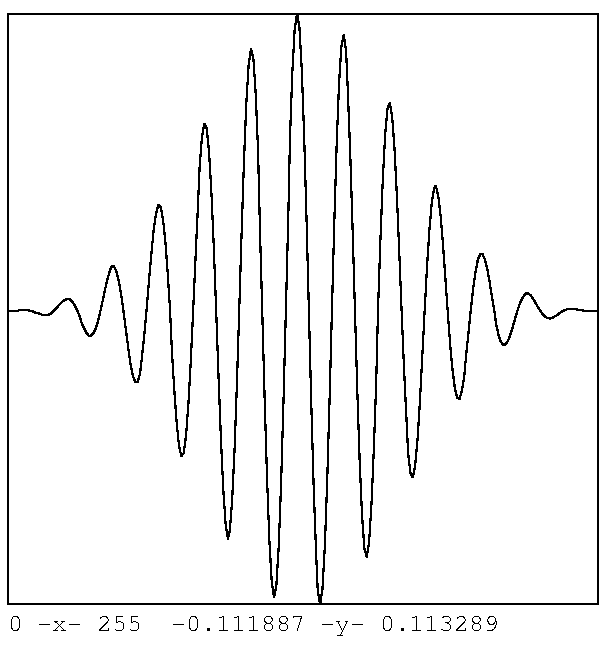
\includegraphics[width=6cm]{fig/window_1.pdf}
\end{center}
\par
This example passes the excitation generated through a train pulse
by a digital filter, applies a Blackman windowing function to it,
evaluates the log magnitude spectrum through 512 points FFT,
and plots the results on the screen:
\begin{quote}
\verb!train -p 50 | dfs -a 1 0.9 | window -l 50 -L 512 |\! \\
\verb!spec -l 512 | fdrw | xgr!
\end{quote}
\begin{center}
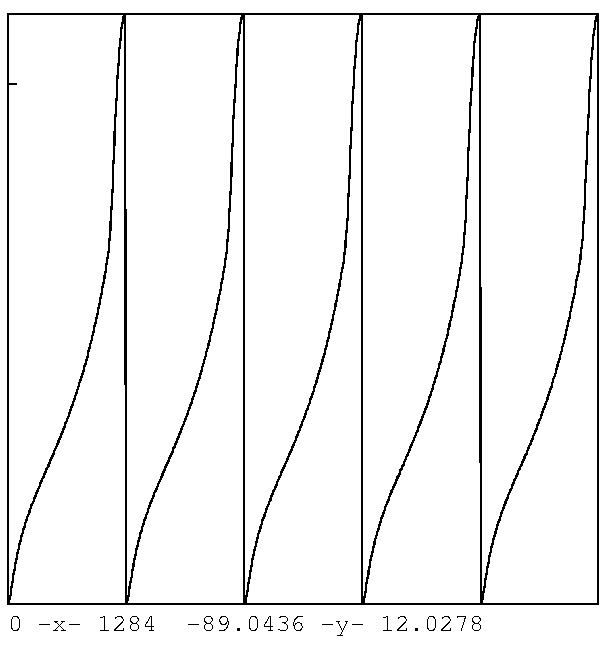
\includegraphics[width=6cm]{fig/window_2.pdf}
\end{center}
\end{qsection}

\begin{qsection}{SEE ALSO}
\hyperlink{fftr}{fftr},
\hyperlink{spec}{spec}
\end{qsection}

% ----------------------------------------------------------------- %
%             The Speech Signal Processing Toolkit (SPTK)           %
%             developed by SPTK Working Group                       %
%             http://sp-tk.sourceforge.net/                         %
% ----------------------------------------------------------------- %
%                                                                   %
%  Copyright (c) 1984-2007  Tokyo Institute of Technology           %
%                           Interdisciplinary Graduate School of    %
%                           Science and Engineering                 %
%                                                                   %
%                1996-2013  Nagoya Institute of Technology          %
%                           Department of Computer Science          %
%                                                                   %
% All rights reserved.                                              %
%                                                                   %
% Redistribution and use in source and binary forms, with or        %
% without modification, are permitted provided that the following   %
% conditions are met:                                               %
%                                                                   %
% - Redistributions of source code must retain the above copyright  %
%   notice, this list of conditions and the following disclaimer.   %
% - Redistributions in binary form must reproduce the above         %
%   copyright notice, this list of conditions and the following     %
%   disclaimer in the documentation and/or other materials provided %
%   with the distribution.                                          %
% - Neither the name of the SPTK working group nor the names of its %
%   contributors may be used to endorse or promote products derived %
%   from this software without specific prior written permission.   %
%                                                                   %
% THIS SOFTWARE IS PROVIDED BY THE COPYRIGHT HOLDERS AND            %
% CONTRIBUTORS "AS IS" AND ANY EXPRESS OR IMPLIED WARRANTIES,       %
% INCLUDING, BUT NOT LIMITED TO, THE IMPLIED WARRANTIES OF          %
% MERCHANTABILITY AND FITNESS FOR A PARTICULAR PURPOSE ARE          %
% DISCLAIMED. IN NO EVENT SHALL THE COPYRIGHT OWNER OR CONTRIBUTORS %
% BE LIABLE FOR ANY DIRECT, INDIRECT, INCIDENTAL, SPECIAL,          %
% EXEMPLARY, OR CONSEQUENTIAL DAMAGES (INCLUDING, BUT NOT LIMITED   %
% TO, PROCUREMENT OF SUBSTITUTE GOODS OR SERVICES; LOSS OF USE,     %
% DATA, OR PROFITS; OR BUSINESS INTERRUPTION) HOWEVER CAUSED AND ON %
% ANY THEORY OF LIABILITY, WHETHER IN CONTRACT, STRICT LIABILITY,   %
% OR TORT (INCLUDING NEGLIGENCE OR OTHERWISE) ARISING IN ANY WAY    %
% OUT OF THE USE OF THIS SOFTWARE, EVEN IF ADVISED OF THE           %
% POSSIBILITY OF SUCH DAMAGE.                                       %
% ----------------------------------------------------------------- %
\hypertarget{x2x}{}
\name{x2x}{data type transformation}{data operation}

\begin{synopsis}
\item[x2x] [ +$type1$ ] [ +$type2$ ] [ $\%format$ ] [ +a{\em $N$} ] [ --r ]
\end{synopsis}

\begin{qsection}{DESCRIPTION}
{\em x2x} converts data from standard input to a different data type,
sending the result to standard output.

The input and output data type are specified by command line options 
as described below.
\end{qsection}

\begin{options}
	\argp{type1}{input data type}{f}
	\argp{type2}{output data type\\
	both options $type1, type2$ can be assigned.
        one of the options below.\\
                \begin{tabular}{llcll} \\[-1ex]
                        c & char (1 byte) & \quad &
                        C & unsigned char (1 byte) \\
                        s & short (2 bytes) & \quad &
                        S & unsigned short (2 bytes) \\
                        i3 & int (3 bytes) & \quad &
                        I3 & unsigned int (3 bytes) \\		 
                        i & int (4 bytes) & \quad &
                        I & unsigned int (4 bytes) \\
                        l & long (4 bytes) & \quad &
                        L & unsigned long (4 bytes) \\
                        le & long long (8 bytes) & \quad &
                        LE & unsigned long long (8 bytes) \\
                        f & float (4 bytes) & \quad &
                        d & double (8 bytes) \\
                        de & long double (12 bytes) & \quad &
                        a & ASCII \\
                       aN & ASCII specifying the & \quad & & \\
                          & column number $N$  & & & \\ [1ex]
                \end{tabular} \\
                data type is converted from $t_1(type_1)$ to $t_2(type_2)$.
                if $t_2$ is not assigned then no operation is
                performed, and the output file is equal to the input
                file.}{type1}
	\argm{r}{}{specify rounding off when a real number
                 is substituted for an integer}{FALSE}
	\argm{o}{}{clip by minimum and maximum of output data type
                 if input data is over the range of output data
                 type. if the -o option is not given, when the data type lengths
 are different, the process will be aborted.}{FALSE}
 \argp{{\bf a}\%format}{specify output format similar to 'printf()', 
                           only if $type2$ is ASCII.}{$\%g$}
\end{options}

\begin{qsection}{EXAMPLE}
The following example converts data in ASCII format
read from {\em data.asc} into float format,
and writes the output to {\em data.f}:
\begin{quote}
  \verb!x2x +af < data.asc > data.f!
\end{quote}
\par
This example reads data in float format from {\em data.f},
converts it to ASCII format, and sends the output to the screen:
\begin{quote}
  \verb!x2x +fa < data.f!
\end{quote}
For example, if the contents of {\em data.f} in float format are
\begin{displaymath}
  1, 2, 3, 4, 5, 6, 7
\end{displaymath}
then the following output is printed to the screen.
\begin{quote}
  \verb!1! \\
  \verb!2! \\
  \verb!3! \\
  \verb!4! \\
  \verb!5! \\
  \verb!6! \\
  \verb!7!
\end{quote}
\par
If for the same data in the example above,
the number of columns is assigned:
\begin{quote}
  \verb!x2x +fa3 < data.f!
\end{quote}
the output will be:
\begin{quote}
  \verb!1       2        3! \\
  \verb!4       5        6! \\
  \verb!7!
\end{quote}
\par
The output uses the printf command \%e format:
\begin{quote}
  \verb!x2x +fa%9.4e < data.f!
\end{quote}
In this example the total number of characters for each number
is 11, and the number of decimal points assigned to 4.
\begin{quote}
  \verb!1.0000e+000! \\
  \verb!2.0000e+000! \\
  \mbox{\hspace{2em}}$\vdots$ \\
  \verb!7.0000e+000!
\end{quote}
\par
By using -r option, the result can be rounded off.
For example, suppose that the contents of {\em data.f} in float format are
\begin{displaymath}
  1.2,\; 2.3,\; 3.4,\; 4.5,\; 5.6,\; 6.7,\; 7.8.
\end{displaymath}
By the following command line without -r option,
\begin{quote}
  \verb!x2x +fs < data.f!
\end{quote}
the result will be
\begin{displaymath}
  1,\; 2,\; 3,\; 4,\; 5,\; 6,\; 7.
\end{displaymath}
This shows that the decimal points in {\em data.f} is suppressed.
On the other hand, without -r option,
\begin{quote}
  \verb!x2x +fs -r < data.f!
\end{quote}
the result will be
\begin{displaymath}
  1,\; 2,\; 3,\; 5,\; 6,\; 7,\; 8.
\end{displaymath}
This shows that each data in {\em data.f} are rounded off.
\par
In the following example, the result can be clipped by -o option.
\begin{quote}
  \verb! echo '126 127 128 -127 -128 -129' > data.ascii! \\
  \verb! x2x +ac -o < data.ascii!
\end{quote}
The result will be:
\begin{displaymath}
 126,\; 127,\; 127,\; -127,\; -128,\; -128,
\end{displaymath}
where 128 and -129 in {\em data.ascii} are clipped by the maximum and minimum of
char type, that is, 127 and -128, respectively.
\end{qsection}

\begin{qsection}{SEE ALSO}
\hyperlink{dmp}{dmp}
\end{qsection}

% ----------------------------------------------------------------
%       Speech Signal Processing Toolkit (SPTK): version 3.0
%                      SPTK Working Group
% 
%                Department of Computer Science
%                Nagoya Institute of Technology
%                             and
%   Interdisciplinary Graduate School of Science and Engineering
%                Tokyo Institute of Technology
%                   Copyright (c) 1984-2000
%                     All Rights Reserved.
% 
% Permission is hereby granted, free of charge, to use and
% distribute this software and its documentation without
% restriction, including without limitation the rights to use,
% copy, modify, merge, publish, distribute, sublicense, and/or
% sell copies of this work, and to permit persons to whom this
% work is furnished to do so, subject to the following conditions:
% 
%   1. The code must retain the above copyright notice, this list
%      of conditions and the following disclaimer.
% 
%   2. Any modifications must be clearly marked as such.
%                                                                        
% NAGOYA INSTITUTE OF TECHNOLOGY, TOKYO INSITITUTE OF TECHNOLOGY,
% SPTK WORKING GROUP, AND THE CONTRIBUTORS TO THIS WORK DISCLAIM
% ALL WARRANTIES WITH REGARD TO THIS SOFTWARE, INCLUDING ALL
% IMPLIED WARRANTIES OF MERCHANTABILITY AND FITNESS, IN NO EVENT
% SHALL NAGOYA INSTITUTE OF TECHNOLOGY, TOKYO INSITITUTE OF
% TECHNOLOGY, SPTK WORKING GROUP, NOR THE CONTRIBUTORS BE LIABLE
% FOR ANY SPECIAL, INDIRECT OR CONSEQUENTIAL DAMAGES OR ANY
% DAMAGES WHATSOEVER RESULTING FROM LOSS OF USE, DATA OR PROFITS,
% WHETHER IN AN ACTION OF CONTRACT, NEGLIGENCE OR OTHER TORTIOUS
% ACTION, ARISING OUT OF OR IN CONNECTION WITH THE USE OR
% PERFORMANCE OF THIS SOFTWARE.
% ----------------------------------------------------------------
%
\hypertarget{xgr}{}
\name{xgr}{XY-plotter simulator for X-window system}{plotting graphs}

\begin{synopsis}
 \item[xgr]   [ --s {\em S} ] [ --l ] [ --rv ] [ --m ] [ --bg {\em BG} ]
              [ --hl {\em HL} ] [ --bd {\em BD} ] 
 \item[\ ~~~~] [ --ms {\em MS} ] [ --g {\em G} ] [ --d {\em D} ]
              [ --t {\em T} ] [ {\em infile} ]
\end{synopsis} 

\begin{qsection}{DESCRIPTION}
{\em xgr} plots a graph from a sequence of FP5301 plotter commands, 
displaying the output on the screen in a new X window.

When the X window is created, 
the keyboard focus is initially assigned to that new window, 
which responds to a limited set of user interactions:
\begin{itemize}
\item Changing the window size truncates or expands the area 
	in which the graph is displayed, 
	but the graph stays the same size; 
	it is not rescaled to fit the new window size.
\item If the graph is larger than the window, 
	the position within the window can be changed with 
	``vi'' cursor movement commands:
\begin{quote}
		h: left scroll\\
		j: down scroll\\
		k: up scroll\\
		l: right scroll
\end{quote}
\item To delete the window, type one of the following:
	``q'',``Ctrl-c'',``Ctrl-d''
\end{itemize}
\end{qsection}

\begin{options}
	\argm{s}{S}{shrink}{3.38667}
	\argm{l}{}{landscape}{FALSE}
	\argm{rv}{}{reverse mode}{FALSE}
	\argm{m}{}{monochrome display mode}{FALSE}
	\argm{bg}{BG}{background color}{white}
	\argm{hl}{HL}{highlight color}{blue}
	\argm{bd}{BD}{border color}{blue}
	\argm{ms}{MS}{mouse color}{red}
	\argm{g}{G}{geometry}{NULL}
	\argm{d}{D}{display}{NULL}
	\argm{t}{T}{window title}{xgr}
\end{options}
\begin{qsection}{EXAMPLE}
The following example uses ``fdrw'' to draw a graph based on data read
from {\em data.f}, and sends the output in a X-Window environment:
\begin{quote}
 \verb!fdrw < data.f | xgr!
\end{quote}
\end{qsection}
\begin{qsection}{BUGS}
\begin{itemize}
\item If the display server does not contain backing store function,
then the hidden part of virtual screen is erased.

\item To lessen the waiting time to display graphs,
a image of virtual screen is copied to the memory.
If the size assigned by the --g option is too small
or if during the time the graph is being plotted an another window
is put above the virtual screen, then a part of virtual screen
will be erased.
The --s option is suggested whenever the size of
the virtual screen should be reduced.
\end{itemize}

\end{qsection}
\begin{qsection}{SEE ALSO}
\hyperlink{fig}{fig},
\hyperlink{fdrw}{fdrw}
\end{qsection}

% ----------------------------------------------------------------- %
%             The Speech Signal Processing Toolkit (SPTK)           %
%             developed by SPTK Working Group                       %
%             http://sp-tk.sourceforge.net/                         %
% ----------------------------------------------------------------- %
%                                                                   %
%  Copyright (c) 1984-2007  Tokyo Institute of Technology           %
%                           Interdisciplinary Graduate School of    %
%                           Science and Engineering                 %
%                                                                   %
%                1996-2008  Nagoya Institute of Technology          %
%                           Department of Computer Science          %
%                                                                   %
% All rights reserved.                                              %
%                                                                   %
% Redistribution and use in source and binary forms, with or        %
% without modification, are permitted provided that the following   %
% conditions are met:                                               %
%                                                                   %
% - Redistributions of source code must retain the above copyright  %
%   notice, this list of conditions and the following disclaimer.   %
% - Redistributions in binary form must reproduce the above         %
%   copyright notice, this list of conditions and the following     %
%   disclaimer in the documentation and/or other materials provided %
%   with the distribution.                                          %
% - Neither the name of the SPTK working group nor the names of its %
%   contributors may be used to endorse or promote products derived %
%   from this software without specific prior written permission.   %
%                                                                   %
% THIS SOFTWARE IS PROVIDED BY THE COPYRIGHT HOLDERS AND            %
% CONTRIBUTORS "AS IS" AND ANY EXPRESS OR IMPLIED WARRANTIES,       %
% INCLUDING, BUT NOT LIMITED TO, THE IMPLIED WARRANTIES OF          %
% MERCHANTABILITY AND FITNESS FOR A PARTICULAR PURPOSE ARE          %
% DISCLAIMED. IN NO EVENT SHALL THE COPYRIGHT OWNER OR CONTRIBUTORS %
% BE LIABLE FOR ANY DIRECT, INDIRECT, INCIDENTAL, SPECIAL,          %
% EXEMPLARY, OR CONSEQUENTIAL DAMAGES (INCLUDING, BUT NOT LIMITED   %
% TO, PROCUREMENT OF SUBSTITUTE GOODS OR SERVICES; LOSS OF USE,     %
% DATA, OR PROFITS; OR BUSINESS INTERRUPTION) HOWEVER CAUSED AND ON %
% ANY THEORY OF LIABILITY, WHETHER IN CONTRACT, STRICT LIABILITY,   %
% OR TORT (INCLUDING NEGLIGENCE OR OTHERWISE) ARISING IN ANY WAY    %
% OUT OF THE USE OF THIS SOFTWARE, EVEN IF ADVISED OF THE           %
% POSSIBILITY OF SUCH DAMAGE.                                       %
% ----------------------------------------------------------------- %
\hypertarget{zcross}{}
\name{zcross}{zero cross}{signal processing}

\begin{synopsis}
\item[zcross] [ --l $L$ ] [ --n ] [ {\em infile} ]
\end{synopsis}

\begin{qsection}{DESCRIPTION}
{\em zcross} determines the number of zero crossings 
within each length $L$ input vector, 
sending the result to standard output 
as one float number for each input vector.

Input and output data are in float format.
\end{qsection}

\begin{options}
	\argm{l}{L}{frame length\\
                    if $L \le 0$ then no data output.}{256}
	\argm{n}{}{normalized by frame length}{FALSE}
\end{options}

\begin{qsection}{EXAMPLE}
Data in float format is read from {\em data.f},
a zero crossing rate is computed,
and the results is written to {\em data.zc}:
\begin{quote}
  \verb!zcross < data.f > data.zc!
\end{quote}
\end{qsection}

\begin{qsection}{SEE ALSO}
\hyperlink{frame}{frame},
\hyperlink{spec}{spec}
\end{qsection}

% ----------------------------------------------------------------- %
%             The Speech Signal Processing Toolkit (SPTK)           %
%             developed by SPTK Working Group                       %
%             http://sp-tk.sourceforge.net/                         %
% ----------------------------------------------------------------- %
%                                                                   %
%  Copyright (c) 1984-2007  Tokyo Institute of Technology           %
%                           Interdisciplinary Graduate School of    %
%                           Science and Engineering                 %
%                                                                   %
%                1996-2015  Nagoya Institute of Technology          %
%                           Department of Computer Science          %
%                                                                   %
% All rights reserved.                                              %
%                                                                   %
% Redistribution and use in source and binary forms, with or        %
% without modification, are permitted provided that the following   %
% conditions are met:                                               %
%                                                                   %
% - Redistributions of source code must retain the above copyright  %
%   notice, this list of conditions and the following disclaimer.   %
% - Redistributions in binary form must reproduce the above         %
%   copyright notice, this list of conditions and the following     %
%   disclaimer in the documentation and/or other materials provided %
%   with the distribution.                                          %
% - Neither the name of the SPTK working group nor the names of its %
%   contributors may be used to endorse or promote products derived %
%   from this software without specific prior written permission.   %
%                                                                   %
% THIS SOFTWARE IS PROVIDED BY THE COPYRIGHT HOLDERS AND            %
% CONTRIBUTORS "AS IS" AND ANY EXPRESS OR IMPLIED WARRANTIES,       %
% INCLUDING, BUT NOT LIMITED TO, THE IMPLIED WARRANTIES OF          %
% MERCHANTABILITY AND FITNESS FOR A PARTICULAR PURPOSE ARE          %
% DISCLAIMED. IN NO EVENT SHALL THE COPYRIGHT OWNER OR CONTRIBUTORS %
% BE LIABLE FOR ANY DIRECT, INDIRECT, INCIDENTAL, SPECIAL,          %
% EXEMPLARY, OR CONSEQUENTIAL DAMAGES (INCLUDING, BUT NOT LIMITED   %
% TO, PROCUREMENT OF SUBSTITUTE GOODS OR SERVICES; LOSS OF USE,     %
% DATA, OR PROFITS; OR BUSINESS INTERRUPTION) HOWEVER CAUSED AND ON %
% ANY THEORY OF LIABILITY, WHETHER IN CONTRACT, STRICT LIABILITY,   %
% OR TORT (INCLUDING NEGLIGENCE OR OTHERWISE) ARISING IN ANY WAY    %
% OUT OF THE USE OF THIS SOFTWARE, EVEN IF ADVISED OF THE           %
% POSSIBILITY OF SUCH DAMAGE.                                       %
% ----------------------------------------------------------------- %
\hypertarget{zerodf}{}
\name{zerodf}{all zero digital filter for speech synthesis}{filters for
speech synthesis}

\begin{synopsis}
\item[zerodf] [ --m $M$ ] [ --p $P$ ] [ --i $I$ ] [ --t ] [ --k ]
		{\em bfile} [ {\em infile} ]
\end{synopsis}

\begin{qsection}{DESCRIPTION}
{\em zerodf} derives a standard-form FIR (all-zero) digital filter 
from the coefficients \\ $b(0), b(1), \dots, b(M)$ in {\em bfile} 
and uses it to filter an excitation sequence 
from {\em infile} (or standard input) to synthesize speech data, 
sending the result to standard output.

Input and output data are in float format.

The transfer function $H(z)$ of an FIR filter in standard form is
\begin{displaymath}
H(z) = \sum_{m=0}^{M} b(m) z^{-m}
\end{displaymath}
\end{qsection}

\begin{options}
	\argm{m}{M}{order of coefficients}{25}
	\argm{p}{P}{frame period}{100}
	\argm{i}{I}{interpolation period}{1}
	\argm{t}{}{transpose filter}{FALSE}
	\argm{k}{}{filtering without gain}{FALSE}
\end{options}

\begin{qsection}{EXAMPLE}
In the following example,
Excitation is generated from pitch information read in float format
from {\em data.pitch}. It is then passed through a FIR filter with
coefficients read from {\em data.b},
and the synthesized speech is written to {\em data.syn}:
\begin{quote}
  \verb!excite < data.pitch  | zerodf data.b > data.syn!
\end{quote}
\end{qsection}

\begin{qsection}{SEE ALSO}
\hyperlink{poledf}{poledf},
\hyperlink{lmadf}{lmadf}
\end{qsection}

%END COMMANDS

\cleardoublepage
\pagestyle{headings}
\begin{thebibliography}{99}

% $B2~NI%1%W%9%H%i%`K!(B

\bibitem{ref:icep-IECE}
$B:#0f(B $B@;(B, $B0$It(B $BK'=U(B,
``$B2~NI%1%W%9%H%i%`K!$K$h$k%9%Z%/%H%kJqMm$NCj=P(B,''
  $B?.3XO@(B(A), Vol.J62-A, No.4, pp.217--223, Apr. 1979.

% $BITJP?dDjK!(B

\bibitem{ref:UELS-IEICE}
$B:#0f(B $B@;(B, $B8E;T(B $B@i;^;R(B,
``$BBP?t%9%Z%/%H%k$NITJP?dDj(B,''
  $B?.3XO@(B(A), Vol.J70-A, No.3, pp.471--480, Mar. 1987.

\bibitem{ref:UELS-SignalProcessingIV}
S. Imai and C. Furuichi,
``Unbiased estimator of log spectrum
  and its application to speech signal processing,''
  Signal Processing IV: Theory and Applications,
  Vol.1, pp.203--206, Elsevire, North-Holland, 1988.

\bibitem{ref:acep-IEICE}
$BFAED(B $B7C0l(B, $B>.NS(B $BN4IW(B, $B1vK\(B $B>M;J(B, $B:#0f(B $B@;(B,
``$BE,1~%1%W%9%H%i%`J,@O(B --- $B%1%W%9%H%i%`$r78?t$H$9$kE,1~%U%#%k%?(B ---,''
  $B?.3XO@(B(A), Vol.J73-A, No.7, pp.1207--1215, July 1990.

\bibitem{ref:acep-IEEESP}
K. Tokuda, T. Kobayashi and S. Imai,
``Adaptive cepstral analysis of speech,''
  IEEE Trans. Speech and Audio Process., Vol.3, No.6, pp.481--488, Nov. 1995.

% $B0lHL2=%1%W%9%H%i%`J,@O(B

\bibitem{ref:gcep-IEICE}
$BFAED(B $B7C0l(B, $B>.NS(B $BN4IW(B, $B;3K\(B $BN5B@O:(B, $B:#0f(B $B@;(B,
``$B0lHL2=%1%W%9%H%i%`$r%Q%i%a!<%?$H$9$k2;@<$N%9%Z%/%H%k?dDj(B,''
  $B?.3XO@(B(A), Vol.J72-A, No.3, pp.457--465, Mar. 1989.

\bibitem{ref:gcep-IEEEASSP}
T. Kobayashi and S. Imai,
``Spectral analysis using generalized cepstrum,''
  IEEE Trans. Acoust., Speech, Signal Process.,
  Vol.ASSP-32, No.5, pp.1087--1089, Oct. 1984.

\bibitem{ref:gcep-ICASSP90}
K. Tokuda, T. Kobayashi and S. Imai,
``Generalized cepstral analysis of speech
  --- A unified approach to LPC and cepstral method,''
  Proc. ICASSP-90, % Kobe, Japan,
  pp.37--40, 
  Nov. 1990.

\bibitem{ref:agcep-IEICEtaikai90s}
$B?<ED(B $B=SL@(B, $BFAED(B $B7C0l(B, $B>.NS(B $BN4IW(B, $B:#0f(B $B@;(B,
``$BE,1~0lHL2=%1%W%9%H%i%`J,@O$N8!F$(B,''
  1990$B?.3X=U5(A4Bg(B, pp.1-150, Mar. 1980.

% $B%a%k%1%W%9%H%i%`J,@O(B

\bibitem{ref:mcep-IEICE}
$BFAED(B $B7C0l(B, $B>.NS(B $BN4IW(B, $B?<ED(B $B=SL@(B, $B:XF#(B $BGnFA(B, $B:#0f(B $B@;(B,
``$B%a%k%1%W%9%H%i%`$r%Q%i%a!<%?$H$9$k2;@<$N%9%Z%/%H%k?dDj(B,'' 
  $B?.3XO@(B(A), Vol.J74-A, No.8, pp.1240--1248, Aug. 1991.

\bibitem{ref:amcep-IEICE}
$BFAED(B $B7C0l(B, $B>.NS(B $BN4IW(B, $B?<ED(B $B=SL@(B, $B:#0f(B $B@;(B,
``$B2;@<$NE,1~%a%k%1%W%9%H%i%`J,@O(B,''
  $B?.3XO@(B(A), Vol.J74-A, No.8, pp.1249--1256, Aug. 1991.

\bibitem{ref:amcep-ICASSP92}
T. Fukada, K. Tokuda, T. Kobayashi and S. Imai, 
``An Adaptive Algorithm for Mel-Cepstral Analysis of Speech,''
  Proc. ICASSP-92, % San Francisco, USA, 
  pp.137--140, %
  Mar. 1992.

% $B%a%k0lHL2=%1%W%9%H%i%`J,@O(B

\bibitem{ref:mgcep-IEICE}
$BFAED(B $B7C0l(B, $B>.NS(B $BN4IW(B, $B@iMU(B $B7z;J(B, $B:#0f(B $B@;(B,
``$B%a%k0lHL2=%1%W%9%H%i%`J,@O$K$h$k2;@<$N%9%Z%/%H%k?dDj(B,'' 
  $B?.3XO@(B(A), Vol.J75-A, No.7, pp.1124--1134, July 1992.

\bibitem{ref:mgcep-ICSLP94}
K. Tokuda, T. Kobayashi, T. Masuko and S. Imai,
``Mel-generalized cepstral analysis
  --- A unified approach to speech spectral estimation,''
  Proc. ICSLP-94, pp.1043--1046, Sep. 1994.

% 2$B<!%*!<%k%Q%94X?t$rMQ$$$?%a%k%1%W%9%H%i%`J,@O(B

\bibitem{ref:smcep-IEICE}
$B<c;R(B $BIp;N(B, $BFAED(B $B7C0l(B, $B1W;R(B $B5.;K(B, $B>.NS(B $BN4IW(B, $BKLB<(B $B@5(B,
``$BBP?t%9%Z%/%H%k$NG$0U4pDl4X?t$K$h$kE83+$K4p$E$/2;@<$N%9%Z%/%H%k?dDj(B,''
  $B?.3XO@(B(A), Vol.J82-D-II, No.12, pp.2203--2211, Dec. 1999.


% LMA$B!$(BMLSA$B!$(BMGLSA $B%U%#%k%?(B

\bibitem{ref:LMA-IECE}
$B:#0f(B $B@;(B,
``$BBP?t?6I}6a;w(B(LMA)$B%U%#%k%?(B,''
  $B?.3XO@(B(A), vol.J63-A, no.12, pp.886--893, Dec. 1980.

\bibitem{ref:MLSA-IECE}
$B:#0f(B $B@;(B, $B=;ED(B $B0lCK(B, $B8E;T(B $B@i;^;R(B,
``$B2;@<9g@.$N$?$a$N%a%kBP?t%9%Z%/%H%k6a;w(B(MLSA)$B%U%#%k%?(B,''
  $B?.3XO@(B(A), vol.J66-A, no.2, pp.122--129, Feb. 1983.

\bibitem{ref:MGLSA-IECE}
$B>.NS(B $BN4IW(B, $B:#0f(B $B@;(B, $BJ!ED(B $BK-(B, 
``$B%a%k0lHL2=BP?t%9%Z%/%H%k6a;w(B(MGLSA)$B%U%#%k%?(B,''
  $B?.3XO@(B(A), Vol.J68-A, No.6, pp.610--611, June 1985.

% $B%Q%i%a!<%?@8@.(B

\bibitem{ref:synHMM-ASJ}
$BFAED(B $B7C0l(B, $B1W;R(B $B5.;K(B, $B>.NS(B $BN4IW(B, $B:#0f(B $B@;(B, 
``$BF0E*FCD'$rMQ$$$?(B HMM $B$+$i$N2;@<%Q%i%a!<%?@8@.%"%k%4%j%:%`(B,''
  $BF|K\2;6A3X2q;o(B, vol.53, no.3, pp.192--200, Mar. 1997.

\bibitem{ref:synHMM-EUROSPEECH95}
K. Tokuda, T. Masuko, T. Yamada, T. Kobayashi and S. Imai,
``An algorithm for speech parameter generation
  from continuous mixture HMMs with dynamic features,''
  Proc. EUROSPEECH-95, pp.757--760, Sep. 1995.

\end{thebibliography}


\appendix
\chapter*{Block diagram of SPTK commands}%

Mitch Bradley kindly provided us the follwoing diagram to help users understand
and remember the relationships between the SPTK commands and data representations.

\vspace{1.0cm} 

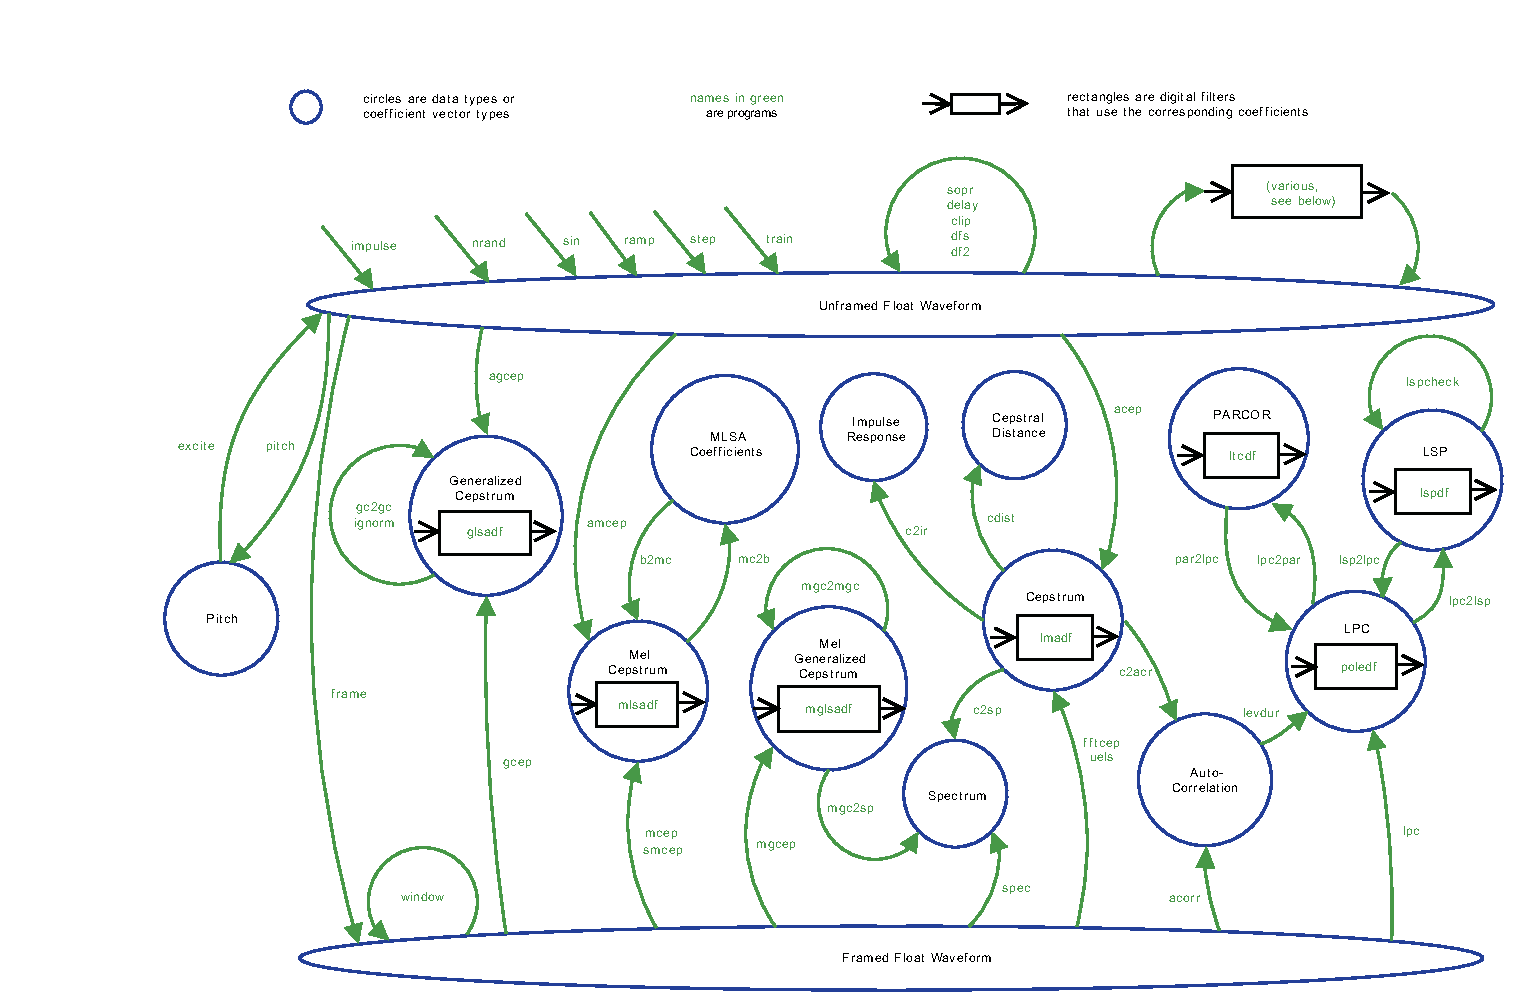
\includegraphics[width=16.5cm]{fig/sptk_sigproc.eps} 


\backmatter

\cleardoublepage
\printindex

\end{document}
